%%%%%%%%% espcrc1.tex %%%%%%%%%%
%
% $Id: espcrc1.tex 1.2 2000/07/24 09:12:51 spepping Exp spepping $
%
\documentclass[a4paper,12pt]{report}
\usepackage{footnote}
\usepackage{graphics}
\usepackage{sidecap}
\usepackage{layouts}
\usepackage{epsf}
\usepackage{epsfig}
\input epsf
\usepackage{times}
\usepackage[T1]{fontenc}
\usepackage[latin1]{inputenc}
\usepackage{geometry}
%\geometry{verbose,tmargin=0.7in,bmargin=0.5in,lmargin=0.4in,rmargin=0.4in}
%\setcounter{secnumdepth}{3}
%\setcounter{tocdepth}{3}
\geometry{verbose,a4paper,tmargin=1in,bmargin=1in,lmargin=1.in,rmargin=0.7in}
\usepackage{graphicx,psfrag}
\usepackage{setspace}
\usepackage{epsf}
\usepackage{amsmath}
\usepackage{amssymb}
\usepackage{bm}
%\doublespacing
\usepackage{rotating}
\raggedbottom
\textwidth  6.0 in
\textheight 8.5 in
%\oddsidemargin 0.15in
%\makeatletter
\newcommand{\plus}{\raisebox{.3\height}{\scalebox{.6}{+}}}
\newcommand{\minus}{\raisebox{0\height}{\scalebox{1}{-}}}
\begin{document}
%\pagestyle{empty}
\begin{flushright}
\vspace{-1cm}
\centerline{New Research Proposal to Jefferson Lab PAC 44}
\def\beqn{\begin{eqnarray}}
\def\eeqn{\end{eqnarray}}

\def\Journal#1#2#3#4{{#1} {\bf #2} (#4) #3 }
\def\PPNP{{ Prog. Part. Nucl. Phys.}}
\def\NIMA{{ Nucl. Instrum. Meth.} A}
\def\NIMB{{ Nucl. Instrum. Meth.} B}
\def\NCA{{ Nuovo Cimento} A}
\def\PHYS{{ Physica}}
\def\NPA{{ Nucl. Phys.} A}
\def\MATH{{ J. Math. Phys.}}
\def\PRO{{ Prog. Theor. Phys.}}
\def\NPB{{ Nucl. Phys.} B}
\def\PLA{{ Phys. Lett.} A}
\def\PLB{{ Phys. Lett.} B}
\def\PLD{{ Phys. Lett.} D}
\def\PL{{ Phys. Lett.}}
\def\PRL{ Phys. Rev. Lett.}
\def\PREV{ Phys. Rev.}
\def\PREP{ Phys. Rep.}
\def\PRA{{ Phys. Rev.} A}
\def\PRD{{ Phys. Rev.} D}
\def\PRC{{ Phys. Rev.} C}
\def\PRB{{ Phys. Rev.} B}
\def\ZPC{{ Z. Phys.} C}
\def\ZPA{{ Z. Phys.} A}
\def\ANNP{ Ann. Phys. (N.Y.)}
\def\RMP{{ Rev. Mod. Phys.}}
\def\CHEM{{ J. Chem. Phys.}}
\def\INT{{ Int. J. Mod. Phys.} E}
\def\INTA{{ Int. J. Mod. Phys.} A}
\def\EPJC{{ Eur. Phys. J.} C}
\def\JHEP{{ JHEP}}
\def\SJNP{{ Sov. J. Nucl. Phys.}}
%
\newcommand{\la}{\langle}
\newcommand{\ra}{\rangle}
\newcommand{\zh}{z}
\newcommand{\xbj}{x_{\scriptscriptstyle B}}
%
\newcommand{\Epgb}{$\vec ep~\rightarrow~ep(p,\Delta, N^*)\gamma~$}
\newcommand{\Epgl}{$\vec e\vec p~\rightarrow~ep(p,\Delta, N^*)\gamma~$}
\newcommand{\Eppiz}{$ep~\rightarrow~ep\pi^0~$}
\newcommand{\Enpip}{$ep~\rightarrow~en\pi^+~$}
\newcommand{\EppiD}{$ep~\rightarrow~e\pi \Delta~$}
\newcommand{\Epeta}{$ep~\rightarrow~ep\eta~$}
\newcommand{\Epr}{$ep~\rightarrow~ep\rho~$}
\newcommand{\EpX}{$ep\rightarrow epX~$}
\newcommand{\EpKY}{$ep~\rightarrow~eKY~$}
\newcommand{\vEpg}{$\vec ep~\rightarrow~ep\gamma~$}
\newcommand{\xidef}{$\xi=x_B\frac{1+\frac{Delta^2}{2Q^2}}{2-x_B+x_B\frac{Delta^2}{2Q^2}}$}
\def\gevc2{(GeV/c)$^2$}
\newcommand{\EpgX}{$ep~\rightarrow~ep\gamma X~$}
%%%%%%%%%%%%%%%%%%%%%%%%%%%%%%%%%%%%%%%%%%%%%%%%%%%

\renewcommand{\topfraction}{0.95}
\renewcommand{\bottomfraction}{0.95}
\renewcommand{\textfraction}{0.05}
\renewcommand{\floatpagefraction}{0.95}
\end{flushright}

\bigskip
%\vskip 0.5cm
{\Large{\centerline {\bf Proposal of extension of the CLAS12 run-group Cb (ND$_3$ target)}}}
%{\Large{\centerline {\bf CLAS12 and a longitudinally polarized deuterium target}}}

\vskip 0.5cm

\centerline{S. Niccolai\footnote{co-spokesperson}$^,$\footnote{contact person, email: silvia@jlab.org}, G. Charles, R. Dupr\'e, M. Guidal,}
\centerline{D. Marchand, C. Munoz Camacho, E. Voutier}
\centerline{\it Institut de Physique Nucl\'eaire d'Orsay, 91406 Orsay, France}
\vskip 0.4cm
\centerline{A. Biselli\footnotemark[1]}
\centerline{\it Fairfield University, Fairfield Connecticut 06824}
\vskip 0.4cm
\centerline{C. Keith\footnotemark[1], H. Avakian, V. Burkert, A. Deur, F.X. Girod, L. Elouadrhiri,} 
\centerline{V. Kubarovsky, K. Park, P. Rossi, S. Stepanyan, M. Ungaro}
\centerline{\it Thomas Jefferson National Laboratory, Newport News, VA 23606}
\vskip 0.4cm
\centerline{S. Pisano\footnotemark[1], V. Lucherini, M. Mirazita}
\centerline{\it INFN, Laboratori Nazionali di Frascati, 00044 Frascati, Italy}
\vskip 0.4cm
\centerline{D. Sokhan\footnotemark[1], D. Ireland, D. McGregor, B. McKinnon, G. Murdoch, B. Seitz}
\centerline{\it University of Glasgow, Glasgow, Scotland}
\vskip 0.4cm
\centerline{S. Kuhn\footnotemark[1]}
\centerline{\it Old Dominion University, Norfolk, VA 23529}
\vskip 0.4cm
\centerline{M. Battaglieri, A. Celentano, R. De Vita, E. Fanchini, M. Osipenko, M. Ripani, M. Taiuti}
\centerline{\it Istituto Nazionale di Fisica Nucleare, Sezione di Genova and }
\centerline{\it Dipartimento di Fisica, Universit\`a di Genova, Genova, Italy 16146}
\vskip 0.4cm
\centerline{D. Crabb, D. Day, D. Keller}
\centerline{\it University of Virginia, Charlottesville, VA 22904}
\vskip 0.4cm
\centerline{I. Balossino, L. Barion, G. Ciullo, M. Contalbrigo, P. Lenisa,}
\centerline{A. Movsysian, L. Pappalardo, M. Turisini}
\centerline{\it INFN, Istituto Nazionale di Fisica Nucleare, Sezione di Ferrara, Ferrara, Italy 44122}
\vskip 0.4cm
\centerline{A. D'Angelo, L. Lanza, A. Rizzo, I. Zonta}
\centerline{\it Universit\`a di Roma Tor Vergata and INFN Roma Tor Vergata, Roma, Italy 00133}
\vskip 0.4cm
\centerline{V. Bellini, F. Mammoliti, G. Russo, C.M. Sutera}
\centerline{\it Istituto Nazionale di Fisica Nucleare, Sezione di Catania, Catania, Italy 95123} 
\vskip 0.4cm
\centerline{J. Ball, M. Defurne, M. Gar\c{c}on, H. Moutarde, S. Procureur, F. Sabati\'e}
\centerline{\it CEA, Centre de Saclay, Irfu/Service de Physique Nucl\'eaire, 91191 Gif-sur-Yvette, France}
\vskip 0.4cm
\centerline{W.R. Armstrong, K. Hafidi, M. Hattawy}
\centerline{\it Argonne National Laboratory, Argonne, IL 60439}
\vskip 0.4cm
\centerline{P. Bosted, K. Griffioen}
\centerline{\it College of William and Mary, Williamsburg, VA 23187}
\vskip 0.4cm
\centerline{K. Slifer, E. Long, T. Badman, L. Hammed, M. Holtrop,}
\centerline{S. Li, D. Ruth, S. Santiesteban, R. Zielinski}
\centerline{\it University of New Hampshire, Durham, NH 03824}
\vskip 0.4cm
\centerline{T. Forest}
\centerline{\it Idaho State University, Pocatello, ID 83209}
\vskip 0.4cm
\centerline{K. Adhikari, L. El Fassi}
\centerline{\it Mississippi State University, Mississippi State, MS 39762 }
\vskip 0.4cm
\centerline{I. Skorodumina}
\centerline{\it University of South Carolina, Columbia, SC 29208}
\vskip 0.4cm
\centerline{G. Fetodov}
\centerline{\it Skobeltsyn Institute of Nuclear Physics, Lomonosov Moscow State, Russia}
\vskip 0.4cm
{\large{\centerline{\bf A CLAS Collaboration proposal}}}
\date{}

\abstract{The multi-dimensional mapping of the structure of the nucleon in terms of its partonic degrees of freedom is nowadays one of the main challenges of hadronic physics, and is at the core of the CLAS12 experimental program. Precise measurements of polarized parton distribution functions (PDFs) via deep inelastic scattering (DIS) give information on the spin content of the nucleon; the extraction of transverse momentum dependent distributions (TMDs) from semi-inclusive DIS (SIDIS) data provides the correlation between the transverse momentum and spin of the quarks; the generalized parton distributions (GPDs), accessible in exclusive electroproduction channels, finally, encode the interplay between the longitudinal momentum, the transverse position, and the spin of the quarks in the nucleon. An extensive experimental program geared towards the extraction of all the cited distributions is already scheduled for CLAS12, mainly on a proton target. In particular, 120 days on a polarized NH$_3$ target are approved. However, in order to perform the flavor separation of PDFs, TMDs, and GPDs, measurements on a neutron target, with comparable statistical precision, are necessary as well. This proposal aims at extending the running time of the approved run-group Cb, which currently provides 50 days of an 11-GeV electron beam impinging on a longitudinally polarized deuterium target (plus $\sim10$ days for target overhead and beam-polarization measurements), to 110 days of total duration (plus 23 days of overhead). For 50 days of the extension the same experimental setup of RG Cb will be used, with a beam current of 10 nA, while the Forward Tagger will be included for 10 days of low-luminosity running, at 5 nA. Assuming that run-group Cb includes a total of 60 days between production and ancillary runs, this proposal requests 73 new PAC days. The driving motivations for this extension are the measurements of single and double target-spin asymmetries for deeply virtual Compton scattering on longitudinally polarized neutrons (nDVCS), of double and single spin asymmetries for SIDIS (with both pions and kaons), and double spin asymmetries for DIS on the deuteron. Considering the lower polarization of the neutron on ND3 (40\%) with respect to the one of the proton in NH3 (80\%) and the smaller cross sections on neutrons than on protons, the overall neutron figure-of-merit is at least a factor of 4 smaller than for the proton. At a minimum, matching the integrated luminosity on protons with that on neutrons is necessary to perform the flavor separation of the aforementioned parton distributions, binned in the relevant kinematic variables. 
These data will also allow pioneering first-time measurements, such as polarized timelike Compton scattering, deeply-virtual meson electroproduction, and semi-inclusive di-hadron production off a longitudinally polarized neutron.}
\newpage
\tableofcontents{}
%\newpage
%\listoftables{} 
%\listoffigures{}
%\newpage
%\setcounter{page}{1}

\chapter{Run-group extension summary}
\section{Motivation for the run-group extension request}
This proposal is being submitted in response to the specific requests made by PAC43 in the report motivating the conditional approval of Experiment C12-15-004. 
Here we request the extension to 110 days, plus overhead, of the existing CLAS12 run-group Cb, which currently has 50 approved days of running of 11 GeV electron beam on a longitudinally polarized ND$_3$ target. 
The physics topics that will be studied thanks to this extensions cover two categories of the experimental program for the 12-GeV upgrade of Jefferson Lab: 
\begin{itemize}
\item{``The longitudinal structure of the hadrons (Unpolarized and polarized parton distribution functions - PDFs)'', with the measurement of deep inelastic scattering on longitudinally polarized deuterium (this proposal extends the already approved CLAS12 experiments E12-06-109 and E12-09-007b);}
\item{``The 3D structure of the hadrons (Generalized Parton Distributions - GPDs - and Transverse Momentum Distributions - TMDs)'', with the measurement of deeply virtual Compton scattering (DVCS) and semi-inclusive deep inelastic scattering (SIDIS) on longitudinally polarized neutron (for the SIDIS case, this proposal extends the already approved CLAS12 experiments E12-07-107 and E12-09-009).}
\end{itemize}
For both of these two categories, which are the main focus of the experimental program of CLAS12, the issue of quark-flavor separation of the three kinds of parton distributions extracted from the data (PDFs, GPDs, and TMDs) is fundamental. From the experimental point of view, flavor separation requires to take data to measure DIS, SIDIS and DVCS on both hydrogen and deuterium targets. Ideally, the statistical weight of proton and neutron data should be equal. The currently approved experimental program of CLAS12 foresees, on the one hand, an almost equal number of allocated days for unpolarized proton and deuterium targets (100 for the former, 80 for the latter). On the other hand, in the case of longitudinally polarized targets hydrogen has an allocated beam time (120 days) which is more than twice the one currently approved for deuterium (50 days). This discrepancy becomes even bigger considering that the polarization of the neutrons in ND$_3$ ($\sim 40$\%) is half of that of protons in NH$_3$ ($\sim 80$\%), and that the cross sections on the neutron are typically about half of those on the proton. Doubling the currently approved run-time on ND$_3$ will bring the deuteron statistics closer to that of the proton. 

In the case of DIS, increasing the statistics on polarized deuteron by a factor of two will reduce the uncertainty on polarized parton distributions for $d$ quarks, in the large-$x$ region, as well as for gluons and the strange quark sea at moderate-to-large $x$. This will be important to understand nuclear effects on the extraction of $\Delta d$ at high $x$, and to map out the asymptotic behavior of all quark distributions provided by Jefferson Lab's 12-GeV beam. 

In the case of SIDIS, the benefits of an increased statistics on ND$_3$ will be mostly evident in the high-$p_T$ region, where the existing TMD-based models are less constrained and their predictions for the SIDIS single and double target-spin asymmetries differ the most. Such benefits will be particularly important for the kaon channels, for which the statistics are considerably smaller than for pions. Moreover, the use of the Forward Tagger, for a subset of the running time, will impact very favorably the $\pi^0$ channel, increasing the coverage in the forward region. 

As far as DVCS is concerned, the neutron sector is basically unexplored, so far. An experiment to measure beam-spin asymmetries for neutron-DVCS with an unpolarized deuterium target is currently approved for CLAS12 (and labeled ``high impact'' by the PAC), but no measurements of single and double target-spin asymmetries exist nor are planned, as of today, for longitudinally polarized deuterium target. Combining DVCS observables measured at the same kinematic points allows to extract, in a model-independent way, the Compton Form Factors (CFFs), which are linked to the GPDs. 80 days are currently approved for unpolarized deuteron. In the polarized-target case, the maximum neutron luminosity achievable with CLAS12 is about an order of magnitude (3/20) smaller than for the unpolarized-target case, and the neutron polarization is $\sim 40$\%, but, on the plus side, the expected size of the target-spin asymmetry (TSA) for nDVCS is, on average, about a factor of 5 bigger than the beam-spin asymmetry (BSA): this means that matching the running time of unpolarized and polarized deuterium will lead to relative errors for the BSA and the TSA not too far off from each other (roughly a factor of 2 bigger relative errors for the TSA than for the BSA), and improve the coverage and precision on the extracted neutron CFFs. The utilization of the Forward Tagger in 10 of the 60 days of the extension, moreover, would permit to complete the $\phi$ coverage of the asymmetries, and thus the statistical precision on the extracted CFFs, especially for the low-$t$ kinematics, which are the most crucial for Ji's sum rule. The latter relates the total angular momentum of the quarks to the second moment in $x$ of the sum of two of the GPDs ($E$ and $H$), at $t=0$.

\section{Running conditions and beam-time request}
This extension request aims to reach a total of 110 days of production running on ND$_3$, plus 23 days of ``overhead'', which includes polarized-target maintenance, runs on carbon target for background studies, M\o ller runs to measure the beam polarization, and a few days of work to install the Forward Tagger. 

The beam current will be of 10 nA, corresponding to a total luminosity on ND$_3$ of $10^{35}$ cm$^{-2}$s$^{-1}$ and to a luminosity per neutron of $1.4 \cdot 10^{34}$ cm$^{-2}$s$^{-1}$, for 100 out of 110 days, and 5 nA for the remainder 10 days. 

The experimental setup for the already approved 50 days and for 50 more days that we request will remain unchanged (it includes the standard CLAS12 and the ND$_3$ longitudinally polarized target). For 10 of the 60 extra days of production running requested in this proposal, the inclusion of the Forward Tagger will allow to detect low-angle photons and thus increase the acceptance and precision at low $t$ for nDVCS observables, and also increase the coverage for the study of the $\pi^0$ channel in SIDIS. 

The beam-time request for the extended run-group Cb is detailed in Table~\ref{beam_time_summary}, in PAC days. 

\begin{table}
\begin{center}
\begin{tabular}{|c||c|}
%\hline
%Testing and commissioning & 2 days\\
\hline
Production data taking at $10^{35}$ cm$^{-2}$s$^{-1}$ on ND$_3$ & 100 days (50 of which are already approved)\\
\hline
Production data taking at $0.5\cdot 10^{35}$ cm$^{-2}$s$^{-1}$ on ND$_3$ & 10 days (with FT)\\
\hline
Target work & 8 days\\
\hline
Production data taking on $^{12}$C target & 10 days\\
\hline 
M\o ller polarimeter runs & 2 days\\
\hline
Configuration change & 3 days \\
\hline
\hline
Total beam time request & 133 days\\
\hline
\end{tabular}
\caption{Beam-time request for the extended of Run-group Cb, in PAC days, including the already approved 50 days on ND$_3$ and 23 days of overhead and calibration runs, which are shared between the approved RG and its extension.}
\label{beam_time_summary}
\end{center}
\end{table}

Assuming 60 PAC days in total, between production and ancillary runs, for the already approved part of run-group Cb \footnote{The number of days for production and ancillary runs varies for the various proposal constituing the presently approved run group Cb. 60 days is our own estimate, including 50 days of production running, 5 days of carbon data, 4 days of target work and 1 day of M\o ller runs.}, this extension proposal requests 73 PAC days of new beam time. 

\newpage
\chapter{Deeply Virtual Compton Scattering on the neutron with a longitudinally polarized deuteron target}
\centerline{Proposal presented following the conditional approval}
\centerline{of Experiment C12-15-004 by PAC 43}
\vskip 0.4cm
\centerline{S. Niccolai\footnote{contact person, email: silvia@jlab.org}}
\centerline{\it Institut de Physique Nucl\'eaire d'Orsay, 91406 Orsay, France}
%\vskip 0.4cm
%\centerline{A. Biselli\footnotemark[1]}
%\centerline{\it Fairfield University, Fairfield Connecticut 06824}
%\vskip 0.4cm
%\centerline{C. Keith\footnotemark[1]}
%\centerline{\it Thomas Jefferson National Laboratory, Newport News, VA 23606}
%\vskip 0.4cm
%\centerline{S. Pisano\footnotemark[1]}
%\centerline{\it INFN, Laboratori Nazionali di Frascati, 00044 Frascati, Italy}
%\vskip 0.4cm
%\centerline{D. Sokhan\footnotemark[1]}
%\centerline{\it University of Glasgow}
%\vskip 0.4cm

\abstract{Measurements of Deeply Virtual Compton Scattering on the neutron (nDVCS) are necessary for a complete description of nucleon structure in terms of Generalized Parton Distributions (GPDs). Combining DVCS results from both proton and neutron targets will permit the flavor decomposition of the GPDs. An experimental program of nDVCS has commenced at JLab with the already-approved experiment E12-11-003 to measure beam-spin asymmetries over a wide kinematic range using the CLAS12 detector. Here we propose to extend this program by measuring, for the first time, both target-spin and double-spin asymmetries for nDVCS using a longitudinally polarized deuteron target inside CLAS12. The measurements will be made detecting the electron and the photon in the forward part of CLAS12, which will be equipped also with the Forward Tagger during a subset of the experiment, and the recoil neutron in the recently completed Central Neutron Detector, thus assuring the exclusivity of the nDVCS reaction ($ed\to e'n\gamma(p)$). By fitting these results together with the beam-spin asymmetries measured by E12-11-003 at the same kinematic points, an extraction of several neutron Compton Form Factors (CFFs) can be made. $\Im{\rm m}({\cal E}_n)$ and $\Im{\rm m}({\cal H}_n)$ will be especially well determined thanks to their dominance in the beam- and target-spin asymmetries, respectively. Quark-flavor separation of the GPDs then becomes possible through a combination of the extracted neutron CFFs with those obtained from proton DVCS. In order to provide an accurate mapping of the nDVCS single and double target-spin asymmetries over the available 4-dimensional ($Q^2$ , $x_B$, $-t$, $\phi$) phase space, and thus achieve an accurate extraction of the neutron CFFs accessible from these observables, we request 60 more days of running on a ND$_3$ polarized target to add to the 50 existing ones of Run Group C of CLAS12, and to reach a total of 23 days of calibration, ancillary runs, and target overhead, with the maximum available beam energy of 11 GeV. This proposal was conditionally approved (C2) by PAC43, with the request to represent it at PAC44 split into a run-group proposal for the existing 50 days of Run-group Cb and an extension-request proposal for the additional days.}
\newpage
\setcounter{page}{8}  
\section{Introduction: Generalized Parton Distributions and DVCS}
Generalized Parton Distributions (GPDs) are nowadays the object of an intense 
effort of research, in the perspective of understanding nucleon structure.
The GPDs describe the correlations between the longitudinal momentum and transverse spatial position of the partons inside the nucleon, they give access to
the contribution of the orbital momentum of the quarks to the nucleon, and they are sensitive to the correlated $q-\bar{q}$ components.
The original articles and general reviews on GPDs and details of the formalism can be found in Refs.~\cite{muller}-\cite{revrady}.%~\cite{muller,ji,rady,collins,goeke,revdiehl,revrady}.

The nucleon GPDs are accessed in the measurement of the exclusive leptoproduction of a photon (DVCS, which stands for deeply virtual Compton scattering) or of a meson on the nucleon, at sufficiently large $Q^2$, where $Q^2$ is the virtuality of the photon emitted by the initial lepton, for the reaction to happen at the quark level. Figure~\ref{fig:dvcs} illustrates the leading process for DVCS, also called the ``handbag diagram''. At leading-order QCD and at leading twist, considering only quark-helicity conserving quantities and the quark sector, the process is described by four GPDs, $H^q, \tilde{H^q} , E^q, \tilde{E^q}$, one for each quark flavor $q$, that account for the possible combinations of relative orientations of nucleon spin and quark helicity between the initial and final state. $H$ and $E$ do not depend on the quark helicity and are therefore called unpolarized GPDs while $\tilde{H}$ and $\tilde{E}$ depend on the quark helicity and are called polarized GPDs. $H$ and $\tilde{H}$ conserve the spin of the nucleon, whereas $E$ and $\tilde{E}$ correspond to a nucleon-spin flip.

\begin{figure}[h]
\begin{center}
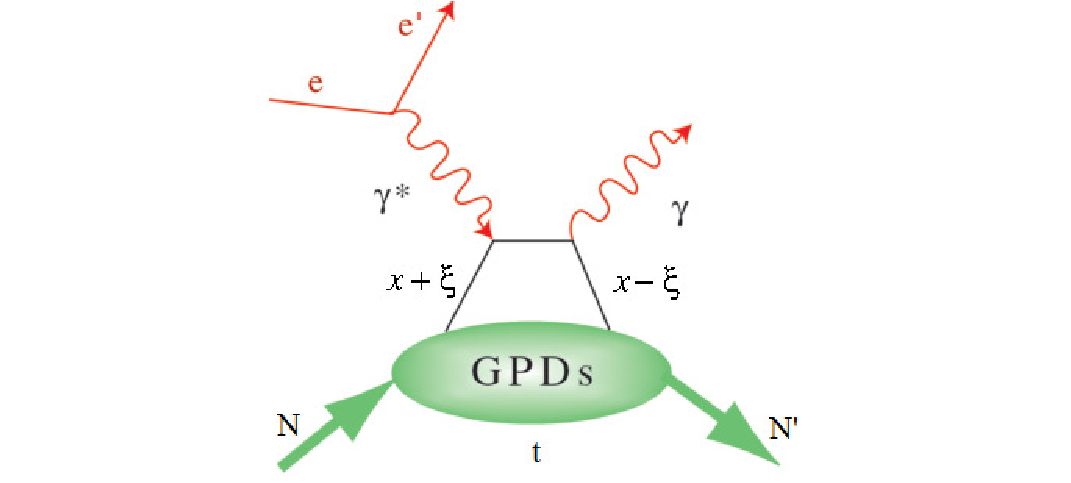
\includegraphics[scale=0.6]{handbag.pdf}
\caption[Handbag diagram for the DVCS process] {The handbag diagram for the DVCS process on the nucleon $eN\to e'N'\gamma'$. 
Here $x+\xi$ and $x-\xi$ are the longitudinal momentum fractions of the 
struck quark before and after scattering, respectively, and $t=(N-N')^2$ is the squared four-momentum transfer between the initial and final nucleons (or equivalently between the two photons).  In the Bjorken limit, i.e. for $Q^2=-q^2=-(k-k^\prime)^2\to \infty$ and $\nu = E_e-E_{e'} \to \infty$ so that the Bjorken scaling variable $x_B$ is finite, $\xi$ is proportional to $x_B$ ($\xi\simeq\frac{x_B}{2-x_B}$, where $x_B=\frac{Q^2}{2M\nu}$, $M$ is the nucleon mass and $\nu$ is the difference between the energies of the initial and final electron in the lab frame).}
\label{fig:dvcs}
\end{center}
\end{figure}

The GPDs depend upon three variables, $x$, $\xi$ and $t$: $x+\xi$ and $x-\xi$ are the longitudinal momentum fractions of the struck quark before and after scattering, respectively, and $t$ is the squared four-momentum transfer between the initial and final nucleon (see caption of Fig.~\ref{fig:dvcs} for the definitions of these variables). The transverse component of $t$ is the Fourier-conjugate variable of the transverse position of the struck parton in the nucleon. Among the three variables, $x$, $\xi$ and $t$, which appear in the DVCS formalism, only $\xi$ and $t$ are experimentally accessible in these reactions. 

The DVCS amplitude is proportional to combinations of integrals over $x$ of the form: 
\begin{equation}\label{dvcs-ampl}
\int_{-1}^{1} d x F(\mp x,\xi,t)\left[\frac{1}{x - \xi + i \epsilon}\pm\frac{1}{x + \xi - i \epsilon}\right]
\end{equation}
where $F$ represents one of the four GPDs. The top combination of the plus and minus signs applies to the quark-helicity independent, or unpolarized, GPDs ($H, E$), and the bottom combination of signs applies to the quark-helicity dependent, or polarized, GPDs ($\widetilde {H}, \widetilde {E}$). Each of these 4 integrals, which are called Compton Form Factors (CFFs), can be decomposed into their real and imaginary parts, as
\begin{eqnarray}\label{def_cffs1}
\Re{\rm e}{\cal F} (\xi,t)&=& {\cal P}\int_{-1}^{1}dx\left[\frac{1}{x-\xi}\mp\frac{1}{x+\xi}\right]F(x,\xi,t) \\
\Im{\rm m}{\cal F}(\xi,t)&=& -\pi [F(\xi,\xi,t)\mp F(-\xi,\xi,t)], \label{def_cffs2}
\end{eqnarray}

where ${\cal P}$ is Cauchy's principal value integral and the sign convention is the same as in Eq.~\ref{dvcs-ampl}. The information that can be extracted from the experimental data at a given ($\xi,t$) point depends on the observable involved. 
$\Re{\rm e}{\cal F}$ is accessed primarily measuring observables which are sensitive to the real part of the DVCS amplitude, such as double-spin asymmetries, beam-charge asymmetries or unpolarized cross sections. 
$\Im{\rm m}{\cal F}$ can be obtained measuring observables which are mainly sensitive to the imaginary part of the DVCS amplitude, such as single-spin asymmetries or cross-section differences. 

However, knowing the CFFs does not define the GPDs uniquely. A model input is necessary to deconvolute their $x$ dependence.

The DVCS process is accompanied by the Bethe-Heitler (BH) process, in which the final-state real photon is radiated by the incoming or scattered electron and not by the nucleon itself. The BH process, which is not sensitive to the GPDs, is experimentally indistinguishable from DVCS and interferes with it at the amplitude level. However, considering that the nucleon form factors are well known at small $t$, the BH process is precisely calculable.

\section{Physics motivation: neutron GPDs and flavor separation}
Measuring neutron GPDs is complementary to measuring proton GPDs, when using the DVCS reaction: %Measuring both sets of GPDs allows to carry out a quark-flavor separation. 
quark-flavor separation of the GPDs becomes possible only if both the proton and neutron GPDs are measured. 
Since we can express 
\begin{eqnarray}
{\cal H}^p(\xi, t)=\frac{4}{9}{\cal H}^u(\xi, t)+\frac{1}{9}{\cal H}^d(\xi, t)
\end{eqnarray}
and
\begin{eqnarray}
{\cal H}^n(\xi, t)=\frac{1}{9}{\cal H}^u(\xi, t)+\frac{4}{9}{\cal H}^d(\xi, t)  
\end{eqnarray}
(and similarly for ${\cal E}$, ${\tilde {\cal H}}$ and ${\tilde {\cal E}}$), it immediately follows that
\begin{eqnarray}
{\cal H}^u(\xi, t)=\frac{9}{15}(4 {\cal H}^p(\xi, t)-{\cal H}^n(\xi, t))
\end{eqnarray}
and
\begin{eqnarray}
{\cal H}^d(\xi, t)=\frac{9}{15}(4 {\cal H}^n(\xi, t)-{\cal H}^p(\xi, t)).  
\end{eqnarray}
An extensive experimental program devoted to the measurement of GPDs using the DVCS channel on a proton target has been approved at Jefferson Lab, in particular with CLAS12. Single-spin asymmetries with polarized beam and/or linearly or transversely polarized proton targets, as well as unpolarized and polarized cross sections, will be measured with high precision and a vast kinematic coverage. If a similar program is performed on the neutron, the flavor separation of the various GPDs will be possible. 
An experiment to measure the beam-spin asymmetry for nDVCS, particularly sensitive to the GPD $E_n$, has already been approved \cite{proposal}. The present proposal focuses on the extraction of two more observables, the target single-spin asymmetry and the (beam-target) double-spin asymmetry for nDVCS on a longitudinally polarized deuterium target. The next sections will outline those GPDs to which the nDVCS observables we plan to measure show the most sensitivity. 

\section{DVCS spin observables}\label{sec_dvcs_obs}
%\chead[\ref{sec_dvcs_obs} DVCS spin observables]{\let\uppercase\relax\leftmark}
A complete analysis of DVCS observables, including the asymmetries of interest in this document, in terms of Fourier harmonics with respect to the azimuthal angle, was carried out by Belitsky {\it et al.} \cite{belitski}, up to twist-3 approximation. 
These asymmetries allow the extraction of separate components of the azimuthal angular dependence of the $eN \to eN'\gamma$ cross section, which are related to the Compton Form Factors (CFFs) defined in Eqs.~\ref{def_cffs1}-\ref{def_cffs2}.% The cross section for exclusive photon production 
%\begin{eqnarray}
%\label{WQ}
%\frac{d\sigma}{d x_B dy dt d\phi}
%=
%\frac{\alpha^3  x_B y } {16 \, \pi^2 \,  Q^2 \sqrt{1 + \epsilon^2}}
%\left| \frac{\cal T}{e^3} \right|^2 \, 
%\end{eqnarray}
%depends on the Bjorken variable $x_B$, the squared momentum transfer $t =  (P_1 - P_2)^2$ (where $P_1$ and $P_2$ are the four-momenta of, respectively, the initial and final nucleon), the lepton energy fraction $y= P_1\cdot q_1/P_1\cdot k$, with $q_1 = k - k'$ (where $k$ and $k'$ are the four momenta of, respectively, the incoming and scattered electon) and the angle $\phi$, which is the angle between the leptonic and hadronic planes, as shown in Fig.~\ref{fig:dvcs_phi}. We define $\epsilon=2 x_B \frac{M}{Q}$. 
\begin{figure}[h]
\begin{center}
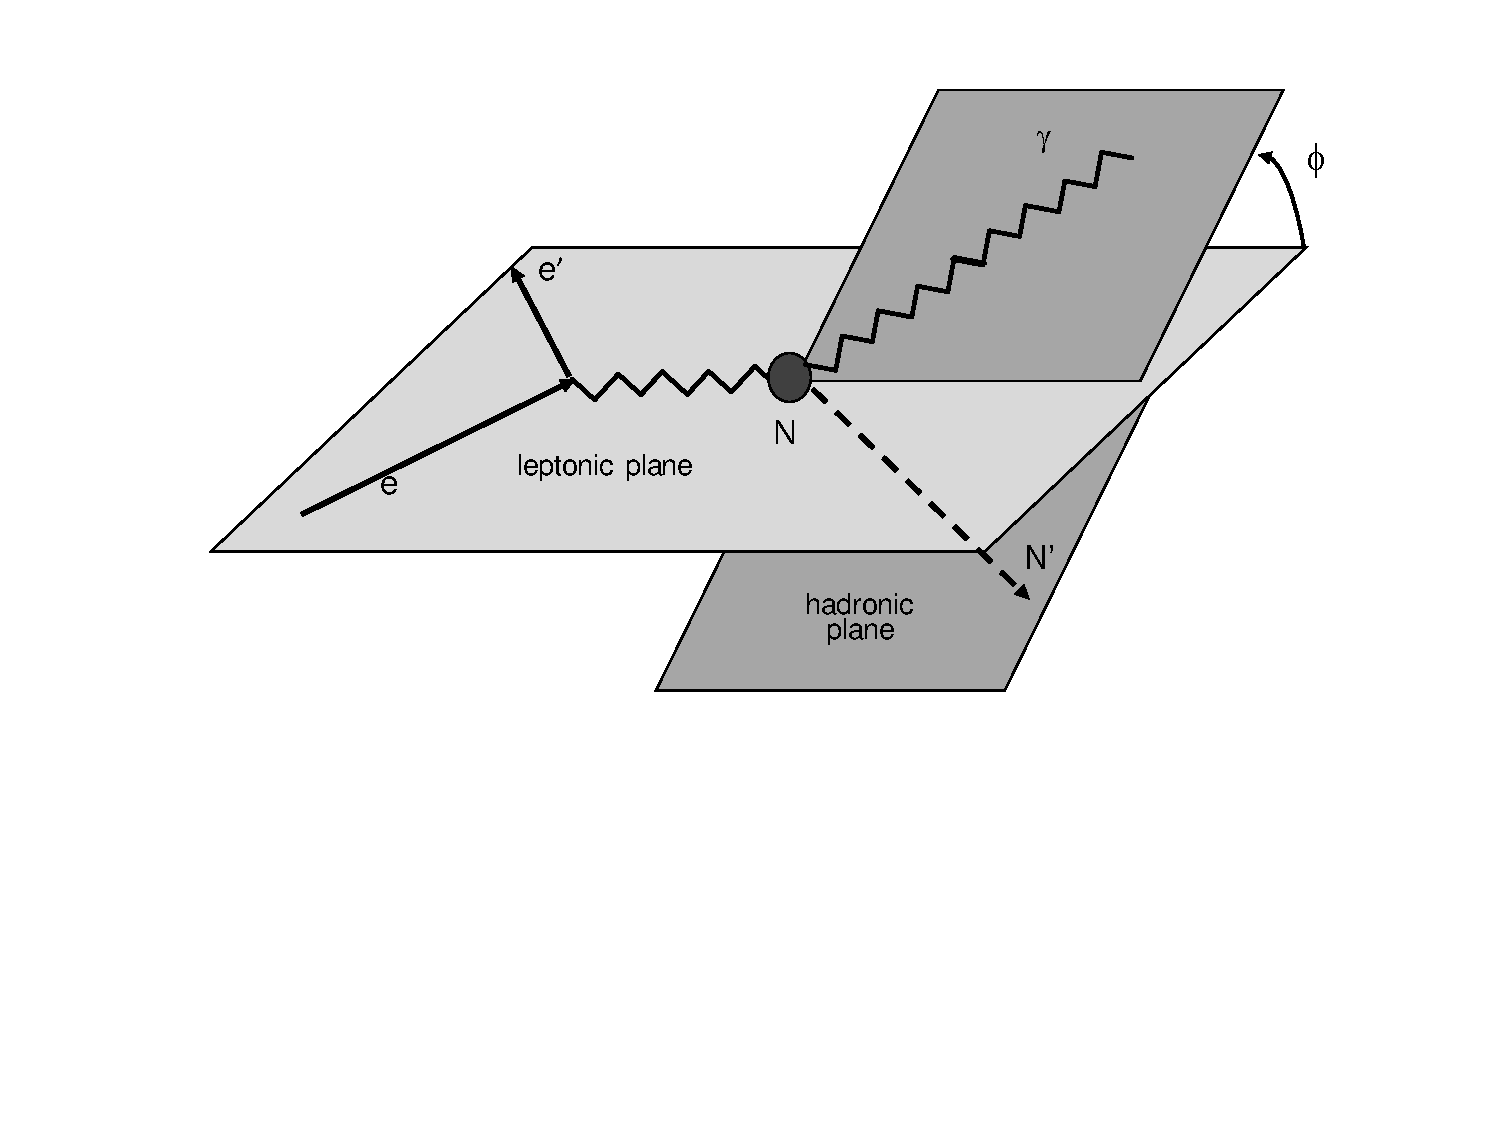
\includegraphics[width=120mm]{dvcs_diagram.pdf}
\vspace{-3.cm}
%\vskip -1cm
\caption[$eN \to eN'\gamma$ reaction plane.]{Schematic to illustrate the definition of the angle $\phi$, formed by the leptonic and hadronic planes, in the $eN \to eN'\gamma$ reaction.}
\label{fig:dvcs_phi}
\end{center}
\end{figure}

The amplitude ${\cal T}$ for the exclusive electroproduction of photons is the sum of the DVCS ${\cal T}_{\rm DVCS}$ and Bethe-Heitler (BH) ${\cal T}_{\rm BH}$ amplitudes:

%The azimuthal angular dependence of each of the three terms in
\begin{equation}
{\cal T}^2
= |{\cal T}_{\rm BH}|^2 + |{\cal T}_{\rm DVCS}|^2 + {\cal I}
\, ,
\end{equation}
where ${\cal I}$ is the interference term
\begin{equation}
{\cal I}
= {\cal T}_{\rm DVCS} {\cal T}_{\rm BH}^\ast
+ {\cal T}_{\rm DVCS}^\ast {\cal T}_{\rm BH}
\, .
\end{equation}
The azimuthal angular dependence of each of the three terms is given by \cite{belitski}:
\begin{eqnarray}
\label{Par-BH}
|{\cal T}_{\rm BH}|^2
&=& \frac{e^6}
{x_B^2 y^2 (1 + \epsilon^2)^2 t\, {\cal P}_1 (\phi) {\cal P}_2 (\phi)}
\{
c^{\rm BH}_0 + \nonumber \\
&+&  \sum_{n = 1}^2
c^{\rm BH}_n \, \cos{(n\phi)} + s^{\rm BH}_1 \, \sin(\phi)\},
\end{eqnarray}
\begin{eqnarray}
\label{AmplitudesSquared}
|{\cal T}_{\rm DVCS}|^2
&=& \frac{e^6}{y^2 {\cal Q}^2}\{c^{\rm DVCS}_0 + \sum_{n=1}^2 [c^{\rm DVCS}_n \cos (n\phi) + \nonumber\\
&+& s^{\rm DVCS}_n \sin (n \phi)]\} \, ,
\end{eqnarray}
\begin{eqnarray}
\label{InterferenceTerm}
{\cal I}&=& \frac{e^6}{x_B y^3 t {\cal P}_1 (\phi) {\cal P}_2 (\phi)}\{c_0^{\cal I}+ \sum_{n = 1}^3[c_n^{\cal I} \cos(n \phi) +\nonumber\\
&+&  s_n^{\cal I} \sin(n \phi)]\} \, ,
\end{eqnarray}
where $\phi$ is the angle between the leptonic and hadronic planes, as shown in Fig.~\ref{fig:dvcs_phi}, ${\cal P}_1$ and ${\cal P}_2$ are lepton BH propagators, $y= P_1\cdot q_1/P_1\cdot k$, where where $P_1$ is the four-momentum of the initial nucleon. For more details and definitions, see \cite{belitski}.
The Fourier coefficients in $|{\cal T}_{\rm BH}|^2$ are calculable in QED, with knowledge of the nucleon form factors, while the ones appearing in ${\cal I}$ and $|{\cal T}_{\rm DVCS}|^2$ depend on the Compton Form Factors. 

\subsection{Target-spin asymmetry}\label{sec_tsa}
The use of a longitudinally polarized (LP) target allows the extraction of the target-spin asymmetry $A_{UL}$ (here also referred to as TSA) which is given, at twist-2 level, by:
\begin{equation}\label{eq_tsa}
A_{\rm UL}(\phi) \sim \frac{s_{1,{\rm LP}}^{\cal I}\sin\phi}{c_{0,{\rm unp}}^{\rm BH}+(c_{1,{\rm unp}}^{\rm BH}+c_{1,{\rm unp}}^{\cal I}+...)\cos\phi+...}\ 
\end{equation}
where the ellipses in the denominator represent smaller terms. The $\sin\phi$ coefficient $s_{1,{\rm LP}}$, originating from the DVCS/BH interference term, at leading-twist is proportional to a linear combination of the imaginary parts of the four CFFs, 
\begin{eqnarray}
s_{1,{\rm LP}} &\propto&  \Im{\rm m}[ F_1\widetilde{\cal H}+\xi(F_1+F_2)({\cal H}+\frac{x_B}{2}{\cal E})+\nonumber \\
&-& \xi(\frac{x_B}{2} F_1+ \frac{t}{4M^2}F_2)\widetilde{\cal E}] ,
\end{eqnarray}
\noindent
where $F_1$ and $F_2$ are, respectively, the Dirac and Pauli form factors. In the case of a proton target, the dominant contribution to $A_{\rm UL}$ comes from $\Im{\rm m} \widetilde{\cal {H}}_p$ and from $\Im{\rm m}{\cal {H}}_p$. {\bf In the neutron case, for which $\boldsymbol{F_2 >> F_1}$, this observable is mostly sensitive to $\boldsymbol{\Im{\rm m}{\cal {H}}_n}$}. 

\subsection{Double-spin asymmetry}\label{sec_dsa}

The use of a polarized electron beam along with a polarized target allows also the determination of the double spin asymmetry $A_{\rm LL}$. Unlike $A_{\rm UL}$, the Bethe-Heitler process alone can generate a non-zero value for this observable. At twist-2 level, it takes the form: 

\begin{equation}
A_{LL}(\phi) \sim \frac{c_{0,{\rm LP}}^{\rm BH}+c_{0,{\rm LP}}^{\cal I}
	 +(c_{1,{\rm LP}}^{\rm BH}+c_{1,{\rm LP}}^{\cal I})\cos\phi}
	{c_{0,{\rm unp}}^{\rm BH}+(c_{1,{\rm unp}}^{\rm BH}+c_{1,{\rm unp}}^{\cal I}+...)\cos\phi...}
\end{equation}
with
\begin{eqnarray}\label{eq_dsa}
c_{0,{\rm LP}}^{\cal I}, c_{1,{\rm LP}}^{\cal I}
&\propto& \Re{\rm e} [F_1 \widetilde { \cal H} + \xi (F_1 +  F_2)({\cal H}+\frac{x_B}{2}{\cal E})+\nonumber\\
&-& \xi(\frac{x_B}{2} F_1+\frac{t}{4M^2}F_2)\widetilde{\cal E} ],
\end{eqnarray}
\noindent

In this expression, the interference terms are expected to be smaller than the known BH terms \cite{belitski}. Moreover, both the constant and the $\cos\phi$-dependent terms contain contributions from both BH and the DVCS/BH interference. Nonetheless, it is expected that in some parts of the phase space $A_{\rm LL}$ has a measurable sensitivity to $\Re{\rm e} \widetilde{\cal H}_p$ (and, in a lesser way, $\Re{\rm e}{\cal H}_p$), for the proton, {\bf and to $\boldsymbol{\Re{\rm e}{\cal H}_n}$ for the neutron}.

\section{Extraction of CFFs from fits to DVCS observables}\label{sec_michel_fits}

In recent years, various groups have developed and applied different procedures to extract Compton Form Factors from DVCS observables. The approach adopted in this proposal \cite{fitmick,mick_herve} has proved to be very effective and practical to extract GPD information from the existing proton DVCS data\footnote{Eventually, our results will also be compared to the various existing model parametrizations for the GPDs, the free parameters of which will be constrained by our data.}. It is based on a local-fitting method at each given experimental $(Q^2, x_B,-t)$ kinematic point. In this framework, instead of four complex CFFs defined as in Eqs.~\ref{def_cffs1} and \ref{def_cffs2}, there are eight real CFFs-related quantities (which, hereafter will be defined, for brevity, as ``CFFs'')
\begin{equation}
	F_{Re}(\xi,t) = \Re{\rm e}{\cal F}(\xi,t) 
\end{equation}
\begin{equation}
	F_{Im}(\xi,t) = -\frac{1}{\pi}\Im{\rm m}{\cal F}(\xi,t)=\left[ F(\xi,\xi,t)\mp F(-\xi,\xi,t) \right], 
\end{equation}
where the sign convention is the same as for Eq.~\ref{dvcs-ampl}. These CFFs are the almost-free\footnote{The values of the CFFs are allowed to vary within $\pm 5$ times the values predicted by the VGG model \cite{vgg,vgg1}.} parameters, which are extracted from DVCS observables using the well-established DVCS+BH theoretical amplitude. The BH amplitude is calculated exactly while the DVCS one is taken at the QCD leading twist. The expression of these amplitudes can be found, for instance, in \cite{vgg}. 

As there are eight CFF-related unknowns (four ``real'' CFFs, four ``imaginary'' ones) left as free parameters, including more observables, measured at the same kinematic points, will result in more tightly constrained fits and will increase the number and accuracy of CFFs extracted from them. 

This was shown, for instance, with the analysis of the CLAS eg1-DVCS dataset \cite{pisano}, which was taken at 6 GeV with a longitudinally-polarized proton target. The simultaneous fit of three proton-DVCS asymmetries (BSA, TSA and DSA) lead to the extraction of $\Im{\rm m}{\cal H}$ and $\Im{\rm m}{\cal {\widetilde{H}}}$, as is shown in Fig.~\ref{cffs_eg1dvcs}. These results for $H_{Im}$ and ${\tilde{H}}_{Im}$ confirmed what had been previously observed in a qualitative way by direct comparison of the $t$-dependence of the eg1-dvcs TSAs and the e1-dvcs BSAs in \cite{erin}: the $t$-slope of $\Im{\rm m}{\cal H}$ is much steeper than that of $\Im{\rm m}{\tilde{\cal H}}$, hinting at the fact that the axial charge (linked to $\Im{\rm m}{\tilde{\cal H}}$) might be more ``concentrated'' in the center of the nucleon than the electric charge (linked to $\Im{\rm m}{\cal H}$). This is an interesting example of the nucleon tomography that becomes possible with the determination of CFFs, without the need for model input. 

The main goal of the experiment proposed here is to provide, in a wide phase space, two kinds of asymmetries (single-target, and double beam-target), to be simultaneously fitted together with the beam-spin asymmetry that will be measured, at the same kinematic points, in the approved unpolarized-target experiment \cite{proposal}, and thus allow the extraction of the neutron CFFs. The results we expect to obtain are presented in Section \ref{sec_cff}. 

\begin{figure}[tbph]
\begin{center}
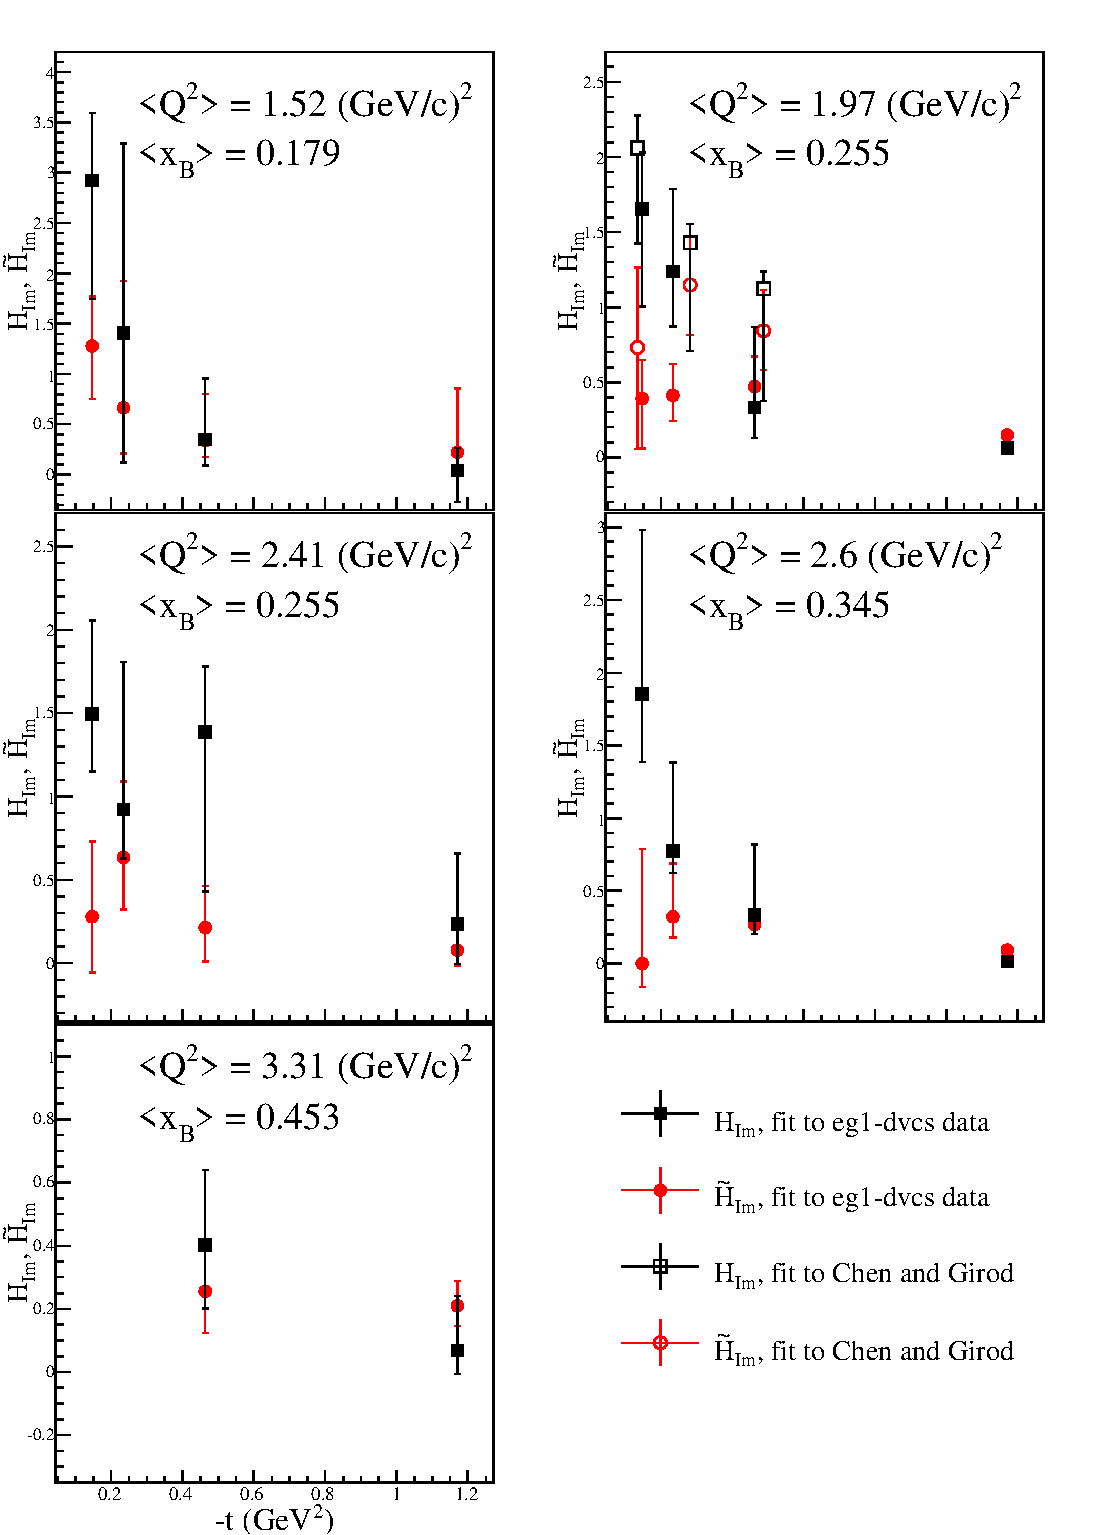
\includegraphics[width=120mm]{CFF_comp_prop.pdf}
\caption[$t$ dependence of $H_{lm}$ and $\tilde{H}_{lm}$.]
{$t$ dependence for each $Q^2$-$x_B$ bin of $H_{Im}$ (black squares) and $\tilde{H}_{Im}$ (red circles). The full points are obtained by fitting the eg1-DVCS data (TSA, BSA and DSA) \cite{pisano}. The empty points were obtained by fitting the BSA results from \cite{fx} integrated over all values of $Q^2$ at $x_B \sim 0.25$, and the TSAs from \cite{shifeng}.}
\label{cffs_eg1dvcs}
\end{center}
\end{figure}

\section{Experimental situation}\label{sec_exp_situation}
The determination of all the GPDs is clearly a non-trivial task, and requires measurement of several observables on both proton and neutron targets. 
Such a dedicated experimental program, concentrating on a proton target, has started worldwide in the past few years. 
Table~\ref{dvcs_exp_summary} summarizes the current situation.  It is evident that while data exist for all proton observables, neutron DVCS data is woefully lacking.  The only existing nDVCS experiment was performed in Hall A \cite{malek}, where the beam-polarized cross section difference was extracted, albeit with small kinematical coverage, low statistical precision, and high systematic uncertainties. There also exists a number of approved 12 GeV pDVCS experiments at JLab, both in Hall A and Hall B, but only one approved neutron experiment, to measure the beam-spin asymmetries using CLAS12 \cite{proposal}.  While the new pDVCS experiments will greatly increase both the coverage and statistics of the existing proton data, we propose to further advance the nDVCS program by performing the first ever measurements of target-spin and double-spin asymmetries on a longitudinally polarized neutron target.

\begin{savenotes}
\begin{table}[t]
   \centering
   \begin{tabular}{|c||c|c|c|} 
\hline
Observable & Sensitivity & Completed & 12-GeV \\
(target) & to CFFs & experiments & experiments \\
\hline
\hline
    $\Delta\sigma_{beam}$(p) & $\Im{\rm m}{\cal H}_p$ & Hall A \cite{carlos},\cite{E07007}\footnote{Analysis underway.}, CLAS \cite{hs} &   Hall A \cite{E1206114}, CLAS12 \cite{E1206119}\\ 
& & &Hall C \cite{E1213010}\\

\hline
    BSA(p)     &    $\Im{\rm m}{\cal H}_p$       & HERMES \cite{hermes}, CLAS \cite{stepan,fx,pisano}   & CLAS12 \cite{E1206119} \\
\hline 
   TSA(p)   &    $\Im{\rm m}\widetilde{\cal H}_p,\Im{\rm m}{\cal H}_p,$     &  HERMES \cite{hermes}, CLAS \cite{shifeng,erin,pisano} & CLAS12 \cite{E1206119}\\
\hline 
    DSA(p)    &    $\Re{\rm e}\widetilde{\cal H}_p,\Re{\rm e}{\cal H}_p$     &  HERMES \cite{hermes}, CLAS \cite{pisano}& CLAS12 \cite{E1206119}\\
\hline 
    tTSA(p)    &    $\Im{\rm m}{\cal H}_p,\Im{\rm m}{\cal E}_p$               &  HERMES \cite{hermes} &  CLAS12 \cite{E1212010}\\
\hline
    $\Delta\sigma_{beam}$(n)    &    $\Im{\rm m}{\cal E}_n$       &  Hall A \cite{malek},\cite{E08025}\footnotemark[\value{footnote}] & \\
\hline
    BSA(n)    &    $\Im{\rm m}{\cal E}_n$       &   & CLAS12 \cite{proposal}\\
\hline
   \end{tabular}
   \caption[Summary of existing and proposed DVCS experiments]
   {Summary of all existing data on proton and neutron DVCS spin observables, along with their sensitivity to the various GPDs. The ``t'' prefix indicates transversely polarized target.}\label{dvcs_exp_summary}
\end{table}
\end{savenotes}

The currently approved CLAS12 program includes about 120 days of beam time allocated for data taking on unpolarized proton target, 120 days on longitudinally polarized proton target (NH$_3$), 90 days on unpolarized deuterium target, and 50 days (plus 15 of overhead) on longitudinally polarized deuterium target (ND$_3$). Considering that the polarization of the deuteron (and of the neutron) in ND$_3$ is about half that of the proton in NH$_3$, that the cross section for neutron-DVCS is more than a factor of two smaller than the one for proton-DVCS, and that the detection efficiency for neutrons is at least a third of that for protons, as of today there is a big difference in statistical power between the polarized proton and neutron datasets for CLAS12. Doubling the current statistics on (ND$_3$), as this proposal aims to do, would contribute to reducing this gap. 

\section{Proposed experimental setup}\label{setup-section}
A dynamically polarized ${}^{14}$ND$_3$ target, described in the next Section, will provide the polarized neutrons on which the 11-GeV polarized electron beam from the upgraded CEBAF will be rastered.
In order to map the complex kinematic dependence of the GPDs, a wide acceptance detector is necessary. For this experiment, we plan to use the CLAS12 detector (Fig.~\ref{clas12}), which will be devoted to the detection of the electron, the neutron (in the Central Neutron Detector, described in Section \ref{cnd-section}) and the DVCS-BH photons. The CLAS12 acceptance for photons reaches down to polar angles of about $5^{\circ}$ with the Electromagnetic Calorimeter (EC). 
The possibility of extending the acceptance for photons down to $2.5^{\circ}$ using the electromagnetic calorimeter of the Forward Tagger (FT) \cite{batta} has been studied (Section \ref{ft_section}). As the results of these studies, which are not fully conclusive at this stage, show potential problems for the use of the FT at full luminosity, it will be used for a subset of the experiment (10 days), with half of the current. This will choice will be motivated and clarified in Section \ref{ft_section}. 
\begin{figure}
\begin{center}
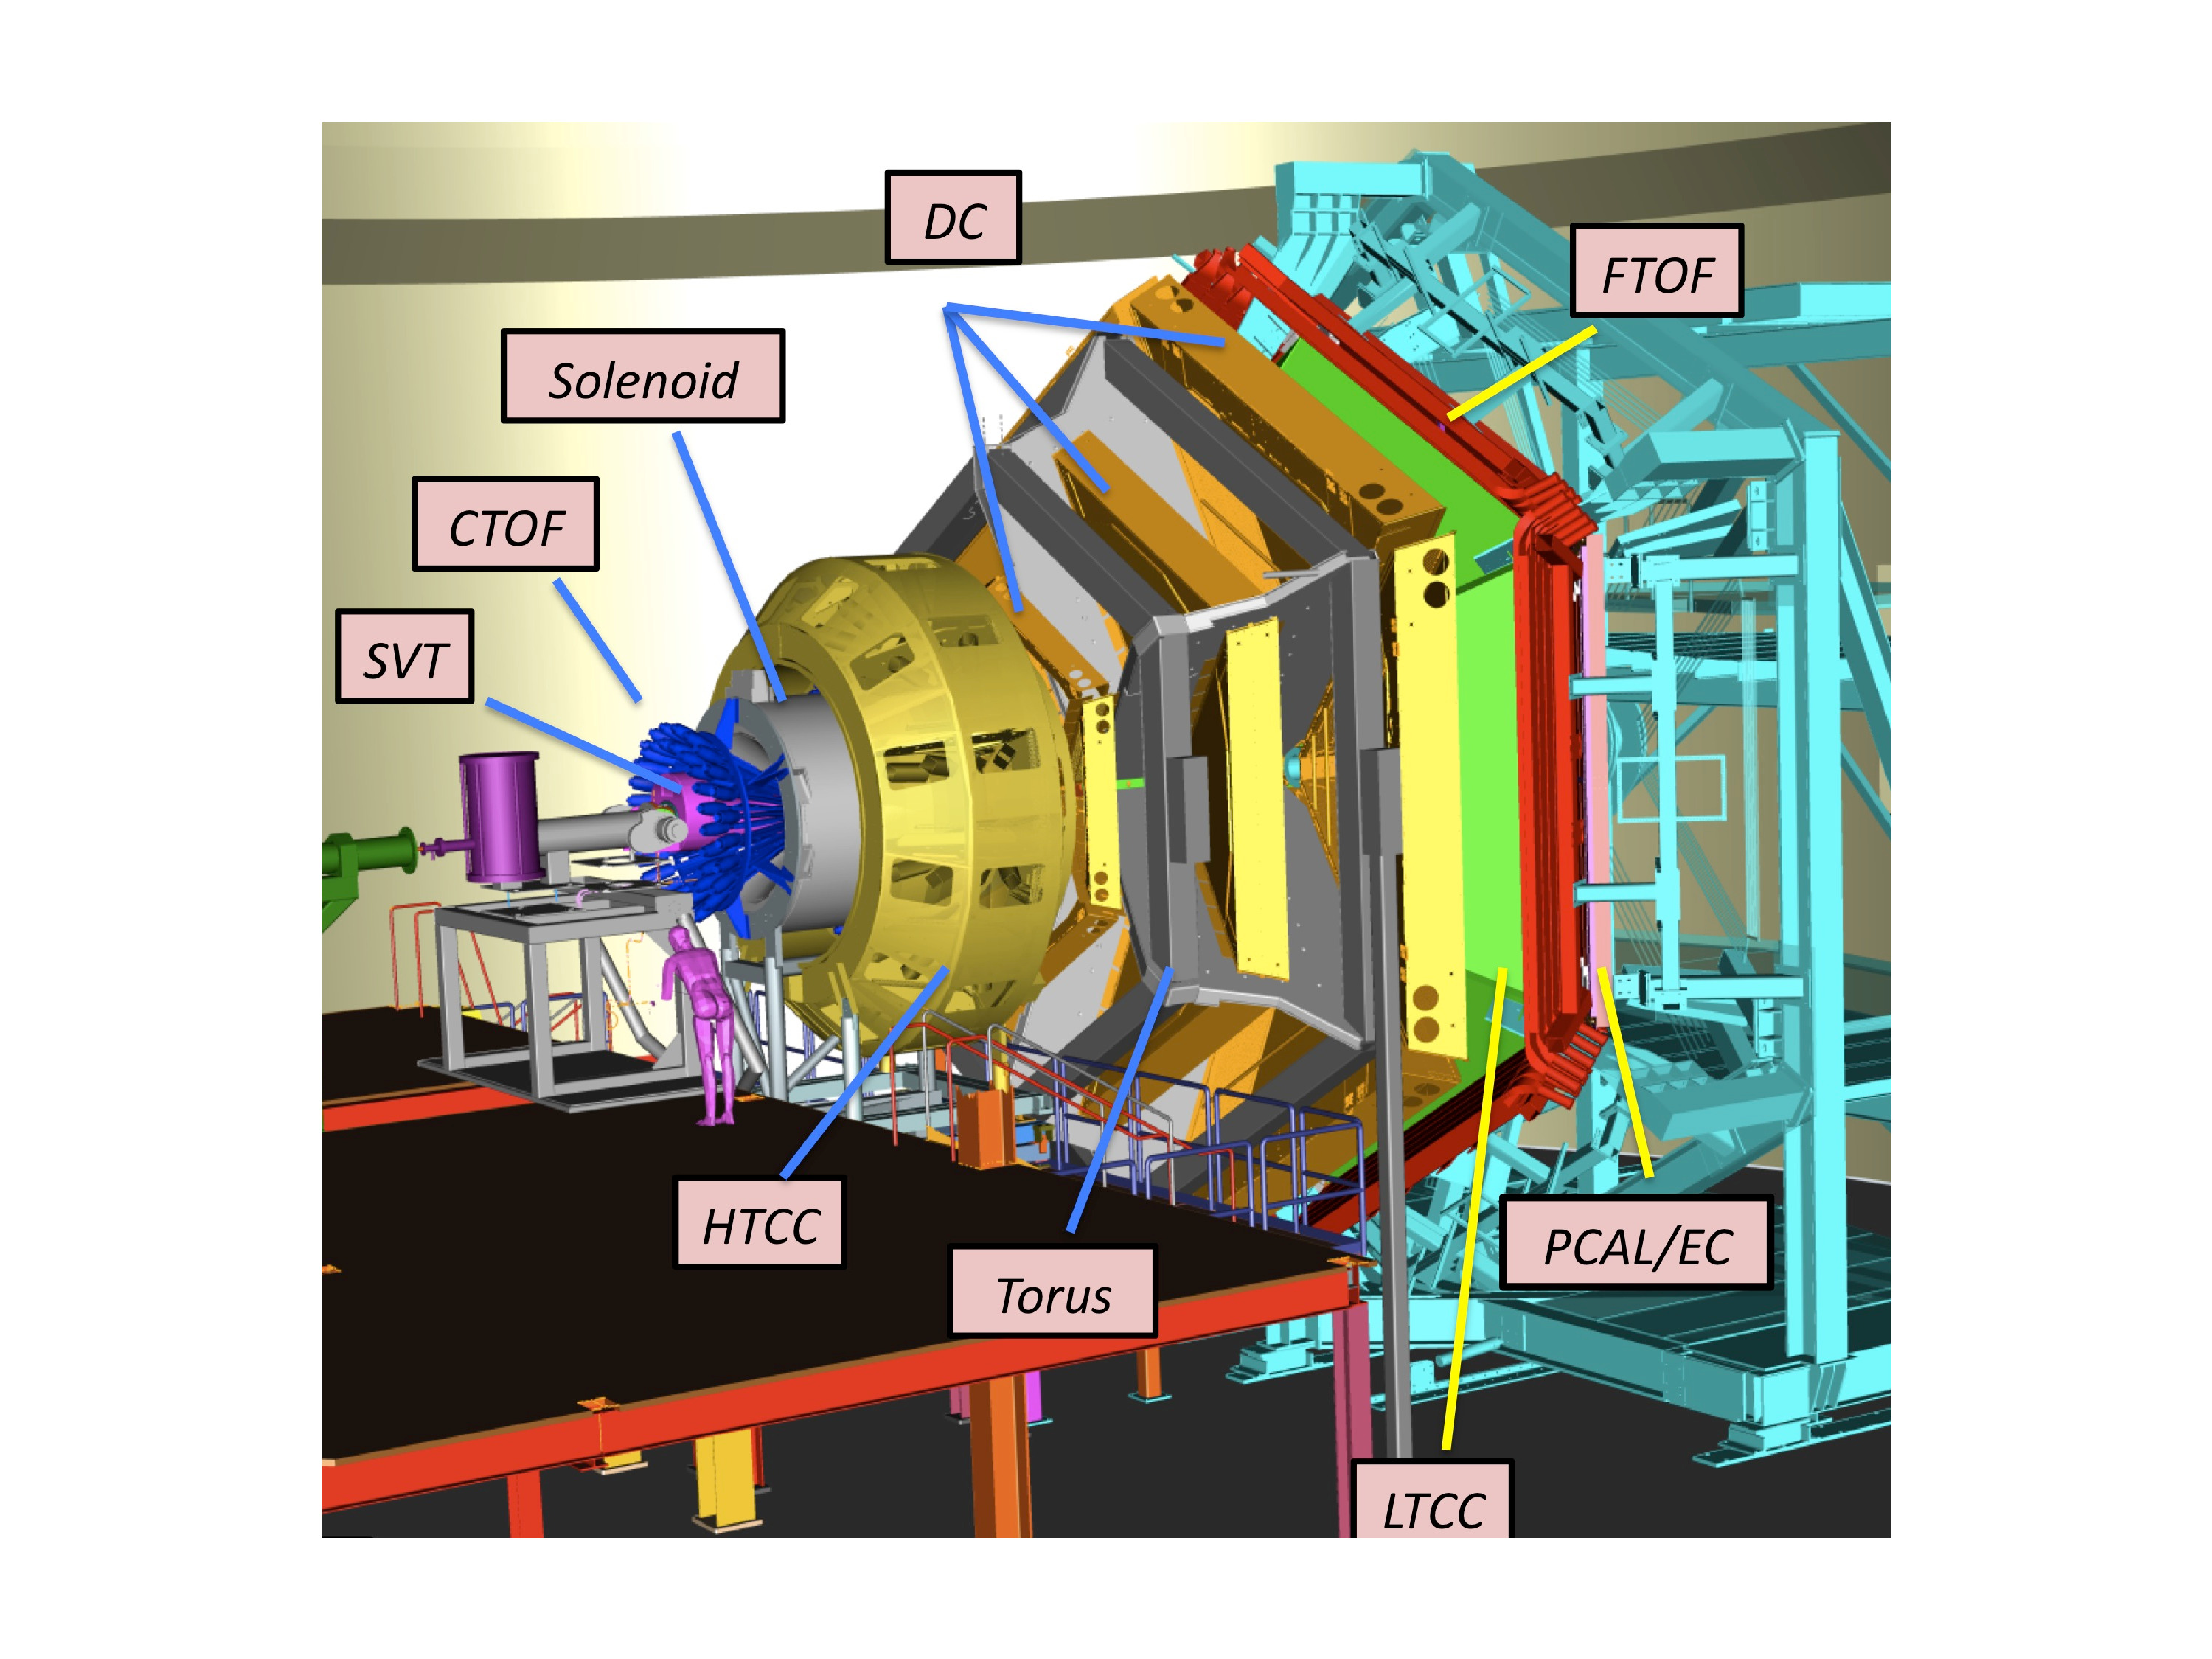
\includegraphics[width=130mm]{clas12-design.pdf}
\caption [The CLAS12 detector and its components]
{The CLAS12 detector and its components. In the forward part, the six coils of the superconducting toroidal magnet segment the detector into six sectors, each equipped with three regions of drift chambers (DC), High- and Low-Threshold Cherenkov Counters (HTCC and LTCC), Pre-Shower and Electromagnetic Calorimeters (PCAL and EC) and Forward Time-of-Flight (FTOF) scintillators. The central detector surrounds the target and is contained inside a solenoid magnet; its base equipment is composed of the Silicon Vertex Tracker (SVT) and the Central Time-of-Flight (CTOF).}
\label{clas12}
\end{center}
\end{figure}


\subsection{Polarized target}\label{poltar-section}
\begin{figure}
\begin{center}
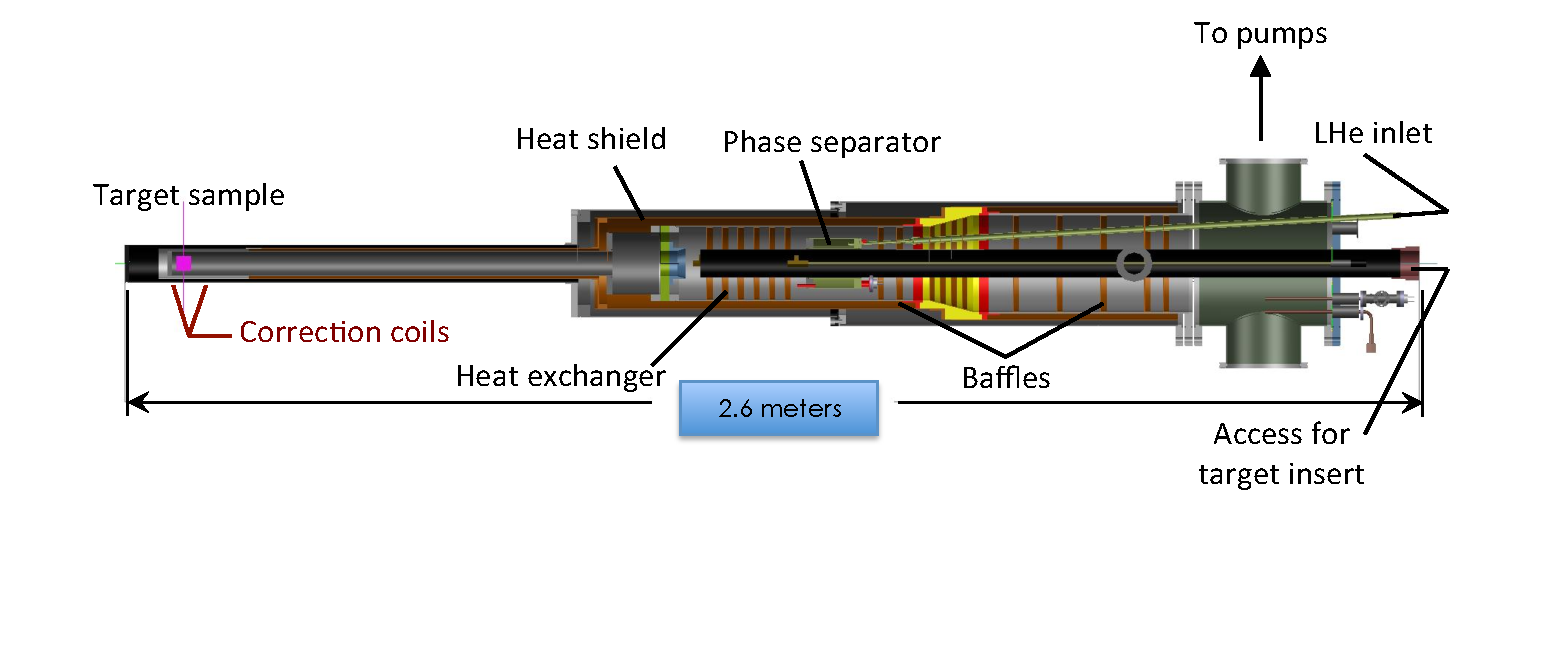
\includegraphics[width=5.5in]{Target_Side.pdf}
\end{center}
\caption{Side view of the CLAS12 dynamically polarized target.}
\label{Target}
\end{figure}
The proposed experiment will utilize a new, dynamically polarized target under construction for the CLAS12 spectrometer by a collaboration of the Jefferson Lab Target Group, the University of Virgina, Old Dominion University and Christopher Newport University.  The target cryostat, shown schematically in Figure~\ref{Target}, is specifically designed according to the geometrical constraints imposed by the CLAS12 detector package, primarily the Silicon Vertex Tracker.  Frozen, deuterated ammonia has been chosen as the target material for its high deuteron content (30\% by weight), high deuteron polarization (up to 50\%), and high resistance to radiation damage \cite{Goertz2002}.  Construction of the target is currently underway, with initial tests anticipated in 2017.

To realize Dynamic Nuclear Polarization (DNP), a dielectric solid is doped with a small concentration 
($10^{19}$~cm$^{\minus3}$) of paramagnetic radicals.  The unpaired electrons in the radicals are highly polarized by cooling the sample to a low temperature and applying a strong magnetic field.  For example, at the proposed operating conditions of 1~K and 5~T, the electron polarization is greater than 99.99\%.  Off-center microwave saturation of the electron spin resonance drives mutual electron/nuclear spin flips which effectively transfer the electron polarization to the nuclei.  Either positive or negative nuclear polarization can be realized, depending on whether the microwave frequency is slightly below or above the electron resonance frequency of 140~GHz.

The target sample will be cooled to 1~K by a bespoke $^4$He evaporation refrigerator with an anticipated cooling power of about 0.5~W at 1.0~K.  The CLAS12 solenoid shall provide the necessary 5~T magnetic field.  For optimum polarization, the uniformity of the field should be about 100 ppm or better over the volume of the sample.  If the solenoid is unable to provide this level of uniformity, it may be necessary to include small superconducting correction
coils inside the target cryostat, or to reduce the sample dimensions.  

\subsubsection{Luminosity}\label{sec_luminosity}
The nominal length of the target container will be $L=4.0$~cm, with a 2.5~cm diameter. 
It will be filled with mm-sized granules of frozen $^{14}$ND$_3$ with a density $\rho =$ 1.007 g/cm$^3$ and a packing fraction $f\approx0.6$.  The total luminosity with electron beam intensity $I$ will be 
\begin{eqnarray}
	\mathcal{L}  & = & f \rho L N_A I   \\
& = & 0.6(1.007\, {\rm g/cm}^3)(4.0\,{\rm cm})(6.02\times10^{23}\,{\rm g}^{\minus 1})(6.24\times10^9\,{\rm s}^{-1}{\rm nA}^{\minus 1}) \nonumber \\
	                   & = & 9.1 \times 10^{33} \, {\rm cm}^{\minus 2} \,{\rm s}^{\minus 1} \,{\rm nA}^{\minus 1} \nonumber
\end{eqnarray}
Note that this number is per nA of incident beam current.  
The luminosity for scattering from polarized neutrons
within the deuterons will be $3/20$ of the above number, or 
$1.4 \times 10^{33}\,{\rm cm}^{\minus 2} \, {\rm s}^{\minus 1} \, {\rm nA}^{\minus 1}$.
We anticipate running most of the experiment at 10~nA, giving a neutron luminosity of $1.4\times10^{34} 
\,{\rm cm}^{\minus 2} \, {\rm s}^{\minus 1}$.  An additional 10 days using the Forward Tagger will be run at a reduced beam current of 5~nA.  In order to reduce effects due to localized beam heating and radiation damage, the beam will be continuously rastered over 2.4~cm of the 2.5~cm target diameter.


\subsubsection{Polarization measurement}\label{sec_target_polarization}
The deuteron polarization will be monitored online by continuous wave NMR, using the industry standard
Liverpool Q-meter \cite{Court1993}.    There are two means whereby the polarization can be extracted from the NMR signal: the area method and the peak-height method.  We intend to use both, and either should provide a relative uncertainty $\Delta P/P \approx 4$\%.  We also intend to extract the polarization offline using the
quasi-elastic scattering asymmetry.

First, the total area of the NMR absorption signal is proportional to the vector polarization of the sample, and the constant of proportionality can be calibrated against the polarization of the sample measured under thermal equilibrium (TE) conditions.  This is the standard method used for polarized proton targets, but can be more problematic for deuteron targets.  Typical conditions for the TE measurements are 5~T and 1.4~K,
where the deuteron polarization is only 0.075\%, compared to 0.36\% for protons.
This smaller polarization, along with quadrupolar broadening, makes the deuteron TE signal more difficult to measure with high accuracy.
We therefore intend to implement a straightforward modification to the NMR circuit that has been shown to improve the stability and signal-to-noise ratio of the NMR signal~\cite{Court2004}. This modification was 
successfully utilized during the eg1-DVCS experiment in Hall B.  

Second, the deuteron polarization can also be extracted from the {\em shape\/} of the NMR signal.  
The deuteron is a spin-1 nucleus with three magnetic substates, $m=\minus1, 0, \plus1$, and the 
NMR absorption signal is a superposition of the $\minus 1-0$ and $\plus 1-0$ transitions.
In the case of ${}^{14}$ND$_3$, the deuteron's electric quadrupole moment interacts with electric field gradients within the molecule and splits the degeneracy of the two transitions.  The degree of splitting depends on the 
angle between the magnetic field and direction of the electric field gradient.  The resultant line shape, integrated over a sample of many polycrystalline beads, has the form of a Pake doublet (see Fig.\/\ref{NMR}).  
It has been experimentally demonstrated that, at or near steady-state conditions, the magnetic substates of deuterons in dynamically polarized ${}^{14}$ND$_3$ are populated according to the Boltzmann distribution with a characteristic {\em spin\/} temperature $T_s$ that can be either positive or negative, depending on the sign of the polarization. In this case, the vector polarization can be determined by the
ratio of the two transition intensities, $r=I_{\plus} / I_{\minus}$ \cite{Dulya1997}:
\begin{equation}
P_z = \frac{(r^2-1)}{(r^2 + r +1)}.
\end{equation}
An online estimate of the polarization can be made by comparing the heights of the two peaks.  
For a more accurate determination, an offline analysis of the entire line shape is necessary \cite{Dulya1997}.

\begin{figure}
\begin{center}
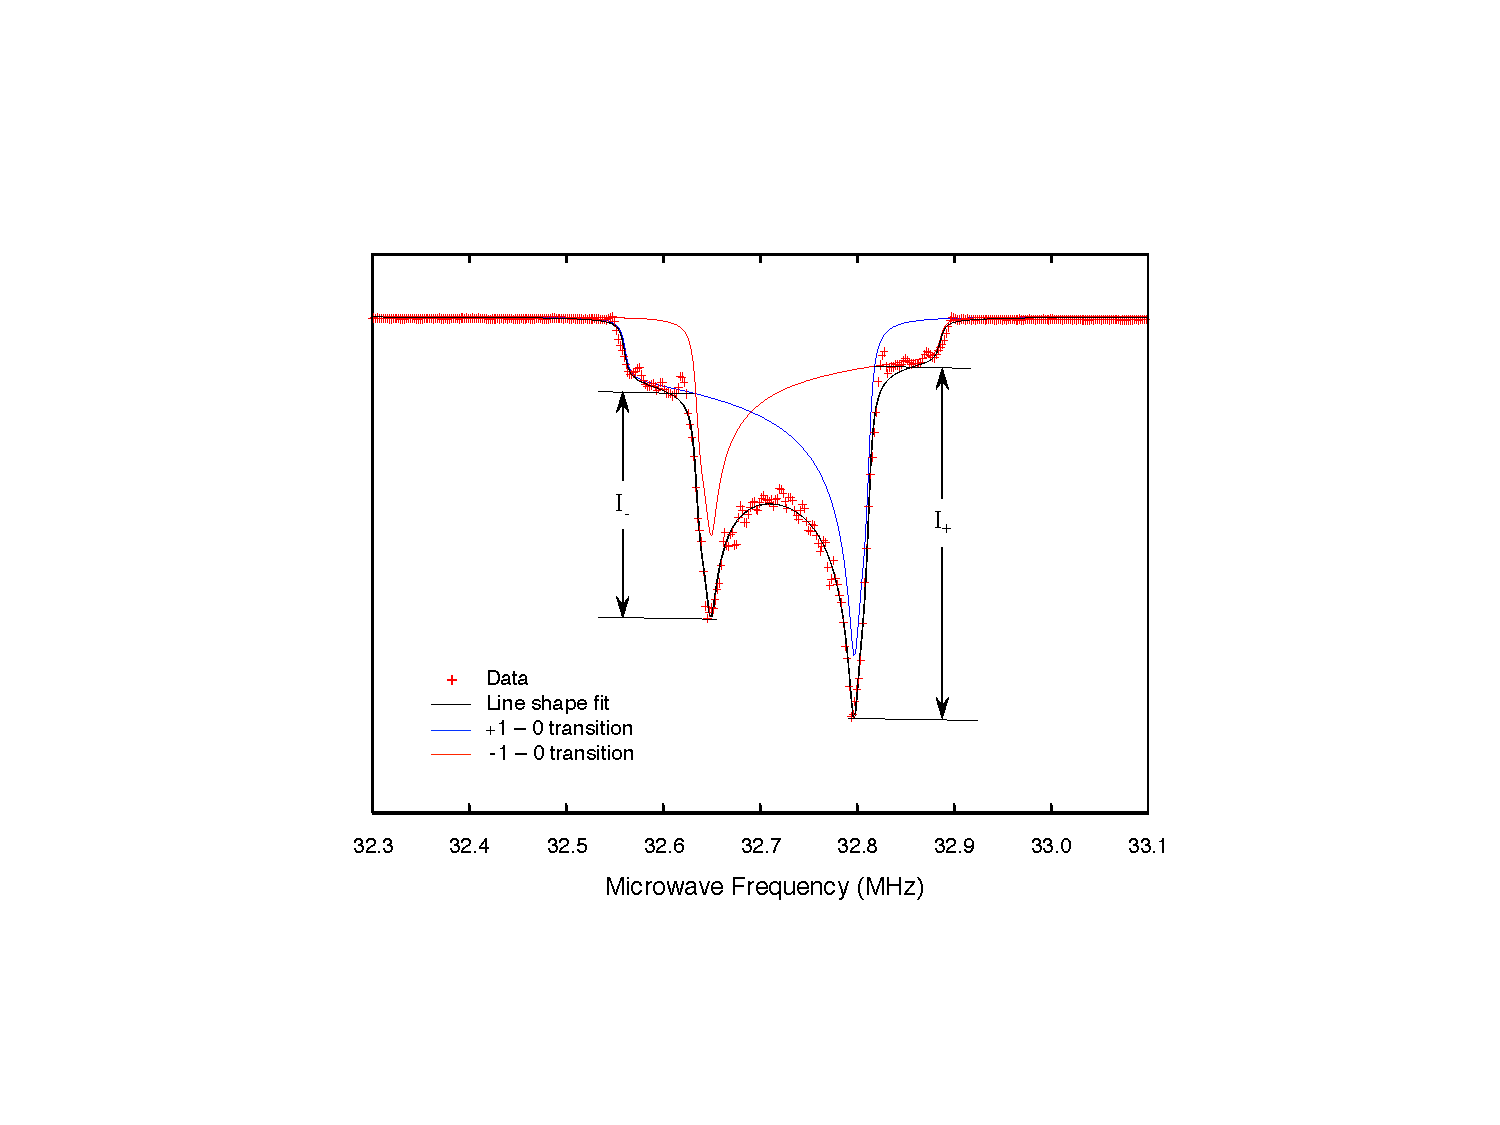
\includegraphics[width=3in]{Stache_NMR.pdf}
\end{center}
\caption[Typical ${}^{14}$ND$_3$ NMR signal]
{Typical NMR signal of polarized ${}^{14}$ND$_3$.  The black line results from a sophisticated line shape 
analysis of the data points and is a superposition of the two NMR transitions shown in red and blue.
This figure is adapted from~\cite{Kwaltine2013}.}
\label{NMR}
\end{figure}

Finally, the polarization will also be studied offline using the experimental data. We will extract the product of the beam and target polarization, $P_b P_t$, by measuring the quasi-elastic asymmetry ($\vec{d}(e,e'p)$) and by comparing it with the known theoretical value:
\begin{equation}
  P_b P_t=\frac{1}{D_f}\frac{A_{meas}}{A_{theo}}
\end{equation}
where $D_f$ is the dilution factor to account for the contribution of the unpolarized background (Section~\ref{sec_dilution}).
The target polarization value, needed for the TSA, will be then computed by taking the ratio of $P_bP_t$ and  the value of the beam polarization $P_t$, measured in dedicated M{\o}ller polarimetry runs. 

\subsubsection{Overhead for target operation}\label{sec_target_over}
There are four routine target operations that must be considered as overhead. 
First, we intend to provide an initial dose of approximately 20~Pe$^{\minus}$/cm$^2$ at 200~nA to each target sample prior to its use in the nDVCS experiment.\footnote{1 Pe$^{\minus} = 10^{15}$ electrons.}  This is necessary to achieve the highest possible deuteron polarization, as is explained below.  Second, the target must be periodically warmed to approximately 100~K in order to repair the deleterious effects of radiation damage, a process known as annealing.  Third, the target sample must be replaced when the anneals become ineffective at repairing the radiation damage.  Fourth, the NMR system will be periodically calibrated by performing
measurements of the thermal equilibrium polarization of deuterons at 5~T and temperatures around 1.4~K.
We examine each of these in the following sections, and a summary is made at the end.
Note that most overhead operations do not require the CEBAF electron beam, and are 
therefore counted as calendar days, not PAC days (one calendar day = two PAC days).
The only exception is the initial cold dose of electrons, as described below. Please note that this overhead estimate is for the total 110 days of beam time, consisting of 50 already-approved days and the additional 60 requested in this proposal. The target overhead is about the same for each. 

\vspace{-.15in}
\paragraph{Cold dose:}
In solid ammonia, paramagnetic radicals are created within the target sample by ionizing radiation, usually 
in the form of a 10--20~MeV electron beam, at a dose of about 
100~Pe$^{\minus}$/cm$^2$.
This is usually applied with the material cooled to 90~K with liquid argon, after which it may be stored indefinitely in liquid nitrogen.  
In the case of {\em deuterated\/} ammonia, experience has shown that polarizations greater than 20\% are only achieved after an additional  ``cold'' dose of approximately 10~Pe$^{\minus}$/cm$^2$ 
has been applied to the sample at 1~K.  
During the EG4 program in Hall B, the deuteron polarization increased from an initial value under 20\% to more than 45\%  after a cold dose of  20~Pe$^{\minus}$/cm$^2$~\cite{Slifer2007}.  In this case, the CLAS detectors were turned off and a 100~nA beam was applied to the sample for an hour or so, followed by a 100~K anneal.  These cold irradiations were interspersed with normal data-taking at 2~nA, and the deuteron polarization was observed to increase after each anneal, eventually exceeding 45\%.  Rather than following this prescription, we intend to prepare each target sample with a 20~Pe$^{\minus}$/cm$^2$ cold dose before using it in the experiment.  The CLAS12 detectors will be turned off for this procedure, which will require about a day for each sample at 200~nA. 

\vspace{-.15in}
\paragraph{Annealing:}
As a solid polarized target material, deuterated ammonia has a remarkably high resistance to radiation damage, 
exceeded only by lithium hydride and lithium deuteride.
When exposed to ionizing radiation, the decay of the polarization is roughly exponential in manner,
\begin{equation}
  P = P_o e^{-D/\delta}.
\end{equation}
Here $D$ is the dose, measured in Pe$^{\minus}$/cm$^2$.
The critical dose $\delta$ of ND$_3$ is different for the positive and negative spin states, with
$\delta_{\plus} = 13$~Pe$^{\minus}$/cm$^2$ and
$\delta_{\minus} = 26$~Pe$^{\minus}$/cm$^2$~\cite{Goertz2002}.
The polarization decay is due to the creation of additional paramagnetic species
that do not contribute directly to the DNP process, but do contribute to the spin-lattice 
relaxation of the nuclear spins.
Fortunately, the concentration of these new radicals can be reduced by annealing the target sample at temperatures up to about 100~K for some tens of minutes.

For the purposes of this proposal, we assume an initial polarization of 45\%, 
which has been achieved in both the Hall C polarized target and the original Hall B
polarized target.  To maintain an average polarization of 40\%, the radiation 
damage must be repaired by annealing the target sample when the polarization 
falls to 35\%, or in other words, when the dose reaches 
$\minus \ln(\frac{0.35}{0.45})\delta \approx 5$~Pe$^{\minus}$/cm$^2$.  
Here we have used the average value of $\delta_{\plus}$ and $\delta_{\minus}$.  
Assuming a 10~nA beam current distributed evenly over a 2.4~cm diameter, 
this dose will be accumulated, on average, after 4 days.  We estimate a total of four
hours will be required to anneal the target, cool it back to 1~K, and repolarize it to 40--45\%.

\vspace{-.15in}
\paragraph{Target lifetime:}
During 100 days of beam time at 10~nA, the polarized target
will accumulate a total dose of 120~Pe$^-$/cm$^2$, while an additional 10 days at 5~nA will deposit
6~Pe$^-$/cm$^2$.
However, the maximum that a ND$3$ sample can tolerate before it must be replaced is not fully known.  
McKee~\cite{McKee2004} reports that for the Gen01 experiment in Hall C, a total of dose of
315~Pe$^{\minus}$/cm$^2$ was deposited on six different samples, and at least one continued to give high polarizations even after a dose of 100~Pe$^{\minus}$/cm$^2$.  The total dose had little or no effect on the frequency of anneals, although the maximum attainable polarization did decline slightly after about 
50~Pe$^{\minus}$/cm$^2$.   For this proposal we make the conservative estimate that the samples will be replaced after a total dose of 50~Pe$^{\minus}$/cm$^2$, of which 20~Pe$^{\minus}$/cm$^2$
will occur before data-taking begins.  The remainder will be incurred after about
25~days of data-taking at 10~nA, and so we anticipate that four samples of ND$_3$ will be sufficient 
for the entire experiment, with one sample incurring an additional 6~Pe$^-$/cm$^2$ 
for the Forward Tagger runs.  Dedicated carbon runs will occur between the ND$_3$ sample changes.
The time required to replace an old ND$_3$ sample with the carbon target, then replace the carbon with fresh
ND$_3$, perform a TE calibration on the new sample and polarize it to 40--45\% should be about 12 hours. Note that this does not include the actual time spent acquiring data on the carbon target.

\vspace{-.15in}
\paragraph{TE measurements:}
Thermal equilibrium (TE) measurements are necessary to calibrate the NMR system,
and must be performed whenever a new target sample is introduced into the experiment.  Additional
measurements are made throughout the experiment in order to monitor and reduce sources of systematic uncertainty such as gain drift and settling of the sample beads.   
To perform a TE, the target sample must first have its existing dynamic polarization destroyed, either by temporarily warming the sample or temporarily lowering the magnetic field to zero.  The sample must then be allowed to achieve its thermal equilibrium polarization, which it approaches in an exponential manner with a spin-lattice time constant $T_1$ that depends on the field strength, the sample's temperature, and its density of paramagnetic radicals. Since annealing the sample reduces its radical density and increases $T_1$, 
it is best to do TEs prior to the anneals.  Most measurements are made around 1.4~K, where the signal size is not too small, and $T_1$ is not too long.
Because the deuteron TE signal is small, a significant amount of signal averaging must be utilized to achieve a precise determination of its area, and so the time required for each measurement will depend strongly on the signal-to-noise ratio of NMR system.  Based on past experience, we assume six hours will be sufficient.  This includes the time required to polarize the sample to 40-45\% at the end of the calibration.

\vspace{-.15in}
\paragraph{Target overhead summary:}
Based on the above information we provide the following estimate for the total overhead necessary to operate the polarized target.  The total is about 8 PAC days.  Whenever possible, anneals, TE measurements, and target changes can be coordinated with scheduled or unscheduled beam outages to lessen their impact on data acquisition and further reduce the overhead.  
%One possible sequence is indicated in Fig.~\ref{Operation}.
%\begin{figure}[ht]
%\begin{center}
%includegraphics[width=5.in]{Operation.pdf}
%\end{center}
%\caption[Possible target operation sequence]
%{One possible sequence of target operations for the 80 day experiment. The numbers indicate the total dose accumulated during data taking, in Pe$^-$/cm$^2$. The experiment ends after 95~Pe$^-$/cm$^2$.
%{\bf CD}: Cold Dose.  {\bf TE}: Thermal Equilibrium measurement.  {\bf A}: Anneal. }
%\label{Operation}
%\end{figure}
\begin{enumerate}
  \item{Cold dose of 20~Pe$^{\minus}$/cm$^2$ at 200~nA.  Required: 4 @ 24 hours each. 
    Total: 96 PAC hours.}  
    \item{Anneal every 5~Pe$^{\minus}$/cm$^2$.  Required: 22 @ 4 hours each. 
      Total: 88 calendar hours = 44 PAC hours.}
      \item{Change target sample after 30~Pe$^{\minus}$/cm$^2$.  Required: 3 @ 12 hours each.  
      Total: 36 calendar hours = 18 PAC hours.}
        \item{TE calibration of NMR system at the beginning of each target sample, and after 
          15~Pe$^{\minus}$/cm$^2$.  Required: 12 @ 6 hours each.  
          Total: 72 calendar hours = 36 PAC hours}.
\end{enumerate}

\begin{figure}
\begin{center}
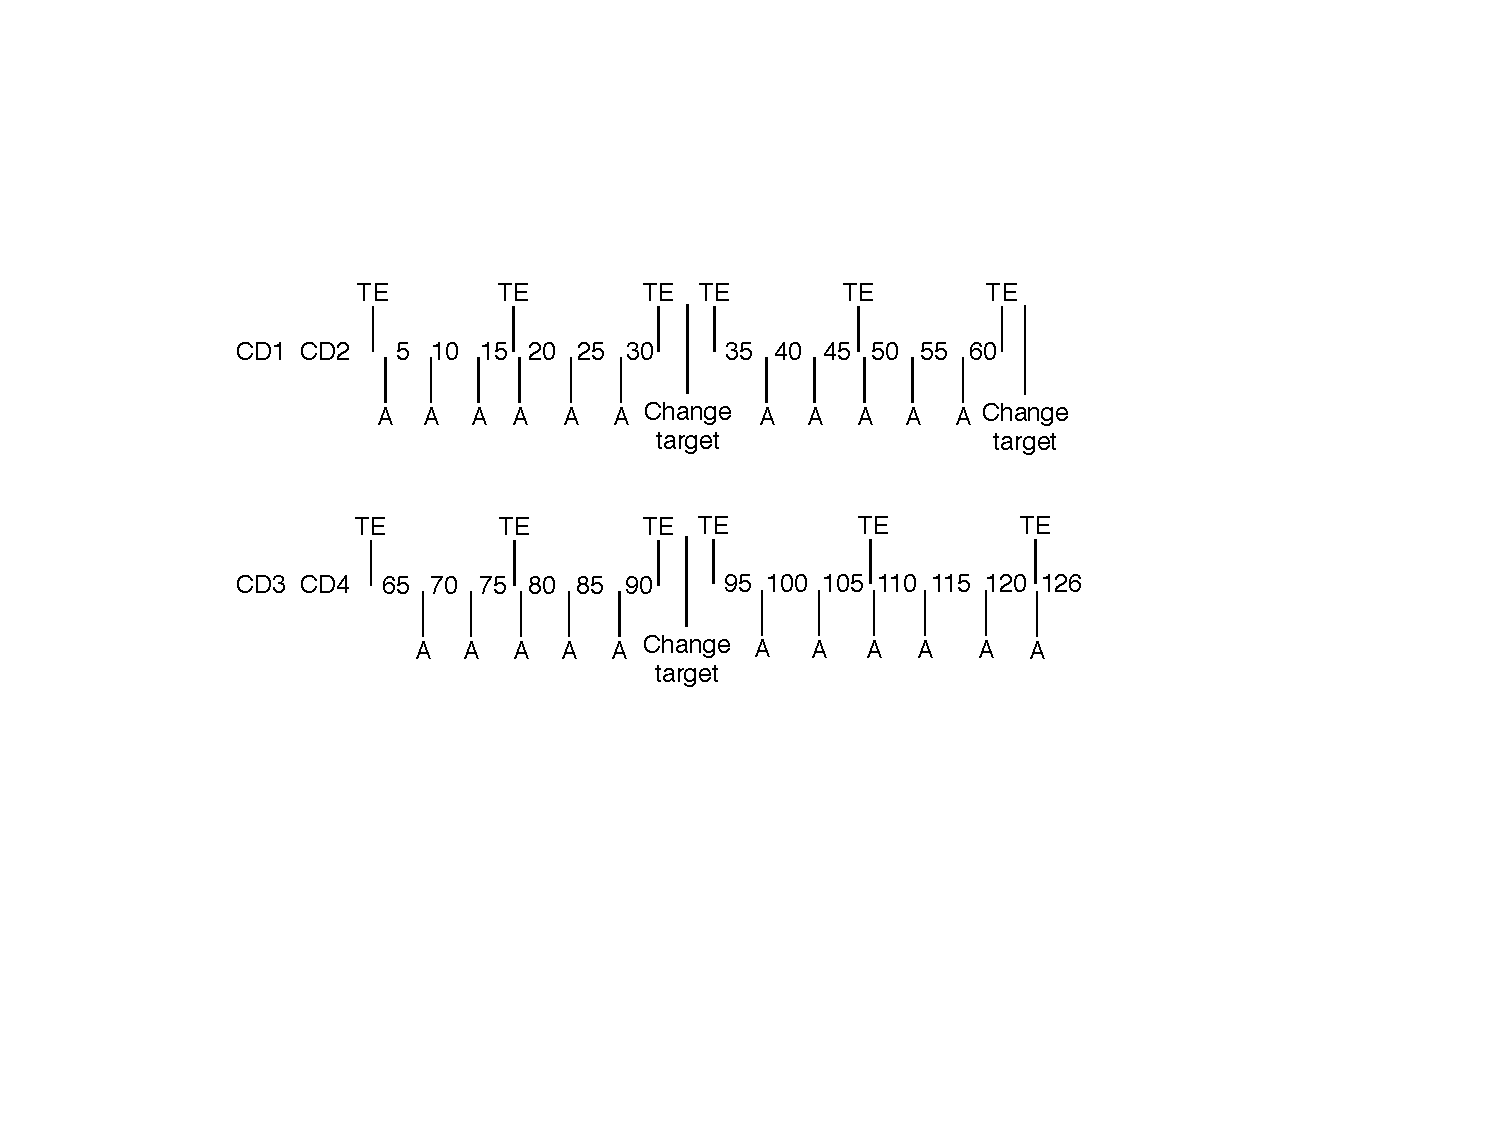
\includegraphics[width=6in]{Operation_110days.pdf}
\end{center}
\caption[Overhead operations of the target]
{One possible sequence of target operations for the entire 110-day experiment. The top half represents the 50 days of already-approved beam time, and the bottom half the 60 days of extension. The numbers indicate the total dose accumulated during data taking, in Pe$^-$/cm$^2$. The experiment ends after 126 Pe$^-$/cm$^2$. 
{\bf CD:} Cold Dose. {\bf TE:} Thermal Equilibrium measurement. {\bf A:} Anneal.}
\label{Operation}
\end{figure}


\subsection{Central Neutron Detector}\label{cnd-section}
The Central Neutron Detector was conceived to extend the CLAS12 acceptance for the recoil neutrons of nDVCS, which are expected to be mostly emitted between $50^{\circ}$ and $70^{\circ}$ \cite{proposal}. The requirements of the detector are:
\begin{itemize}
\item{good capabilities for neutron identification, via the measurement of $\beta$ (with $\beta=\frac{v}{c}$), for the kinematic range of interest ($0.2<p_n<1.2$ GeV/c, $40^o<\theta_n<80^o$)} and
\item{neutron momentum resolution $\sigma_P/P$ within 10\%,}
\end{itemize}
Early simulation studies \cite{proposal} showed that these performances can be achieved by a scintillator-based detector providing a timing resolution of about 150 ps. 

\begin{figure}[ht]
\begin{center}
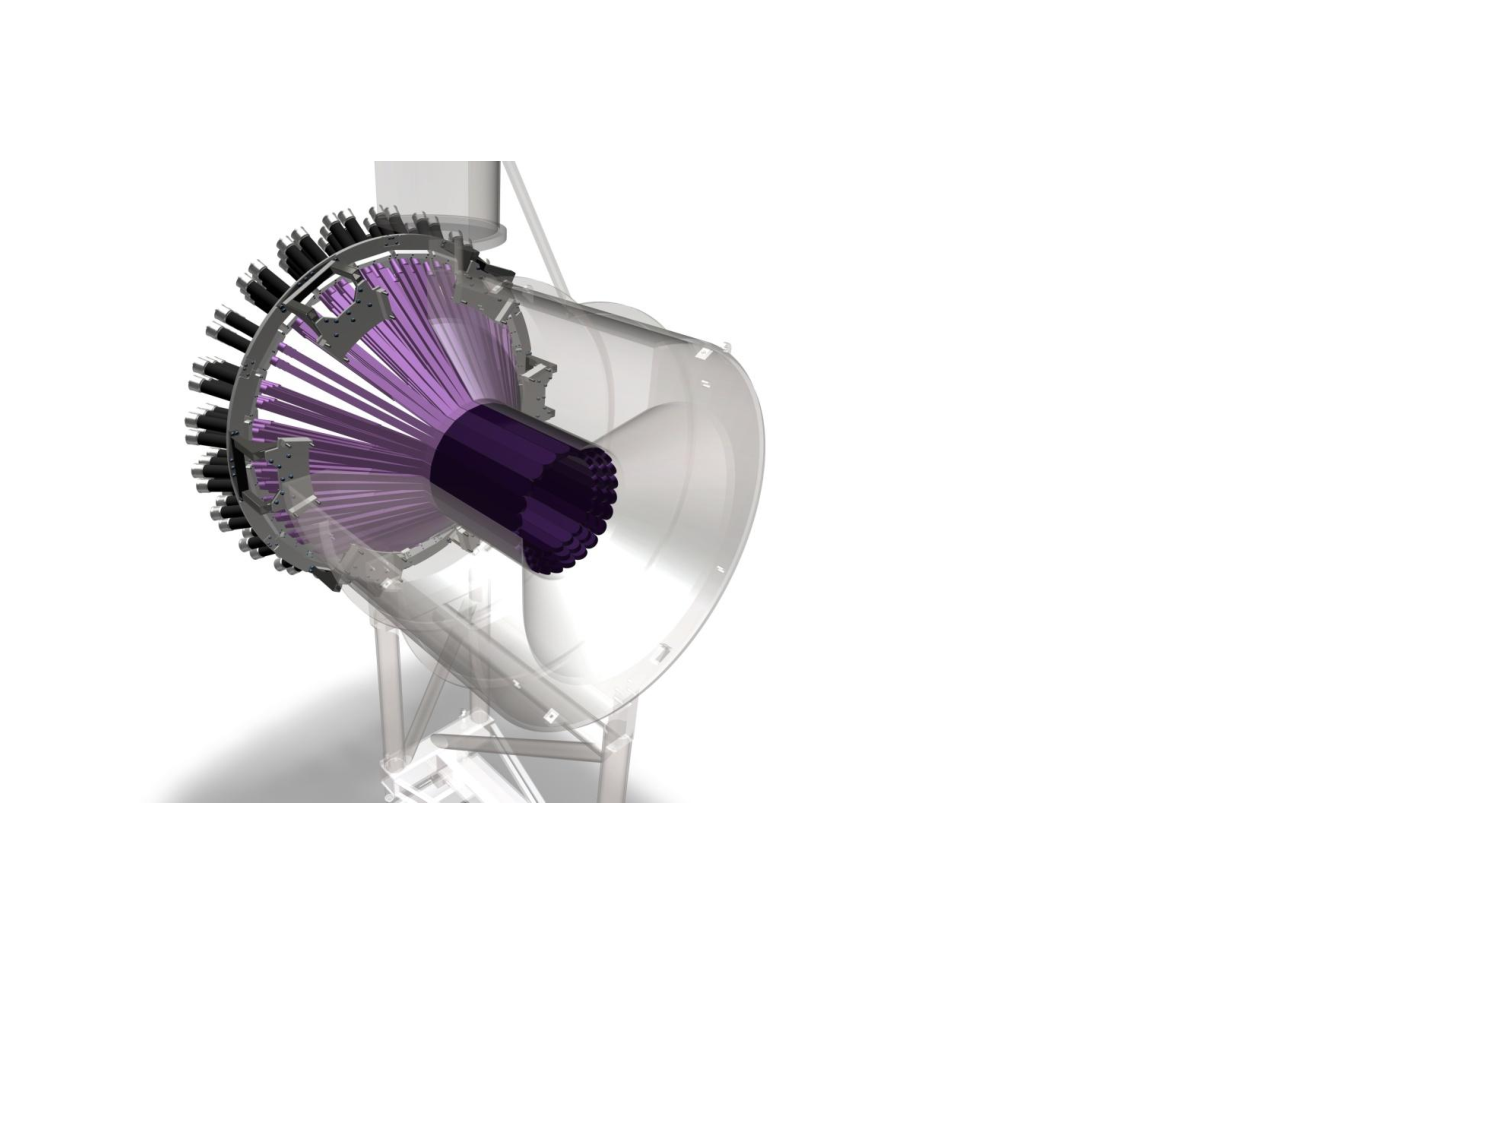
\includegraphics[width=3.5in]{CND_bello.pdf}
\end{center}
\caption [Design of the Central Neutron Detector]
{Design of the Central Neutron Detector, inserted in the CLAS12 solenoid.}
\label{cnd_nice}
\end{figure}

The core of the CND (Fig.~\ref{cnd_nice}), which will be placed in the Central Detector, in the 10 cm of radial space left between the Central Time Of Flight (CTOF) and the solenoid magnet, is a barrel, coaxial with the beam direction, made of three radial layers of trapezoidal plastic-scintillator bars. 
Each radial layer contains 48 bars, connected in pairs by a "u-turn" light guide at the downstream end.
Photomultipliers are coupled to the upstream end of each scintillator via 1.5m-long light guides. For each hit, half of the light emitted in a scintillator paddle is collected by the upstream PMT (the ``direct'' signal), while the other half propagates through the u-turn and the neighboring paddle to the PMT connected at its end (the ``indirect'' signal). 

Three such scintillator pairs (inner, middle, and outer) are grouped together to form a single, radial "block".  The CND comprises 24 of these blocks, covering the entire azimuthal range (Fig.~\ref{CND_Orsay}).

\begin{figure}
\begin{center}
    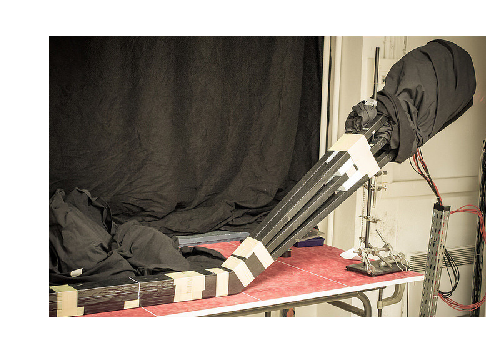
\includegraphics[height=40mm]{block_tested_2.pdf}
    \includegraphics[height=40mm]{cnd_finito.jpg}
  \caption{Construction and testing of the CND at Orsay. Left: one 2x3 block undergoing cosmic ray tests.  Right: all 24 blocks installed into a mock-up of the CLAS12 solenoid.}
  \label{CND_Orsay}
\end{center}
\end{figure}
The assembly of the CND, which was entirely carried out at the IPN Orsay, started in December 2013, and was completed in February 2015. The detector was shipped and stored at JLab in June 2015, awating its installation in CLAS12. Upon assembly, each block of the CND was tested with cosmic rays, triggering on the triple-coincidence of the signal in all three layers. Data were taken for about one week for each block, and the block performances were studied, with special attention to the timing resolution. 
Figure~\ref{tdc_adc_raw} shows the raw distribution of TDCs as a function of ADCs for the six PMTs in one of the 24 blocks. Notice the clear separation between direct (low-TDC/high-ADC) and indirect (high-TDC/low-ADC) signals. 

To define an average time resolution for our setup in the triple-coincidence trigger configuration, we use the method inspired by the work done in \cite{giles} and later adopted for the CLAS TOF system \cite{elton_paper}. 

\begin{figure}
\begin{center}
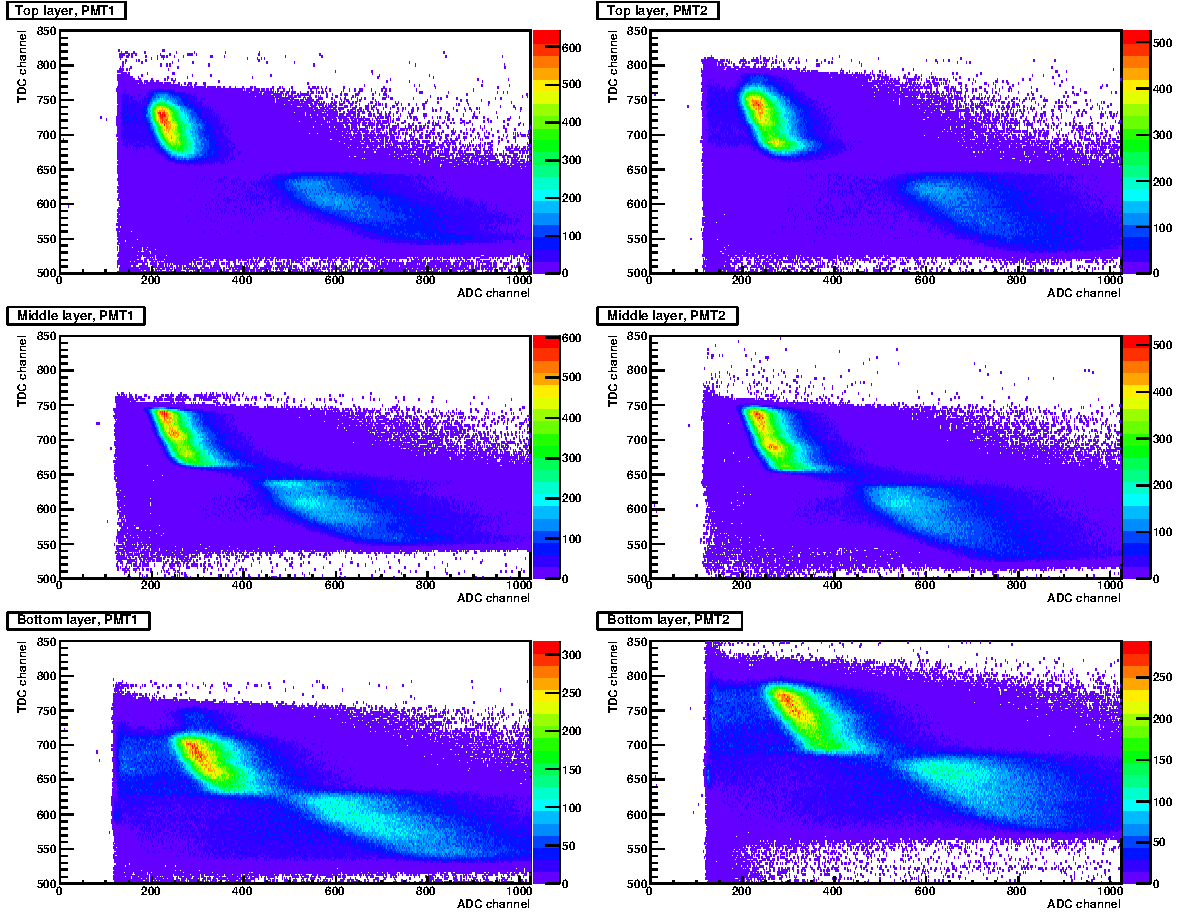
\includegraphics[width=140mm]{tdc_adc_raw.pdf}
\caption[Cosmic ray data for the CND]
{Cosmic rays data. Raw TDC vs ADC for each of the six PMTs of block 2 of the CND. No pedestal subtraction or data-cleaning cuts are applied.}
\label{tdc_adc_raw}
\end{center}
\end{figure}

\begin{figure}
\begin{center}
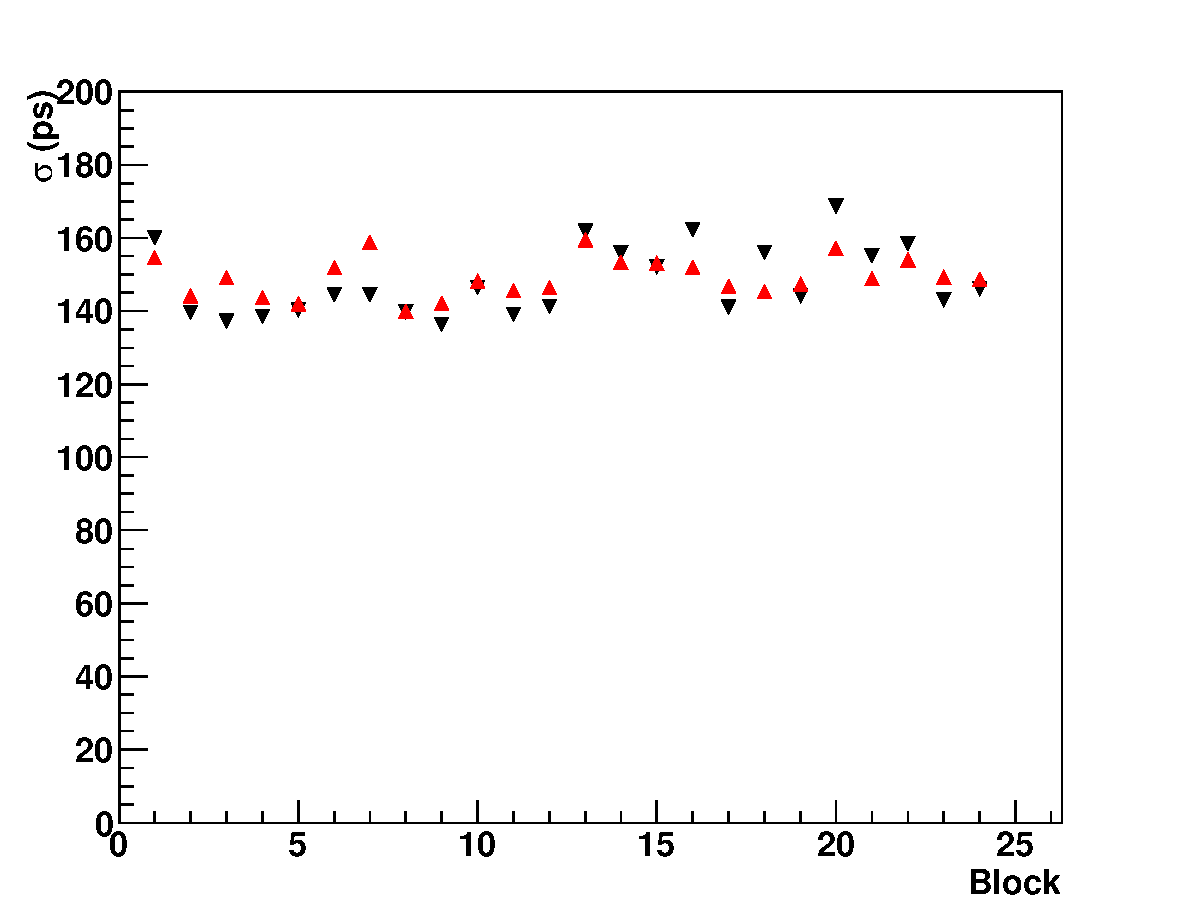
\includegraphics[width=80mm]{res_blocks.pdf}
\caption[Time resolution of the CND]
{Average time resolution for each block of the CND from cosmic rays measurements in triple-coincidence. The black and red triangles are the results obtained with the formulae from, respectively, Refs.~\cite{elton_paper} and \cite{vitali}.}
\label{res_blocks}
\end{center}
\end{figure}

The timing resolutions for all the CND blocks, computed according to the method of \cite{elton_paper}, are represented by the black triangles in Fig.~\ref{res_blocks}. The average is 148.0 ps. As a cross check, the resolution was also computed using the method adopted by V. Baturin for the CLAS12 CTOF \cite{vitali} (red triangles in Fig.~\ref{res_blocks}, with average 149.3 ps). The results of the two methods are consistent. The resolutions of the 24 blocks are very close to the required 150 ps. The systematic uncertainty of our results is estimated to be about $7\%$, determined by repeating the measurements multiple times, and by comparing multiple subsets of each measurement. 

Thus, for resolutions of 150 ps, we have a systematic uncertainty of about 10 ps.

It is also worth mentioning that the TDCs that will be used for the actual experiment will have a better resolution (25ps/channel) than the ones used for these tests (50ps/channel).

\subsection{Simulation and reconstruction}\label{sim_sec}
\begin{figure}[htb]
\begin{center}
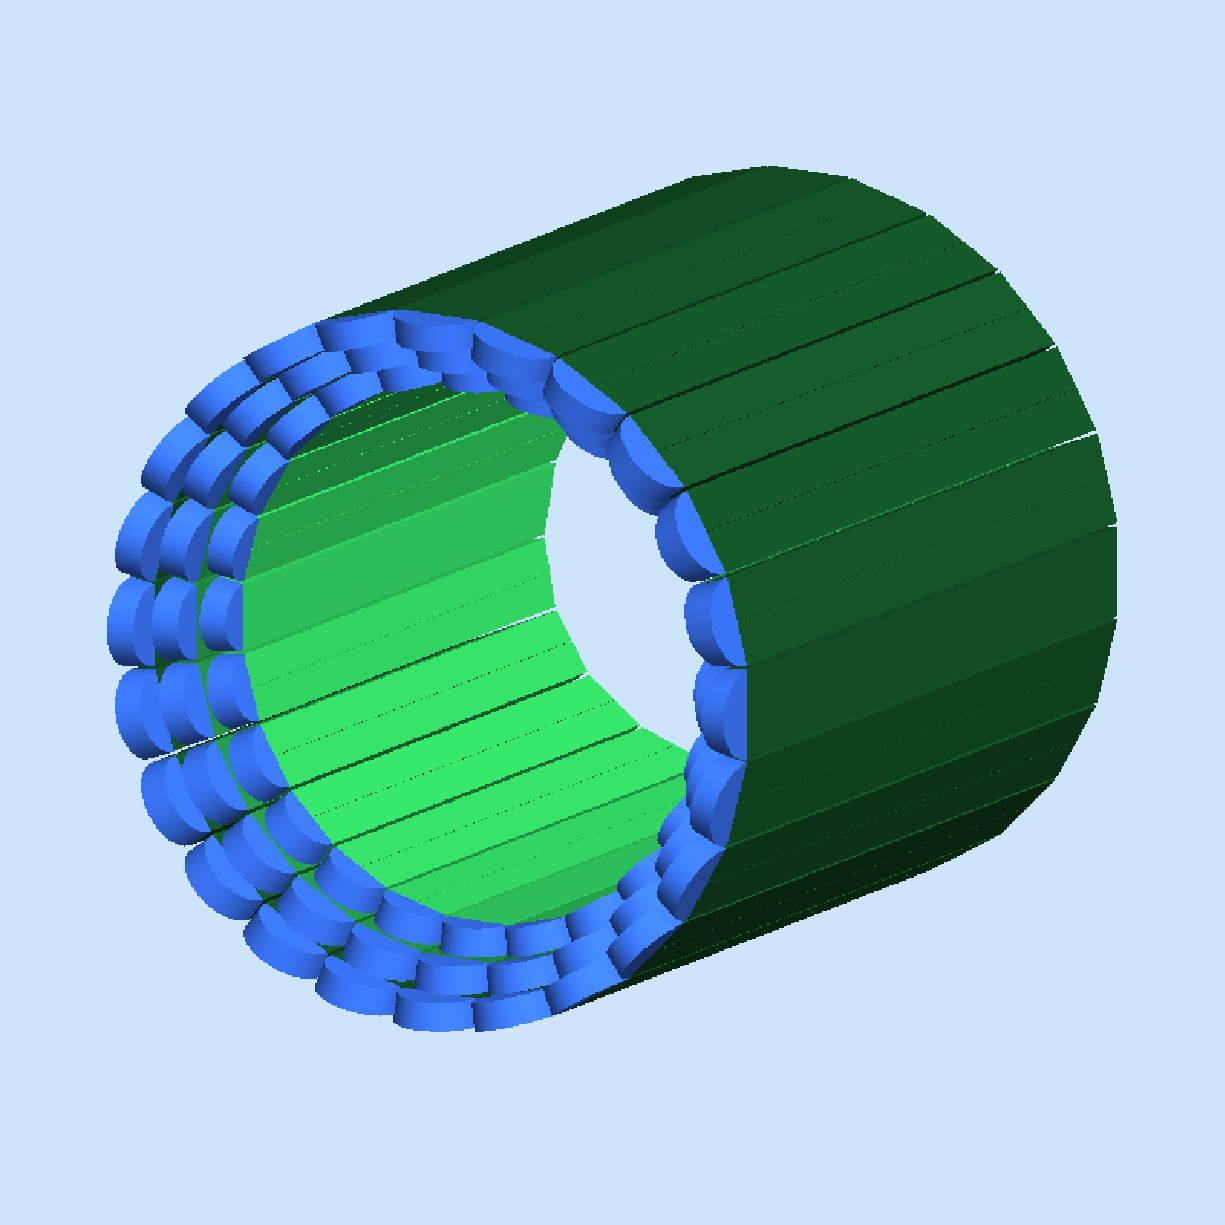
\includegraphics[width=80mm]{CND_4.pdf}
%\vspace{-3.5cm}
\caption {Geometry of the Central Neutron Detector in the GEMC simulation, showing three layers of scintillator paddles (green) coupled in pairs via u-turn light guides (blue) downstream.}
\label{cnd_gemc}
\end{center}
\end{figure}

In order to study the performances of this detector, and thus evaluate the projected results of the nDVCS experiment, its geometry (Fig.~\ref{cnd_gemc}) has been added to the CLAS12 GEANT4-based simulation package, GEMC \cite{mauri}. The energy loss of the particle in the scintillator material is converted to numbers of optical photons in accordance with Birk's formula \cite{birks}, the resulting signal is propagated through the scintillator paddle, light guide and PMT, and the final charge and time are digitized to mimic the output from the ADC/TDC \cite{daria_wiki}.

The timing resolution and the energy loss due to the u-turn geometry have been included in the simulation using the values measured in the cosmic-rays tests described in the previous section. 

Simulations, which included all the other components of the Central Detector, have been run to evaluate the efficiency of the CND for neutrons, its ability to discriminate between neutrons and photons, and its angular and momentum resolutions. Neutrons and photons of momenta varying between 0.1 and 1 GeV/c and having polar angles $\theta$ varying between $50^o$ and $70^o$ have been generated at fixed azimuthal angle ($\phi = 0^o$), pointing to the center of one of the scintillator bars. The results obtained with these simulations are described here below..

\subsubsection{Efficiency}\label{efficiency-section}

 The detection efficiency is defined here as the ratio between the number of events for which a good hit (i.e., a hit having deposited energy above a given threshold) was successfully reconstructed as a neutron in the correct azimuthal bin of the CND and the total number of neutrons generated. 
Several values of energy thresholds, between 1 and 5 MeV, have been tested. 
The efficiency decreases with increasing threshold, and ranges between 12\% at the lowest thresholds and 7\% at the highest ones. 
Figure~\ref{eff_vs_mom} shows the efficiency as a function of the momentum of the neutrons, at a fixed energy threshold of 2 MeV, and for different values of $\theta_n$. 

\begin{figure}[t]  
\begin{center}
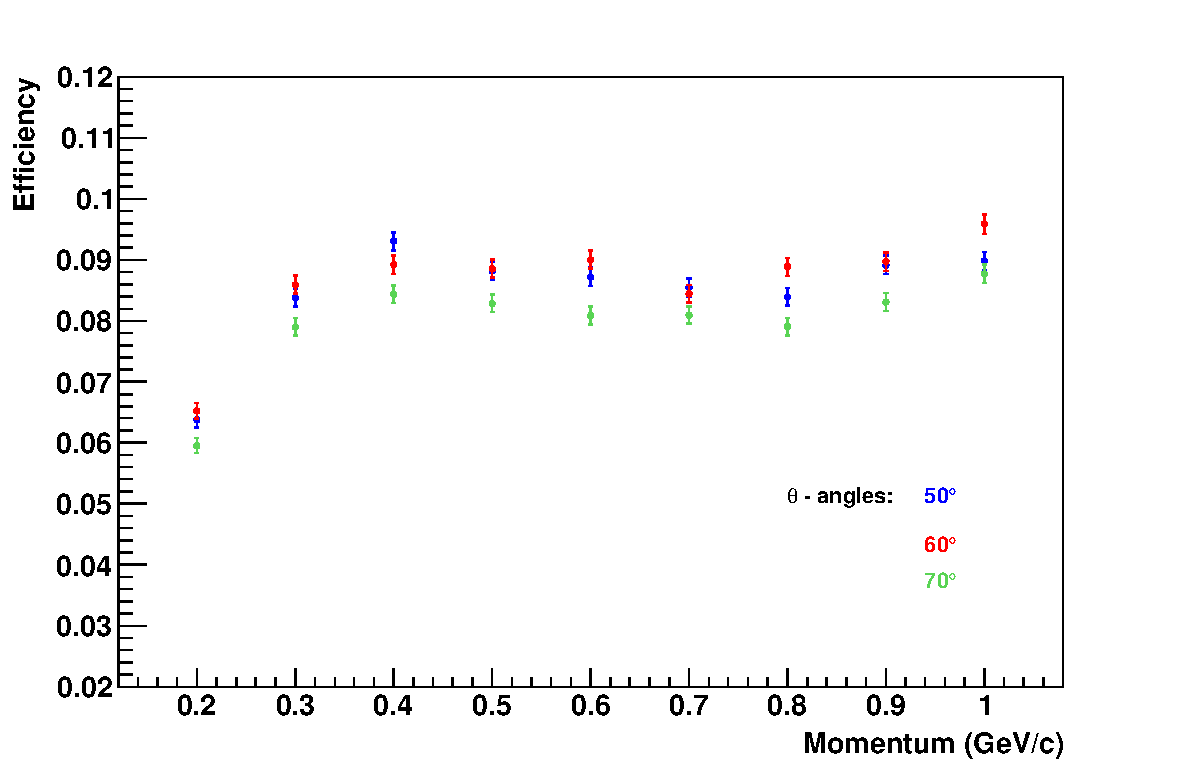
\includegraphics[width=100mm]{eff_vs_mom_diff_theta_II.pdf}
\caption [Neutron detection efficiency as a function of neutron momentum]
{Efficiency for the detection of neutrons, as a function of neutron momentum, for a 2-MeV threshold on the deposited energy. The efficiency is shown for three different values of $\theta_n$, between $50^o$ and $70^o$.
}
\label{eff_vs_mom}
\end{center}
\end{figure}

\subsubsection{Angular and momentum resolutions}\label{resolution-section}

The resolutions on the polar angle $\theta$ of the neutron that can be obtained with the CND are strongly linked to its TOF resolution. The angle $\theta$ is in fact given by
\begin{eqnarray} 
\theta = (180/\pi)\cdot \arccos (\frac{z_{ave}}{l})
\end{eqnarray}
where the reconstructions of the radial distance of the hit from the target, $l$, and of its position along the scintillator bar, $z_{ave}$,  both depend on the time measurement. Using a value deduced from the measurements on the CND prototype to apply a gaussian smearing on the timing \cite{proposal}, 
%\begin{equation}\label{eq_time_smear}
%\sigma_t=\frac{A}{\sqrt{E_{dep}}}, 
%\end{equation}
%(see Appendix~\ref{sec_rec})
the $\theta$ resolution resulting from GEMC was studied as a function of neutron momentum and $\theta$ itself. The results are shown in Fig.~\ref{theta_n_tofcut5}, where the angular resolution $\sigma_\theta$, obtained via gaussian fits of the simulated $\theta$ distributions, is plotted as a function of  $\theta$, for a particular value of neutron momentum (0.4 GeV/c). $\sigma_\theta$ is seen to increase slightly with the angle, from $1.5^{\circ}$ to $3.5^{\circ}$.  It has also been found to be relatively insensitive to the neutron momentum. 

The resolution on the azimuthal angle is directly connected to the total number of scintillator bars along $\phi$. In fact, the bin size $\Delta\phi$ is given by
\begin{eqnarray} 
\Delta\phi = \frac{360^{\circ}}{N}=7.5^{\circ}
\end{eqnarray}
where $N$ is the total number of paddles in $\phi$ (48 for the final design of the CND). $\sigma_\phi$ can be taken as half of $\Delta\phi$, therefore $3.75^o$.
\begin{figure}[hbt]  
\begin{center}
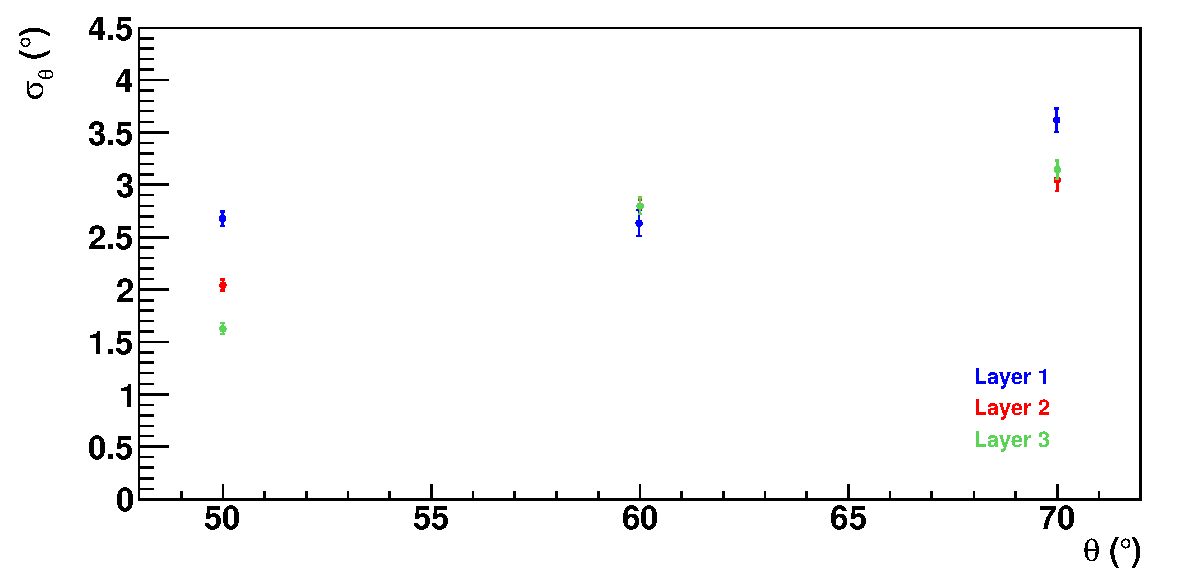
\includegraphics[width=100mm]{sigma_theta_vs_theta_diff_layer.pdf}
\caption [Angular resolution of the CND as a function of $\theta$]
{Angular resolution $\sigma_\theta$ as a function of $\theta$ for neutrons of momentum 0.4 GeV/c, for a 2-MeV threshold on the deposited energy. The three colors of the points correspond to the three radial layers of the CND.}
\label{theta_n_tofcut5}
\end{center}
\end{figure}

\begin{figure}  
\begin{center}
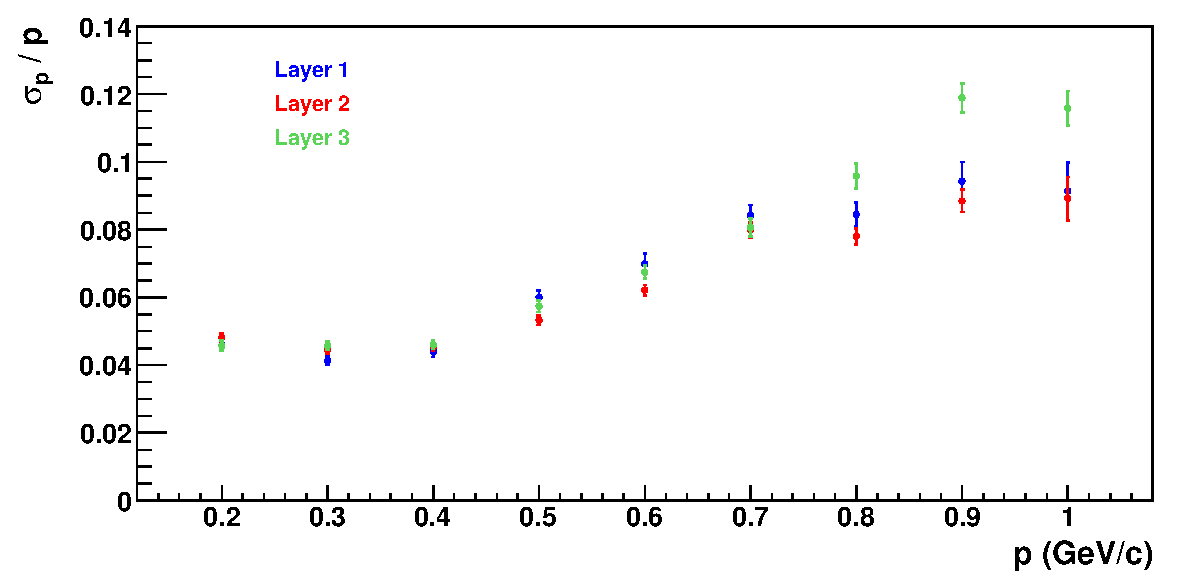
\includegraphics[width=100mm]{mom_res_vs_mom_diff_layers.pdf}
\caption [Momentum resolution as a function of $p$]
{Momentum resolution $\sigma_p/p$ as a function of $p$ for neutrons having $\theta=60^o$, for a 2-MeV threshold on the deposited energy. The three colors of the points correspond to the three radial layers of the CND.}
\label{p_n_tofcut5}
\end{center}
\end{figure}

The resolution on the neutron momentum, calculated after particle identification on the basis of $\beta$, according to the formula
\begin{eqnarray}
p = \frac{\beta\cdot m_n}{\sqrt{1-\beta^2}},
\end{eqnarray}
is also strictly connected to the TOF resolution. Figure \ref{p_n_tofcut5} shows the momentum resolution $\sigma_p/p$ as a function of momentum for neutrons emitted with $\theta=60^o$: it increases with increasing momentum, and ranges between 4\% and 11\%. No appreciable variations of momentum resolution are observed by varying the neutron polar angle.


\subsubsection{Particle Identification}\label{pid-section}

Since the charged particles passing through the CND will be vetoed by the Central Tracker, the only particles that could be mistaken for neutrons in the CND are the photons. 
The efficiency of the CND for detecting photons (Fig.~\ref{eff_photons}) has been estimated in simulations to be similar to that for neutrons, about 10\% for photon energies down to 0.2 GeV.  The efficiency drops to zero for lower energy photons, depending on the threshold cut applied. 

\begin{figure}  
\begin{center}
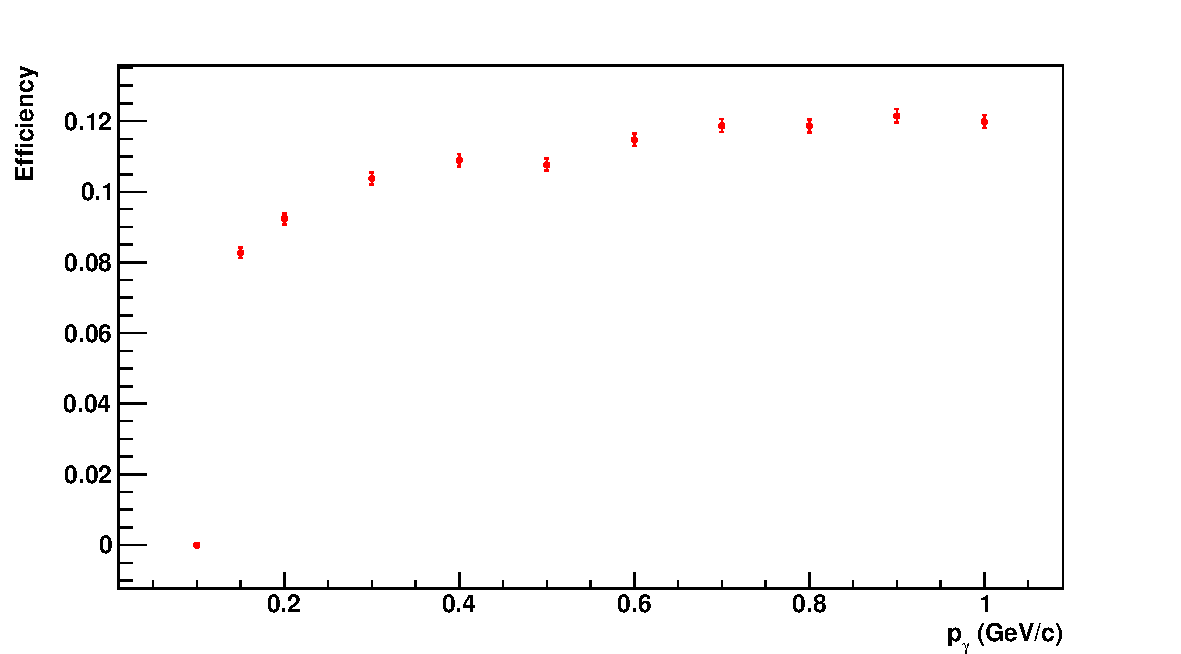
\includegraphics[width=100mm]{efficiency_photons_60deg_new.pdf}
\caption [Photon detection efficiency as a function of photon momentum]
{Efficiency for the detection of photons, as a function of photon momentum, for a 2-MeV threshold on the deposited energy. The efficiency is shown for $\theta_{\gamma}=60^o$. Below $E_\gamma=0.15$ GeV, the photon efficiency drops to zero.}
\label{eff_photons}
\end{center}
\end{figure}

\begin{figure}
\begin{center}
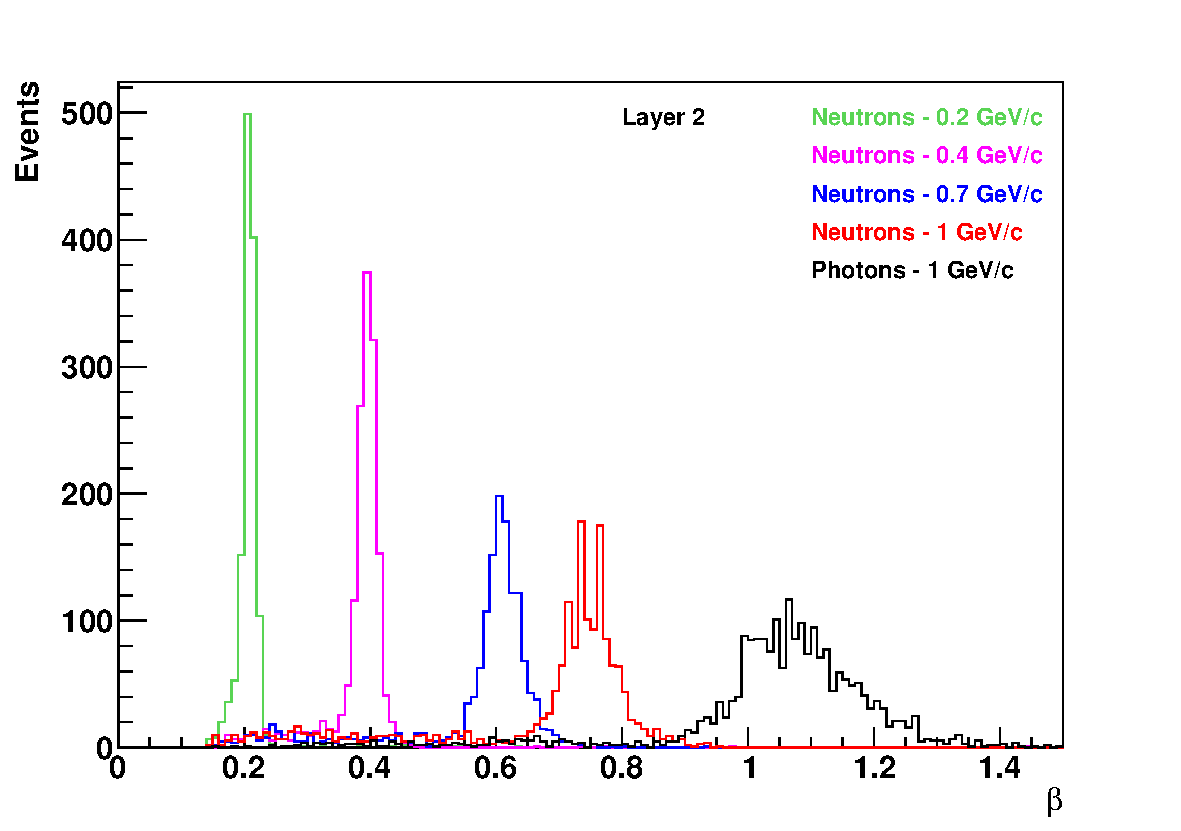
\includegraphics[width=80mm]{beta_comp_layer_2_II.pdf}
\caption [$\beta$ distributions for neutrons and photons in the CND]
{$\beta$ distributions for neutrons with $p_n=0.2$ GeV/c (green), $p_n=0.4$ GeV/c (purple), $p_n=0.7$ GeV/c (blue), $p_n=1$ GeV/c (red), and photons with $E=1$ GeV, for the middle layer of the CND. 
The threshold on the deposited energy is 2 MeV. The plots show all hits, integrated over $\phi$. Equal neutron and photon yields have been assumed here.}
\label{beta_n_g}
\end{center}
\end{figure}

\begin{figure}
\begin{center}
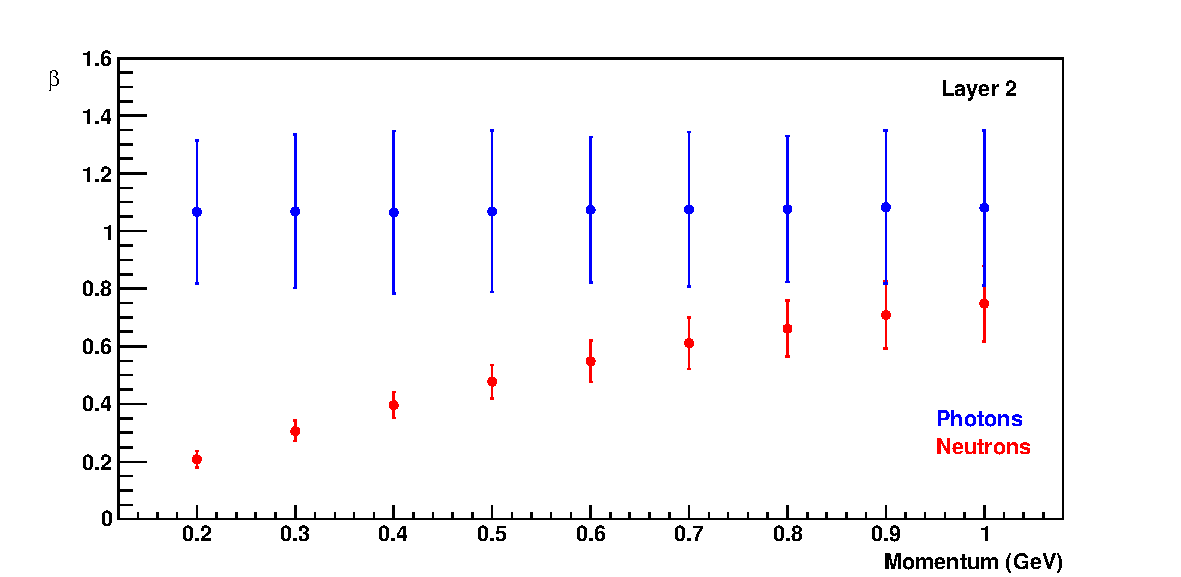
\includegraphics[width=100mm]{beta_res_n_g_comp_L2.pdf}
\caption [$\beta$ versus momentum for neutrons and photons in the CND]
{$\beta$ versus momentum for neutrons (red) and photons (blue) with momenta between 0.2 and 1 GeV, for the middle layer of the CND. The error bars are defined as $3\sigma$, where $\sigma$ is the fitted width of each $\beta$ peak. The threshold on the deposited energy is 2 MeV.}
\label{fig_beta_res}
\end{center}
\end{figure}

Neutrons can be discriminated from photons by means of their $\beta$, and so GEMC simulations have been performed to estimate the $\beta$ distributions that may be obtained from the CND.  Results for one of the three radial layers, integrated over the azimuthal angle, is shown in Figure~\ref{beta_n_g}.  Here $\beta$ distributions for neutrons with momenta between 0.2 and 1 GeV/c are compared with 1 GeV photons.  Very clear separation is evident for neutrons less than about 0.9 GeV/c, which comprise over 90\% of the expected nDVCS events. 

This is evident also from Fig.~\ref{fig_beta_res}, where the error bars correspond to $3 \sigma$, where $\sigma$ is the gaussian width of each $\beta$ distribution. Equal neutrons and photon yields have been assumed for this study. This assumption has been justified with detailed studies on the different types of photonic backgrounds that can affect the CND \cite{proposal}.

\section{nDVCS at CLAS12: kinematics and acceptances}
In order to study the kinematics of the reaction and determine the expected count rates for both the nDVCS signal and its main background ($ed\to en\pi^0(p)$), an event generator for DVCS/BH and exclusive $\pi^0$ electroproduction on the neutron inside a deuterium target has been developed \cite{ahmed}. The DVCS amplitude is calculated according to the BKM formalism \cite{belitski}, where the GPDs have been taken from the standard CLAS DVCS generator \cite{harut}. The Fermi-motion distribution is calculated with the Paris potential \cite{paris}. The exclusive $\pi^0$ electroproduction channel is generated assuming longitudinal dominance within the naive quark model approximation \cite{ahmed}. Note that no smearing effects due to the nuclear ND$_3$ target are included in the event generator. 

The output of the event generator was fed through CLAS12 FASTMC, to simulate the acceptance and resolutions of electrons and photons in the Forward Detector. 

The expected resolutions and acceptance of the CND for neutrons, outlined in the previous sections, were also included in the FastMC code. 

\begin{figure}[t]
\begin{center}
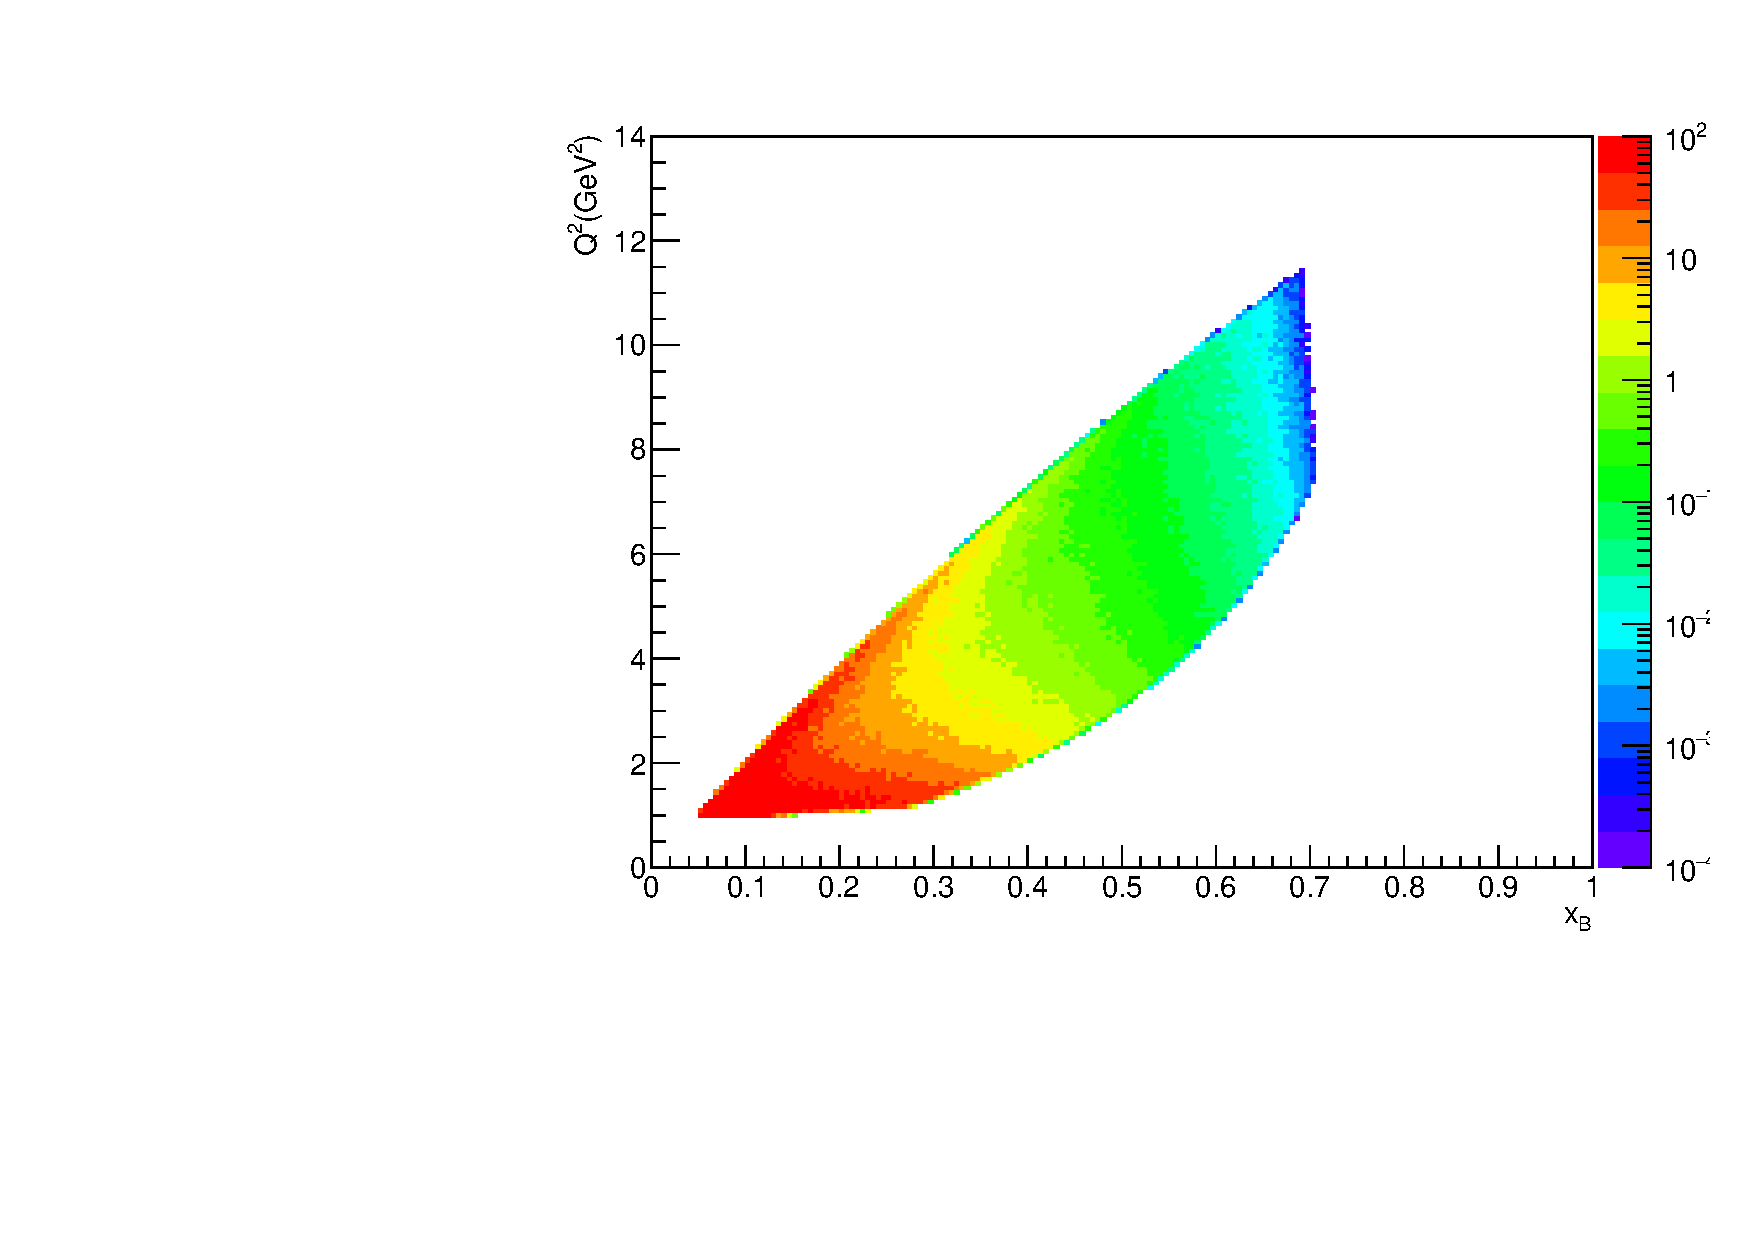
\includegraphics[width=2.9in]{q2vsxb_FT.pdf}
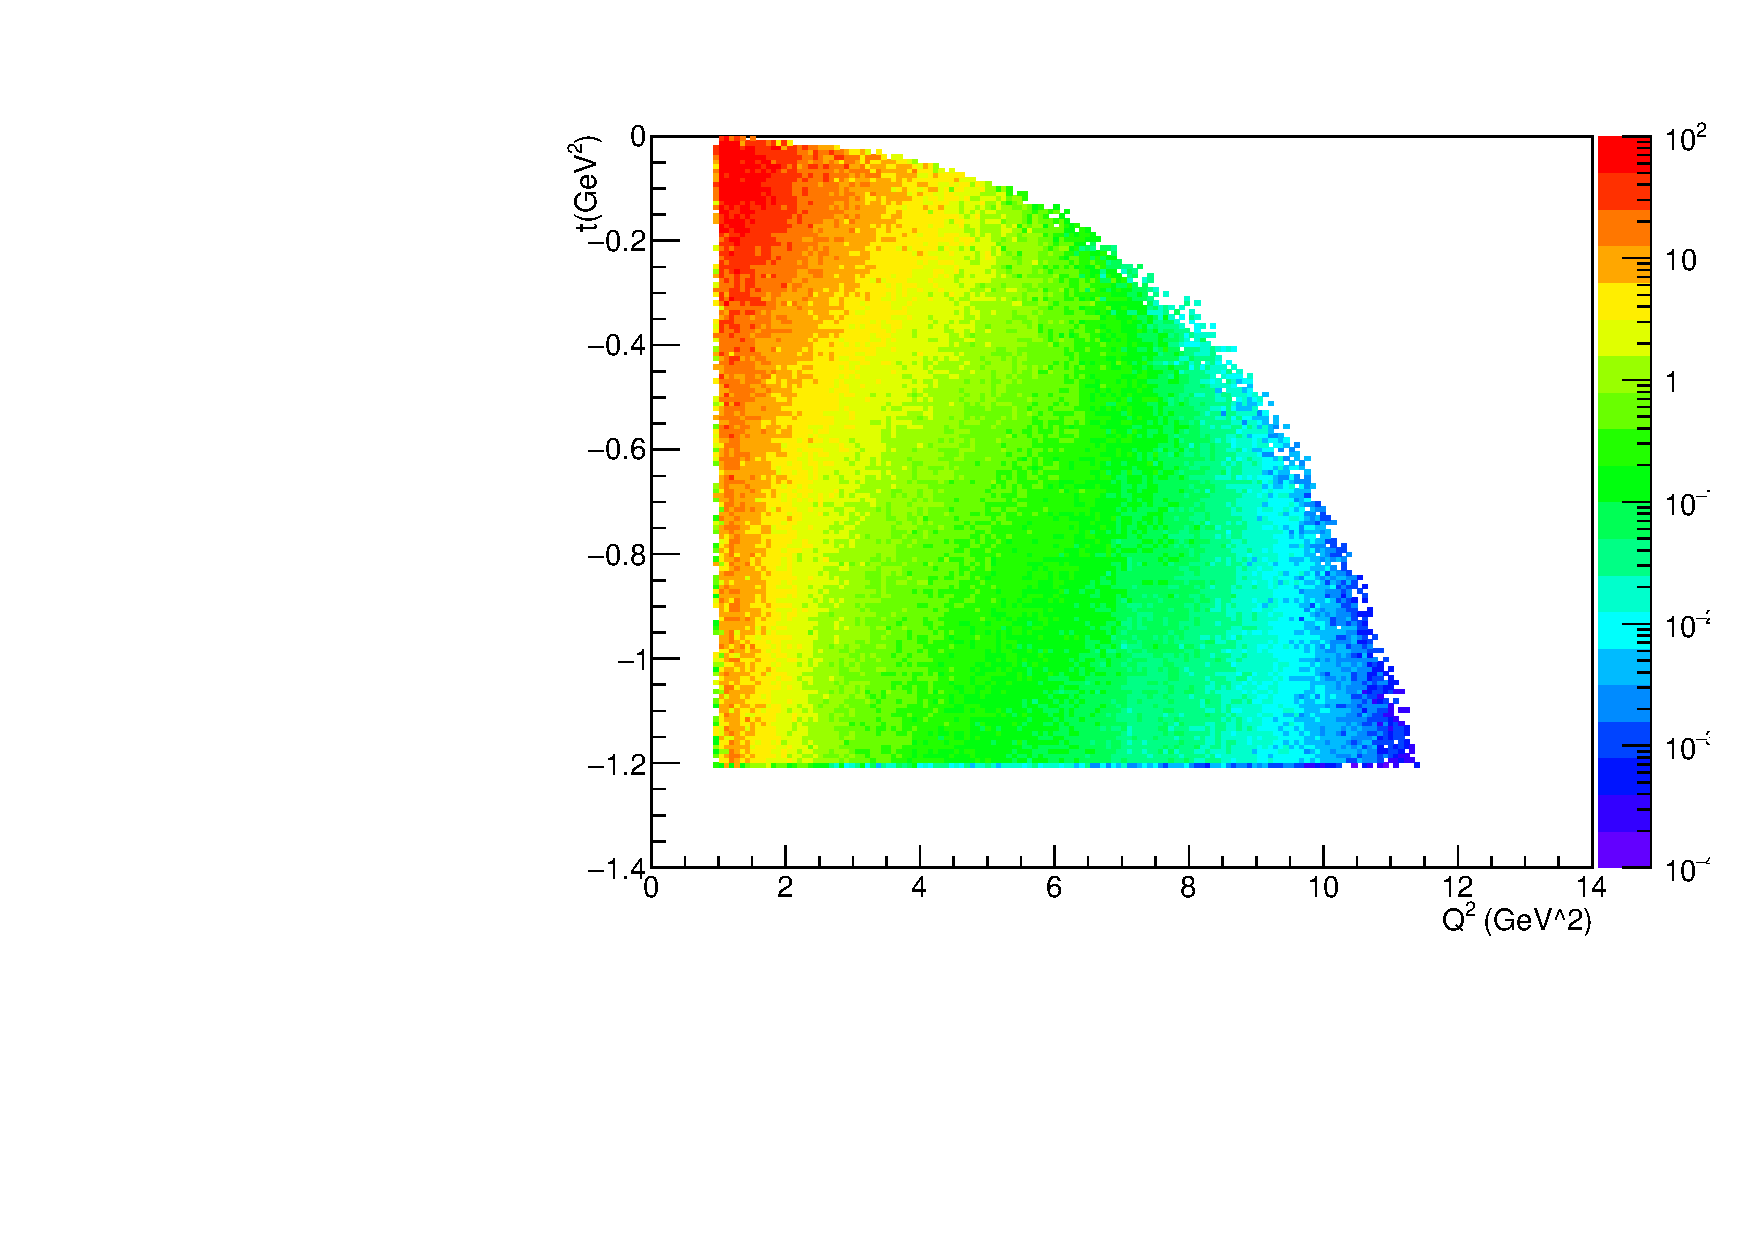
\includegraphics[width=2.9in]{tvsq2_FT.pdf}
\caption [Distributions of kinematic variables for nDVCS events]
{Distributions of kinematic variables for nDVCS events. CLAS12 acceptance cuts and physics cuts are included. Left: $Q^2$ as a function of $x_B$. Right: $t$ as a function of $Q^2$.}
\label{kine_vars}
\end{center}
\end{figure}
Kinematic cuts to ensure the applicability of the GPD formalism ($Q^2>1$ GeV$^2$/c$^2$, $t>-1.2$ GeV$^2$/c$^2$, $W>2$ GeV/c$^2$) have been applied. Figure~\ref{kine_vars} shows the coverage in $Q^2$, $x_B$ and $t$ that is obtained from the event generator for the nDVCS/BH reaction, with an electron-beam energy of 11 GeV. 

 Figures~\ref{e_th_p},~\ref{g_th_p}, and~\ref{n_th_p} show the momentum $p$ as a function of $\theta$ in the lab frame for, respectively, the electron, the photon and the neutron. As expected, the electron and the photon are mostly emitted at forward angles, while the neutron recoils at backwards angles. 

\begin{figure}[bht]
\begin{center}
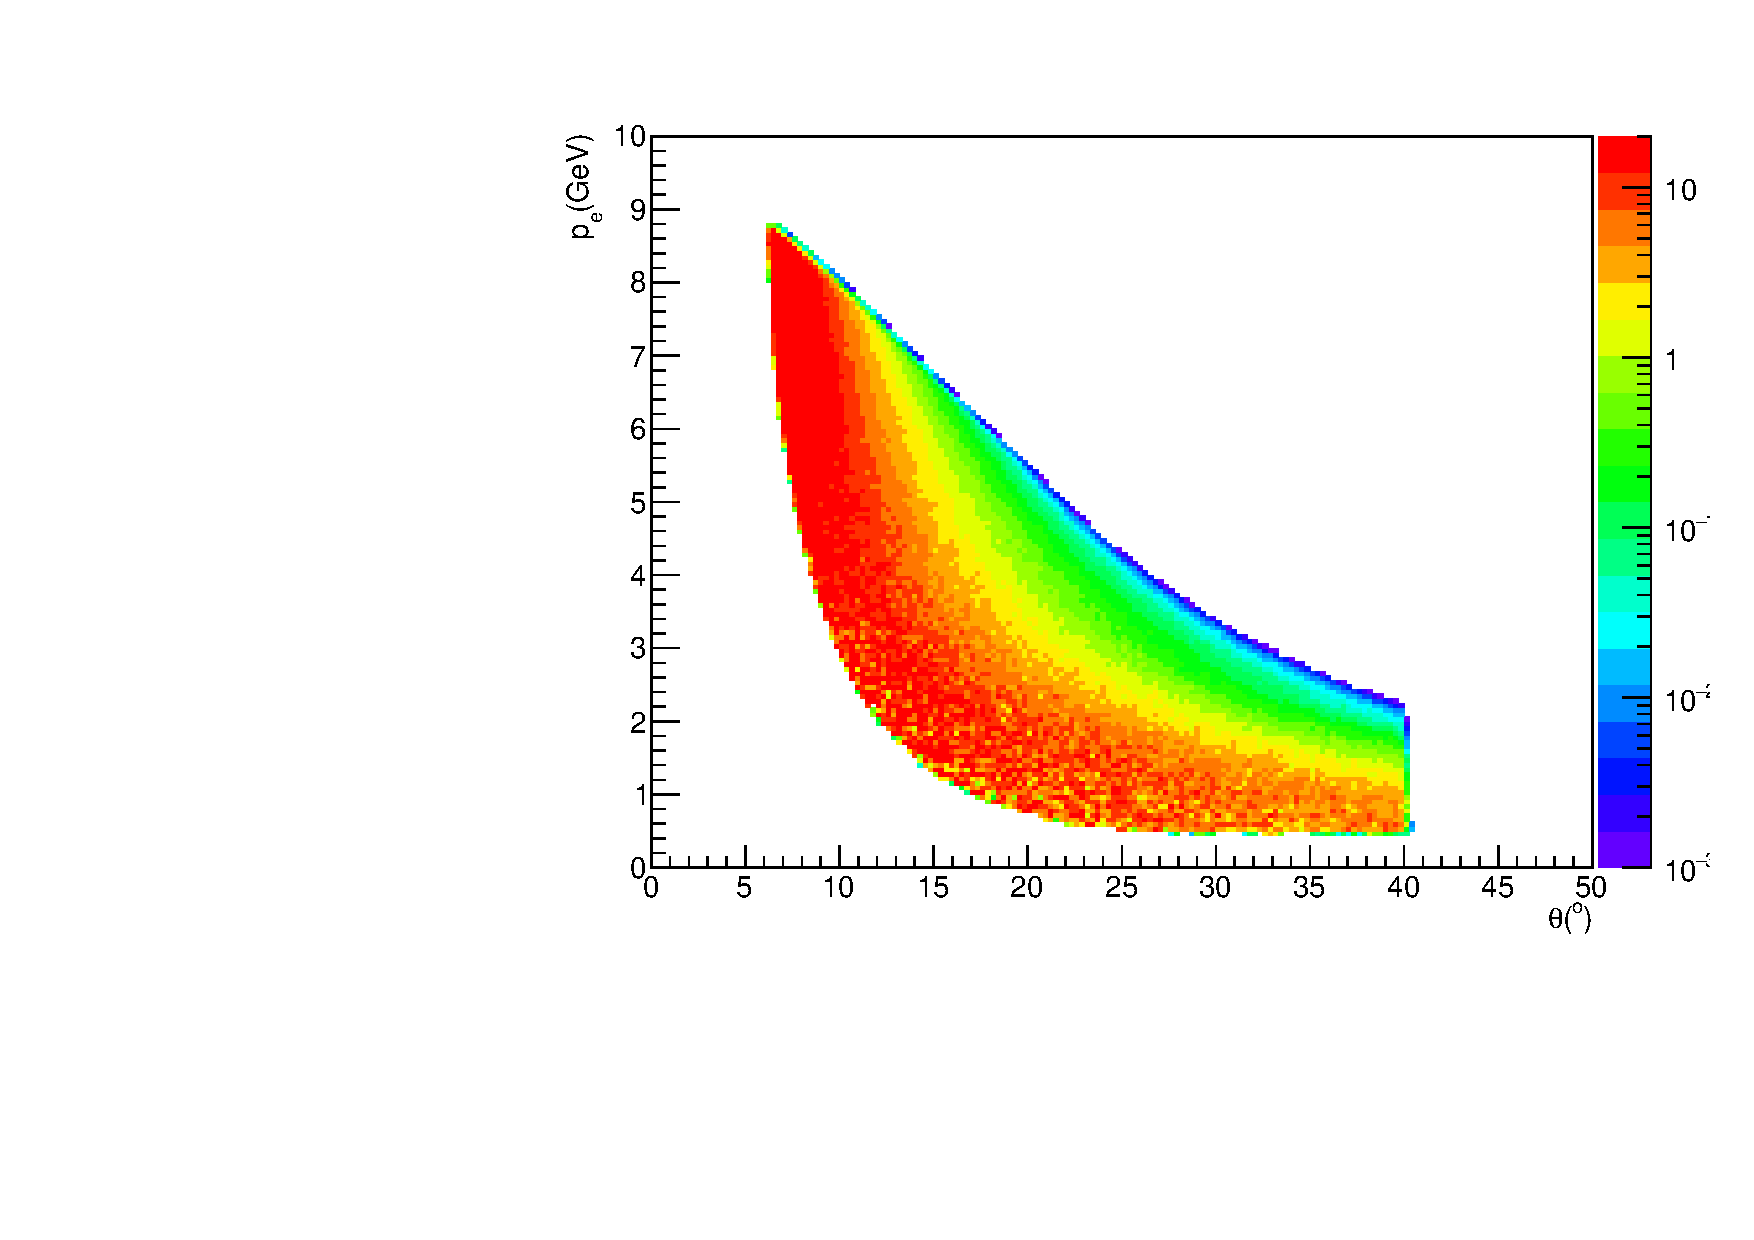
\includegraphics[width=3.2in]{theta_p_el.pdf}
\caption [Electron momentum as a function of electron polar angle]
{Electron momentum as a function of electron polar angle, for nDVCS events. CLAS12 acceptance cuts and physics cuts are included.}
\label{e_th_p}
\end{center}
\end{figure}

\begin{figure}  
\begin{center}
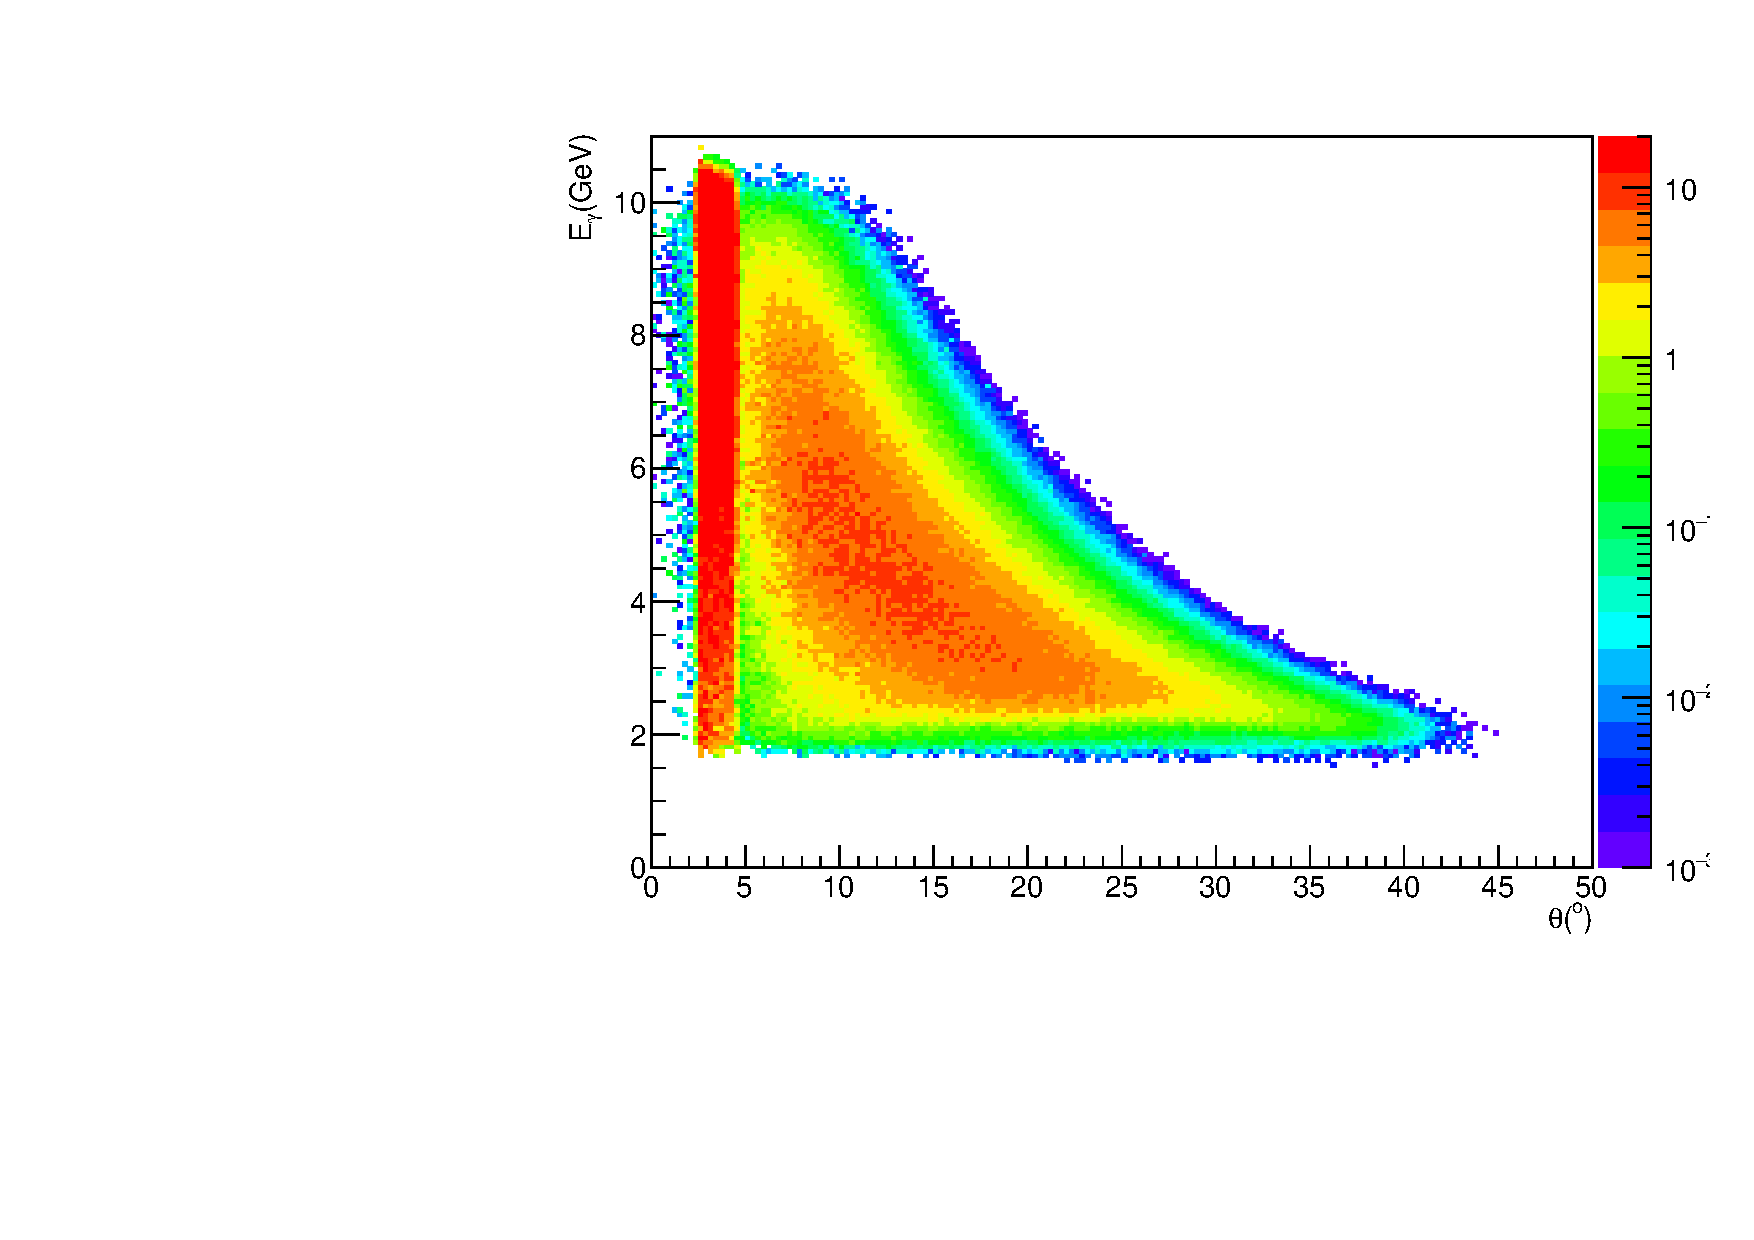
\includegraphics[width=3.2in]{theta_p_phot_FT.pdf}
\caption [Photon momentum as a function of photon polar angle, for nDVCS events]
{Photon momentum as a function of photon polar angle, for nDVCS events. CLAS12 acceptance cuts and physics cuts are included. The vertical band at low $\theta$ corresponds to photons detected in the Forward Tagger.} 
\label{g_th_p}
\end{center}
\end{figure}

\begin{figure}  
\begin{center}
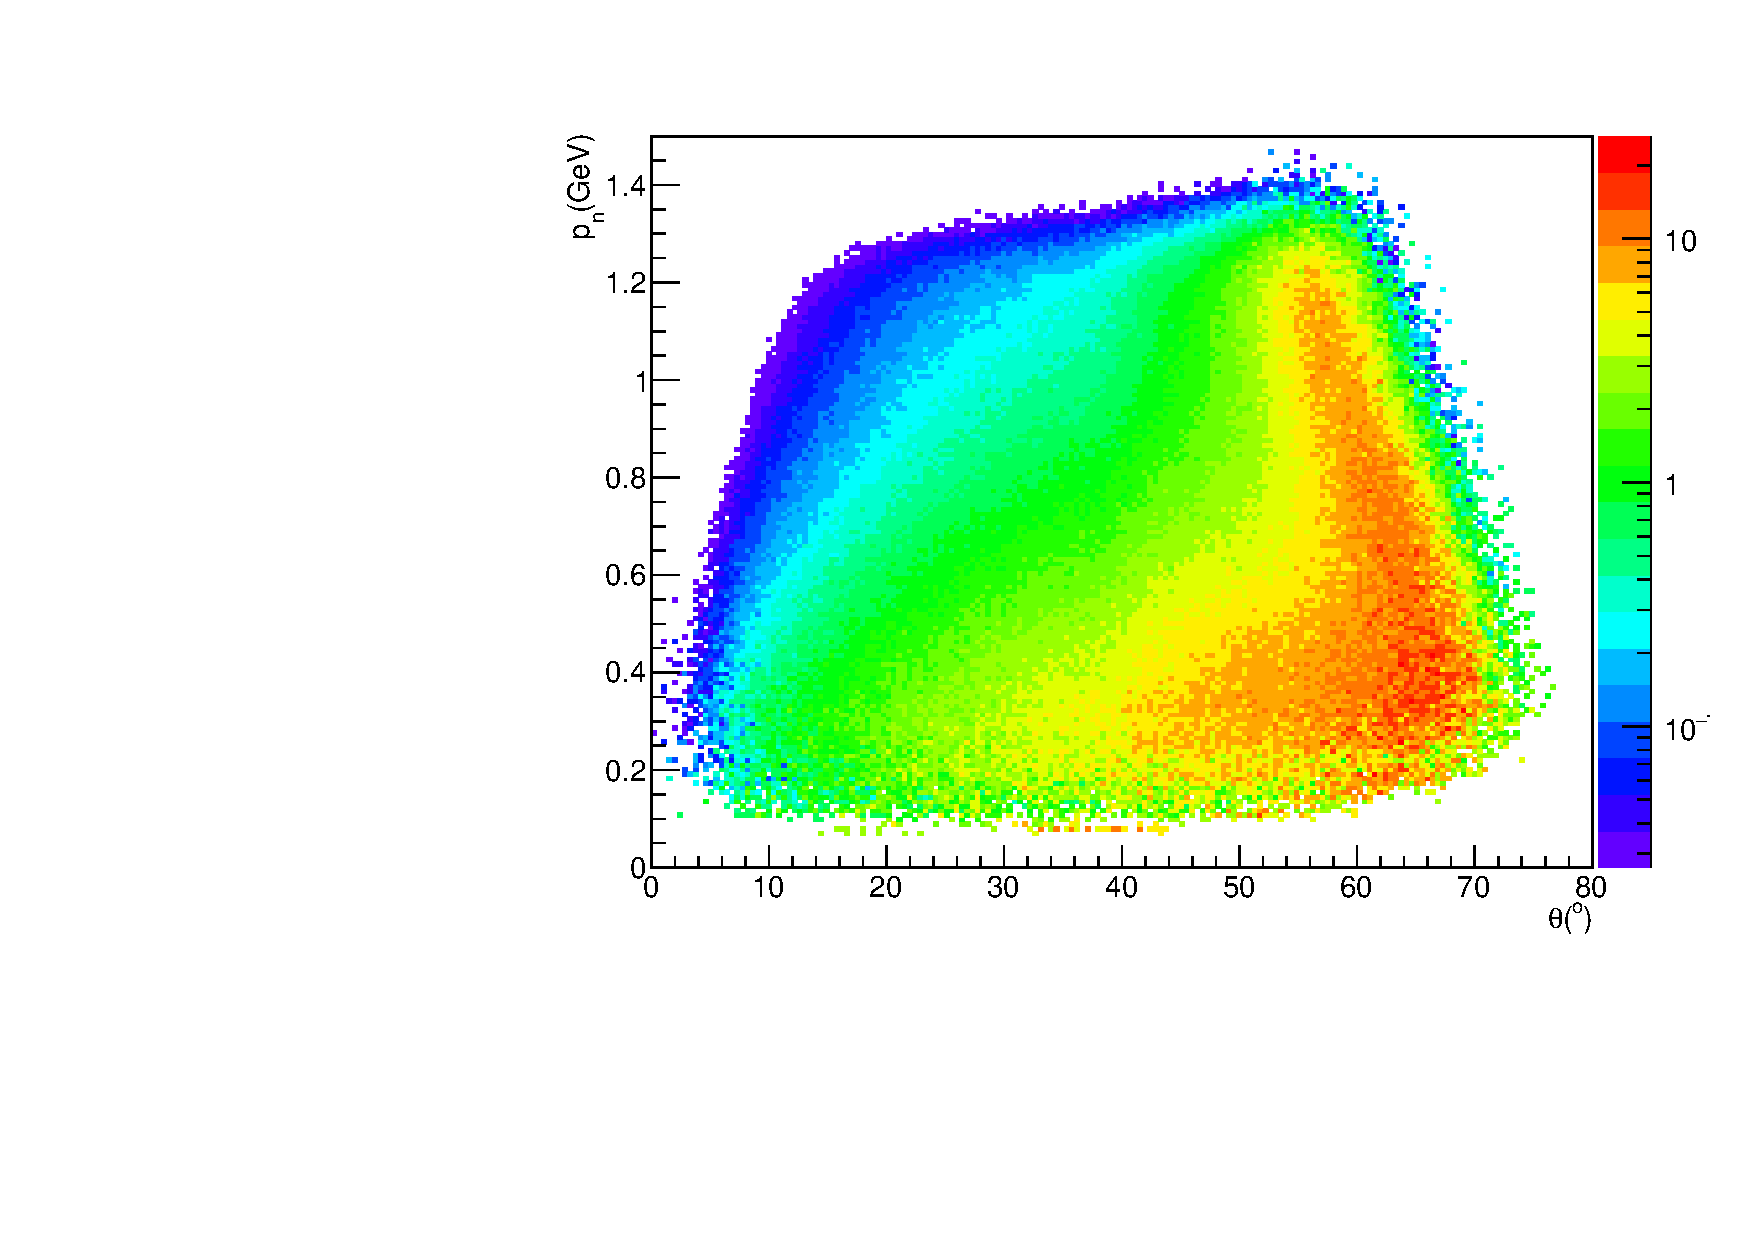
\includegraphics[width=3.2in]{theta_p_neut.pdf}
\caption [Neutron momentum as a function of neutron polar angle]
{Neutron momentum as a function of neutron polar angle, for nDVCS events. CLAS12 acceptance cuts and physics cuts are included.}
\label{n_th_p}
\end{center}
\end{figure}

\section{Measurement of the asymmetries}
We plan to extract two kinds of asymmetries, the experimental definitions of which are given here. In all of the formulae below, the first sign in the superscript on the number of normalized DVCS/BH events $N$ is the beam helicity ($b$) and the second sign
is the target polarization ($t$).
$N$ is obtained from $en\gamma$ events ($N_{en\gamma}$), normalized by the corresponding Faraday-cup charge ($FC^{bt}$) after subtraction of the $\pi^0$ background as follows:
\begin{equation}
N^{bt}= (1-B_{\pi^0}^{bt})\cdot \frac{N^{bt}_{en\gamma}}{FC^{bt}},
\end{equation}

where $B_{\pi^0}$ is the relative $\pi^0$ contamination, outlined in Section \ref{sec_pi0_back}. 

The target-spin asymmetry will be computed as:
\begin{equation}\label{def_tsa}
A_{\rm UL} = \frac{N^{++}+N^{-+}-N^{+-}-N^{--}}{D_f (P_t^-(N^{++}+N^{-+})+P_t^+(N^{+-}+N^{--}))}~.
\end{equation}
 $D_f$ is the dilution factor to account for the contribution of the unpolarized background (Section \ref{sec_dilution}), and $P_t$ is the polarization of the target. 

The double (beam-target) spin asymmetry will be obtained as:

\begin{equation}\label{def_dsa}
A_{\rm LL} = \frac{N^{++}+N^{--}-N^{+-}-N^{-+}}{P_b\cdot D_f (P_t^-(N^{++}+N^{-+})+P_t^+(N^{+-}+N^{--}))}
\end{equation}
where $P_b$ is the polarization of the beam.

In the following, the steps leading to the extraction from the data of all the terms composing these asymmetries will be presented. 

\subsection{Event selection and exclusivity cuts}\label{sec_excl_cuts}
After selecting events with exactly one electron (in the forward part of CLAS12) and one neutron (in the CND and in the EC), and at least one photon (in the EC or in the FT), and applying the appropriate PID and fiducial cuts, further cuts need to be applied to ensure the exclusivity of the DVCS/Bethe-Heitler final state. Two kinds of backgrounds need, in fact, to be removed, or reduced as much as possible: the nuclear background coming from scattering on the nitrogen of the ND$_3$ target, and the background coming from other channels containing electron, neutron and at least one photon in the final state. Having measured the four-vectors of the three active final-state particles, one can construct several observables (hereafter referred to as ``exclusivity variables'') on which cuts can be applied to select the DVCS/BH channel. Here, the following quantities were studied, with the aid of our nDVCS and $en\pi^0(p)$ simulations:
\begin{itemize}
\item{the squared missing mass of $X$, in the $ed\to en\gamma X$ reaction;}
\item{the momentum of the spectator proton, obtained as $p(X)$ from $ed\to en\gamma X$;}
\item{the squared missing mass of $X$, in the $en\to en\gamma X$ reaction, assuming the initial neutron to be at rest;}
\item{the missing energy of $X$, in the $ed\to en\gamma X$ reaction;}
\item{$p_{perp}$, the transverse component of the missing momentum of the reaction $en\to en\gamma X$, given by $p_{perp}=\sqrt{p_x(X)^2+p_y(X)^2}$.}
\end{itemize}

Figures~\ref{dvcs_excl} and \ref{pi0_excl} show the exclusivity variables listed above for, respectively, nDVCS simulated events and $en\pi^0(p)$ simulated events for which only one electron, one neutron and one photon of energy above 2 GeV fell within the CLAS12 acceptance. The red lines represent the exclusivity cuts, the values of which were choosen to maximize the number of nDVCS events retained while reducing the $en\pi^0(p)$ background as much as possible. It must be stressed that the event generator adopted here does not contain Fermi motion effects coming from the nitrogen of the ND$_3$ target. The experimental distributions of the exclusivity variables will therefore be broader, and the peaks will be masked by the nuclear background. 
However, it was shown in the eg1-DVCS analysis \cite{pisano} that peaks due to the pDVCS channel became evident when appropriately rescaled spectra from a $^{12}$C background target were subtracted from the exclusivity variable distributions.  We plan to adopt a similar approach here.

\begin{figure}
\begin{center}
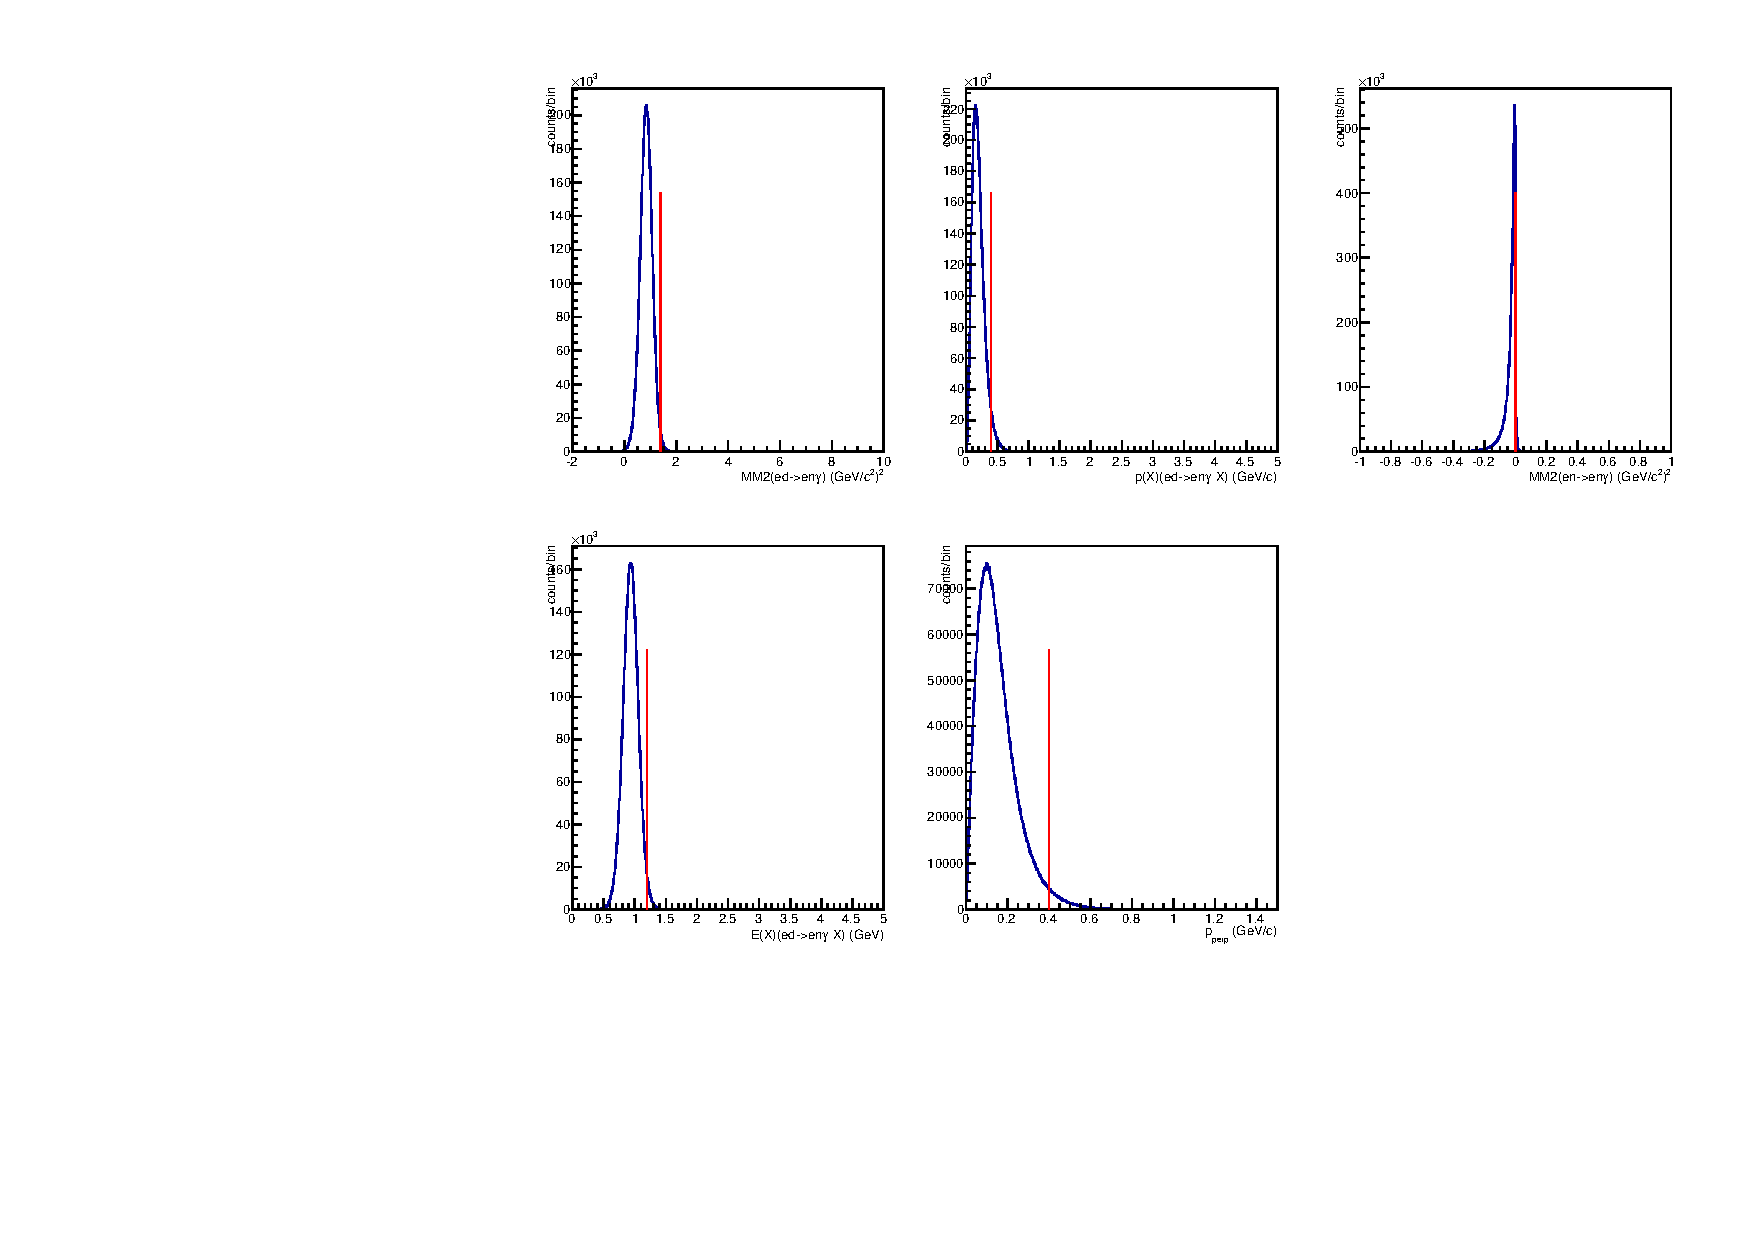
\includegraphics[width=120mm]{dvcs_excl_vars_noFT_100days.pdf}
\caption[nDVCS simulation, after FastMC]
{nDVCS simulation, after FastMC: DVCS exclusivity variables. Starting from the top left: MM$^2_X(ed\to en\gamma X)$, $p(X)(ed\to en\gamma X)$,  MM$^2_X(en\to en\gamma X)$, $E(X)(ed\to en\gamma X)$, $p_{perp}$. The red lines mark the values adopted for the nDVCS exclusivity cuts.}
\label{dvcs_excl}
\end{center}
\end{figure}

\begin{figure}
\begin{center}
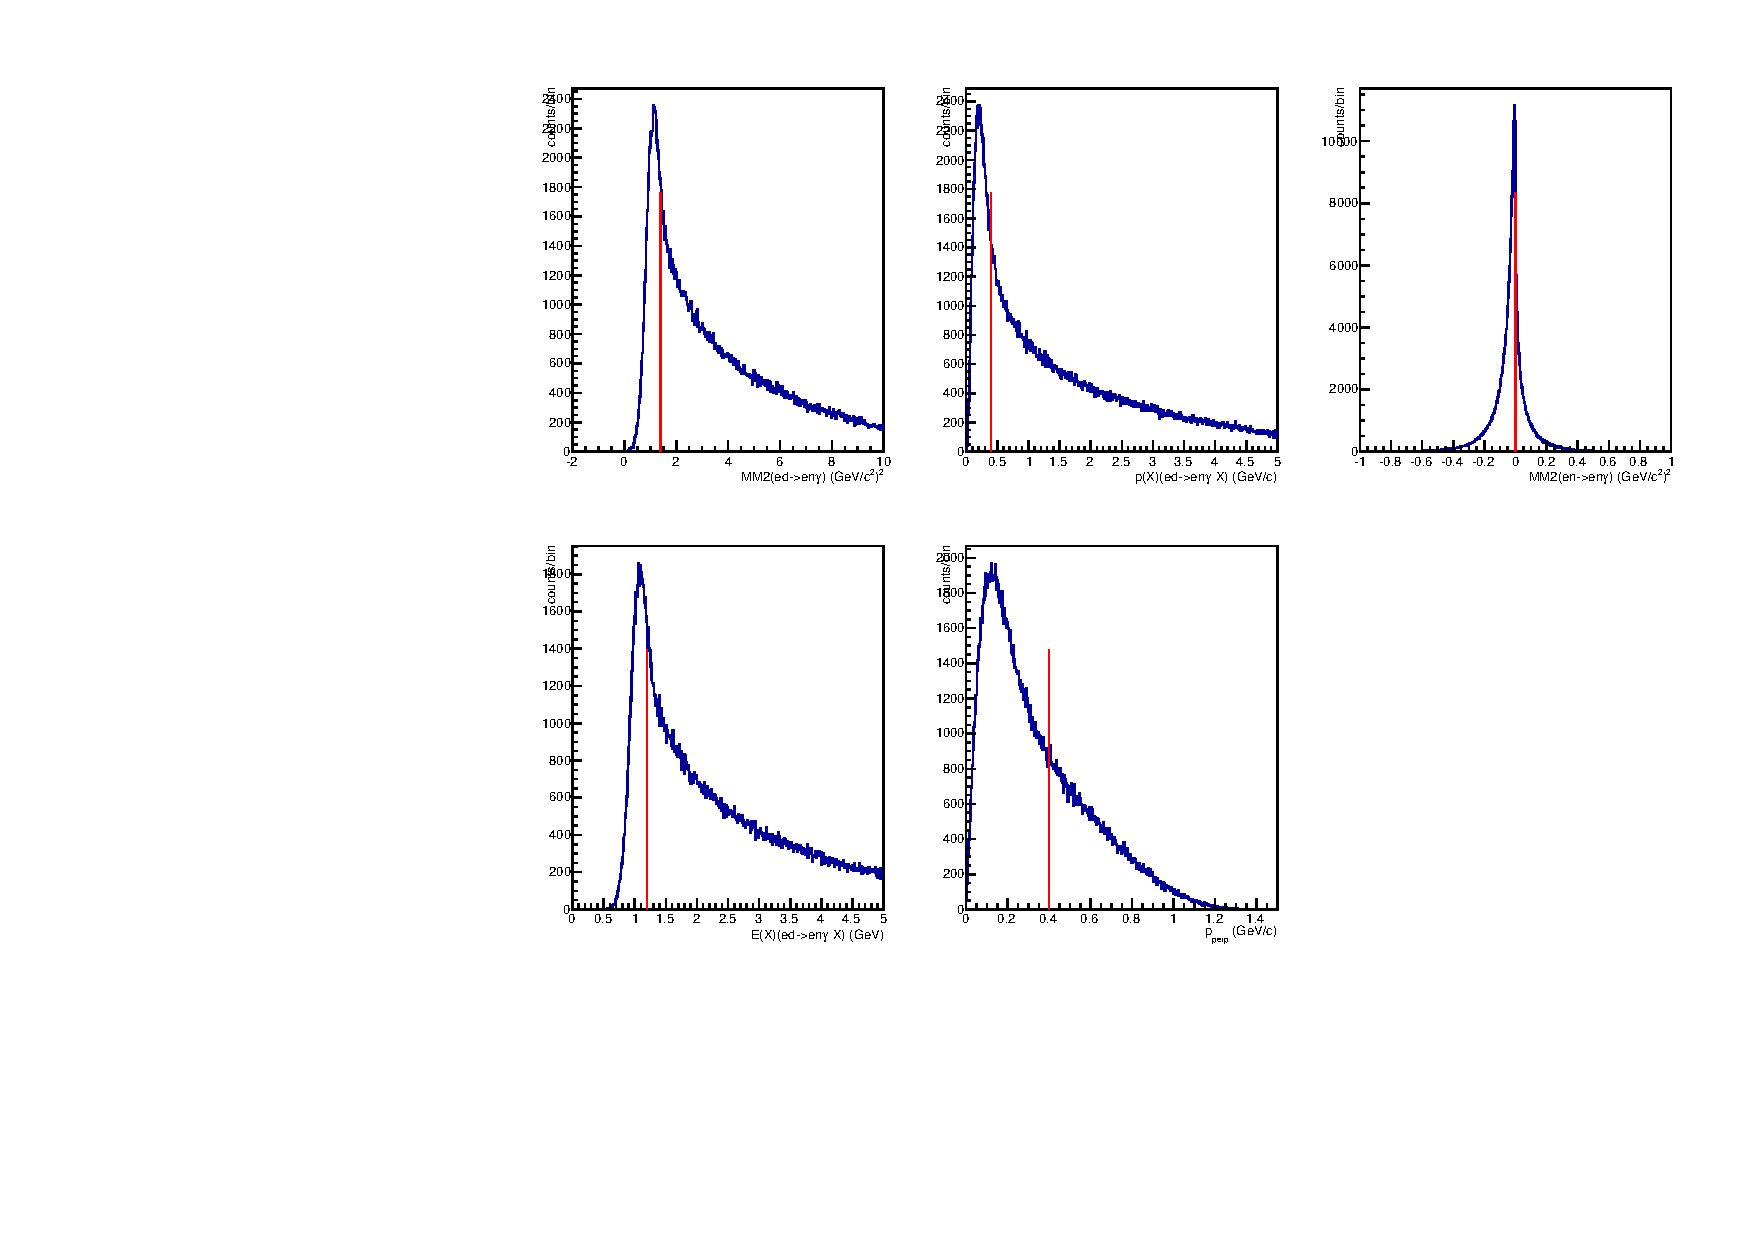
\includegraphics[width=120mm]{pi0_excl_vars_noFT_100days.pdf}
\caption[$\pi^0$ simulation, after FastMC]
{$\pi^0$ simulation, after FastMC, events for which only one electron, one neutron and one photon of energy above 2 GeV fell within the CLAS12 acceptance: DVCS exclusivity variables, same as Fig.~\ref{dvcs_excl}. The red lines mark the values adopted for the nDVCS exclusivity cuts.}
\label{pi0_excl}
\end{center}
\end{figure}

The expected $en\pi^0(p)$ contamination that remains after these cuts is shown in Fig.~\ref{ndvcs-pi0}, where the ratio of surviving $en\pi^0(p)$ events to the number of nDVCS events is plotted as a function of $\phi$, integrated over the other kinematic variables. It ranges from 0, at the extreme $\phi$ values, to about $40\%$, in the central $\phi$ range. This background can be evaluated and subtracted from the final asimmetries, as will be described in Section~\ref{sec_pi0_back}. 

\begin{figure}  
\begin{center}
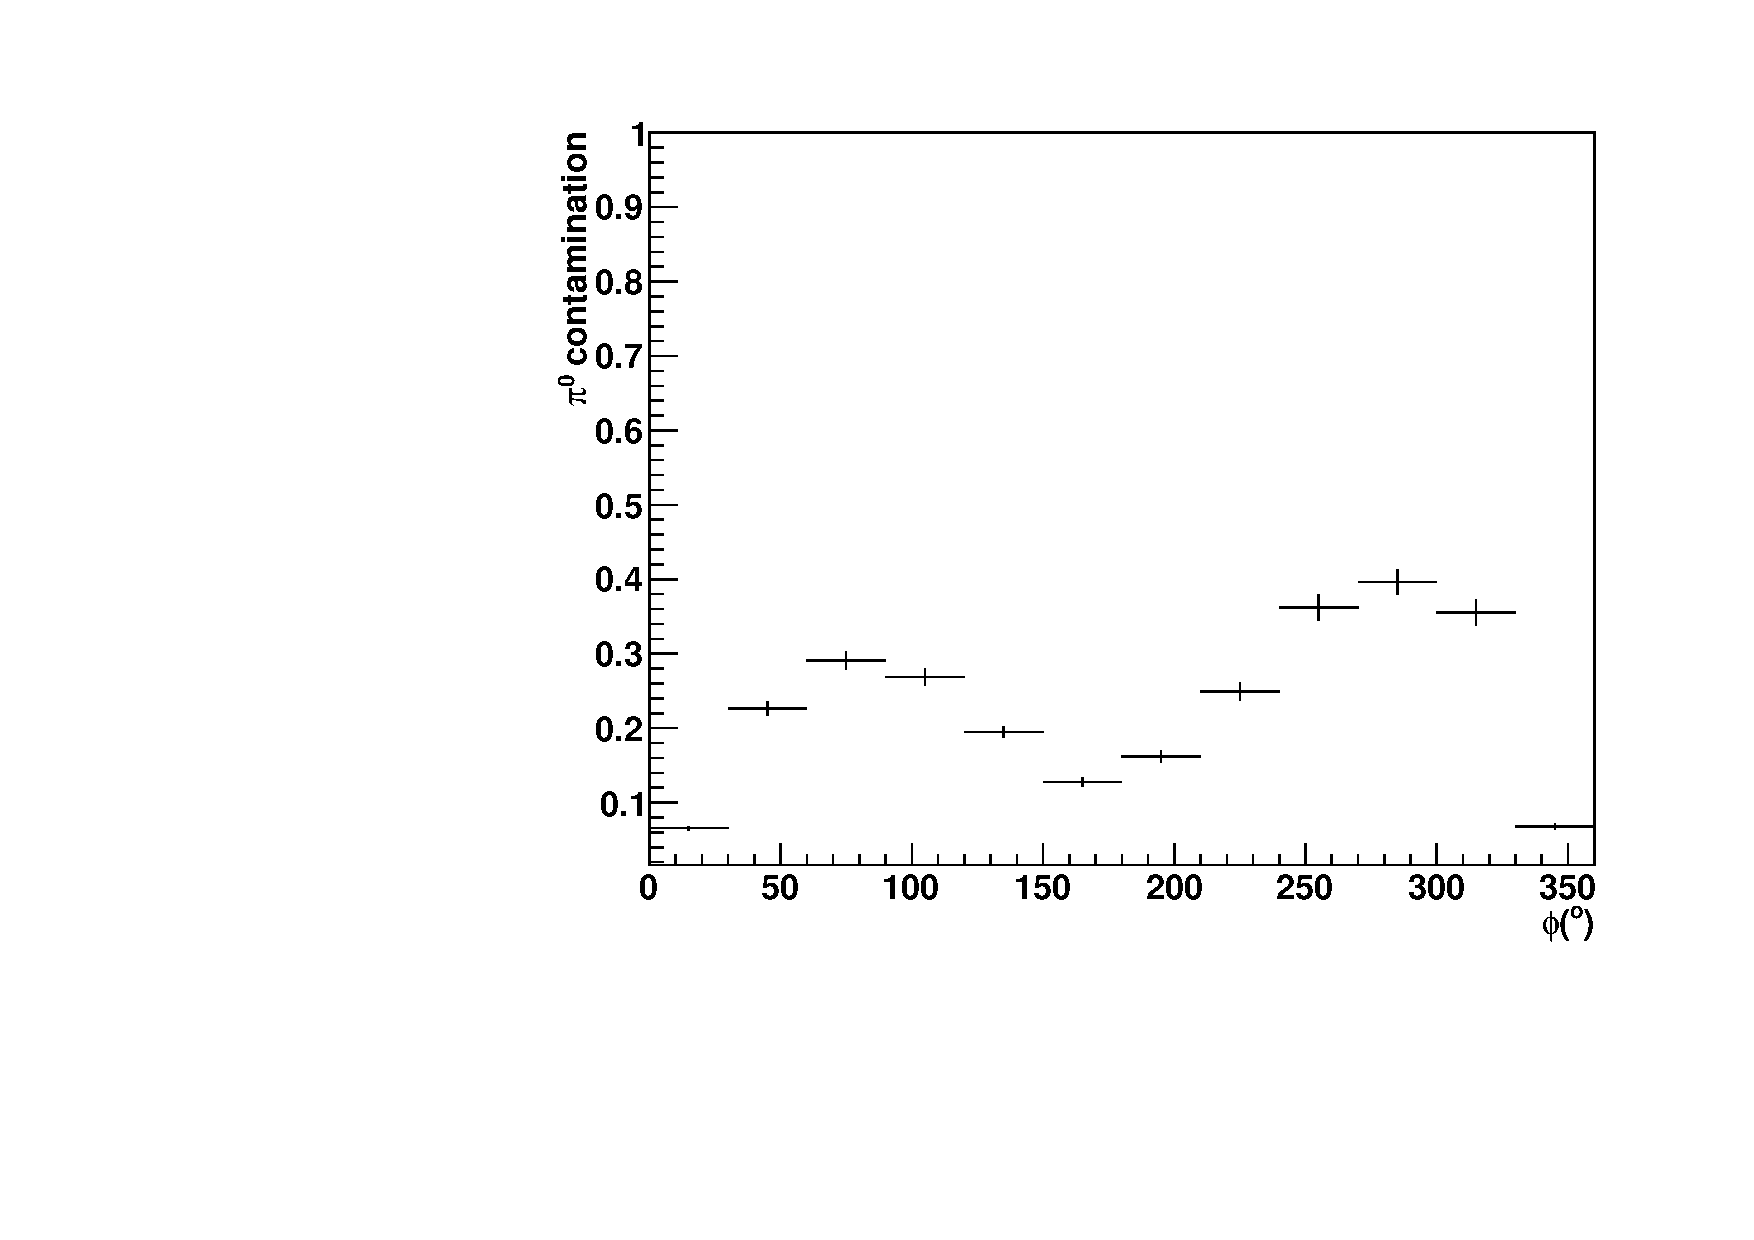
\includegraphics[width=80mm]{pi0_integrated_100days_noFT.pdf}
\caption [Expected $\pi^0$ contamination fraction as a function of $\phi$]
{Expected $\pi^0$ contamination fraction for the proposed experiment, defined as $\frac{N_{\pi^{0} 1\gamma}}{N_{en\gamma}}$, as a function of $\phi$ and integrated over the other kinematic variables. }
\label{ndvcs-pi0}
\end{center}
\end{figure}

An exploratory nDVCS analysis on the ND$_3$ subset (``part C'') of the CLAS
eg1-dvcs data-set is underway \cite{daria_eg1dvcs}. In spite of the very poor
statistics and the far from optimal neutron reconstruction in the CLAS
EC calorimeters, a selection of the nDVCS final state has been possible.
Figure~\ref{ndvcs_daria} shows the same exclusivity variables as are plotted in
Fig.~\ref{dvcs_excl}, obtained after applying nDVCS selection cuts to the $en\gamma$ event sample, which were optimised for the eg1-dvcs data. The similarities with our simulations are remarkable, especially considering that no nuclear background was subtracted from the distributions of Fig.~\ref{ndvcs_daria}, which gives confidence in this data-selection technique for the proposed experiment. Additionally, the effect of nuclear background subtraction can be seen in Fig.~\ref{daria_sub}, which shows the missing mass squared from $en\to enX$ before and after subtraction of opportunely scaled distributions obtained with carbon data,
and in Fig.~\ref{daria_sub_fit} , displaying the carbon-subtracted $m_{X}^{2}$ 
distribution from $en \to en\gamma X$. The figure indicates that a good selection of the $en\gamma$ final state has been possible even within the limitations 
of the eg1-dvcs experiment and illustrate the applicability of the 
technique to the proposed experiment.

\begin{figure}
\begin{center}
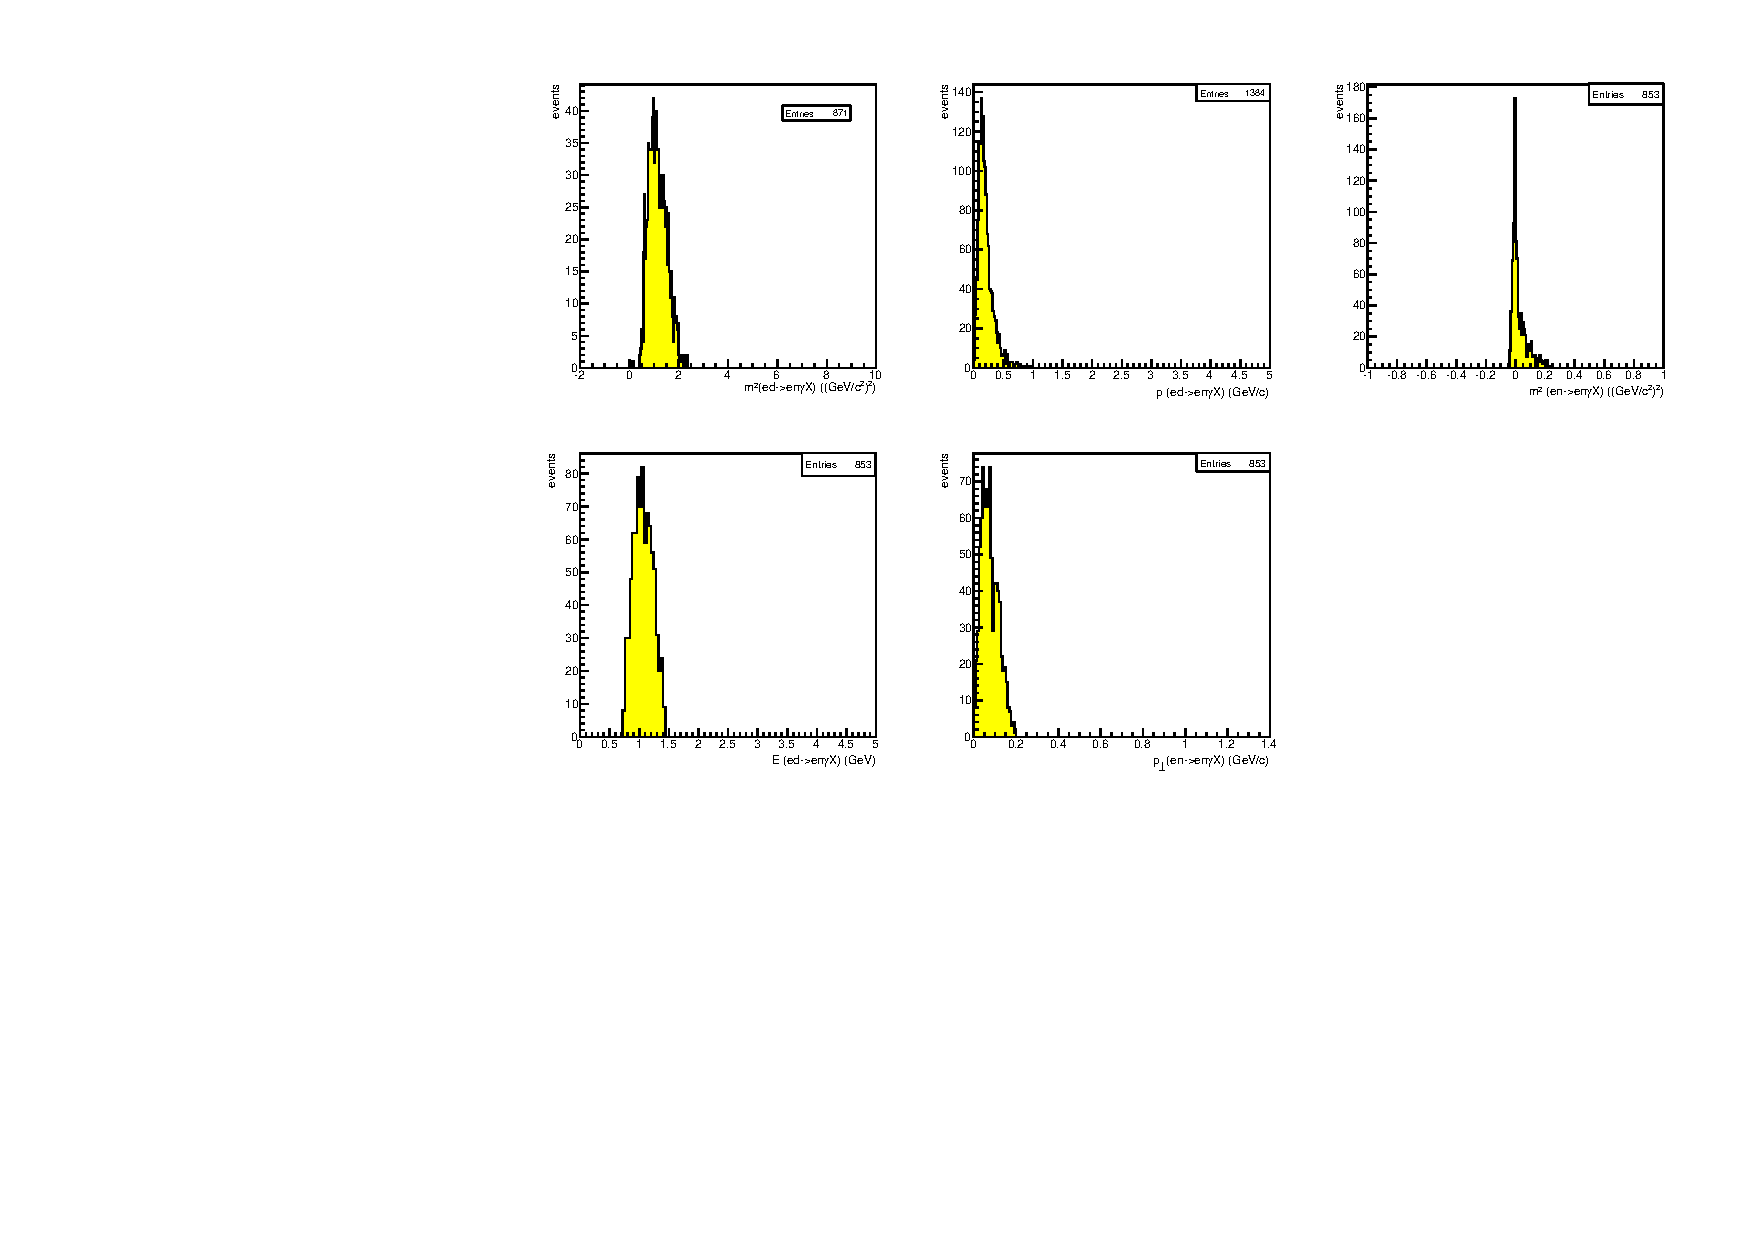
\includegraphics[width=120mm]{nDVCS_data_exclusivity.pdf}
\caption[nDVCS, CLAS eg1-dvcs analysis]
{nDVCS analysis of the CLAS eg1-dvcs data set, after exclusivity cuts: DVCS exclusivity variables, same as Fig.\ref{dvcs_excl}.}
\label{ndvcs_daria}
\end{center}
\end{figure}

\begin{figure}
\begin{center}
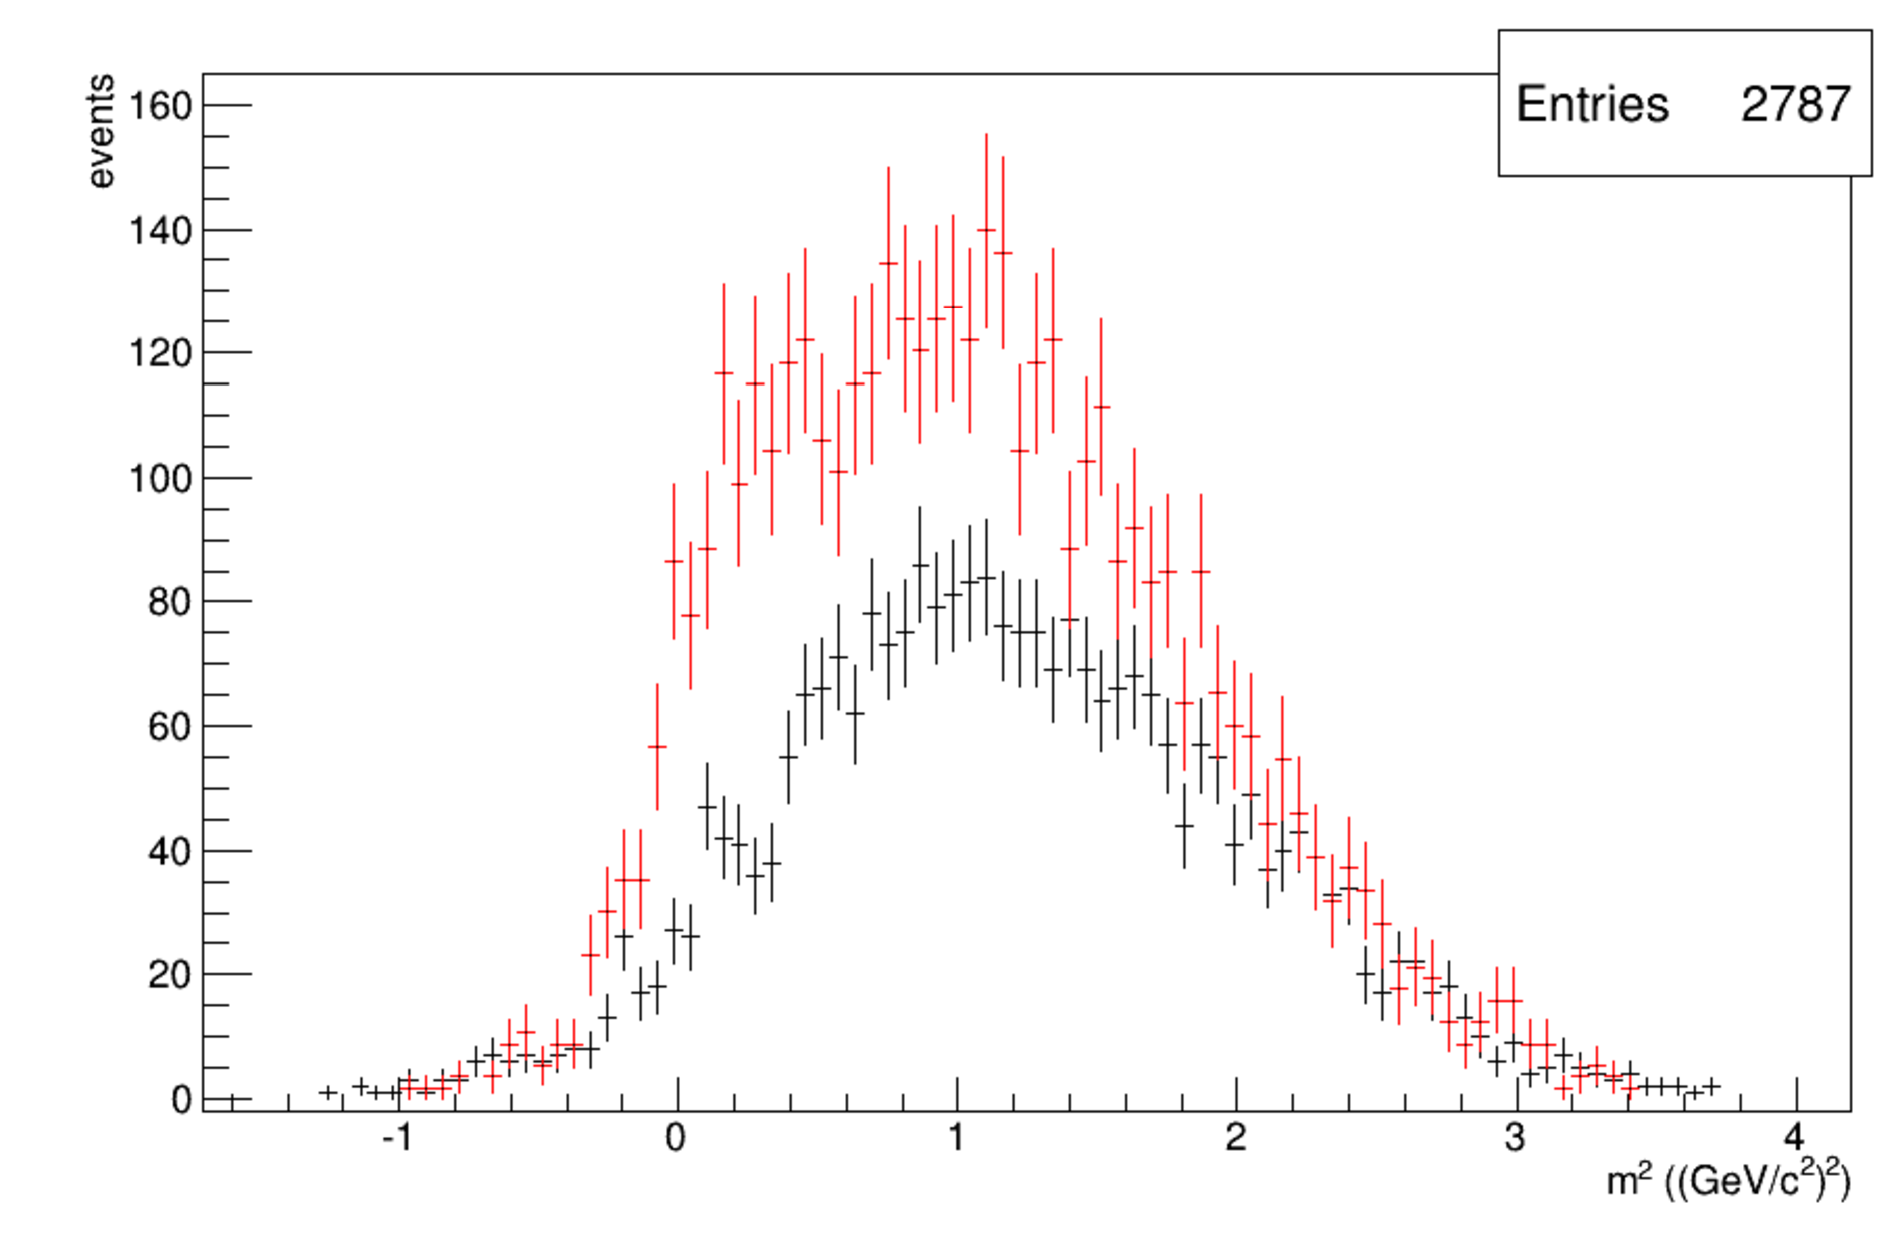
\includegraphics[width=80mm]{mm2_en.pdf}
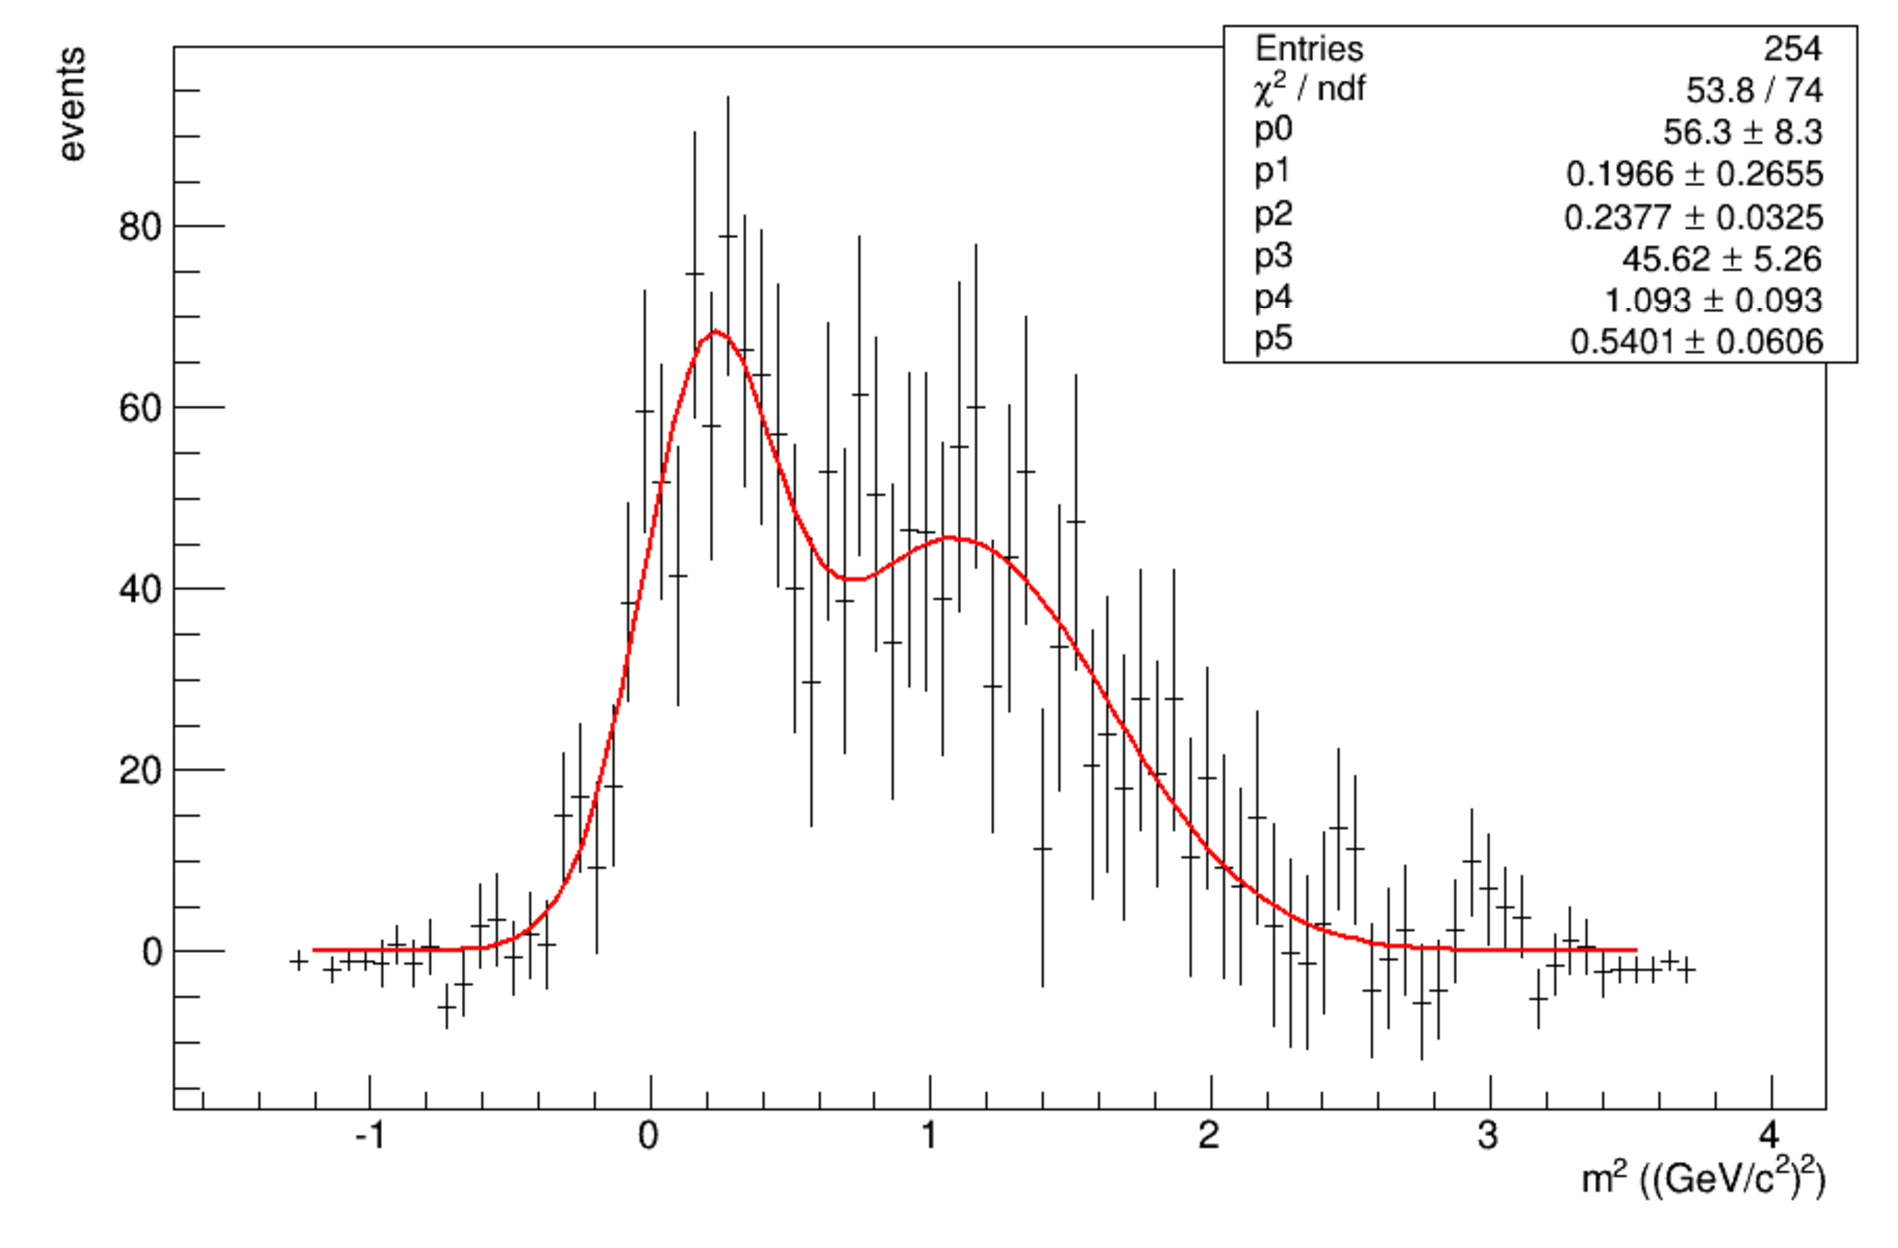
\includegraphics[width=80mm]{mm2_en_fit.pdf}
\caption 
{nDVCS analysis of the CLAS eg1-dvcs data set. Top: squared missing mass of $X$ in $en\to enX$, with ND$_{3}$ (red) and carbon (black); bottom: after carbon subtraction, a peak near 0 appears. }   
\label{daria_sub}
\end{center}
\end{figure}

\begin{figure}
\begin{center}
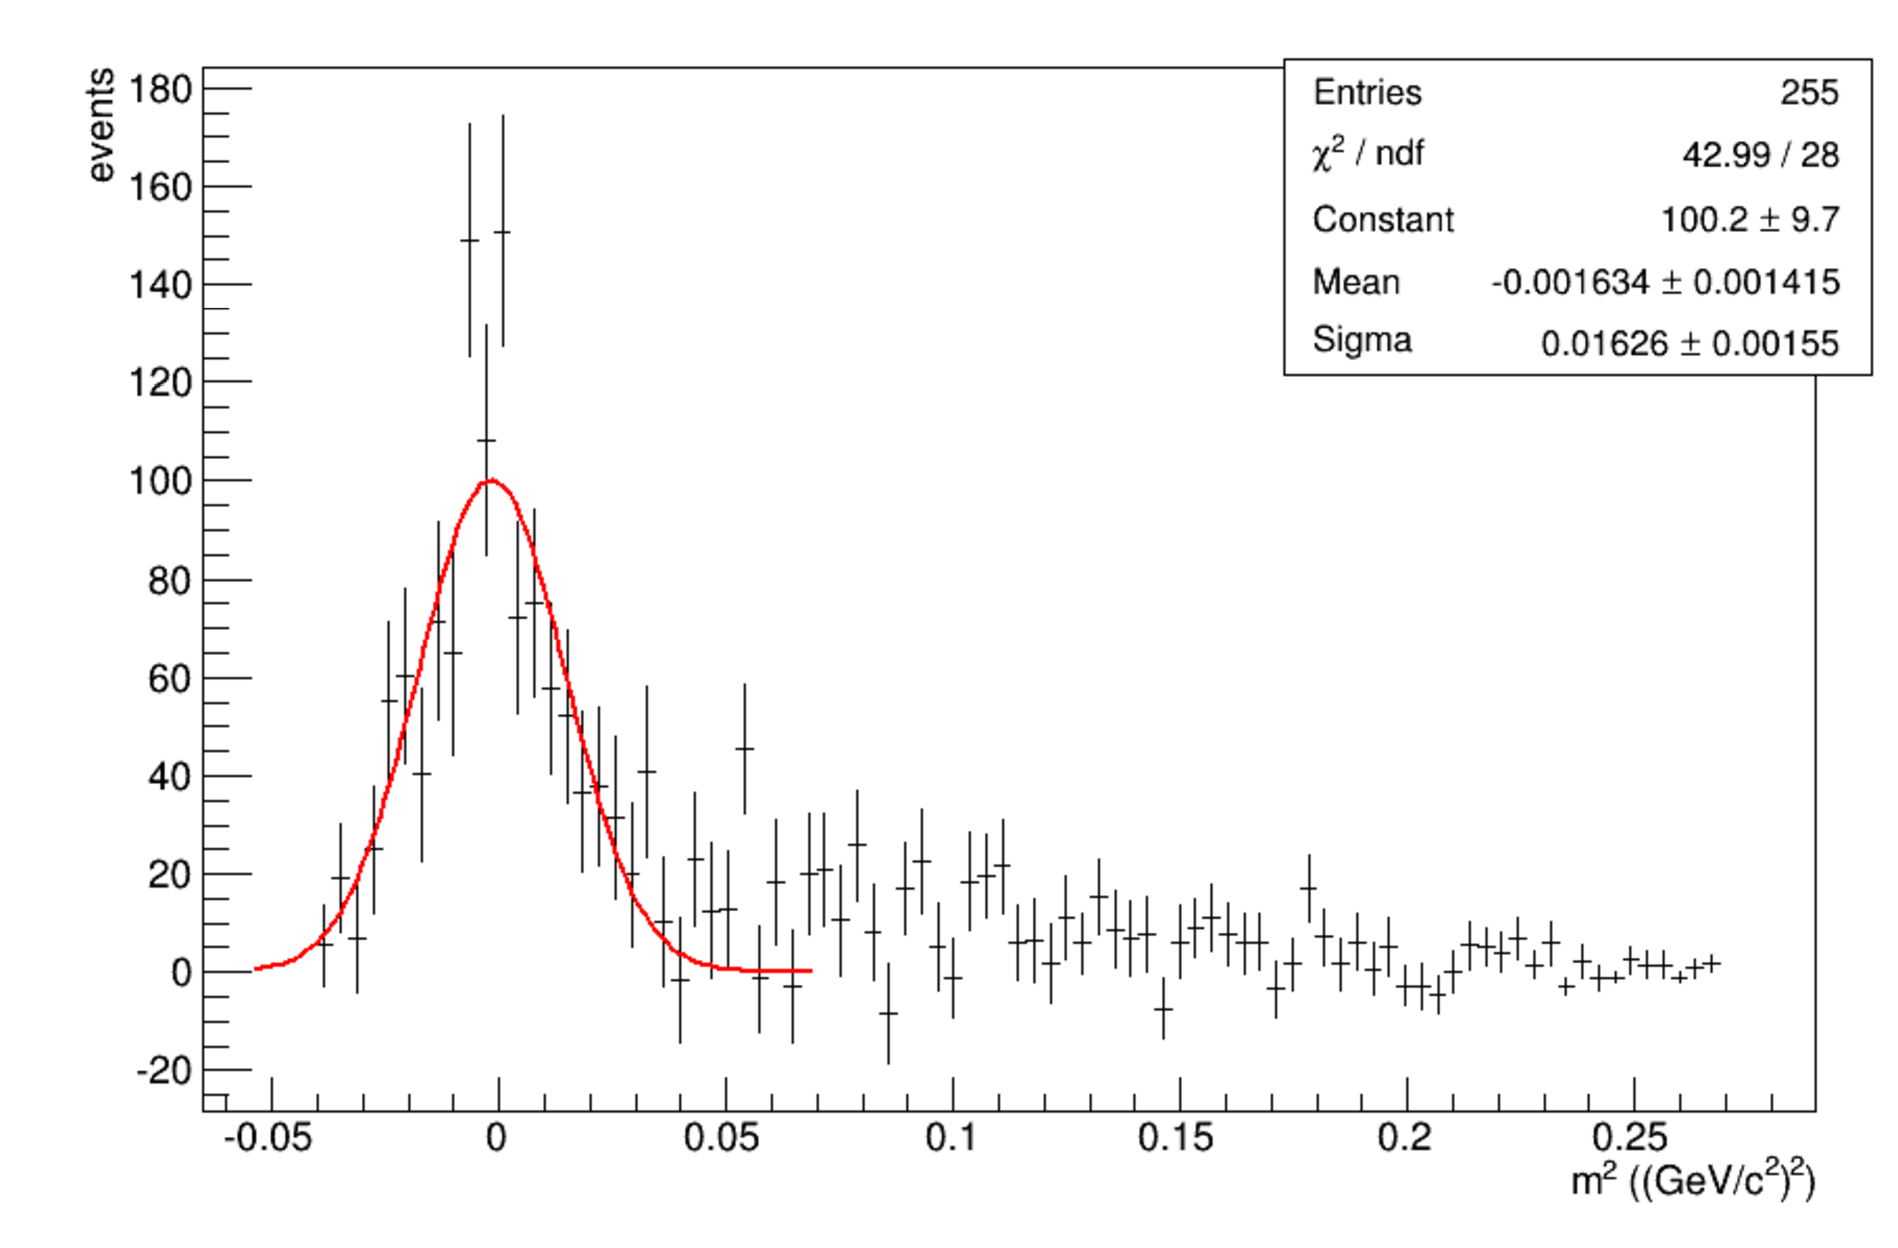
\includegraphics[width=80mm]{mm2_eng_fit.pdf}
\caption
{nDVCS analysis of the CLAS eg1-dvcs data set: squared missing mass of $X$ in $en\to en\gamma X$, after exclusivity cuts and carbon subtraction.}
\label{daria_sub_fit}
\end{center}
\end{figure}

\section{Neutral pion background }\label{sec_pi0_back}

Once the events containing one electron, one active neutron and one energetic photon are selected, and no other charged particles are detected in CLAS12, the nDVCS/BH final state can be isolated by cutting on the $en\gamma$ missing mass and the other exclusivity variables. These selection criteria will eliminate the majority of the competing channels, such as, for instance, charge-exchange reactions on the proton, where a positively charged meson (mostly a $\pi^+$) is emitted along with the neutron. 
However, due to the finite resolutions of the detectors, the final event sample will still be contaminated by $en\gamma$ events coming from the $en\pi^0(p)$ channel, where one photon from the $\pi^0$ decay is detected in the forward part of CLAS12 while the other escapes detection. This contamination will be evaluated and subtracted as was done in previous DVCS CLAS analyses \cite{fx,erin,pisano,hs}, by extracting exclusive $en\pi^0(p)$ events --- detecting both decay photons --- from the data, and using Monte Carlo simulations to evaluate the ratio of acceptances of $\pi^0$ events with 1 and 2 photons detected. The final number of nDVCS/BH events, in each 4-dimensional bin, will be obtained as:

\begin{eqnarray}
N_{DVCS}(Q^2,x_B,-t,\phi)=N_{en\gamma}(Q^2,x_B,-t,\phi)-N_{\pi^0 1\gamma}(Q^2,x_B,-t,\phi)
\end{eqnarray}
where
\begin{eqnarray}\label{pi0_formula}
N_{\pi^0 1\gamma}(Q^2,x_B,-t,\phi)=N^{data}_{\pi^0}(Q^2,x_B,-t,\phi)\cdot \frac{N^{MC}_{\pi^0 1\gamma}(Q^2,x_B,-t,\phi)}{N^{MC}_{\pi^0 2\gamma}(Q^2,x_B,-t,\phi)}
\end{eqnarray}

As an example, Fig.~\ref{pi0_eg1dvcs} shows the elements contributing to the $\pi^0$ background subtraction, as were evaluated for the extraction of the TSA in the CLAS eg1-dvcs analysis, for two particular kinematic bins in $(Q^2, x_B, -t)$. Note that the impact on the final asymmetry of the background subtraction is quite small: an average effect of roughly 10\%, relative to the value of the TSA at $90^{\circ}$, was estimated for this data set. In fact, what will impact the final asymmetries is not the size of the contamination itself, but the point-by-point difference of contamination for positive and negative target (or beam-target) polarization. 

\begin{figure}  
\begin{center}
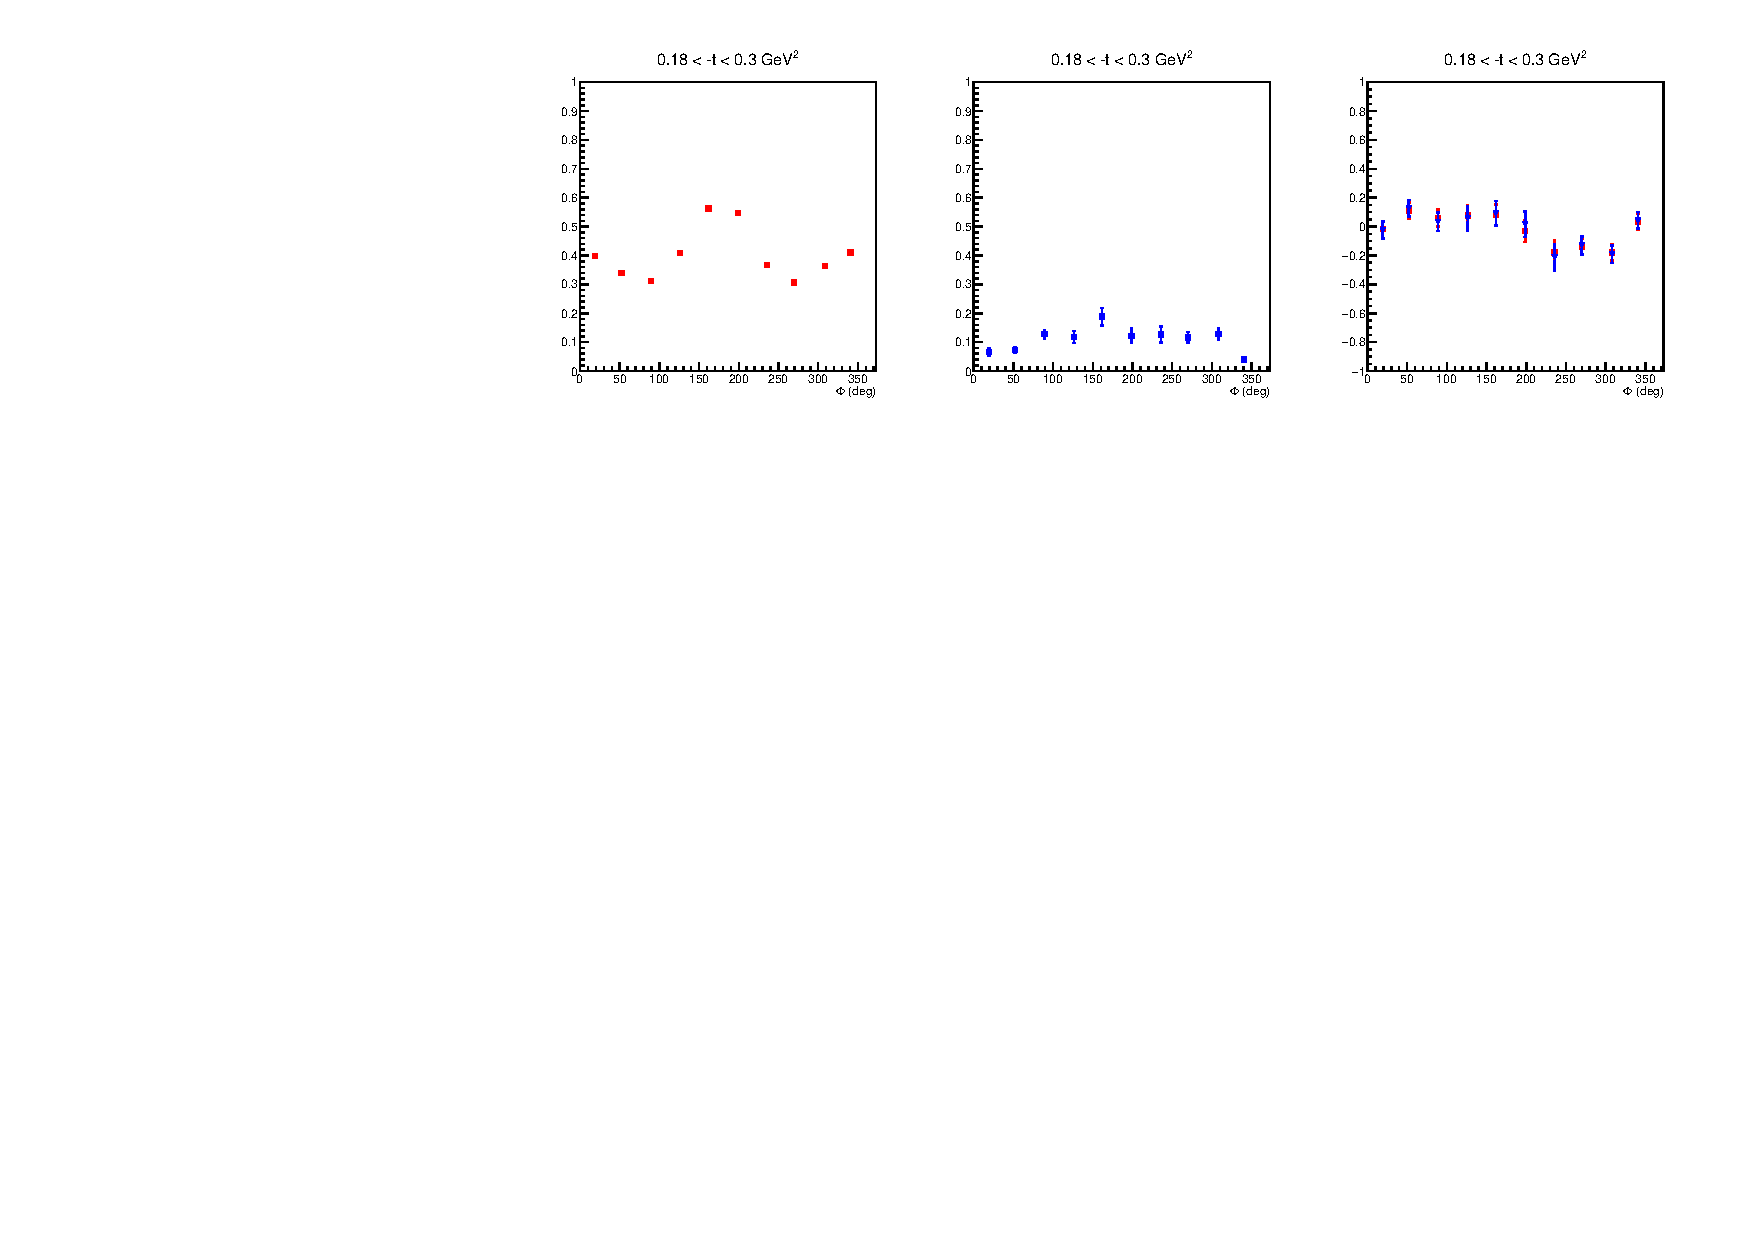
\includegraphics[width=140mm]{pi0_cont_tsa.pdf}
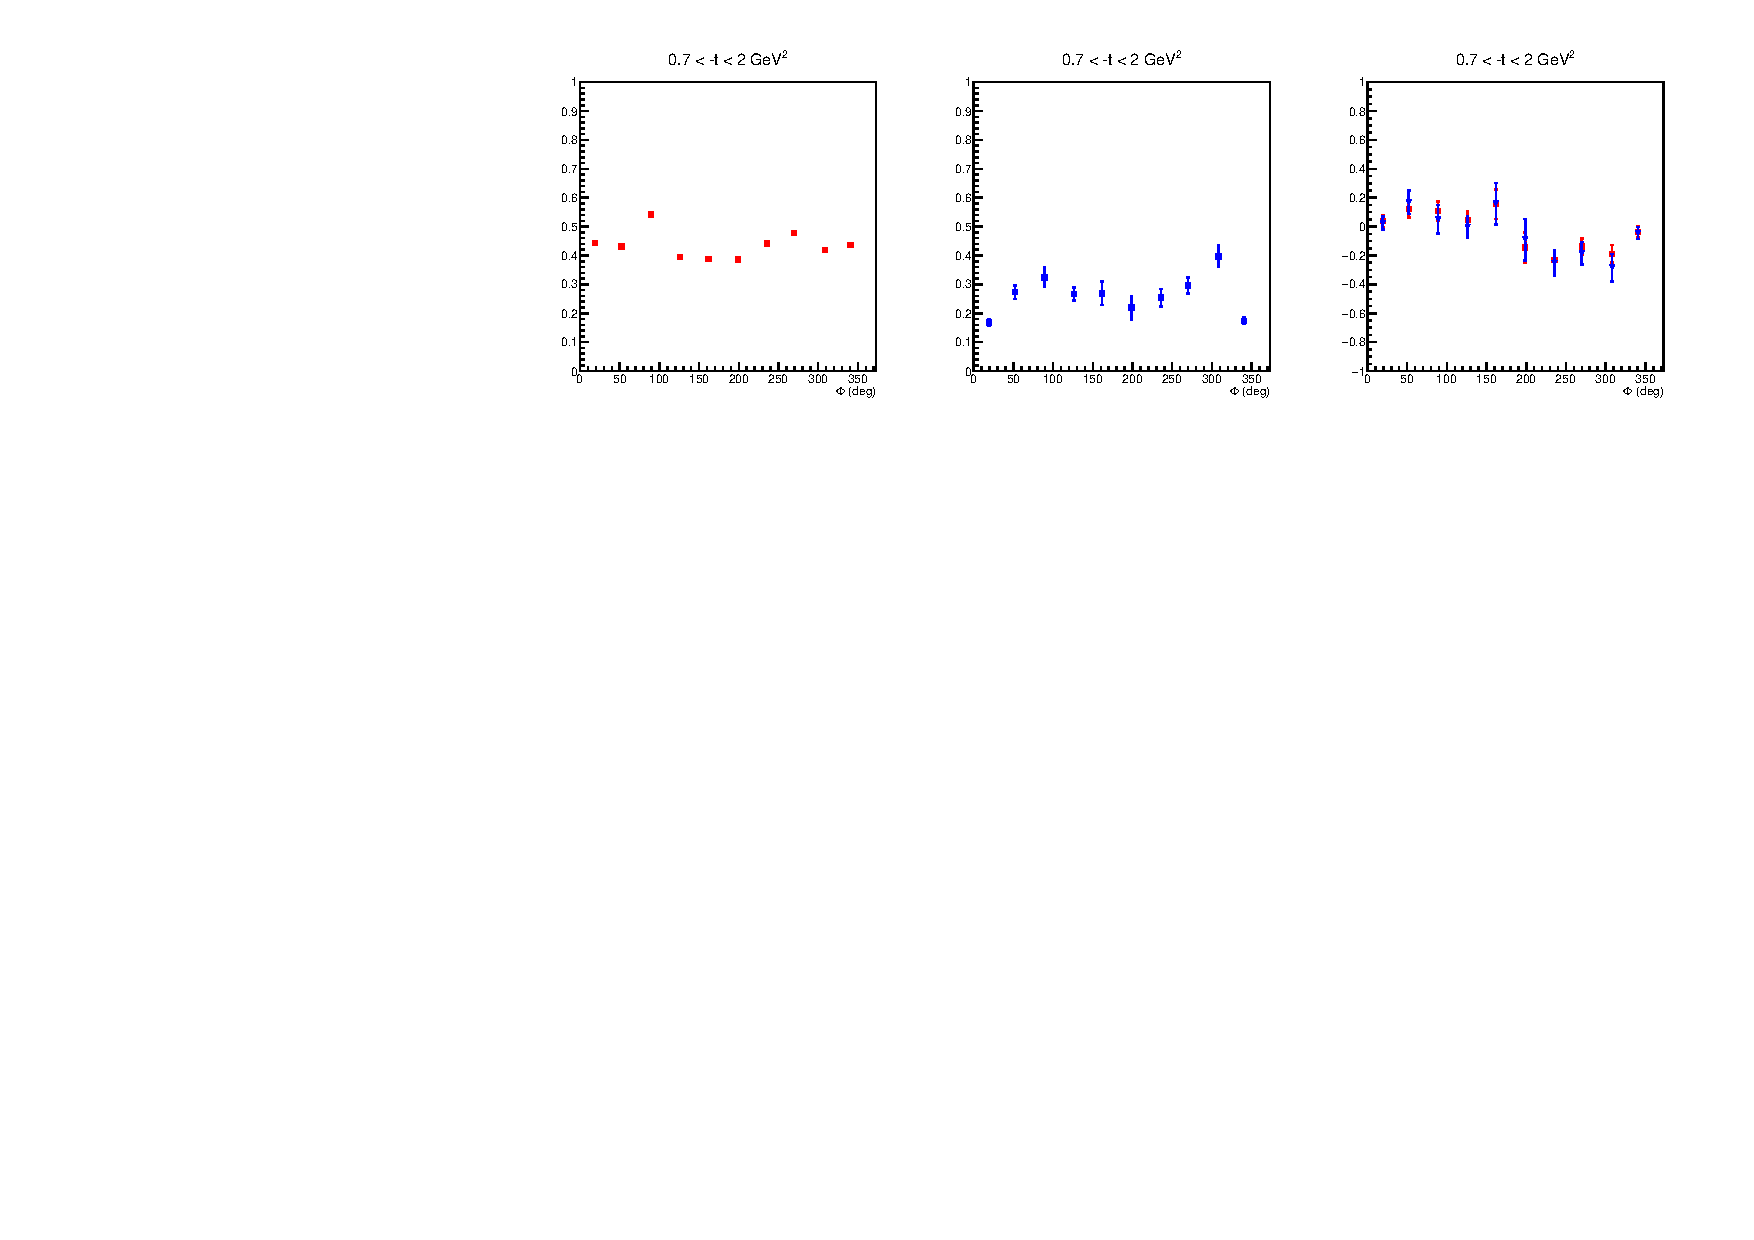
\includegraphics[width=140mm]{bin_q20_xb3_t3.pdf}
\caption [pDVCS results from the eg1-DVCS CLAS dataset]
{Plots from the proton-DVCS analysis of the eg1-DVCS CLAS dataset \cite{pisano}, for two different kinematic bins (top and bottom). Left: Acceptance ratio "$\frac{1 \gamma}{2 \gamma}$"; middle: $\pi^0$ contamination fraction; right: target-spin asymmetry before (red) and after (blue) $\pi^0$ background subtraction.}
\label{pi0_eg1dvcs}
\end{center}
\end{figure}
%
The proton-DVCS analysis of the eg1-dvcs NH$_{3}$ dataset showed that a combination of optimized cuts on the exclusivity variables, designed to minimise the background, and the simulation- and data- based subtraction of Eq.~\ref{pi0_formula} to remove the remaining contamination was a sound technique. In terms of systematics, the asymmetries were minimally affected even when the background estimation was artificially varied by 30\%. This is important also because it shows how little this procedure depends on the Monte-Carlo model adopted. 

\section{Dilution factor}\label{sec_dilution}
For both the nDVCS and $en\pi^0$ final states, dilution factors are necessary to correct the experimental yields for the contribution from the scattering on the unpolarized nitrogen of ND$_3$. The dilution factor, that will be determined using data taken on ND$_3$ and on ${}^{12}$C targets, is defined as
\begin{equation}
D_f = 1-c\cdot\frac{N_{{}^{12}{\rm C}}}{N_{{}^{14}{\rm ND}_3}} \label{eq_dilution}.
\end{equation}
Here, $N_{{}^{12}{\rm C}}$ is the number of events, normalized by the corresponding Faraday-cup counts, obtained from a carbon target and surviving all of the nDVCS (or $en\pi^0$) selection cuts, while $N_{{}^{14}{\rm ND}_3}$ is the number of events, likewise normalized and passing the same series of cuts, originating from ND$_3$. The factor $c$ accounts for the different luminosities of the two sets of data, which also take into account the different areal densities of the materials 
present at the target level for the two kinds of runs (ND$_3$ in the numerator, ${}^{12}$C in the denominator). 
For the eg1-dvcs experiment, it was found that the dilution factor, which, for pDVCS was determined to be around 0.9, does not display any sizeable dependence on any of the four kinematic variables describing the DVCS process. 
Adopting the same ratio as in eg1-dvcs, we estimate that acquiring ten times less events on ${}^{12}$C than on ND$_3$ should provide a sufficient count rate of carbon events to estimate the dilution factor at a satisfactory level of precision. A value of about 0.8 was obtained in recent studies of exclusive channels on ND$_3$, still using the eg1-dvcs dataset \cite{peter_exclusive}.
%As the dilution factor depends strongly on the exclusivity cuts, a conservative estimate of 0.7 is adopted for $D_f$ to produce the projected asymmetries of this proposal (Section~\ref{sec_countrate}). 

\section{Accidentals in the CND}\label{sec_accidentals}

In order to evaluate the rate of accidentals being reconstructed as a false neutron in the CND in coincidence with an $e\gamma$ event detected in CLAS12, GEMC simulations have been run in the following conditions \cite{raffa,proposal}: the primary electron has been generated going forward (to simulate the real hadronic event), plus 7500 other electrons have been thrown, distributed in a 124 ns window in bunches 4 ns apart, originating 10 cm upstream of the target. 7500 is approximately the number of beam electrons that would pass through our target in a 124 ns time window at the nominal CLAS12 luminosity. 124 ns is the typical time window of the DAQ expected for CLAS12, which corresponds to one event in CLAS12. These electrons then interact with the target itself, producing an electromagnetic and hadronic background hitting the neutron detector. The simulations were produced twice, using two different "physics lists" from GEANT4: electromagnetic plus hadronic processes ("EM-HAD"), and electromagnetic only (EM). The output of the simulations has been analyzed using the CND neutron-reconstruction algorithm. For each event, we selected the hit with the shortest time of flight which had a deposited energy above our chosen threshold (2~MeV) and below the maximum allowed time (9~ns). The reference time was chosen as that corresponding to the central beam bunch. Given the tight timing cuts that are imposed when reconstructing neutrons in the CND, we estimate that only slow neutrons ($p\sim 0.2$ GeV) from the previous bunch or photons from the following bunch could be accidentally registered as originating from the bunch in question. The momentum of the chosen particle is reconstructed assuming that it is a neutron, and cuts are applied on its momentum ($p_{min}= 0.2$ GeV/c) and on $\beta$ ($\beta<0.95$). Since previous simulations showed us that real neutrons should only produce at most one hit in one of the three layers of the CND, particles which had a second hit in another layer along the same trajectory were also removed. 
Figure~\ref{edep_background} shows the energy distribution of the background hits in the CND before any cuts are applied for the EM (top) and EM-HAD (bottom) cases. The latter has a more important tail at higher energies. 

\begin{figure}  
\begin{center}
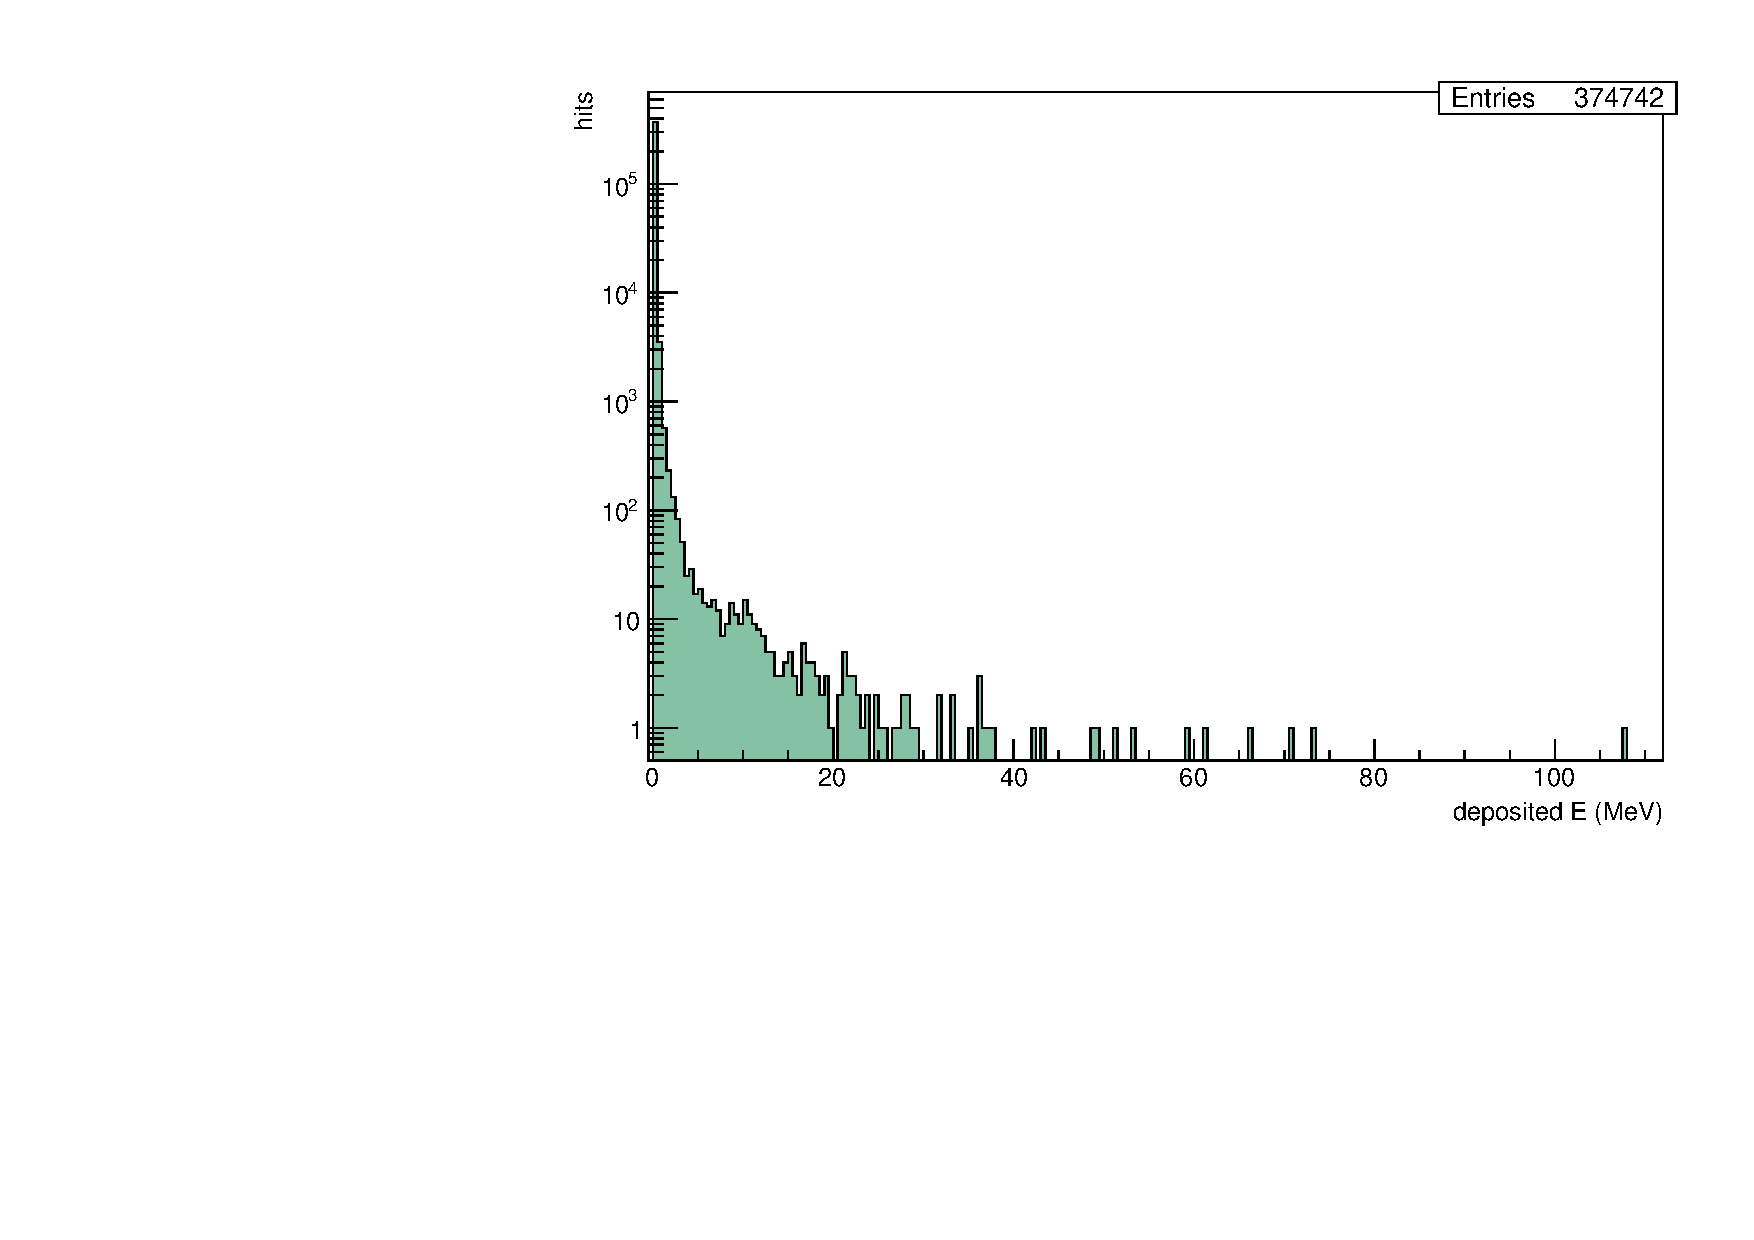
\includegraphics[width=100mm]{Egen_beforecuts_EMonly.pdf}
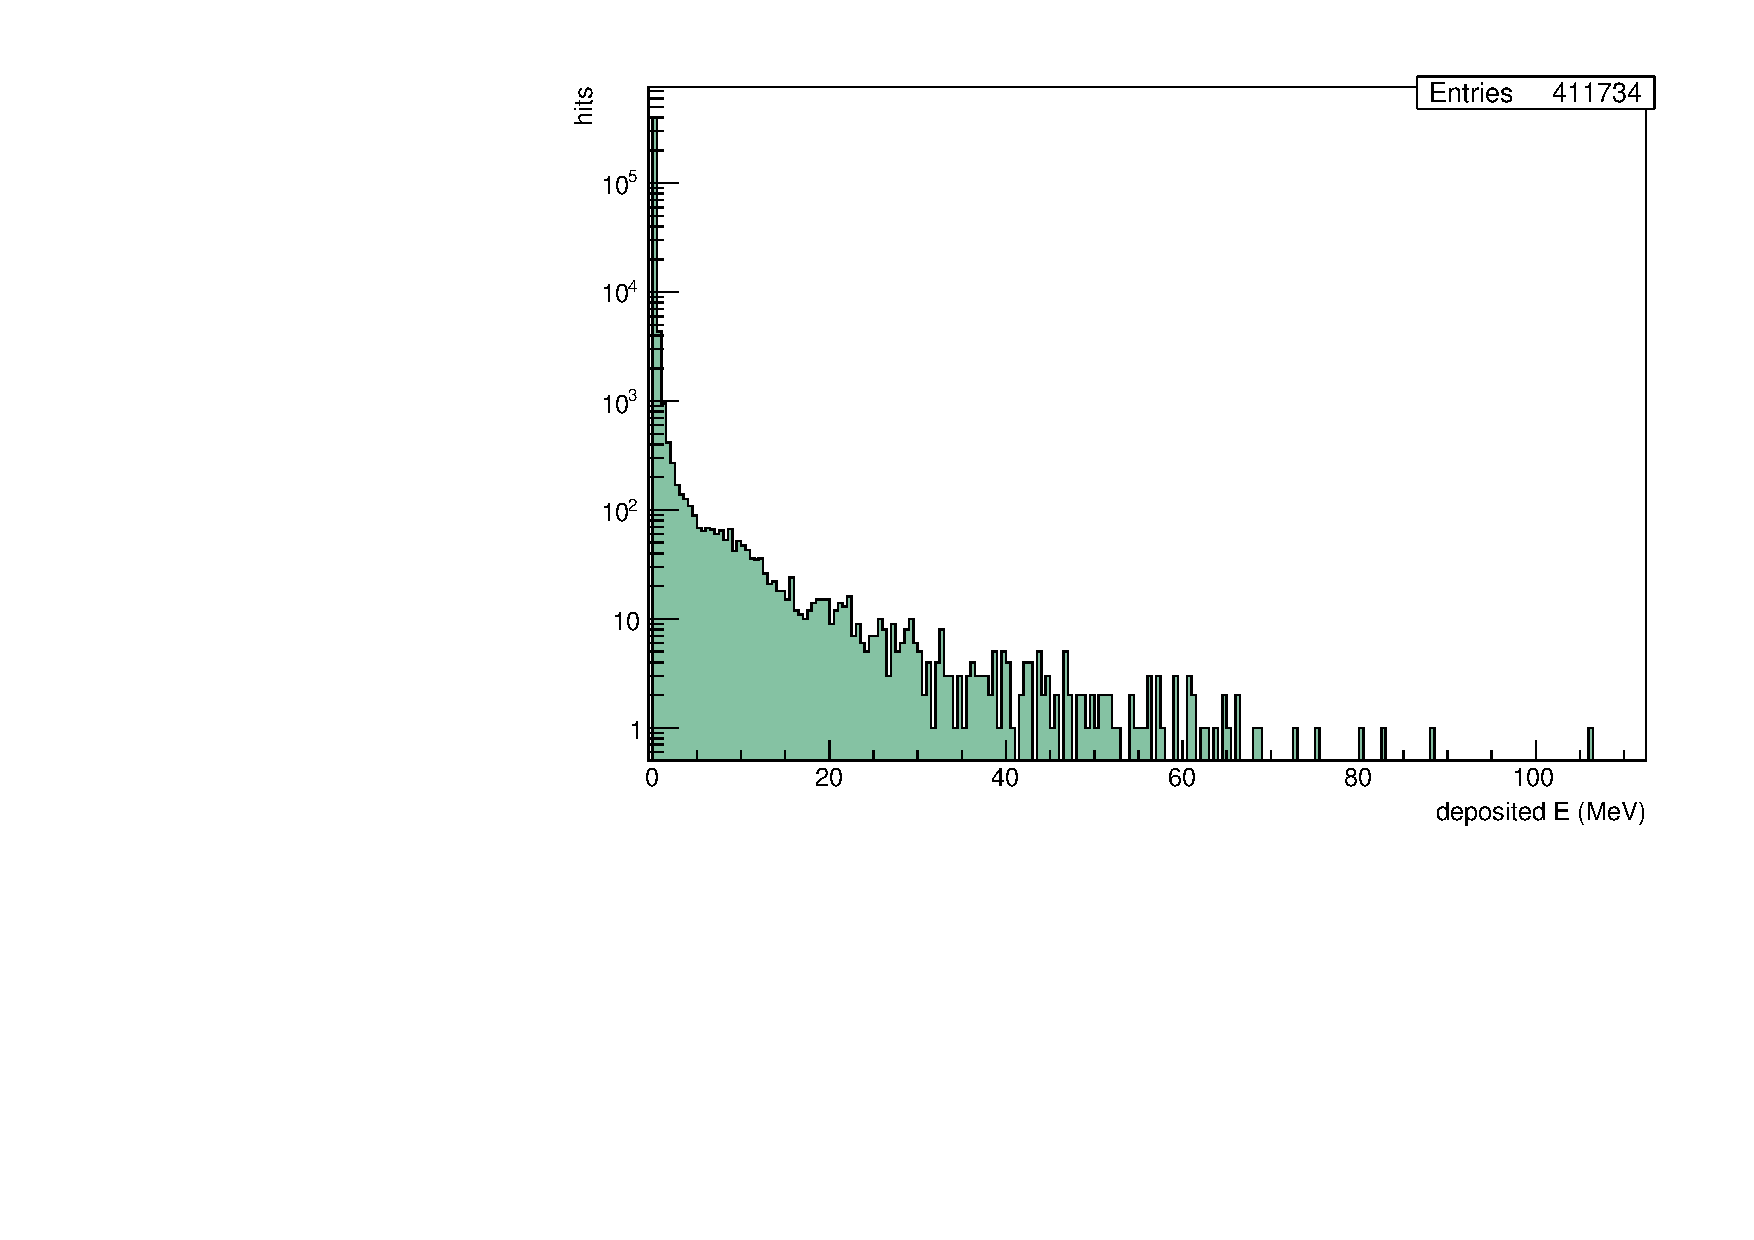
\includegraphics[width=100mm]{Egen_beforecuts_EMhad.pdf}
\caption []
{Energy deposited by the background hits in the CND, before cuts, as obtained with GEMC plus the EM physics list (top) and the EM-HAD one (bottom).}
\label{edep_background}
\end{center}
\end{figure}

The resulting probabilities that an event has a hit which passes the CND cuts are 0.0012 for the EM case and 0.01 for the EM-HAD case. Care must be taken in considering the EM-HAD probability, as there can be, on the one hand, double counting due to some of the simulated hadronic events producing actual triggers in CLAS12, and, on the other hand, uncertainties due to the GEANT4 parametrization of the physics list. The GEMC simulation of the whole CLAS12 and the full reconstruction software would be necessary to provide a more accurate estimate, but neither are available yet. The 0.01 of the EM-HAD case must therefore be regarded as a conservative upper limit. 
These hits can mimic a fake n-DVCS event by accidental coincidence with hadronic events where an electron and an energetic photon ($E_{\gamma}>2$ GeV) are detected in the forward part of CLAS12. The $e\gamma$ rate was estimated to be at most 50 Hz: the dominant process at play here is SIDIS with production of a $\pi^0$; the rate for such a process was estimated in \cite{sidis_prop} to be of 9 Hz (obtained by taking into account the factor of ~20 greater luminosity in the present experiment). Given that various kinematic cuts and the detection of both photons were required to produce that figure, we take a very conservative approach, assuming a rate for such events of the order of 50 Hz. This yields an accidental coincidence rate of the order of 0.06 Hz for the EM physics list, and 0.5 Hz for the EM+HAD physics list. These figures will be further reduced once the exclusivity cuts (Section~\ref{sec_excl_cuts}) will be applied, and will be therefore safely smaller than the expected rate for real $en\gamma$ events, which was estimated, with our event generators and FastMC, to be of 1 Hz for the present experiment. 

\section{Inclusion of the Forward Tagger}\label{ft_section}
In order to maximize the acceptance for forward-emitted photons, the compatibility of this experiment with the inclusion of the Forward Tagger has been studied. It must be noted that this detector is already part of the setup for the approved longitudinally polarized proton-DVCS experiment for CLAS12 \cite{E1206119}. 
The design of the beamline and of the shieldings, which protect the Drift Chambers of CLAS12 from the M\o ller background produced by the beam in the target, are currently undergoing modifications and studies. The goal of these studies is to optimize the shielding performances for the various experimental configurations that will be adopted with CLAS12. The current plan within the collaboration is to leave the Forward Tagger always installed in CLAS12, and to change the type of shielding between the target and the FT depending on whether or not the FT is used in the experiment. Figure~\ref{ft_shieldings}, produced with the interactive version of GEMC, shows the two designs of the M\o ller shielding in the ``FT on'' (top) and ``FT off'' cases. 
\begin{figure}[htbp] 
   \centering
   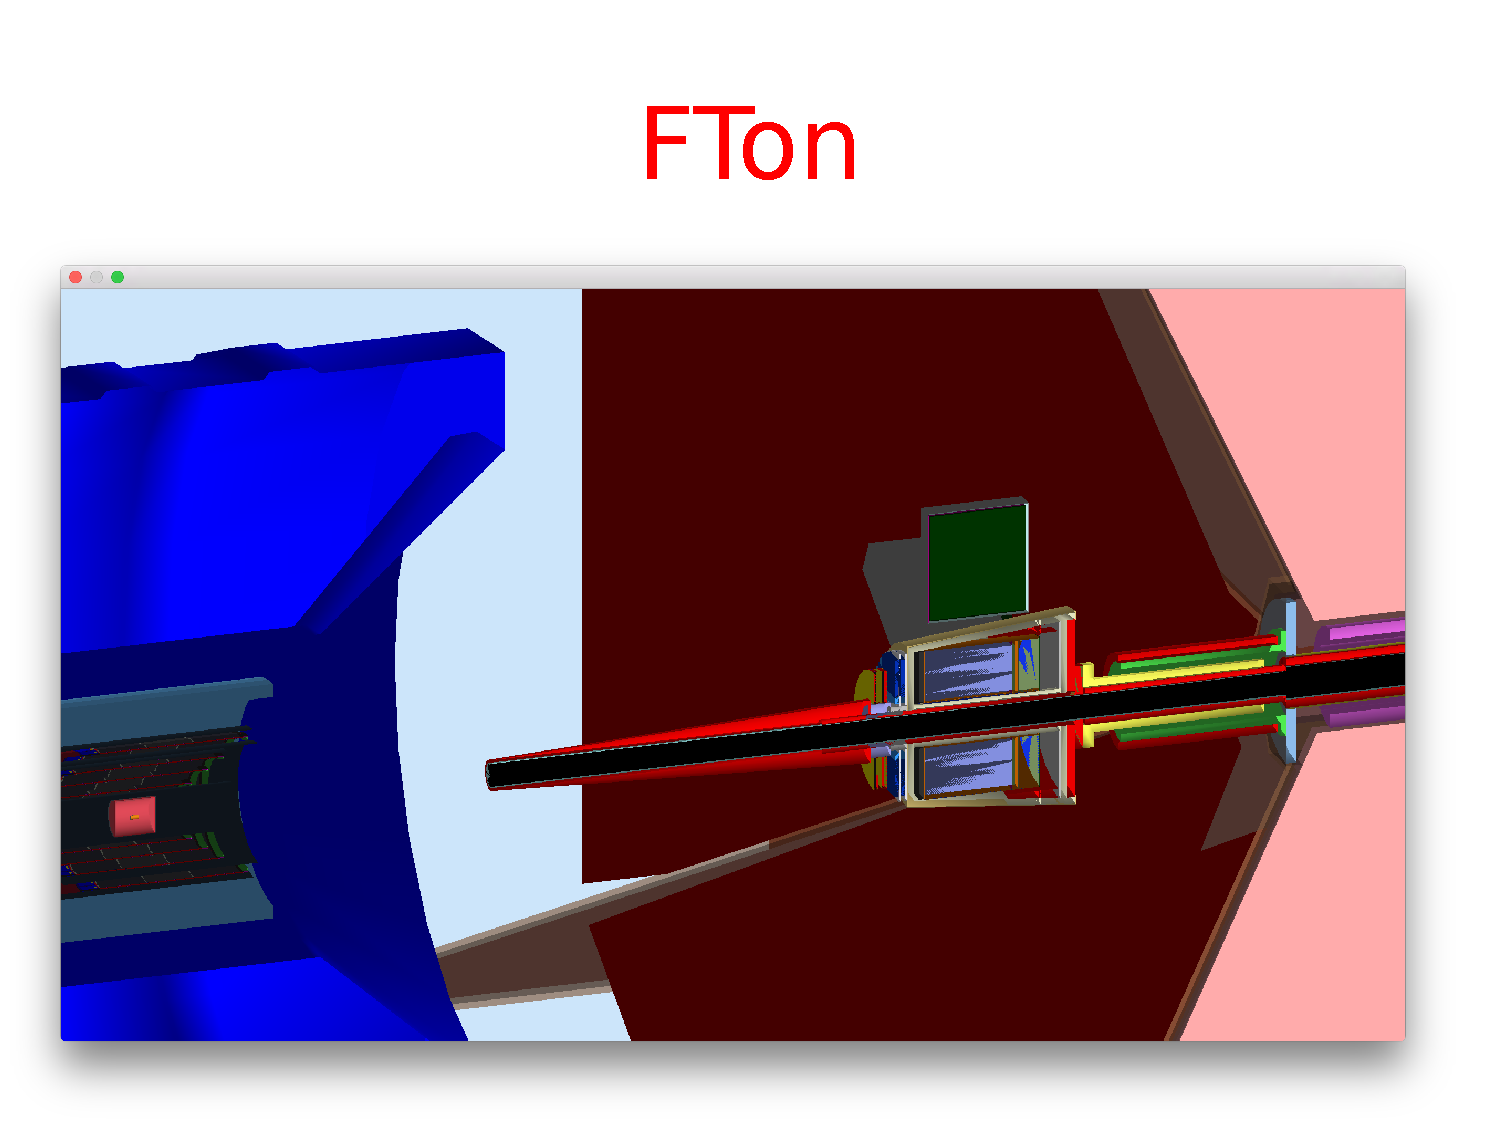
\includegraphics[width=4in]{FTon.pdf} 
   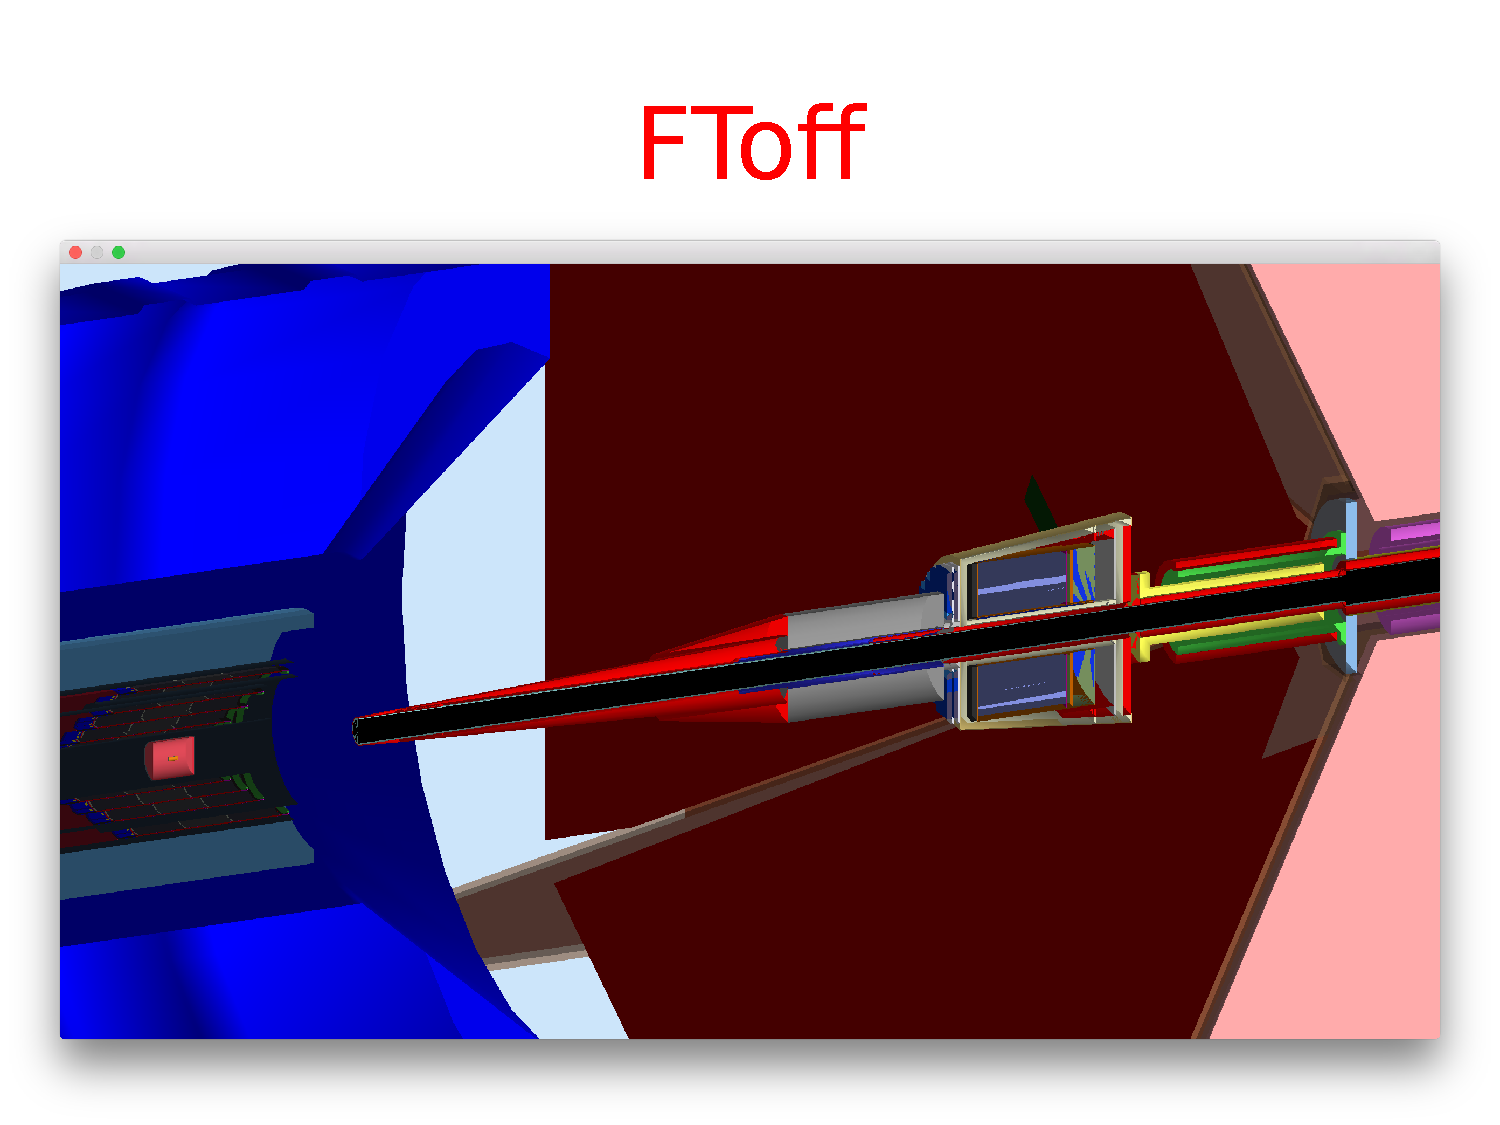
\includegraphics[width=4in]{FToff.pdf} 
   \caption{The CLAS12 M\o ller shieldings, for the ``FT on'' (top) and ``FT off'' (bottom) cases. When the FT is not used, a thicker shielding is adopted to minimize the radiation damage on the crystals.}
   \label{ft_shieldings}
\end{figure}
\subsection{DC occupancy and tracking performances at 10 nA}
Simulations were ran to test these designs, which have proven to be effective in keeping the M\o ller backgrounds low. Low background rates are necessary to ensure a high tracking efficiency. All the simulations tests performed until now were done for unpolarized targets, and thus the shieldings of Fig.~\ref{ft_shieldings} are optimized for such configuration. 
However, in the case of NH$_3$ or ND$_3$ polarized targets in order to minimize the radiation damage on the target the beam must be rastered over its surface, and this may induce higher background rates in the first region of the Drift Chambers, with respect to the unpolarized-target case. 
For the present proposal the GEMC simulation program was used to test the shieldings when the target is polarized and the beam is rastered. The polarized ND$_3$ target was implemented in GEMC as a cylindrical cell of teflon with diameter of 2.5 cm and length of 4 cm, filled with a mixture of 60\% ND$_3$ and 40\% liquid helium. The simulation was run with background events produced in a time window of 250 ns with a beam current of 10 nA, corresponding to 15625 electrons, rastered over a circular surface of 1.2 cm of radius. The four possible combinations of configurations (``with FT'', ``without FT'', ``with raster'', ``without raster'') were studied, for comparison purposes. Table ~\ref{tab:occupancy} shows the results for the occupancy in Region 1 (R1) for the four configurations, and Fig.~\ref{dc_occ} shows the occupancy for all regions of the DC for the ``with raster - with FT'' configuration, corresponding to the proposed experiment. 

\begin{table}[htbp]
   \centering
   \begin{tabular}{|c||c|} 
	\hline
      Configuration    & R1 Occupancy \\
	\hline
      FT + raster & 5.1\%\\
      FT + no raster & 2.3\%\\
      no FT + raster & 2.\%\\
      no FT + no raster & 1.8\%\\
	\hline
   \end{tabular}
   \caption{Occupancy for the first region of the CLAS12 drift chambers, obtained from GEMC simulations, for different configurations of the rastered beam and the Forward Tagger, for 10 nA of beam current.}
   \label{tab:occupancy}
\end{table}
\begin{figure}[htbp] 
   \centering
   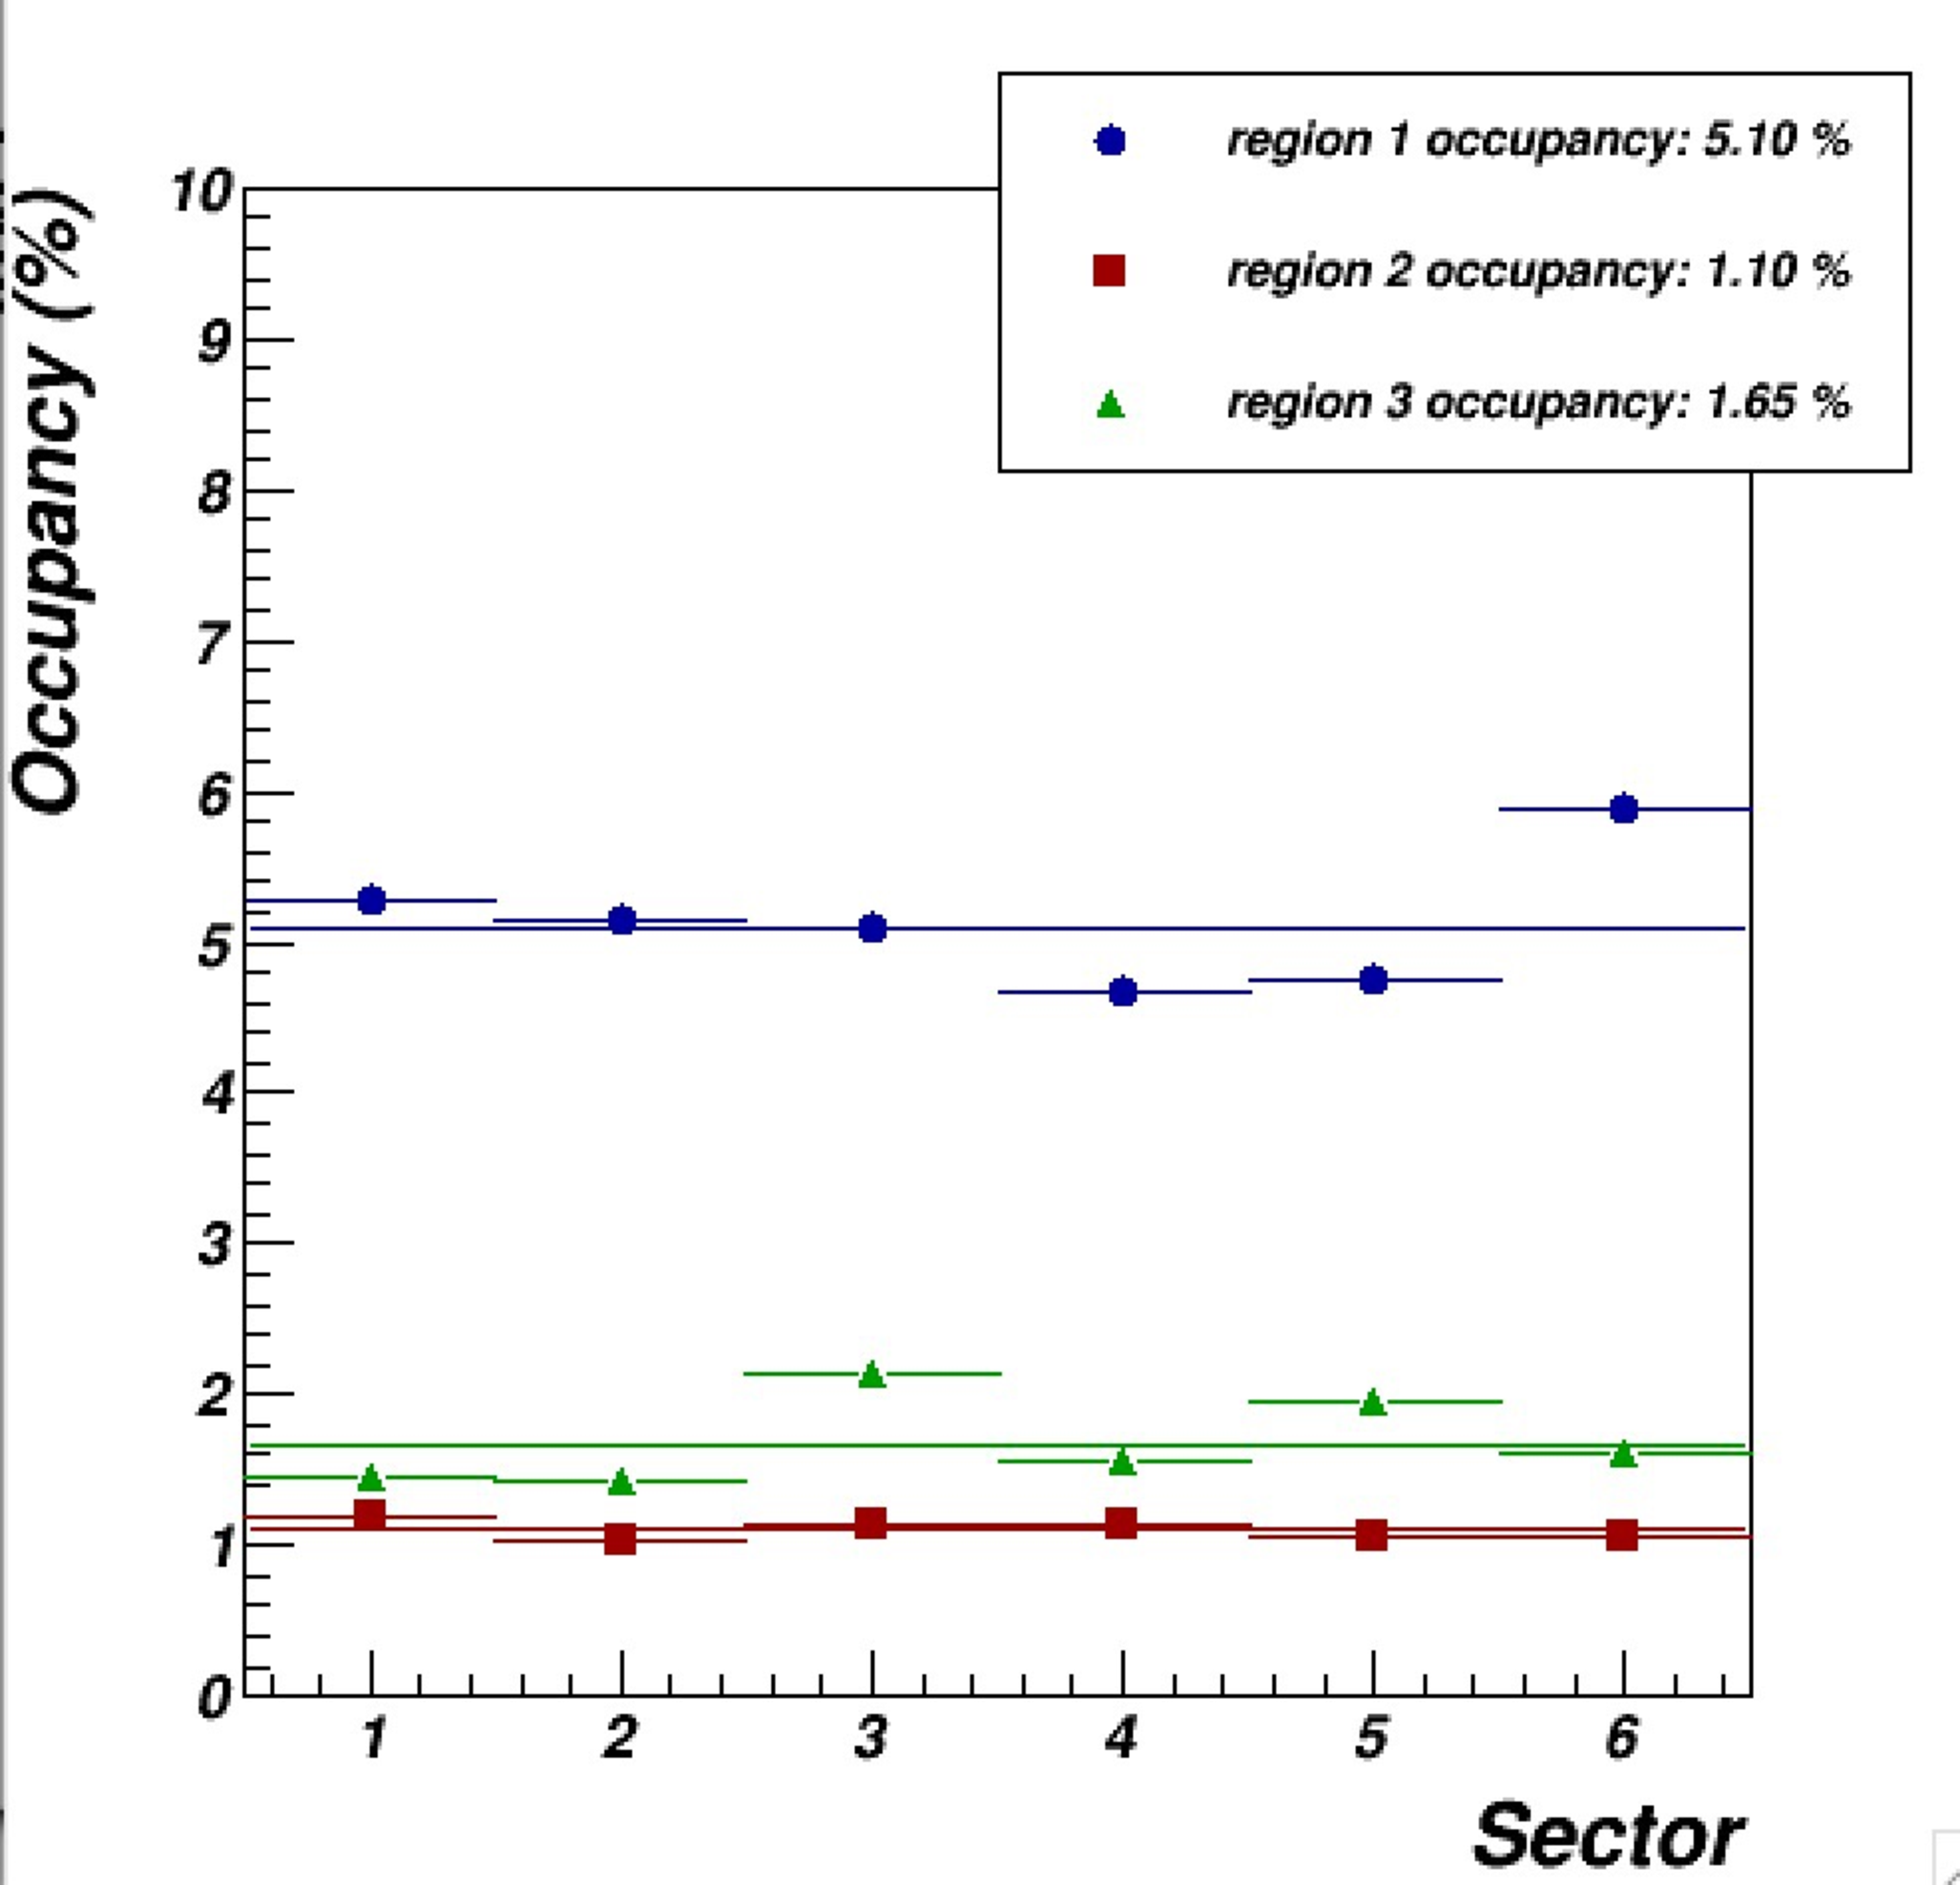
\includegraphics[width=4in]{Angela1.pdf} 
   \caption{DC occupancy, region-by-region, in each sector of CLAS12, for the configuration with FT and a rastered 10-nA beam on an ND$_3$ target.}
   \label{dc_occ}
\end{figure}
In the proposed configuration for this experiment, using this shielding, which is {\bf not yet optimized to be used with a rastered beam}, the DC occupancy is 5\% in region 1 and around 1\% in the other regions. In order to understand if such occupancies are tolerable for the CLAS12 reconstruction, the tracking efficiency was studied comparing the ``with FT'' and ``without FT'' cases (both with raster). This study was performed using GEMC simulations which included background as described in this Subsection, plus electrons generated at fixed kinematics ($p=4$ GeV, $\theta=15^{\circ}$, $\phi=0^{\circ}$). The CLAS12 reconstruction was run over the simulated files, and the tracking efficiency, for both Time-Based Tracking (TBT) and Hit-Based Tracking (HBT), was estimated for the two configurations. Table~\ref{track_eff_table} summarizes the results. 
\begin{table}[htbp]
   \centering
   \begin{tabular}{|c||c||c|} 
	\hline
      Configuration    & HBT efficiency & TBT efficiency \\
	\hline
      FT + raster & 94\% & 85\%\\
      no FT + raster & 91\% & 90\%\\
	\hline
   \end{tabular}
   \caption{Tracking efficiency, estimated analyzing GEMC simulations of single electron plus background, for the two configurations, ``with FT'' and ``without FT'', for 10 nA of beam current.}
   \label{track_eff_table}
\end{table}
An example of a track that is correctly reconstructed in spite of the noise in R1 is shown in Fig.~\ref{tracking_eff}. 
\begin{figure}[htbp] 
   \centering
   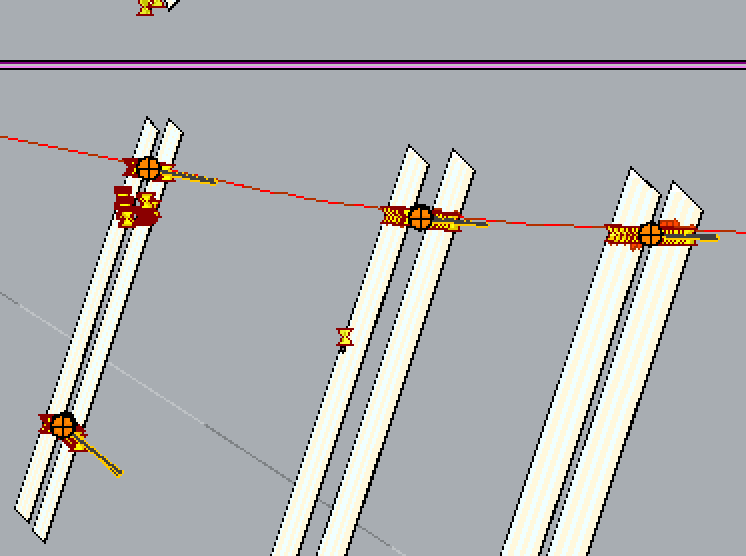
\includegraphics[width=4in]{RecoTrack.png} 
   \caption{Example of one electron track crossing the DCs for the configuration ``with FT - with raster'': the reconstruction works correctly in spite of the noise in R1.}
   \label{tracking_eff}
\end{figure}
There seems to be a 5\% decrease in TBT efficiency between the ``FT'' and ``no FT'' configurations. The higher HBT efficiency for the ``FT'' case could be due to the higher level of fake tracks in region 1. 
It must be pointed out that \cite{veronique_private}:
\begin{itemize}
\item{the shielding for the ``FT'' case is not yet optimized to be used with a rastered beam;}
\item{the tracking code is undergoing development;}
\item{with the current version of the code, the tracking efficiency for non-rastered beam and without any background is 95\%;}
\item{the cuts defining the TBT are not yet adapted to a rastered beam.}
\end{itemize}
The obtained momentum resolution for the 4-GeV electrons is shown in Fig.~\ref{mom_res}: it is 4 MeV, which corresponds to a $dp/p=1$\%, which is equal to the CLAS12 specifications. Thus, the results for the momentum resolution are encouraging. 
\begin{figure}[htbp] 
   \centering
   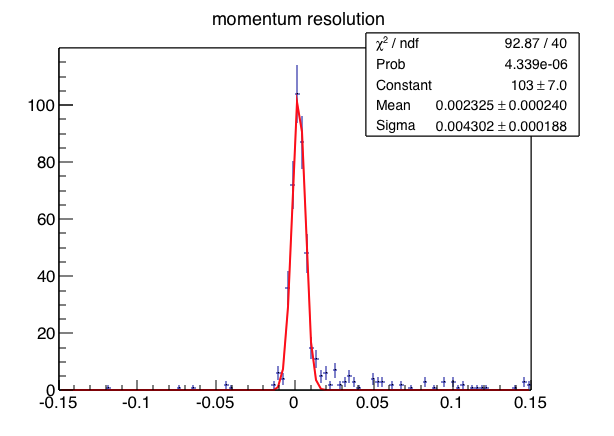
\includegraphics[width=4in]{mom_res_raster.png} 
   \caption{Momentum resolution for simulated 4-GeV electrons, plus background, in the ``with FT'' configuration. }
   \label{mom_res}
\end{figure}
All this considered, it is not fully clear, at the present stage, if a satisfactory tracking efficiency can be obtained when the FT is used and a 10-nA beam is rastered over the ND$_3$ target. %It must also be noted that the EC will also be used for electron identification and measurement of its kinematics. Assuming, as a worse-case scenario, that the current DC tracking efficiency performances were not improved, it could still be possible to use the HBT information coupled to the one from the EC to ensure proper measurement of the electron. 
%and it is not yet clear at this stage what the limit is for the acceptable DC occupancy in CLAS12 to ensure proper tracking, as the tracking reconstruction software is still under development. Preliminary studies \cite{procureur} suggested that tracking should be possible with DC occupancies up to 8-10\%. A definitive answer on this issue can only come when CLAS12 commissioning data will be taken at different beam currents and analyzed with the appropriate tracking and reconstruction software. This proposal is based on the hypothesis that the Forward Tagger can not be used, for the above described reasons. However, if the tracking will prove to be feasible at such levels of DC1 occupancies, the introduction of the Forward Tagger in the setup of this experiment could be beneficial (see Section \ref{sec_countrate} to see the projected asymmetries with and without inclusion of the FT).
\subsection{Radiation dose and backgrounds on the Forward Tagger}
The GEMC simulations containing only the background, for the ``with FT - with raster'' configuration were also used to test the background levels on the Forward Tagger. Figure~\ref{FT_dose} shows the radiation dose (in rad/h) on the crystals of the FT calorimeter. Even in the inner ``rings'', where the backgrounds produced by the beam are at their highest, the dose does not exceed 5 rad/h, which is below the limits of tolerance of the crystals that were selected to be part of the FT \cite{fegan_FT}. 
\begin{figure}[htbp] 
   \centering
   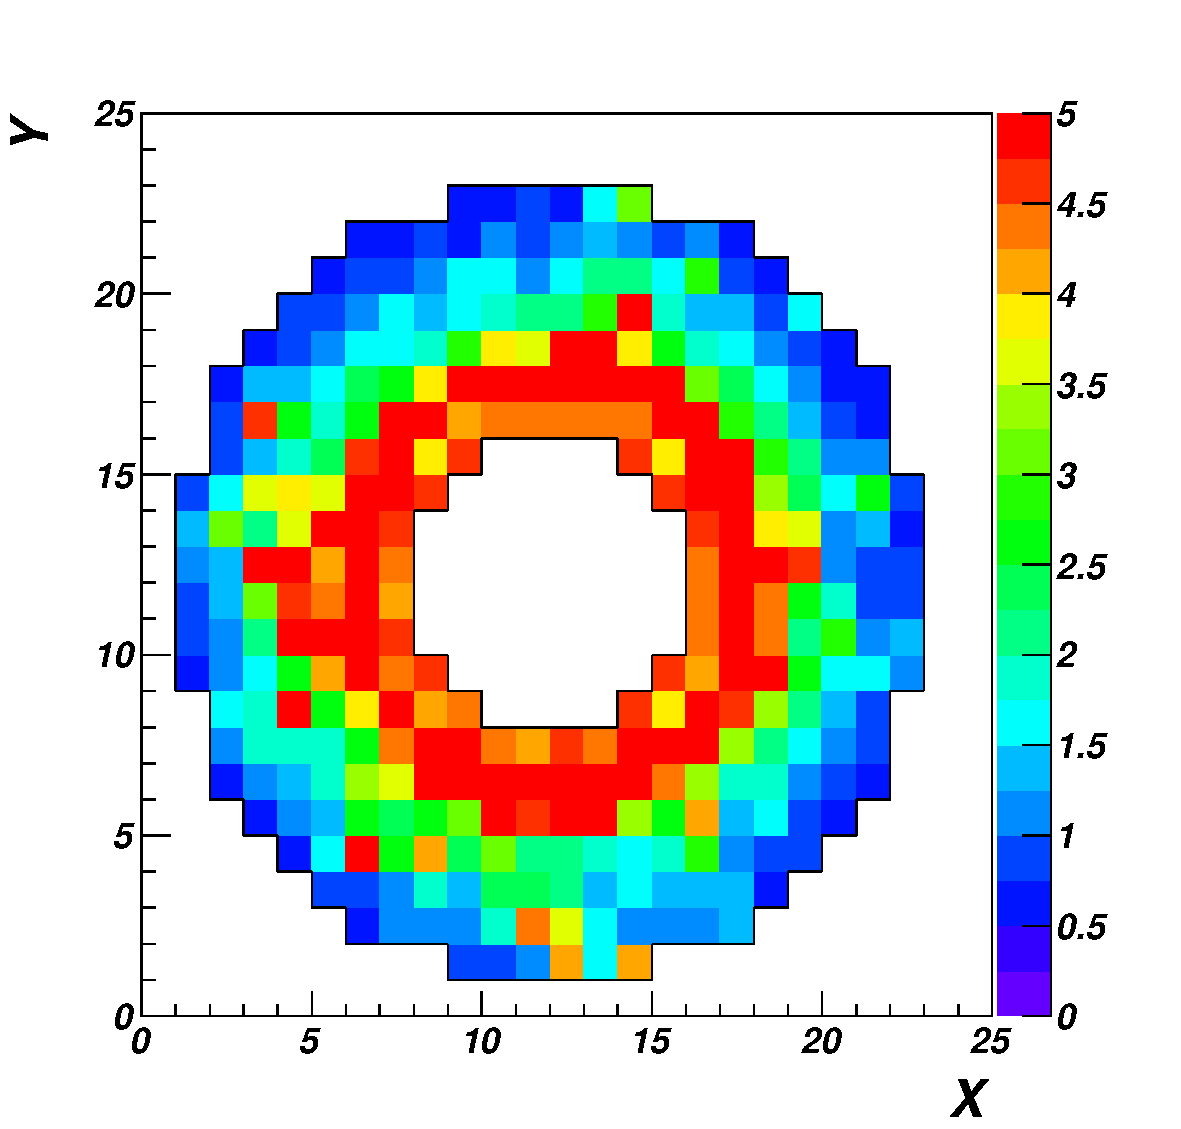
\includegraphics[width=4in]{ft_rad.pdf} 
   \caption{Radiation dose on the FT crystals, obtained from the GEMC background simulations, for the configuration ``with FT - with raster''. The units along $z$ are (rad/h).}
   \label{FT_dose}
\end{figure}
The average energy deposited by the background in the crystals per event was computed integrating over a time window of 120 ns, and it is shown in Fig.~\ref{ft_time}: it is at most around 10 MeV. 
\begin{figure}[htbp] 
   \centering
   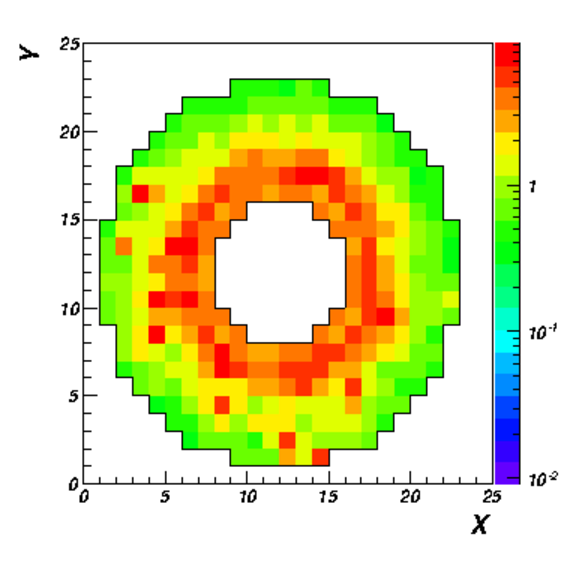
\includegraphics[width=4in]{ft_time.pdf} 
   \caption{Average energy deposit per event in the crystal of the Forward Tagger, obtained with the GEMC background simulations, for the configuration ``with FT - with raster''. The units along $z$ are MeV. }
   \label{ft_time}
\end{figure}
Considering that the typical energies of the photons that will be selected as DVCS candidates are above 2 GeV, the background levels in the FT do not seem critical. 

\subsection{Inclusion of Forward Tagger at 5 nA}
In conclusion, the results of the simulations carried out until now are that if the FT is used with the a 10-nA rastered beam, with the present shielding design, which is not optimized for this setup, and version of the tracking code, the FT itself would not have major problems, but there would be about 5\% of loss in tracking efficiency due to the noise in region 1 of the DC. As the design of the shielding can be further improved for the case in which the beam is rastered, and the tracking algorhytms are also under development, we are hopeful that an optimal configuration will be found that could allow the use of the FT at high luminosity, for the whole duration of the run-group extension. 
However, to be on the safe side, given, on the one hand, the results of the simulations at today, and, on the other hand, the very high cross section that DVCS/BH events have in the kinematics covered by the FT ($\phi\sim 0^{\circ}$ and $\phi\sim 360^{\circ}$), the following plan is adopted for this extension proposal:
\begin{itemize}
\item{run for 50 days at full luminosity (corresponding to 10 nA of beam current) without the Forward Tagger, and}
\item{run for 10 days at half luminosity (5 nA) with the Forward Tagger.}
\end{itemize}
Figure~\ref{dc_occ_5nA} shows the DC occupancies for the FT+raster configuration, with 5 nA of beam current. The value for R1 is low enough to ensure tracking efficiencies above 90\% even with the currently non-optimized version of the reconstruction code. 
\begin{figure}[htbp] 
   \centering
   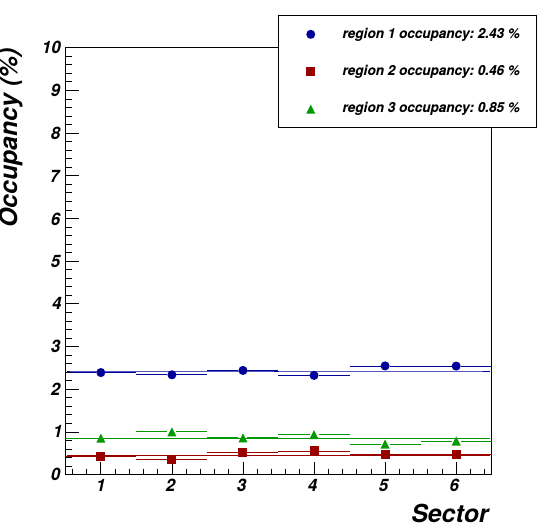
\includegraphics[width=4in]{dc_occ_5nA_FT_detail.png} 
   \caption{DC occupancy, region-by-region, in each sector of CLAS12, for the configuration with FT and a rastered 5-nA beam on an ND$_3$ target.}
   \label{dc_occ_5nA}
\end{figure}
 The following sections will show the expected results for the proposed experiment. 

 

\section{Projected results}\label{sec_countrate}
A GPD-based event generator for DVCS-BH on a deuterium target was run, assuming a luminosity of $3/20\cdot 10^{35}$ cm$^2$ s$^{-1}$ (where the factor $3/20$ accounts for the ratio of polarized neutrons to the total nucleons in ND$_3$) and a beam time of 100 days. The output of the generator was fed to the CLAS12 Fast-MC code, which included acceptance and resolution effects for CLAS12 and the CND. An additional factor of $10\%$ was also applied to mimick the efficiency of the CND for neutrons\footnote{Actually, this factor was adopted globally for ALL neutrons, even those falling within the EC acceptance. Given that the EC should have higher neutron efficiency than the CND, by at least a factor of 2, the projections for the count rates shown here are slightly pessimistic.}. nDVCS exclusivity cuts were then applied. This way, the expected yields for the $en\gamma(p)$ events produced on the ND$_3$ target were obtained. The kinematic space (in $Q^2$, $x_B$, $-t$, $\phi$) available with the acceptance of the CLAS12+CND setup was divided into the same 4-dimensional grid that was used for the unpolarized nDVCS proposal:
\begin{itemize}
\item{4 bins in $Q^2$, the limits of which are: 1, 2, 3.5, 5, 10 (GeV)$^2$;}
\item{4 bins in $x_B$, the limits of which are: 0.05, 0.15, 0.3, 0.45, 0.7;}
\item{4 bins in $-t$, the limits of which are: 0, 0.2, 0.5, 0.8, 1.2 (GeV)$^2$;}
\item{12 bins in $\phi$.}
\end{itemize}

The central kinematics for each bin were computed as weighted averages over the reconstructed events. The target-spin asymmetry and the double-spin asymmetry were then calculated as a function of $\phi$ using the VGG model (with input parameters $J_u=0.3$ and $J_d=0.1$) for each of the ($Q^2$, $x_B$, $-t$) bins that are kinematically allowed. 
Statistical errors were then obtained for these asymmetries using the approximated formula: 
\begin{equation}\label{error_asym}
\sigma_A = \frac{1}{P}\cdot \frac{\sqrt{1-P^2\cdot A^2}}{\sqrt{N}}.
\end{equation}
where $P$ is the polarization (and it is therefore equal to the target polarization for neutrons, $P_t$, for the TSA case, and to the product of beam and target polarizations, $P_bP_t$, for the DSA case), and $N$ is the expected yield in each 4-dimensional bin. % (Figs.~\ref{count_rate_1} and \ref{count_rate_2}). 

The resulting asymmetries with the associated expected error bars are shown in Figs.~\ref{fig_tsa_100_50_FT} (TSA) and \ref{fig_dsa_100_50_FT} (DSA). These same figures also show the comparison, for TSA and DSA, for running this experiment with either 50 or the proposed 110 days of beam time. 
The use of the Forward Tagger will improve the $\phi$ coverage at the edges ($\phi\to 0^{\circ}$ and $\phi\to 360^{\circ}$) for some of the low-$t$ bins, which is otherwise incomplete. This can be noticed in Figs.~\ref{fig_tsa_100_50_FT} and \ref{fig_dsa_100_50_FT}, where at the edges of several of the $\phi$ distributions only the black points are present. 

%For reference, the 4-dimensional acceptances obtained with the simulation are shown in Figs.~\ref{acceptance_1} and \ref{acceptance_2}. 

It is important to point out that the number of days chosen here (110) is the minimal amount of time necessary to be able to bin the TSA and the DSA in enough kinematic bins to describe in a satisfactory manner the dependence in all the 4 kinematic variables, while at the same time having statistical uncertainties not exceeding too much the ones expected for the BSA of E12-11-003 (Fig.~\ref{fig_bsa}). 

%\begin{sidewaysfigure}  
%\begin{center}
%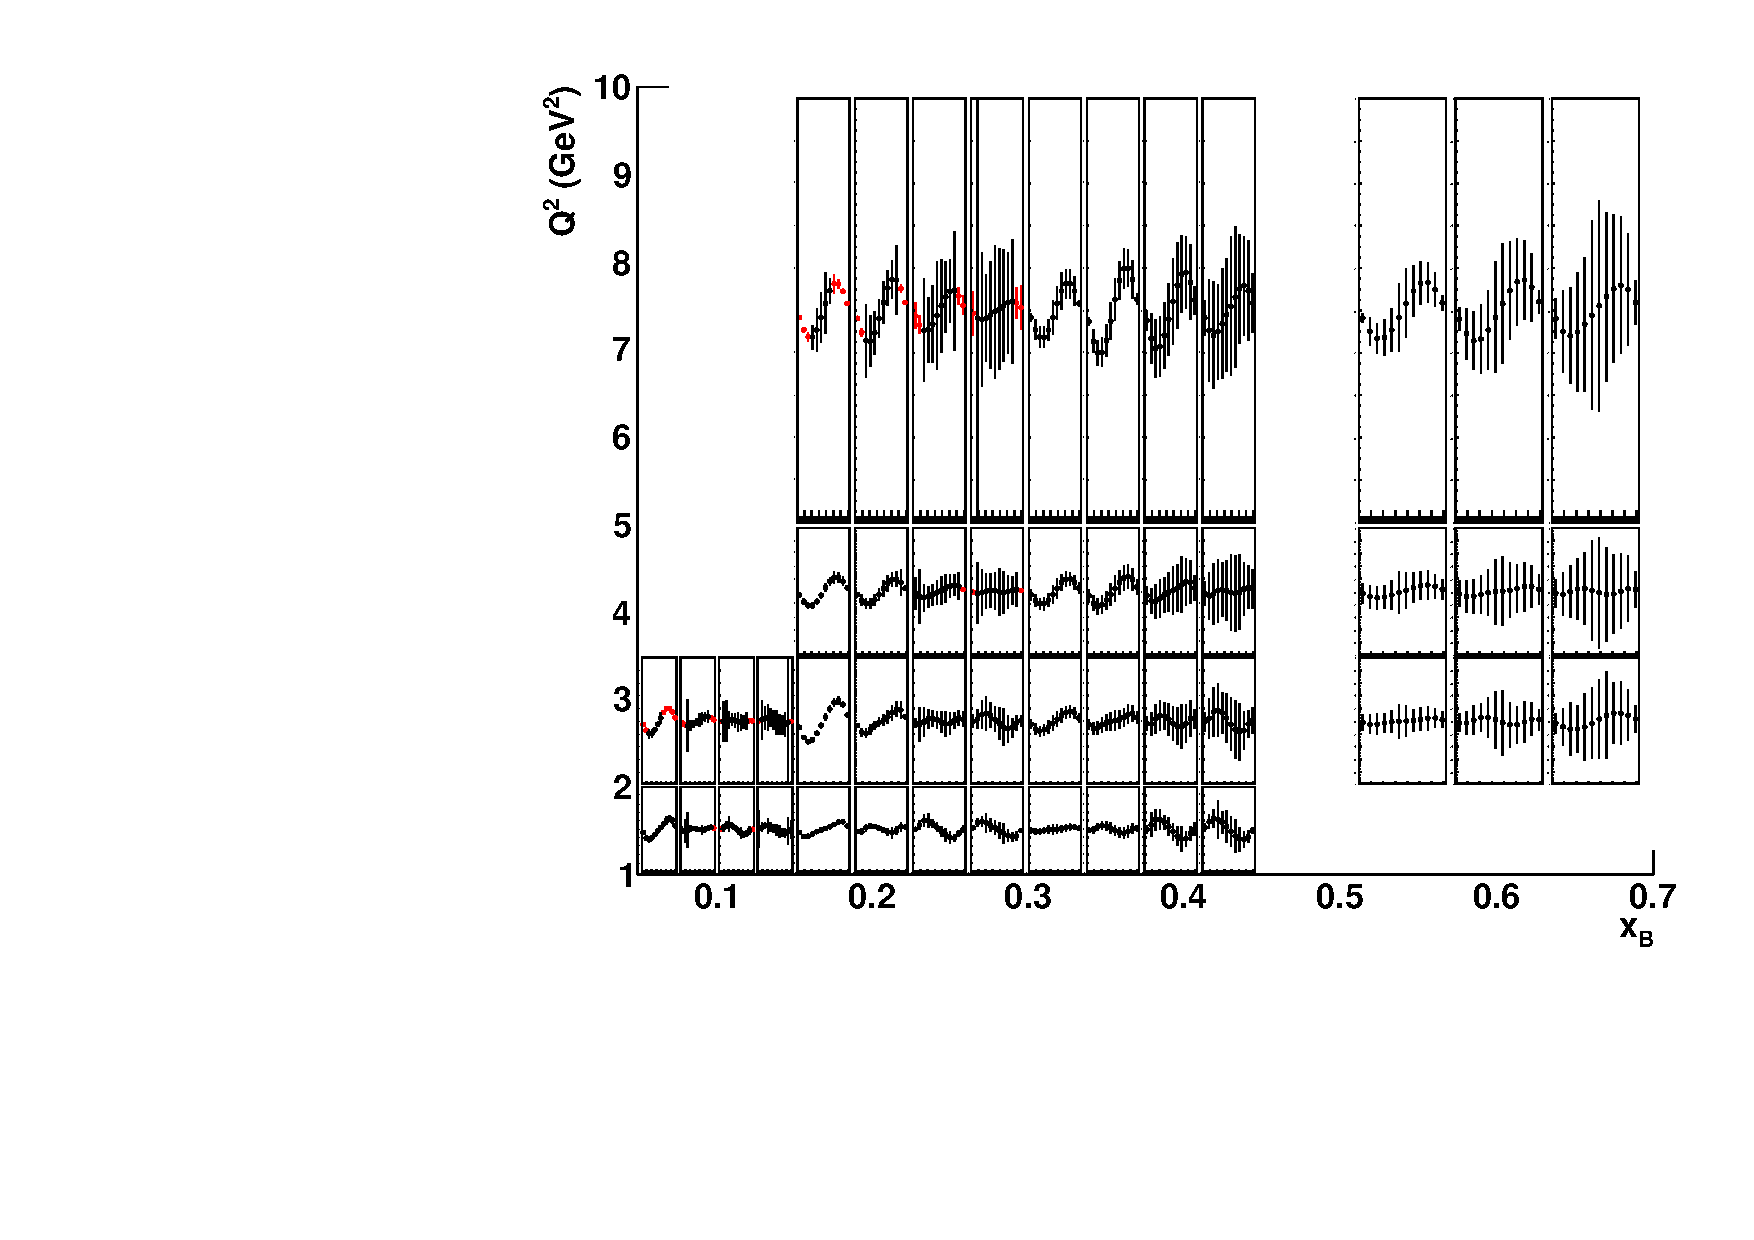
\includegraphics[width=200mm]{asym_polndvcs_tsa_newvgg_100days_FT_noFT.pdf}
%\caption[Projected target-spin asymetry]
%{Projected target-spin asymmetry. The y-scale range, common to all bins, is (-1;1). The black and red points are obtained, respectively, without and with the Forward Tagger. }\label{fig_tsa}
%\end{center}
%\end{sidewaysfigure}

\begin{sidewaysfigure}  
\begin{center}
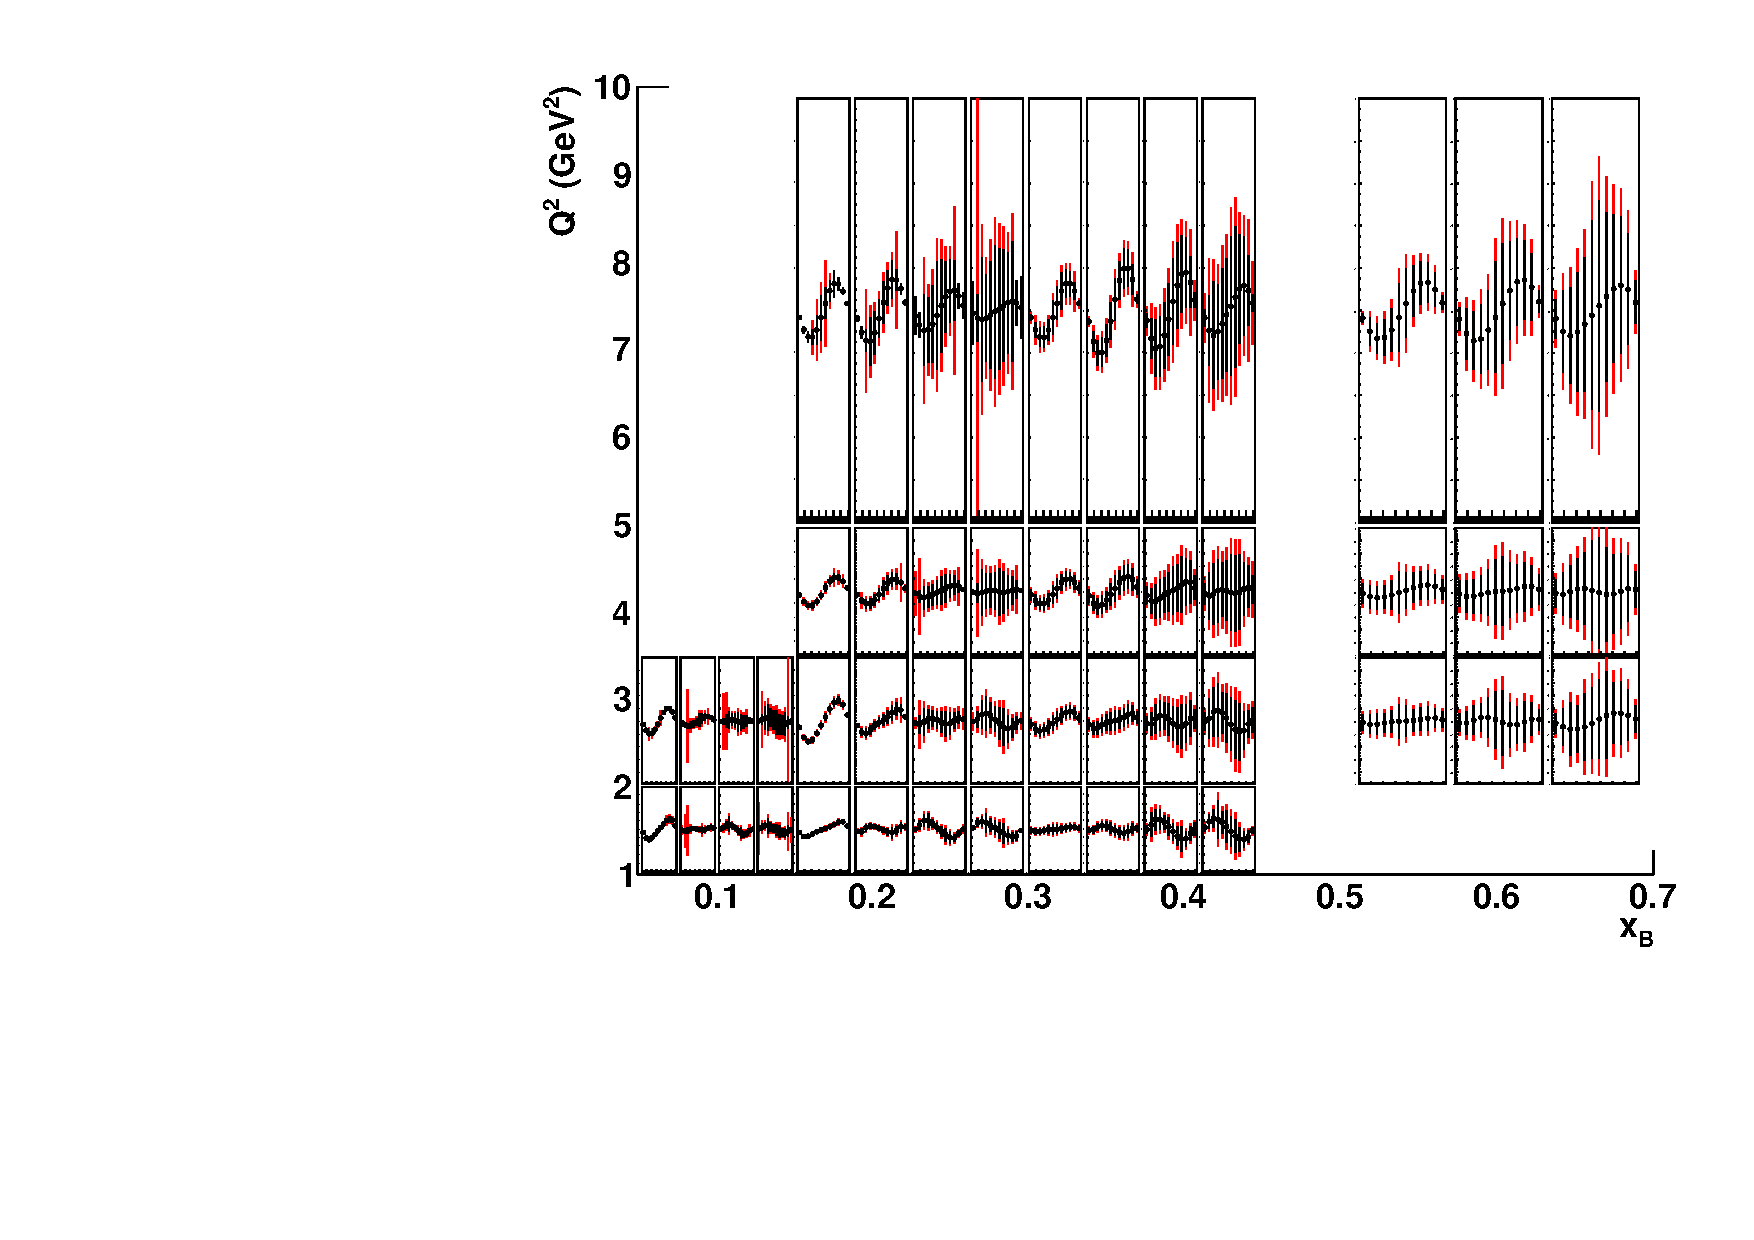
\includegraphics[width=200mm]{asym_polndvcs_tsa_newvgg_100_FT_and_noFT_50days.pdf}
\caption[Projected target-spin asymetry]
{Projected target-spin asymmetry. The y-scale range, common to all bins, is (-1;1). The black and red points are obtained, respectively, with 110 days and 50 days of beamtime.}\label{fig_tsa_100_50_FT}
\end{center}
\end{sidewaysfigure}

\begin{sidewaysfigure}  
\begin{center}
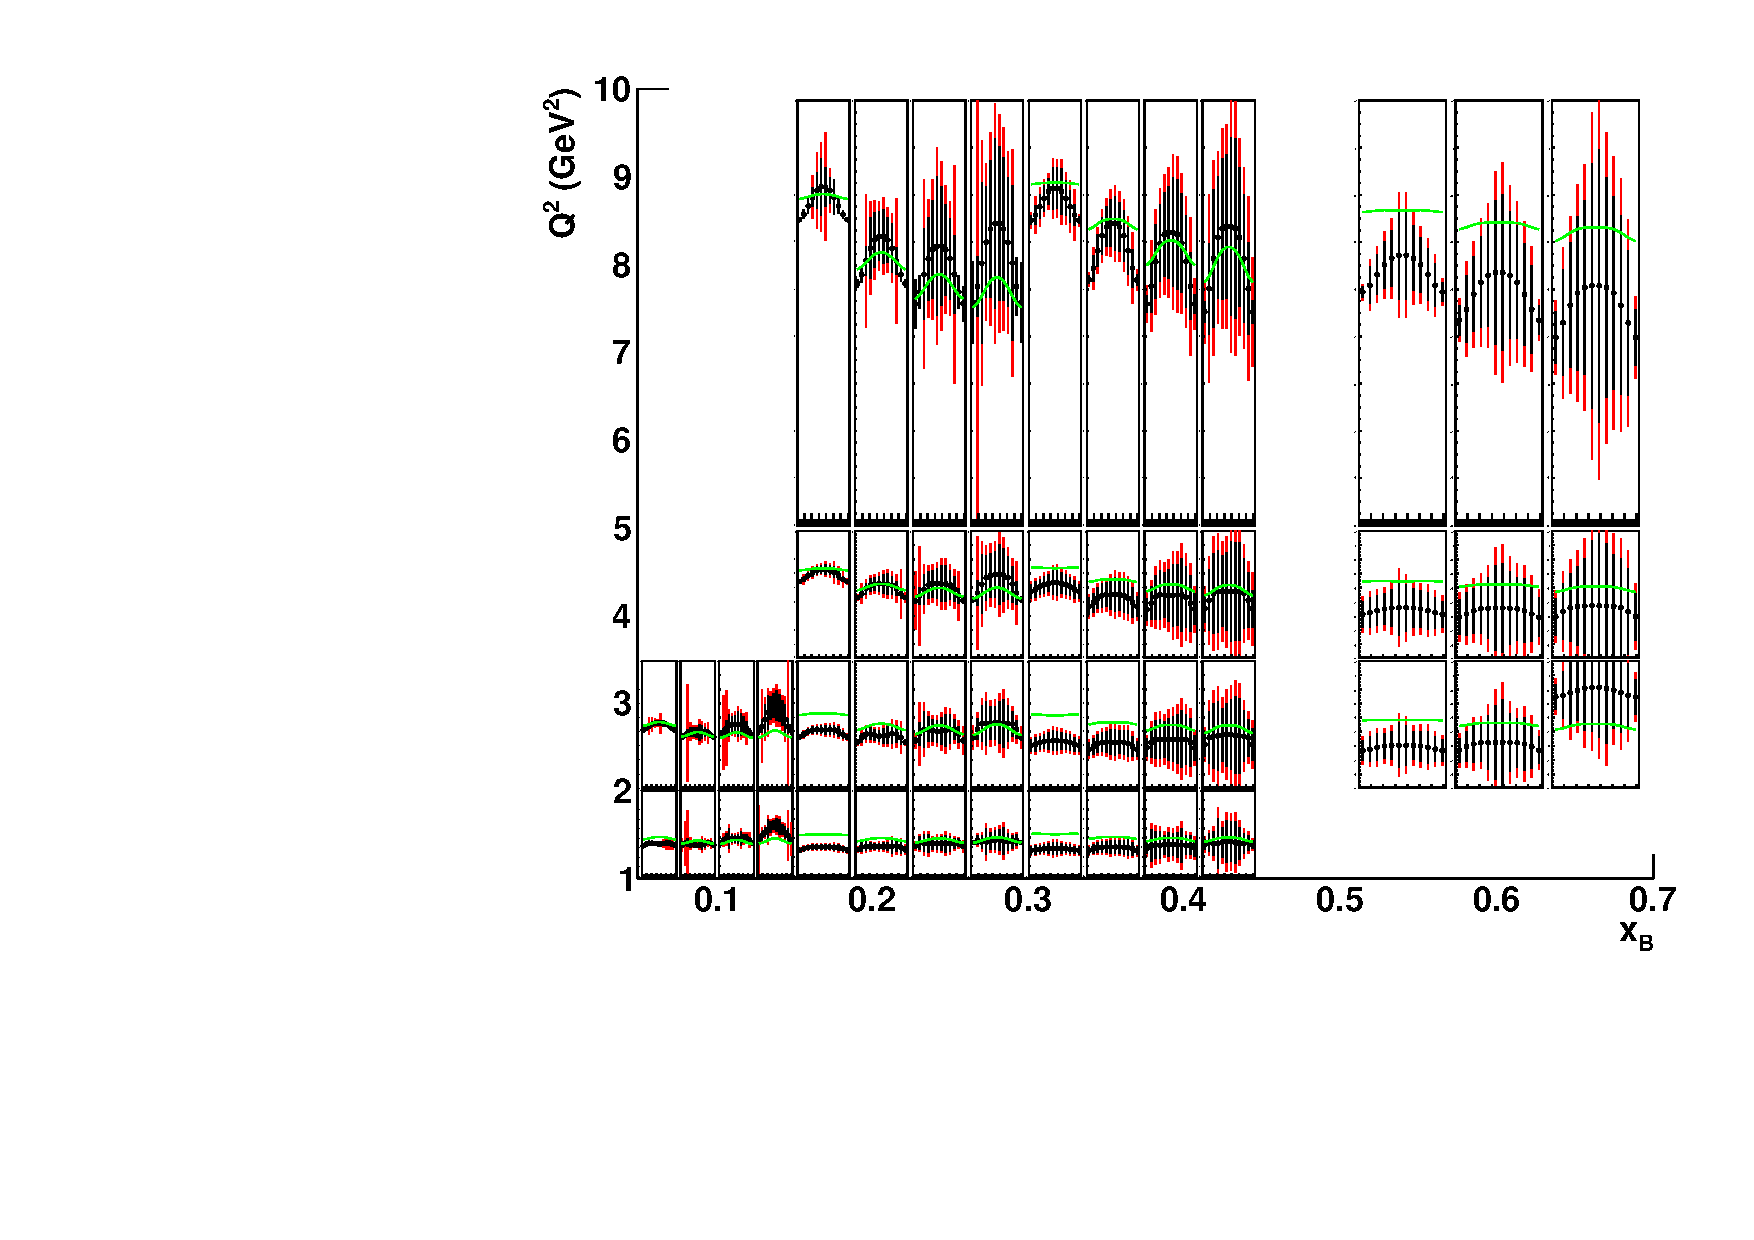
\includegraphics[width=200mm]{asym_polndvcs_dsa_newvgg_BH_100_50days_FT_and_noFT.pdf}
\caption[Projected double-spin asymmetry]
{Projected double-spin asymmetry, compared to the BH (green lines), calculated at the average kinematics of each bin. The y-scale range, common to all bins, is -0.6-1.2. The black and red points are obtained, respectively, with 110 days and 50 days of beamtime. }\label{fig_dsa_100_50_FT}
\end{center}
\end{sidewaysfigure}

\begin{sidewaysfigure}  
\begin{center}
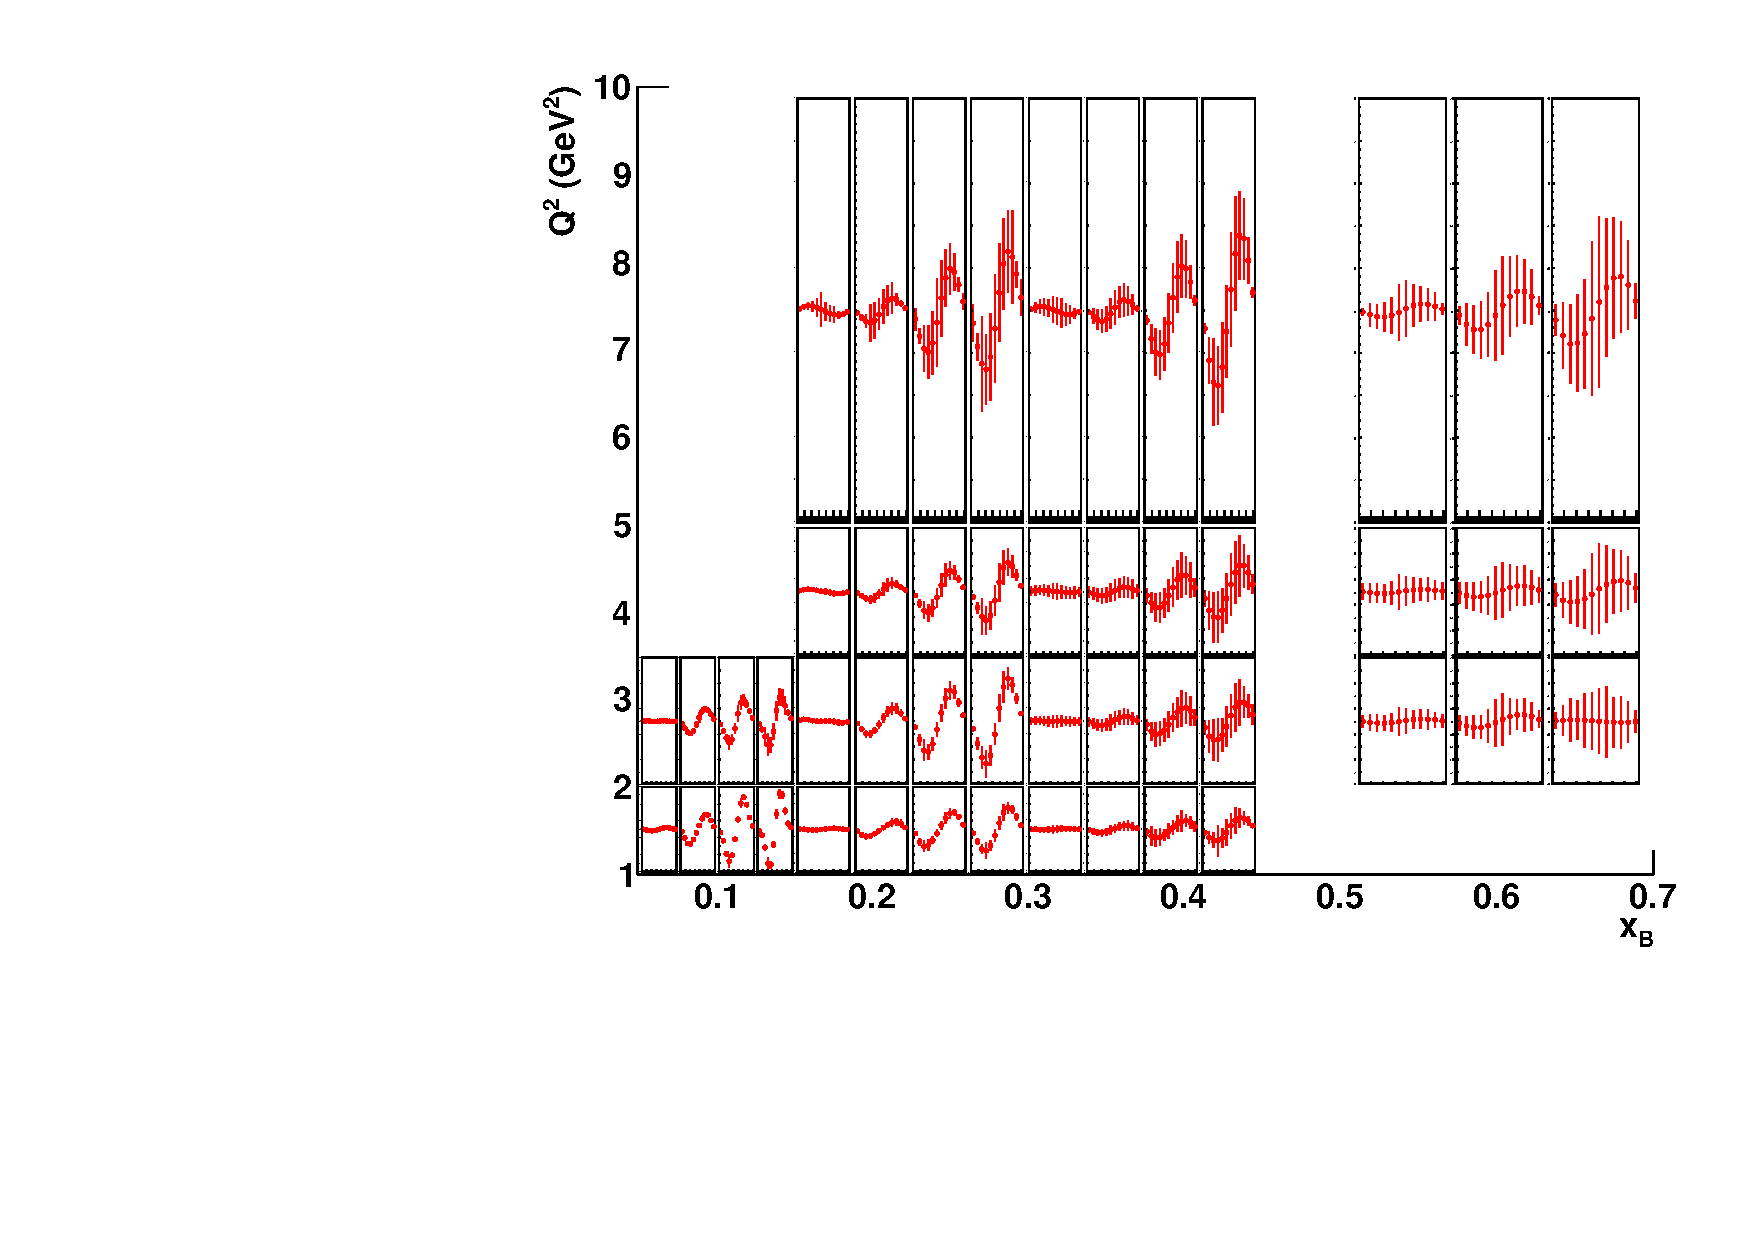
\includegraphics[width=160mm]{asym_newcuts_bsa_newvgg.pdf}
\caption[Projected beam-spin asymmetry from E12-11-003]
{Projected beam-spin asymmetry, as will be obtained from experiment E12-11-003 \cite{proposal}. The y-scale range, common to all bins, is -0.25-0.25.}\label{fig_bsa}
\end{center}
\end{sidewaysfigure}

\section{Extraction of Compton Form Factors}\label{sec_cff}
The three sets of projected asymmetries (BSA from \cite{proposal}, shown in Fig.~\ref{fig_bsa}, TSA and DSA from this work, Figs.~\ref{fig_tsa_100_50_FT} and \ref{fig_dsa_100_50_FT}, respectively) for all kinematic bins were processed using the fitting procedure described in Section ~\ref{sec_michel_fits} to extract the Compton Form Factors of the neutron.  
In the adopted version of the fitter code, $\tilde{E}_{Im}(n)$ is set to zero, as $\tilde{E}(n)$ is assumed to be purely real - it is parametrized in the VGG model by the pion pole $(1/(t-m^2_{\pi}))$. Thus, seven out of the eight real and imaginary parts of the CFFs are left as free parameters in the fit. A loose bound on the parameters is also applied, limiting them within the interval given by $\pm 5 \cdot {\rm VGG}$, where "VGG" stands for the prediction of the VGG model for the value of the CFF.

%The results for the 7 neutron CFFs are shown in Figs.~\ref{cff_him}-\ref{cff_etre}, as a function of $-t$, and for each bin in $Q^2$ and $x_B$. The points are the CFFs resulting from the fits, and their error bars reflect both the statistical precision of the fitted observables and their sensitivity to that particular CFFs. Only results for which the error bars are non zero, and therefore the fits have properly converged for that CFF, are included here. For comparison, three kinds of scenarios are shown: the blue points points show the CFFs that can be extracted with 100 days of beamtime, and using the FT for the 50 required by this extension; the black points show the CFFs that can be extracted with 100 days of beamtime, and without using the FT; the red points show the CFFs that can be extracted with only the already approved 50 days of beam time of Run-Group Cb. 

The results for the 7 neutron CFFs are shown in Figs.~\ref{cff_him}-\ref{cff_etre}, as a function of $-t$, and for each bin in $Q^2$ and $x_B$. The points are the CFFs resulting from the fits, and their error bars reflect both the statistical precision of the fitted observables and their sensitivity to that particular CFFs. Only results for which the error bars are non zero, and therefore the fits have properly converged for that CFF, are included here. For comparison, three kinds of scenarios are shown: the blue points points show the CFFs that can be extracted with the proposed extended run group, while the red points show the CFFs that can be extracted with only the already approved 50 days of beam time of Run-Group Cb. 

The CFFs which will be obtained with more precision and for most of the kinematic points that will be covered by the proposed experiment are $H_{Im}(n)$ and $E_{Im}(n)$. This is to be expected, since the TSA and the BSA are most sensitive to these two CFFs. $H_{Im}(n)$ will benefit the most of the run-time extension as it is the CFF accessed thanks to the TSA. 
A quite good sensitivity to $\tilde{E}_{Re}(n)$ seems possible in a wide kinematics range. $\tilde{H}_{Re}(n)$ will also be obtained in most of the kinematic bins, thanks to the peculiar sensitivity of the DSA for this CFF. 
$\tilde{H}_{Im}(n)$ will be well extracted only in the low $Q^2$-$x_B$ kinematics. Finally, it appears that these data will not be able to provide much information on $E_{Re}(n)$.
The addition of the 60 extra days required by this experiment improves considerably both the statistics and the amount of bins for which the CFF fits converge, especially for $H_{Im}(n)$, but also for $\tilde{H}_{Im}(n)$ and $\tilde{E}_{Re}(n)$. $E_{Im}(n)$ appears to be less affected by the variations of statistics for the polarized-target data because the observable that has the most sensitivity to it is the BSA, measured on unpolarized deuterium. However, even for $E_{Im}(n)$ in some kinematics the extension will be beficial, allowing to retrieve CFFs for which otherwise the fits would not converge. 
The inclusion of the Foward Tagger improves the precision of the CFFs at low $-t$ and low $x_B$, for the high-$Q^2$ bins, mainly. 
\begin{sidewaysfigure}  
\begin{center}
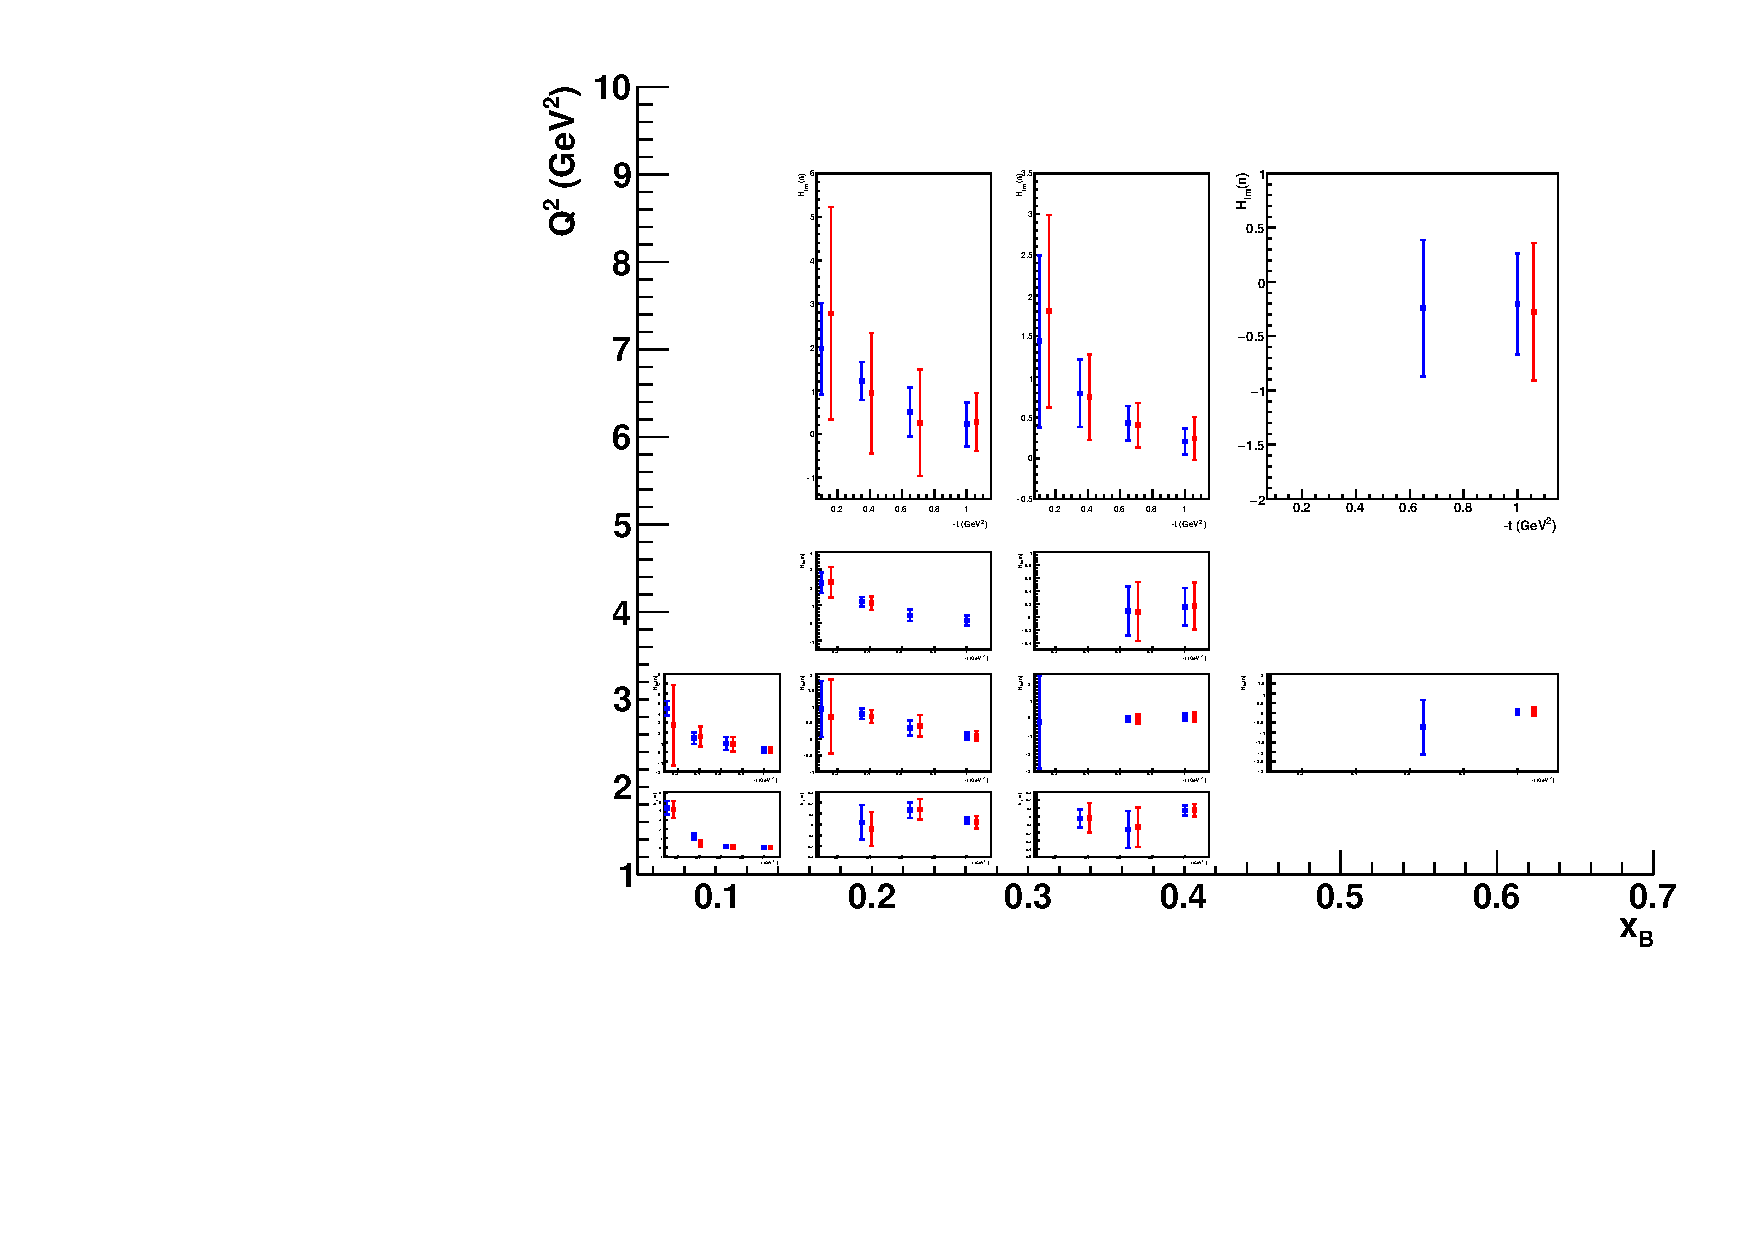
\includegraphics[width=200mm]{mixed_CFF/100/mixed/CFF_him_compare3.pdf}
\caption[$H_{Im}(n)$ as a function of $-t$]
{$H_{Im}(n)$ as a function of $-t$, for each bin in $Q^2$ and $x_B$. The blue points are obtained with the proposed run-group extension. The red points are obtained with the existing 50 days of Run Group Cb.}\label{cff_him}
\end{center}
\end{sidewaysfigure}

\begin{sidewaysfigure}  
\begin{center}
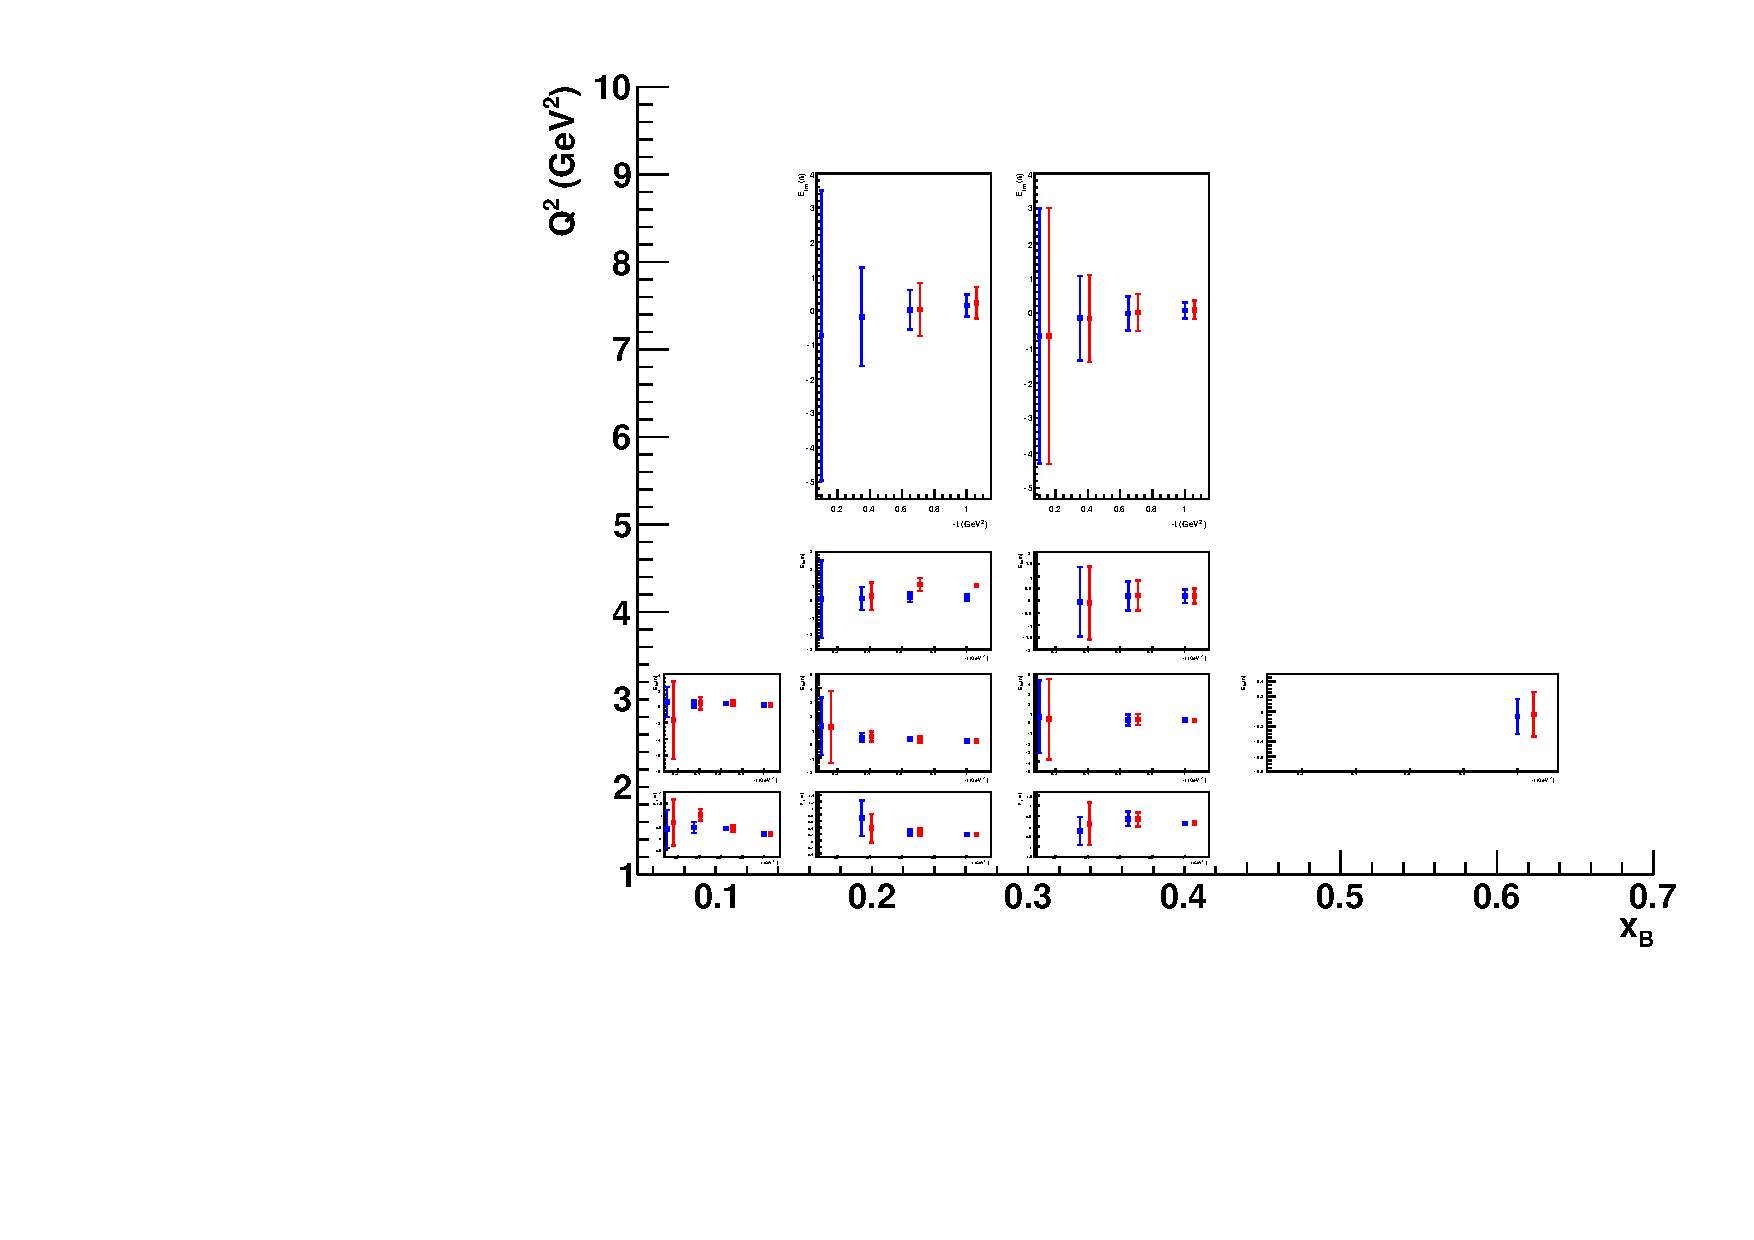
\includegraphics[width=200mm]{mixed_CFF/100/mixed/CFF_eim_compare3.pdf}
\caption[$E_{Im}(n)$ as a function of $-t$]
{$E_{Im}(n)$ as a function of $-t$, for each bin in $Q^2$ and $x_B$. The blue points are obtained with the proposed run-group extension. The red points are obtained with the existing 50 days of Run Group Cb.}\label{cff_eim}
\end{center}
\end{sidewaysfigure}

\begin{sidewaysfigure}  
\begin{center}
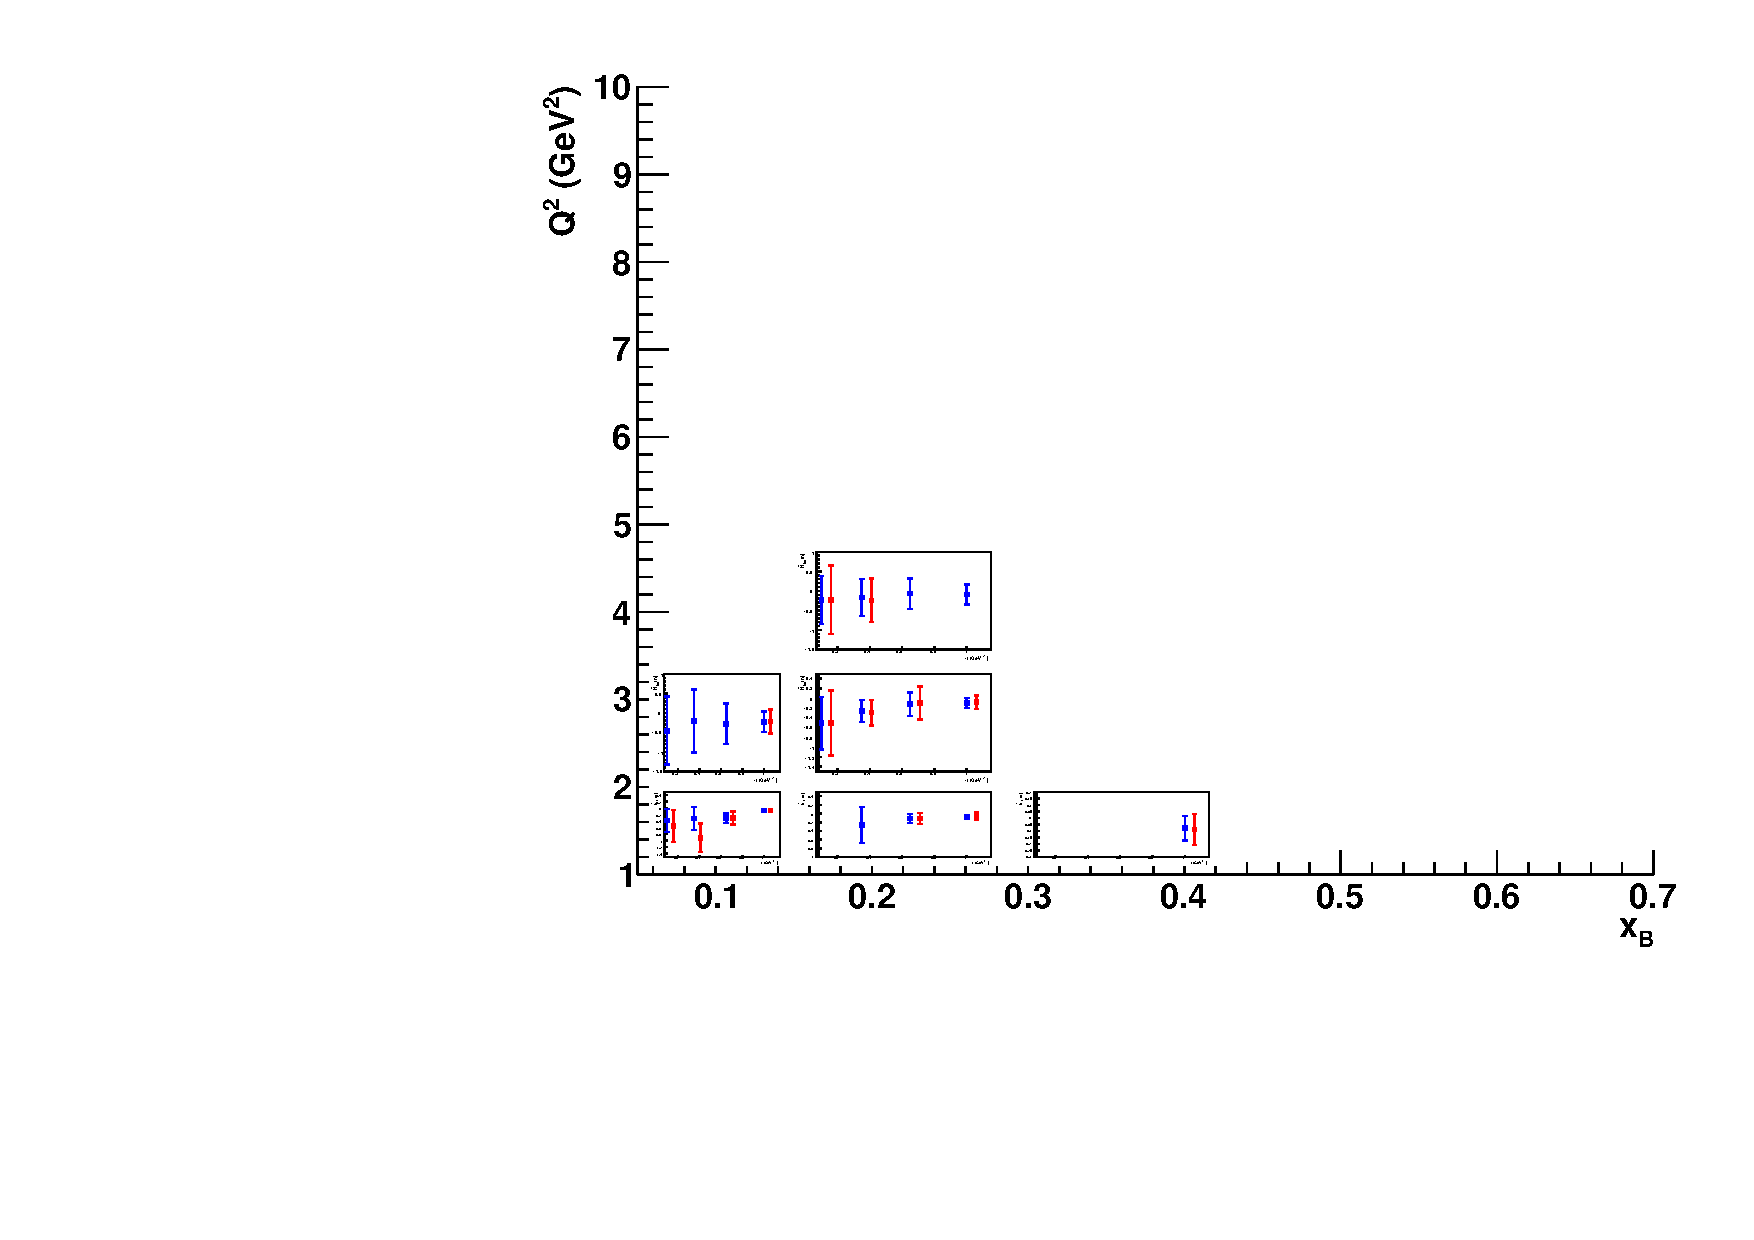
\includegraphics[width=200mm]{mixed_CFF/100/mixed/CFF_htim_compare3.pdf}
\caption[$\tilde{H}_{Im}(n)$ as a function of $-t$]
{$\tilde{H}_{Im}(n)$ as a function of $-t$, for each bin in $Q^2$ and $x_B$. The blue points are obtained with the proposed run-group extension. The red points are obtained with the existing 50 days of Run Group Cb.}\label{cff_htim}
\end{center}
\end{sidewaysfigure}

\begin{sidewaysfigure}  
\begin{center}
\includegraphics[width=200mm]{mixed_CFF/100/mixed/CFF_hre_compare3.pdf}
\caption[$H_{Re}(n)$ as a function of $-t$]
{$H_{Re}(n)$ as a function of $-t$, for each bin in $Q^2$ and $x_B$. The blue points are obtained with the proposed run-group extension. The red points are obtained with the existing 50 days of Run Group Cb.}\label{cff_hre}
\end{center}
\end{sidewaysfigure}

\begin{sidewaysfigure}  
\begin{center}
\includegraphics[width=200mm]{mixed_CFF/100/mixed/CFF_ere_compare3.pdf}
\caption[$E_{Re}(n)$ as a function of $-t$]
{$E_{Re}(n)$ as a function of $-t$, for each bin in $Q^2$ and $x_B$. The blue points are obtained with the proposed run-group extension. The red points are obtained with the existing 50 days of Run Group Cb.}\label{cff_ere}
\end{center}
\end{sidewaysfigure}

\begin{sidewaysfigure}  
\begin{center}
\includegraphics[width=200mm]{mixed_CFF/100/mixed/CFF_htre_compare3.pdf}
\caption[$\tilde{H}_{Re}(n)$ as a function of $-t$]
{$\tilde{H}_{Re}(n)$ as a function of $-t$, for each bin in $Q^2$ and $x_B$. The blue points are obtained with the proposed run-group extension. The red points are obtained with the existing 50 days of Run Group Cb.}\label{cff_htre}
\end{center}
\end{sidewaysfigure}

\begin{sidewaysfigure}  
\begin{center}
\includegraphics[width=200mm]{mixed_CFF/100/mixed/CFF_etre_compare3.pdf}
\caption[$\tilde{E}_{Re}(n)$ as a function of $-t$]
{$\tilde{E}_{Re}(n)$ as a function of $-t$, for each bin in $Q^2$ and $x_B$. The blue points are obtained with the proposed run-group extension. The red points are obtained with the existing 50 days of Run Group Cb.}\label{cff_etre}
\end{center}
\end{sidewaysfigure}

\section{Flavor separation of CFFs}
In order to convey the impact of the proposed measurement on the JLab GPD program, an example of model-independent flavor separation of CFFs, which this experiment will make possible for the first time, is shown in Figs.~\ref{flavor_h_im} and Figs.~\ref{flavor_e_im}. Here, the CFFs $H_{Im}$ (Fig.~\ref{flavor_h_im}) and $E_{Im}$ (Fig.~\ref{flavor_e_im}) are shown, for four different bins in $Q^2$-$x_B$ (left-right), as a function of $-t$, for the two nucleons (top) and for the two quark flavors (middle for $d$ and bottom for $u$). These figures has been produced using the proton CFFs that were extracted combining all the projected results for the pDVCS asymmetries that will be measured with CLAS12 \cite{mick_herve}\footnote{In the case of $E_{Im}$, the figure must be taken only as an indication of the potential of the present experiment. In fact the measurement of $E_{Im}(p)$, and its uncertainties, depend strongly on the feasibility of the conditionally approved pDVCS experiment with transversely-polarized target \cite{E1212010}.} (purple points), with the neutron CFFs that were shown in Section~\ref{sec_cff}, for the two different scenarios of beam time: the 110 days proposed in this extension request (blue points) and the existing 50 days of run group Cb (red points). 
Various observations can be made examining these figures: 
\begin{itemize}
\item{as noted before, $H_{Im}(n)$ is more sensible to variations of statistics for the ND$_3$ data than $E_{Im}(n)$, as the latter is mostly affected by the statistics of the beam-spin asymmetry; nevertheless, in some bins the impact of the extension will be important for $E_{Im}(n)$ as well. In particular, in some kinematics the fits for $E_{Im}(n)$ converge only thanks to the statistics provided by the extension;}
\item{in some kinematics, in particular at low $-t$ and low $x_B$, the presence of the Forward Tagger in the extension improves considerably the error bars or helps the fits to converge;}
\item{even with 110 days of running time on ND$_3$, the errors on neutron CFFs are much larger than those on proton ones, especially for $H$;}
\item{the uncertainty on neutron CFFs dominates the flavor-separated quark CFFs, impacting also the $u$ CFFs.}
\end{itemize}
The flavor separation of the CFFs will represent a major step forward towards the unraveling of the contribution of the quarks' angular momentum to the total nucleon spin via Ji's sum rule \cite{ji}: 
\begin{equation}
        \sum_{q}\int_{-1}^{+1}dx \, x[H^{q}(x,\xi,t=0)+E^{q}(x,\xi,t=0)]=2\, J_{quarks}.
        \label{eq_ji_rule}
\end{equation}
The low-$t$ region is very important for Ji's sum rule, and this motivates strongly the need to use the Forward Tagger to fill the gaps in the CLAS12 acceptance at such kinematics. 

\begin{figure}  
\begin{center}
\includegraphics[width=160mm]{flavors_h_im_compare3.pdf}
\caption[Flavor separation of the $H_{Im}$ CFF]
{Top: ${H}_{Im}(p)$ (purple), extracted from the projections for the approved and conditionally-approved proton-DVCS CLAS12 experiments, and ${H}_{Im}(n)$, obtained from the projections of the proposed experiment extension (blue) and from the projections for the already approved 50 days of run-group Cb (red), as a function of $-t$. The middle and bottom lines show the quark-flavor separated ${H}_{Im}$, for $d$ and for $u$ quarks, respectively. Four different bins in $Q^2$-$x_B$, indicated in the legends, are shown in the four columns.}\label{flavor_h_im}
\end{center}
\end{figure}

\begin{figure}  
\begin{center}
\includegraphics[width=160mm]{flavors_e_im_compare3.pdf}
\caption[Flavor separation of the $E_{Im}$ CFF]
{Top: ${E}_{Im}(p)$ (purple), extracted from the projections for the approved and conditionally-approved proton-DVCS CLAS12 experiments, and ${E}_{Im}(n)$, obtained from the projections of the proposed experiment extension (blue) and from the projections for the already approved 50 days of run-group Cb (red), as a function of $-t$. The middle and bottom lines show the quark-flavor separated ${E}_{Im}$, for $d$ and for $u$ quarks, respectively. Four different bins in $Q^2$-$x_B$, indicated in the legends, are shown in the four columns.}\label{flavor_e_im}
\end{center}
\end{figure}

\section{Systematic uncertainties}\label{sec_syst}
The goal of this experiment is to extract target and double-spin asymmetries, which are ratios of polarized cross sections. In the ratio, polarization-independent terms, such as acceptances, efficiencies, radiative corrections and luminosity, cancel out to a first approximation\footnote{Afanasev {\it et al.} \cite{afanasev} have computed the radiative corrections for the DVCS and BH processes on for CLAS kinematics. It was found that, given the strict kinematic cuts adopted to select the final state, the undetected radiated photon can only have small energies. In this case, therefore, the main contribution to the radiative correction comes from spin-independent soft-photon emission that does not affect the polarization observables. The approximation of negligible contribution from the radiative corrections to the BSA, TSA and DSA, compared to the size of the asymmetries, was estimated to be valid at the 0.1\% level \cite{afanasev}.}. Remaining effects could come from the quantities entering in the asymmetry definitions, namely the procedure to evaluate the counts $N^{+(-)}$, the dilution factor, the $\pi^0$ contamination, as well as the beam and target polarizations. 

Analyses performed at 6 GeV \cite{erin,pisano} showed that the biggest contributor to the overall systematic uncertainty is the selection of exclusivity cuts adopted to identify DVCS events and the corresponding counts $N^{+(-)}$. This factor contributed about 10\% (this and the following percentages for systematics are defined relatively to the average value of the TSA at $90^{\circ}$) to the total systematics uncertainty. 

Another source of uncertainty will be the $\pi^0$ background estimation, which will depend on the accuracy of the description of the detector acceptance and efficiency and on the model used in the Monte-Carlo simulation to describe the $en\pi^0(p)$ reaction (see Eq. 32). In order to account for this latter effect, 6-GeV analyses, performed on data taken on a polarized NH$_3$ target during the eg1-dvcs experiment \cite{erin,pisano}, evaluted this systematic by varying the contribution of the calculated background by $\pm 30\%$ (Section \ref{sec_pi0_back}), and extracting the final asymmetries in correspondence with this increased/decreased background. The total effect turned out to be 4\%, and a similar estimation can be assumed for the present experiment on ND$_3$.

While acceptance effects are expected to cancel in asymmetries, a residual effect could emerge due to the strong variations of the cross section inside the finite-size bins, that can lead, in principle, to a non-exact cancellation of acceptance effects from the numerator and the denominator. Such an acceptance effect has been estimated to bring an additional 1\% systematic error. 

To evaluate the systematic uncertainties linked to the dilution factor determination, in the aforementioned eg1-dvcs pDVCS analysis the  asymmetries were computed two more times, taking two different values of the dilution factor: $D_f+\Delta(D_f)$ and $D_f-\Delta(D_f)$, where $\Delta(D_f)$ is the statistical error that was estimated on this quantity. The resulting systematic uncertainties were found to be below the percent level. While studying the systematics on the exclusivity cuts, it was observed that changing the exclusivity cuts induces a variation of the dilution factors much bigger than the variations within the statistical errors described above. It was therefore decided, in order to avoid double-counting and therefore overestimation of systematics, to remove the contribution from the dilution factor computed according to its errors from the total systematic uncertainty. For this proposal, instead, a conservative estimate of the systematic uncertainty on the dilution factor of the order of 3\%, consistent with previous assumptions \cite{kuhn}, is assumed. 

%As for the systematic uncertainties on the dilution factors, in the aforementioned pDVCS 6-GeV analysis of eg1-dvcs were included in the exclusivity cut ones. Indeed, the systematic effect due to the variation of the exclusivity cuts represents the biggest contribution to the overall systematics, and, being the dilution factor strictly related to the specific set of exclusivity cuts adopted, its variation between the different sets of cuts turned out to be larger than its statistical error, making unnecessary a dedicated study.

An additional 2\% systematic effect is included in the total budget to account for the possible misidentification of neutrons due to accidental coincidences (Section~\ref{sec_accidentals}.)

Finally, uncertainties in the knowledge of the beam and target polarizations (extracted, respectively, via M{\o}ller polarimetry measurements and via the NMR system) will propagate into the asymmetry measurements, and are expected to lead to contributions of, respectively, 3\% and 4\%.

A summary of the systematic uncertainties can be found in Table~\ref{table_syst}. The total systematic uncertainty will be of the order of 12\%, averaged over all the kinematic bins (the $\pi^0$-background uncertainty will actually vary depending on the bin). 

\begin{table}
\begin{center}
\begin{tabular}{|c||c|}
\hline
Source of error & Systematic uncertainty\\
\hline
Channel selection cuts & 10\% \\
\hline
Beam and target polarization & 3\%-4\%  \\
\hline
$\pi^0$ contamination & 4\%  \\
\hline
Acceptance & 1\%  \\
\hline
Dilution factor & 3\%  \\
\hline
Accidentals & 2\%  \\
\hline
Radiative corrections & Negligible  \\
\hline
\hline
Total & 12\%  \\
\hline
\end{tabular}
\caption{Expected systematic uncertainties on the proposed measurement.}
\label{table_syst}
\end{center}
\end{table}

\section{Configuration change}
The change of configuration to insert the FT and change the shielding is estimated to take 4 calendar days \cite{miller_private}:
\begin{itemize}
\item{1 day to move the SVT/Solenoid/HTCC upstream to gain access to the shielding;}
\item{1 day to remove the M\o ller shield and the Forward Tagger tracker;}
\item{1 day to install the lead shield, M\o ller shield, outer shielding cone, and nose cone;}
\item{1 day to move the SVT / Solenoid / HTCC back into position.}
\end{itemize}
An additional two calendar days will be required to remove and reinstall the polarized target and recover its polarization. 
Considering that 1 calendar day is equal to 2 PAC days, in total the configuration change will require 3 PAC days. 


\section{Beam-time request}

We request 60 new PAC days of beam time for production running on the $^{14}$ND$_3$ target with an 11-GeV polarized electron beam, 50 of which at 10 nA of current with the same setup as run group Cb, and the other 10 at 5 nA with the addition of the Forward Tagger. 
These days will be added to the 50 already allocated for Run Group Cb. 
%This is necessary to obtain small enough error bars, for the two polarized-target observables, to allow us to bin them as finely as the BSA that will be extracted from the unpolarized-nDVCS experiment \cite{proposal}, and thus manage the CFF extraction by simultaneous fitting of the three observables.  
In order to acquire the roughly 10\% of counts on $^{12}$C that are necessary to estimate the dilution factor (Section~\ref{sec_dilution}) and to remove the nuclear background when studying the exclusivity cuts (Section \ref{sec_excl_cuts}), and given the maximum tolerable luminosity of CLAS12 of $10^{35}$ cm$^{-2}$s$^{-1}$, we will need a total of 10 PAC days of running on a 2-cm-long $^{12}$C target, also with a beam intensity of 10 nA. 
Eight days will be spent, with and without beam, in target-related operation, as explained in Section~\ref{sec_target_over}. 
Including 2 days of M\o ller runs to monitor the beam polarization (assuming a one-hour run per calendar day) the whole experiment, the part already approved plus the extension, and 3 days for the insertion of the Forward Tagger, the full experiment will take 133 days for completion. 

%We anticipate that approximately half of this request can be accumulated in parallel with other approved experiments utilizing the polarized ND$_3$ target (see Section~\ref{the_snake}).  We therefore request 50 new days of production running on ND3, combined with 12 days for ancillary measurements and overhead. 

\begin{table}
\begin{center}
\begin{tabular}{|c||c|}
%\hline
%Testing and commissioning & 2 days\\
\hline
Production data taking at $10^{35}$ cm$^{-2}$s$^{-1}$ on ND$_3$ & 100 days (50 are already approved)\\
\hline
Production data taking at $0.5 \cdot 10^{35}$ cm$^{-2}$s$^{-1}$ on ND$_3$ & 10 days (with FT)\\
\hline
Target work & 8 days\\
\hline
Production data taking on $^{12}$C target & 10 days\\
\hline 
M\o ller polarimeter runs & 2 days\\
\hline
Configuration change & 3 days \\
\hline
\hline
Total beam time request & 133 days\\
\hline
\end{tabular}
\caption{Total beam-time request, in PAC days, for the extension of Run-group Cb. This consists of 50 days already approved and the 60 additional days requested here, plus overhead.}
\label{beam_time}
\end{center}
\end{table}

%\section{Compatibility with other CLAS12 experiments/run groups}\label{the_snake}
%The collaboration recognizes that beam time during the 12 GeV era is a highly
%precious commodity, and that our request for 100+ days of this commodity must be
%well justified. As such, we reiterate that these first time measurements of
%target- and double-spin asymmetries in nDVCS, in tandem with the BSA measurements
%of E12-11-003, are absolutely necessary to make the first ever model-independent
%extractions of neutron Compton Form Factors, which will in turn allow first-ever flavor-separation of CFFs. The aforementioned experiment was granted 90 days from PAC38 and was later recognized as "High Impact" by PAC41. We respectfully suggest the present proposal has similar merit, and deserves the 100 days we request. Only in this way can the precision of its TSA and DSA results fully
%compliment the BSA measurements of E12-11-003, and permit a meaningful extraction of the neutron CFFs. 

%To make optimal use of the CEBAF12 beam, however, we anticipate that
%approximately half of our request can be accumulated in parallel with other
%approved experiments utilizing the polarized ND$_3$ target (E12-006-109,
%E12-007-107, and E12-09-007b) \cite{schedule}. We are therefore requesting 
%50 new days of production running on ND$_3$, combined with 12 days for ancillary 
%measurements and overhead.

\section{Conclusions}
Our knowledge of the three-dimensional structure of the nucleon has become richer in the last few years thanks to the introduction of the formalism of the Generalized Parton Distributions and to the subsequent wealth of experimental results on Deeply Virtual Compton Scattering which have recently become available. After the pioneering experimental results on DVCS, which raised the interest in this reaction as a means to achieve a tomographic description of the nucleon, it became evident, thanks to the analysis of the second generation of proton-DVCS dedicated experiments and to the advancement in the theory and phenomenology of GPDs, how only the combined measurement of several DVCS observables in a vast kinematic space can allow one to disentangle the contributions of the various GPDs and their complex kinematic dependences. While our knowledge of the three-dimensional structure of the proton is progressing considerably - the first attempts at its tomographic description have recently been made thanks to CLAS data taken at 6 GeV \cite{pisano,hs}, and a vast experimental program of pDVCS is planned for JLab at 12 GeV - neutron GPDs remain a mostly virgin field at this stage. The importance of extracing neutron CFFs is paramount if we want to ultimately perform a flavor decomposition of the GPDs. 
We propose here to make the first ever nDVCS measurements of spin observables, target- and double-spin asymmetries, with a polarized target.  We view the experiment as complementary to E12-11-003, which will measure the beam-spin asymmetries for nDVCS at the same kinematic points, and which is currently listed as a "high-impact" 12 GeV experiment. 
The detector system will include, for a subset of the data-taking time, the Forward Tagger, added to the standard CLAS12 configuration. This detector has been constructed, delivered to JLab and tested, and it is ready for installation. The polarized target is already being developed and will be used also for other CLAS12 experiments. The expected statistical precision and coverage for TSA and DSA that can be achieved with 100 days of beam time will allow us to extract, fitting them together with the BSA from E12-11-00, various neutron Compton Form Factors in a model-independent way. Quark-flavor separation will be obtained on various kinematic points by the linear combination of these neutron CFFs with the proton CFFs extracted from the pDVCS CLAS12 experiments. 

\newpage
\chapter{DIS on Longitudinally Polarized Deuterium}
\centerline{Proposal to increase the beam time allocation for the ND$_3$ part}
\centerline{of Experiment 12-06-109 (approved by PAC 30 and rated ``A'' by PAC 36)}
\vskip 0.4cm
\centerline{Sebastian Kuhn\footnote{contact person, email: skuhn@odu.edu}}
\centerline{\it  Old Dominion University, Norfolk VA 23529}

\abstract
{We are proposing to add 50 more days of running to the 50 days already approved for the portion of Experiment 12-06-109 with CLAS12 and 11 GeV polarized electrons on longitudinally polarized deuterons (ND$_3$). This additional beam time (plus overhead and carbon runs) will significantly reduce the uncertainty on polarized parton distributions, in particular for $d$ quarks, in the limit of large $x$, as well as for gluons and the strange quark sea at moderate to large $x$. It will bring the deuteron data at least closer to parity with the already approved 120 days of data on the proton, thus maximizing the information that can be extracted from a single experiment, as well as making more significant comparisons with other experiments (e.g. on $^3$He) possible. This will be important to assess the impact of nuclear effects on the extraction of $\Delta d$ at high $x$, and to guarantee that the unique opportunity to finally map out the asymptotic behavior of all quark distributions provided by Jefferson Lab's 12 GeV beam will be optimally utilized. In this proposal, we are providing updated estimates of various quantities that can be extracted from these data under the assumption of a doubling for the integrated luminosity on the deuteron.
}
\newpage
\setcounter{page}{72}
\section{Introduction}

Experiment 12-06-109 (together with E12-09-007b) is a comprehensive program to map out the $x$- and $Q^2$-dependence of the helicity structure of the nucleon in the region of moderate to very large $x$. By collecting inclusive (DIS) and semi-inclusive (SIDIS) data over a wide kinematic range with CLAS12 and 11 GeV polarized electrons on both longitudinally polarized protons (NH$_3$) and deuterons (ND$_3$), this program aims to constrain global fits of polarized parton (quark and gluon) distributions, extract higher twist corrections to the DIS structure functions, and evaluate moments connected to local operators in the Operator Product Expansion (OPE). 
Experiment 12-06-109 was originally approved by PAC 30 (with a further review and scientific rating of ``A'' by PAC 36) for a total of 80 days, 30 days on NH$_3$ and 50 days on ND$_3$ (both including overhead).

In the meantime, additional experiments~\cite{RGC} on longitudinally polarized {\em protons} have been approved, with high rating. These experiments have brought the total number of PAC-approved days for the NH$_3$ target to 120 (run group Ca with CLAS12). 
In the meantime, the total runtime for the ND$_3$ target (run group Cb) has been largely unchanged (at present 65 days including all overhead for auxiliary measurements, target operations etc.). This discrepancy is even more striking when taking into account that ND$_3$ targets tend to have polarizations of roughly a factor 1/2 lower than NH$_3$ targets, resulting in an overall figure of merit (FoM) at least four times worse than for the proton. This means that any  analysis that requires information from both targets (e.g., global fits to extract polarized parton distributions) would have uncertainties that are totally dominated by the statistical error from the deuteron.

While some of the goals of the original experiment 12-06-109 can be reached with reasonable precision even with 50 PAC days on the deuteron, there are some physics observables whose precision would be ``statistics-starved'' under this scenario. In particular, the asymptotic behavior of the PDF $\Delta d$ at large $x$ would be much less constrained than what is possible with a doubling of the integrated luminosity. Deuteron data are also crucial to determine the total contribution from quark helicities to the nucleon spin ($\Delta \Sigma$), as well as polarized gluon and strange quark PDFs at moderate to large $x$ (see details in the following sections). Because of their smaller count rates, SIDIS channels will benefit significantly from additional statistics. As we lay out in detail in the following sections, a doubling of the actual run time on polarized ND$_3$ from 50 to 100 days (plus the necessary overhead) will optimize the overall physics output from Experiment 12-06-109 and maximize the return on the large investment in the spin physics program with Jefferson Lab at 12 GeV.
No other facility presently running or under construction will be able to probe, with comparable precision, the kinematic region of moderate to large $x$ and moderate $Q^2$ accessible here.

%The additional 10 days at 5 nA with the inclusion of the Forward Tagger, as requested in the nDVCS part of this proposal, will not directly impact the program of measuring collinear spin structure functions, and has not been included in the estimates that follow in this chapter. However, it offers the potential for measurements of spin structure functions at very low $Q^2$ (measuring the scattered electron in the FT), that are of interest in their own right, and as part of the radiative corrections for DIS. 

%To fully elucidate the spin structure of the nucleon in the valence region, one has to combine 
%information from many different experimental approaches. Both deeply virtual exclusive processes,
%which are sensitive to Generalized Parton Distributions (GPDs), and semi-inclusive processes (in particular
%those involving single spin asymmetries which are sensitive to Transverse Momentum-dependent Distributions - TMDs)
% will access some part of this puzzle. However, high precision
%measurements of structure functions (as well as of elastic form factors) remain indispensable, both to
%constrain the parameters of GPD and TMD fits, and as the most direct access to the longitudinal structure
%of the nucleon. In particular, spin structure functions of the nucleon in the valence region and at very large
%$x$ are still poorly known, in spite of their fundamental significance for tests of pQCD and models of
%nucleon structure. Jefferson Lab with 11-12 GeV beams is the unique place where this gap can be finally closed.
%The accessible kinematics is also uniquely suited to study the transition from partonic degrees of freedom
%to hadronic ones, through detailed measurements of higher twist operator matrix elements and a
%complete investigation of the phenomenon of quark-hadron duality in spin structure functions.

\subsection{The Deuteron and CLAS12}

A complete mapping of spin structure functions and the extraction, through global PDF fits, of polarized parton distributions require a complete set of measurements on both types of nucleons, protons and neutrons, over the widest possible range in $x$ and $Q^2$. 
In addition, since neutrons can only be accessed bound in nuclei, it is very important that both commonly used nuclear targets, $^3$He and deuterium, be studied with high precision, since nuclear effects and their uncertainties are very different for these two cases. Furthermore, the deuteron is the best substitute for a purely isoscalar nucleon target, which is ideal for extracting information on gluon and sea quark helicity distributions through NLO analyses. For these reasons, a high-statistics measurement on polarized deuterium (ND$_3$) is obligatory.

Presently, the only readily available and suitable targets for polarized protons and deuterons employ solid state compounds like ammonia, butanol or lithium deuteride at low ($\approx 1$ K) temperatures. 
These compounds are susceptible to radiation damage and beam heating, limiting severely the practically achievable luminosities. 
The upgraded CLAS12 detector will be a perfect match for these targets, since it
\begin{itemize}
\item is optimized for luminosities of 1-2$\cdot 10^{35}$ cm$^{-2}$ s$^{-1}$, within a factor of 2-4 of the practical limit of cryogenic ammonia targets, and compensates for this relatively low luminosity with its very large acceptance
\item already contains a solenoidal magnet which will provide the (typically 5 Tesla) field needed for dynamic nuclear polarization, thus minimizing the extra costs of a polarized target
\item covers a large angular range, including backwards angles, which allows us to simultaneously measure inclusive, semi-inclusive and tagged structure functions (with backward-going target remnants) over the full kinematic range of interest (while also collecting data for deeply virtual exclusive processes and single spin asymmetries).
\end{itemize}

Our group is leading the development of an optimized longitudinally polarized proton and deuteron target for CLAS12, and coordinates the run group C using these targets. Significant investments in this program have already been made, partially through an NSF MRI grant. No other experiment with this particular type of targets has been planned with similar kinematics, at Jefferson Lab or elsewhere. We believe that adding 50 more days of running, plus overhead, to the already established run group C (an overall increase by only 25\%) will yield an optimal return on this investment.

\section{Scientific Case and Recent Developments}

\begin{figure}[htb!]
\begin{center}
\includegraphics[width=6in]{dis/LT_all_groups.pdf}
\end{center}
\caption{\baselineskip 13pt \small
Compilation of recent  polarized PDF fits from various groups. This Figure is from the  JAM15 paper~\cite{JAM15}
(Fig. 17) where all references for these fits can be found.}
\label{NLOfits}
\end{figure}

Inclusive and flavor-tagged spin structure functions of the nucleon have been measured for  over three decades~\cite{Kuhn:2008sy}, beginning with the
experiments at SLAC~\cite{Alguard:1976bm} and the discovery of the famous ``spin puzzle'' by the 
EMC~\cite{EMCfinal}. The goal of these experiments is to determine, via next-to-leading-order DGLAP analyses, 
 the helicity-dependent distribution functions (PDFs)
 of valence and sea quarks as well as gluons, see Fig.~\ref{NLOfits}. Collinear spin structure functions can also be used to evaluate 
 moments that are related to nucleon axial current matrix elements (e.g., the overall contribution of quark helicities to the
 nucleon spin), and to test fundamental sum rules like the Bj\"orken sum rule~\cite{Bjorken:1968dy}. 
 Finally, measuring their dependence on the
 photon virtuality $Q^2$ allows us to determine higher twist contributions, matrix elements in the framework of the operator
 product expansion (OPE), and the transition from partonic (high $Q^2$) to hadronic (low $Q^2$) degrees of freedom,
 including duality and 
 tests of the Gerasimov-Drell-Hearn sum rule and its extensions in, e.g., Chiral perturbation theory (see
 discussion and references in~\cite{Kuhn:2008sy}).
 In the new era of three-dimensional mapping of the nucleon parton distributions, collinear spin structure functions
 serve both as a crucial constraint on GPDs and TMDs, and provide two of the four ingredients to the celebrated
 nucleon spin sum rule.
 
Within recent years, data from high-energy polarized proton collisions at 
RHIC~\cite{STAR_jet15,PHENIX_pi14,PHENIX_pi15,STAR_W14,PHENIX_W15} 
have constrained the contribution of gluon
and sea quark helicities at low to moderate $x \le 0.2$ to the nucleon spin. Further information has come from measurements
of open charm production~\cite{COMPASS_g13}. The most recent 
inclusive data from COMPASS~\cite{COMPASS16} extend our knowledge of spin structure functions to the lowest
$x$ and highest $Q^2$ yet. 
Meanwhile, the spin structure function program with Jefferson Lab's 6 GeV has been concluded and most results have been 
published. In particular, very precise data on proton, deuteron and $^3$He 
targets~\cite{eg1b-d,eg1b-p,eg1-dvcs,E06-014_A1,E06-014_d2,E01-012}
 have recently appeared 
that cover a large kinematic range, from low $Q^2$ to the DIS region. This program is being continued in the 12 GeV era, with several
experiments in three halls approved with scientific rating of ``A''. The unique importance of these expected Jefferson Lab 
data is threefold:

\begin{figure}[htb!]
\begin{center}
\includegraphics[width=6in]{dis/IMPACT_JLAB.pdf}
\end{center}
\caption{\baselineskip 13pt \small
Impact of recent Jefferson Lab data on the global NLO PDF fit by the Jefferson Lab Angular Momentum (JAM) collaboration. 
This Figure is from the recent JAM15 paper~\cite{JAM15}
(Fig. 15) where all relevant references  can be found. The l.h.s. fits are for the leading twist distributions for three quark flavors
and gluons, while the r.h.s. shows the results for various higher-twist terms.The yellow lines are from repeated
Monte Carlo fits including all world data except those from Jefferson Lab; the red lines include the Jefferson Lab data and
clearly have a much more narrow uncertainty band.}
\label{JLabImpact}
\end{figure}

\begin{enumerate}
\item For a DGLAP determination of all individual parton distribution functions, but in particular those of the gluon, from DIS data,
a large leverarm in $Q^2$ is required to exploit scaling violations. The recent precise data from COMPASS~\cite{COMPASS16}
cover the high-$Q^2$ limit\footnote{These will be greatly improved upon, both in kinematic reach and in precision, by data
to be acquired with the future EIC; however, the low-$Q^2$ data fromJefferson Lab will likely not be matched in the foreseeable future.},
 while precise data at the lowest $Q^2$ consistent with DIS come from Jefferson Lab. The latter cover 
a large range in $Q^2$, which in itself allows us to reliably extract and control for higher-twist effects. Figure~\ref{JLabImpact}
demonstrates the significant improvement in our knowledge of {\em all} polarized PDFs enabled already by the existing
Jefferson Lab data.

\begin{figure}[htb!]
\begin{center}
\includegraphics[width=4in]{dis/delqFig-eps-converted-to.pdf}
\end{center}
\vspace{-0.2in}
\caption{\baselineskip 13pt \small
$\Delta u/u$ (upper half) and $\Delta d/d$ (lower half) results from Jefferson Lab
Hall A and CLAS data (in leading order approximation), compared with other world data
and three different predictions: a fit by Leader, Stamenov and Siderov~\cite{Leader:2006xc} (black line), and two pQCD
predictions without~\cite{Brodsky:1994kg} (dashed)  and with~\cite{Avakian:2007xa} (solid red and blue lines)
inclusion of orbital angular momentum effects.  }
\label{highx}
\end{figure}

\item While the contribution from PDFs in the valence region $x > 0.3$ and, especially, in the limit $x \rightarrow 1$, to the overall
nucleon spin is not very large, knowledge of PDFs in this regime is crucial to understand the valence structure of the nucleon and to
test predictions from pQCD and various models. Only Jefferson Lab at 12 GeV can provide the necessary precision data
in these kinematics for the foreseeable future. In particular, the asymptotic polarization of d quarks in the proton,
$\Delta d/ d$ at large $x$, is presently poorly known (see Fig.~\ref{highx}), 
and a reliable measurement requires high statistics data from both
deuterons and $^3$He.

\item Beyond the leading-order PDFs, higher twist structure functions are of high current interest in themselves, since
they contain information about correlations and interactions between gluons and quarks in the nucleon. Again, only at Jefferson Lab, with its unique combination of high luminosity
and moderate $Q^2$, can these structure functions be studied in detail (see
the r.h.s. of  Fig.~\ref{JLabImpact} for
examples).
\end{enumerate}

\begin{figure}[hbt!]
\begin{center}
\includegraphics[width=2.5in]{dis/Coverage2-eps-converted-to.pdf}
\end{center}
\caption{\baselineskip 13pt \small
Kinematic coverage in the DIS region
 of existing 6 GeV JLab experiments and expected coverage
for the proposed 12 GeV experiment.}
\label{coverage}
\end{figure}

Experiment 12-06-109 at 11 GeV will 
 extend the useful $x$-range in the DIS region both to lower and
higher $x$ and to much higher $Q^2$, compared to the existing Jefferson Lab data; see Fig.~\ref{coverage}.
Especially at the upper end, the expected data will still be limited in statistics; a doubling of the
integrated luminosity will yield significant improvements in the information we can extract from these data,
as we will show below.

%\section{Technical Progress Towards Realizing the Experiment}
%The proposed experiment will use the standard equipment of CLAS12 in addition to the
%polarized target. Many of the authors on this proposal are actively working on several of the
%detector components of CLAS12, including pre-shower calorimeter, high threshold cherenkov 
%counter,  and Region 1 and 2 forward tracking drift chambers, as well as data analysis software. 
%All of these projects have made significant progress since the experiment was originally approved;
%for example, the first Region 2 drift chamber has been assembled and stringing has begun
%at JLab, with subsequent sectors to be strung in ODU's newly completed clean room.
%
%\begin{figure}[ht]
%%\vspace{-0.2in}
%%\includegraphics[width=12cm, angle=90]{ConceptCutaway1.eps}
%%\vspace{-1in}
%\begin{center}
%\includegraphics[width=6in]{Target.eps}
%\end{center}
%%\centerline{\epsfxsize=6in\epsffile{Target.eps}}
%\caption{\baselineskip 13pt \small
%A schematic drawing of the polarized solid target cryostat and 
%target insert for CLAS12. Note that the required 5 Tesla polarizing magnetic field
%will be provided ``for free'' by the solenoid of the CLAS12 central tracker, which
%was designed with this goal in mind. The target sits inside a horizontal $^4$He
%evaporation refrigerator and will be dynamically polarized using a microwave system. \label {potarg}}
%\end{figure}
%
%The major non-standard item required for successful execution of this program is the polarized target.
%A conceptual design was already completed at the time of the first PAC submission, see Fig.~\ref{potarg}.
%Unfortunately, funding for this target had been 
%subsequently removed from the base equipment budget for the 
%Jefferson Lab 12 GeV upgrade, to cover required contingency costs in other parts of the project.
%In 2009, some of the spokespersons of this experiment (Kuhn, B\"ultmann, Prok, and Crabb) formed
%a consortium and submitted a successful MRI-R$^2$ proposal to NSF. The approved funding from
%this source will cover all costs of acquiring necessary hardware and prototyping, assembly,
%and testing of the polarized target. Subsequent to the availability of these funds, work has begun on
%the detailed design of all target components, in particular the in-beam cryostat and vacuum vessel.
%The design of the central Silicon Vertex Tracker for CLAS12 is now fully consistent with the required
%space to insert the polarized target into its center.
%Initial development work has also begun on the target insert and NMR system; several major components
%and measuring instruments have already been acquired. The total project, which also receives strong
%support from the JLab target group, is on track to be completed within 4 years, making the polarized
%target available as soon as the experimental program with CLAS12 can begin. In addition to the present
%experiment, this target also supports a large (PAC-approved) program of measurements of 
%DVCS (E12-06-119), SIDIS (single target spin asymmetries;  E12-07-107),
% and of the EMC effect in nuclear spin structure functions (LOI 10-005 to PAC35).
%
%At PAC34, a series of SIDIS experiments (Proposals PR12-09-007, 008, 009) were approved for both
%unpolarized and longitudinally polarized target. All of these proposal require a RICH detector (in lieu
%of some sectors of the existing low-threshold cherenkov counter) to separate Kaons from pions
%and protons. Work on the design of such a RICH detector has begun in earnest, and first 
%benchmark results have been presented at CLAS12 workshops. This development will clearly
%benefit the present experiment, as well, as it will allow us to access the full kinematic range of
%flavor-tagged spin structure functions in SIDIS, with separation of all three charge states of pions
%and kaons. This will lead to additional constraints of NLO analyses which will allow us to separate the
%contributions of valence and various sea quarks in the range $x > 0.1$, where existing data
%have relatively large uncertainties and one expects interesting effects to appear (e.g.,
%a possible charge asymmetry in the polarized sea, analog to that seen in unpolarized PDFs).
%Several of the authors of this proposal update are working on this extension of the CLAS12 
%capabilities.

\section{Expected Results}

\subsection{PDFs}

\begin{figure} [!htbp]
\includegraphics[width=\linewidth]{dis/LTrat.pdf}
\caption{\baselineskip 13pt \small
Expected effect on the uncertainty for various polarized parton distribution
functions after inclusion of E12-06-109 data, according to an up-to-date
analysis by the JAM collaboration (courtesy of N. Sato). 
The blue lines indicate the reduction factor for the present uncertainties (see Fig.~\ref{JLabImpact}) 
from the already approved 120 days of NH$_3$ only, while the green and red lines show the additional reduction from
combining these data with either the already approved 50 days for ND$_3$ (green), or with double that run time (red).}
%PLACEHOLDER: TO BE REPLACED BY UP-TO-DATE JAM RESULTS:
%Expected uncertainties for polarized parton distributions
%$\Delta u$, $\Delta d$, $\Delta G$ and $\Delta s$
%from a NLO analysis of all world data. The two outermost lines show the
%result  by Leader, Sidorov and Stamenov~\protect{\cite{Leader:2006xc}}
%discussed above. The innermost line shows the expected uncertainty after including
%the data set to be collected with this experiment, including statistical and systematic errors.
%Note that the $x$-range where these data will have the most impact depend on the
% functional form of the PDF parametrizations; nevertheless, the much smaller errors
% shown here are indicative of the statistical power in that $x$-range. }
\label{pPDFs_exp}
\end{figure}

The main goal of E12-06-109 is to determine the $x-$dependence of each individual parton (quark {\em or} gluon) distribution
in the region of moderate to very high $x$, $0.06 \le x \le 0.8$. This is the region most relevant to the low-energy properties of the
nucleon, where valence quarks and sea quarks confined in the ``meson cloud'' dominate. It is also the region where 
measurements at RHIC and charm production at COMPASS can contribute only little but which is important
to our understanding of the dynamics that impart a net 
polarization to the ``valence-like'' sea quarks and gluons at high $x$. 

Figure~\ref{pPDFs_exp} shows the expected improvement for the
uncertainties on up, down, and strange quark polarizations as well as the gluon 
polarization from E12-06-109. The blue lines show the improvement due to just the proton data 
from the presently allocated beam time (120 days on NH$_3$), while the green lines show the further reduction
in those uncertainties due to the expected deuteron data as approved (50 days on ND$_3$).
Finally, the red lines show how the impact of collected twice the statistics on the deuteron, as proposed here.
It is clear that the biggest improvement from the deuteron data will be in our knowledge of the down quark polarization
(see bottom left panel of Fig.~\ref{pPDFs_exp}). This is also the case where doubling the beam time has the largest
impact, reducing the uncertainty on $\delta d$ by roughly a factor 3/4 in the moderate to high $x$ region. However, as
Fig.~\ref{pPDFs_exp} shows, nearly all polarized PDFs will benefit from the additional beam time requested here.

It is important to clarify that the total uncertainty on the deuterium data points is largely driven by accumulated
statistics. The most important systematic uncertainty will be the normalization of the data due to the product of beam
and target polarization and due to the dilution factor. Both of these quantities will be determined 
experimentally (directly - for the polarization -
or indirectly through auxiliary measurements). In particular, the polarization product $P_b P_t$ will be extracted from a measurement of the exclusive
D$(e,e^\prime p)n$ reaction, for which the expected double-spin asymmetry is very well known and sophisticated models for final
state interactions exist (which our group has tested experimentally~\cite{Mayer}). Due to the somewhat small magnitude of this asymmetry
(driven by the requirement of low $Q^2$ to get reasonable count rates), this measurement requires high statistics. Data will be
taken simultaneously with DIS and other channels, meaning that the the uncertainty in $P_b P_t$ will decrease proportional to that
in the measured structure functions. Similarly, the dilution factor will be determined using sophisticated models of electron 
scattering from the various nuclear components of the target; however, some normalization factors (e.g., overall target density
of the various species) have to be taken from precise measurements on auxiliary targets. These measurements will gain
the same improvement in statistics as the main measurements on ND$_3$.


\subsection{Quark polarization at high $x$}

\begin{figure}[htb!]
\begin{center}
\includegraphics[width=\linewidth]{dis/NewHighX.pdf}
\end{center}
\caption{\baselineskip 13pt \small
Expected statistical precision for the polarization of d quarks, $\Delta d / d$, versus $x$, extracted from E12-06-109 as approved
(l.h.s.) and with an additional 50 days of beam time on the deuteron (r.h.s.). Existing data are shown lightly shaded
(squares are from CLAS at 6 GeV) while the expected data are shown as blue diamonds. The two curves are
the expectations from pQCD without~\cite{Brodsky:1994kg}  and with~\cite{Avakian:2007xa} inclusion of orbital angular momentum effects. The expected data are placed according to expectations from hyperfine-perturbed quark models~\cite{Isgur:1998yb} which,
at least at present, cannot be ruled out.}
\label{highXexp}
\end{figure}

In Figure~\ref{highXexp}, we focus on the impact our proposed data will have on the determination of the d-quark polarization
at the highest $x$ reachable with Jefferson Lab at 12 GeV. The ``expected data points'' are based on a detailed Monte Carlo simulation
of the measured asymmetries on the proton and the deuteron, including both statistical and systematic uncertainties.
While we used a simple-minded LO (``na\"ive parton model'') calculation to extract the valence quark polarizations from these
measurements, the expected uncertainty will not change much with a more sophisticated analysis like the JAM PDF fit 
described above. The obvious point from this figure is that, as presently scheduled, our expected data will have limited
statistical power to definitely answer the question (by themselves) whether $\Delta d / d$ remains negative for $x \rightarrow 1$
as expected from some NLO fits~\cite{Leader:2006xc} and from hyperfine-perturbed quark models~\cite{Isgur:1998yb} or whether it 
will converge to $+1$ as expected by pQCD, as indicated in the solid curves in Fig.~\ref{highXexp}. In particular, the two last
data points are only 3.7 and 1.2 standard deviations from zero, so with a statistical fluctuation of the actually measured data points 
by only one standard deviation, the solid curve in Fig.~\ref{highXexp} would still be (nearly) compatible with those data,
with a $\chi^2$ of 4.9 for two degrees of freedom ($p = 8.7 \%$). 

With a doubling of the integrated luminosity on the deuteron, the statistical error bars on $\Delta d / d$ will go down nearly exactly
by a factor of $1/\sqrt{2}$, since the proton results (that also enter the calculation) are already vastly more precise than the deuteron
ones. As stated above, the systematic uncertainties will also go down, by nearly the same amount (and the uncertainties
 are statistics-dominated
at high $x$). Repeating the same calculation, we find that the agreement with the ``wrong'' curve is now much worse, with
a $\chi^2$ of 11.3 for two degrees of freedom ($p = 0.35 \%$). While it is true that more information on $\Delta d / d$ is expected
from the approved experiments on $^3$He, it is precisely at high $x$ that smearing effects and uncertainties from nuclear binding
become the largest, making an independent measurement on the most lightly bound nucleus, deuterium, mandatory. Our
proposal for an additional 50 days on that target will strengthen this independent result significantly.

\subsection{Further results from SIDIS}

%We request 25 days of highly polarized ($> 85 \%$) electron beam (about 10-20 nA) on a 3 cm long
%NH$_3$ target (80 \% polarization on average) and 45 days on a 3 cm long ND$_3$ target 
%(40 \% polarization on average). In addition, we request 10 days of beam on auxiliary targets
%(carbon - 8 days, and empty - 2 days). We also will need 5 additional days (without beam) for
%target changes, anneals
%(which will be needed about every other day), polarization reversals, and calibrations. The quoted
% parameters are fully consistent with recent operating experience
%during eg1-DVCS, which ran in 2009, including several days on an ND$_3$ target (which exhibited
%a slow drop of its polarization from about 43\% to 33\% during a 2-day period after it received its
%optimal radiation dose). The beam time requests are optimized so that statistical errors will be 
%smaller or comparable to systematic ones in all kinematics of interest. In particular, the running
%time on deuterium is longer to partially compensate for the lower polarization and to
%maximize the impact on NLO extractions of polarized parton densities. In Figs.~\ref{A1eg12}-\ref{rest} 
%we show a few 
%representative results expected from this data set; these as well as additional plots (based on
%a full simulation of CLAS12) are contained in the original proposal.


\begin{figure}[htb!]
\includegraphics[width=0.66\linewidth]{dis/DeltaDoverD-eps-converted-to.pdf}
%\end{minipage}%\hfill
\caption{\baselineskip 13pt \small
Expected results for the valence $d$ quark polarization from semi-inclusive data
with the proposed experiment, as well
as existing data. The horizontal risers indicate the systematic uncertainties, while the length of the error bars
indicates the statistical uncertainties.
The dashed line represents a pQCD prediction~\cite{Brodsky:1994kg}
 while the solid line represents the prediction from the
  hyperfine perturbed constituent quark model~\cite{Isgur:1998yb}. }
\label{rest}
\end{figure}

In addition to the determination of polarized PDFs from inclusive DIS measurements,  run group C also supports a large number
of approved measurements with semi-inclusive detection of pions and Kaons. For example, we show in Fig.~\ref{rest} the
expected results from a combination of SIDIS production of pions ($\pi^+$ and $\pi^-$) from both proton and deuteron targets
that directly measures (in LO) the valence d-quark polarization. This figure is from the original proposal for E12-06-109
and hasn't been updated yet, but it is clear that similar arguments as for the previous subsection apply: A reduction of the 
statistical error bars (indicated by the {\em full} length of the vertical lines) by a factor $1/\sqrt{2}$ would turn this marginally
significant measurement into a strong, independent confirmation for the trend observed in DIS.

\begin{figure} [!htbp]
\begin{minipage}[t]{0.5\linewidth}
%\epsfxsize=\linewidth
\includegraphics[width=\linewidth]{dis/Kplusd.pdf}
\end{minipage}%\hfill
\begin{minipage}[t]{0.5\linewidth}
%\epsfxsize=\linewidth
\includegraphics[width=\linewidth]{dis/Kminusp.pdf}
\end{minipage}
\begin{minipage}[b]{\linewidth}
%\epsfxsize=\linewidth
\includegraphics[width=\linewidth]{dis/Kminusd.pdf}
\end{minipage}%\hfill
\caption{\baselineskip 13pt \small
Contributions to the measured asymmetry in SIDIS Kaon production from various quark (solid lines) and
anti-quark (dashed lines) flavors, according to a preliminary JAM
analysis. The data points are from HERMES.
The top row shows  the $K^+$ asymmetry on the deuteron (l.h.s.) and the $K^-$ asymmetry on the proton
(r.h.s.). The bottom row shows two fits to the $K^-$ asymmetry on the deuteron, either with the s-quark contribution
allowed to vary freely for a minimized $\chi^2$ (left) or with this contribution set to zero (right). Figure courtesy of J.J. Ethier. }
\label{kaon}
\end{figure}

More generally, a combined analysis of all inclusive and semi-inclusive measurements within the framework of NLO DGLAP
analysis will further constrain the individual quark and gluon PDFs and allow a clear separation of quark and antiquark
contributions of each flavor to the sea. The JAM collaboration is now gearing up to include this information in their fits,
carefully assessing the impact of our (lack of) knowledge of the required fragmentation functions. While simulations are not
yet available, it is clear again that higher precision will translate in additional knowledge. As an example we consider
(in Fig.~\ref{kaon}) the impact of various measurements on our knowledge of the strange quark sea in the nucleon, which
is still a contentious topic without a clear consensus whether the contribution of this strange sea to the nucleon spin is
positive, negative or negligible.

The top row of Fig.~\ref{kaon} shows that the $K^+$ asymmetry (on either target) and the $K^-$ asymmetry on the proton are rather insensitive
to the strange quark polarization, since in both cases u-quarks dominate because of their prevalence and larger charge.
However, the $K^-$ asymmetry on the deuteron is much more sensitive to strange quarks, since in the deuteron,
u and d quark contributions to $K^-$  production fortuitously cancel to a large extent. Hence, a precise measurement of
this channel down to the lowest available $x \approx 0.06$ at Jefferson Lab has great promise to answer the question whether
strange quarks in the nucleon carry positive helicity, negative helicity or whether there is a node in the distribution where
their polarization transitions from plus to minus.
Unfortunately, the only data existing so far (from HERMES) have large error bars, so that an alternative fit without any
s-quark contribution only increases the $\chi^2$ per degree of freedom from 0.38 to 0.51 (see bottom row of Fig.~\ref{kaon}).
With the vastly better statistics available from CLAS12, this situation should be much improved (note that CLAS12
will cover the same kinematic region as HERMES except for the two lowest data points). The importance of
finally ``nailing down'' this least-known quark contribution to the nucleon spin is another strong justification to collect
the highest statistics data set on the deuteron possible.

\section{Beam Request}

We request 50 additional days, for a total of 100 days, of 11 GeV longitudinally polarized ($> 85 \%$) electrons on a longitudinally polarized ND$_3$ target in CLAS12, plus 23 additional days for calibration, in-situ irradiation of the target material, target changes, anneals and polarization reversals, as well as beam polarization (M\o ller) measurements. 
The additional 10 days at 5 nA with the inclusion of the FT, as requested in the nDVCS part of this proposal, will not directly impact the program of measuring collinear spin structure functions and has not been included in the estimates that were presented in this chapter. However, it offers the potential for measurements of spin structure functions at very low $Q^2$ that are of interest in their own right, and as part of the radiative corrections for DIS.

\newpage
\chapter{Semi-Inclusive Deep Inelastic Scattering on a longitudinally polarized deuterium target}
\centerline{Proposal to increase the beam time allocation for the ND$_3$ part}
\centerline{of Experiments E12-07-107 and E12-09-009}
\vskip 0.4cm
\centerline{S. Pisano\footnote{contact person, email: pisanos@jlab.org}}
\centerline{\it INFN, Laboratori Nazionali di Frascati, 00044 Frascati, Italy}
%\vskip 0.4cm
%\centerline{S. Niccolai\footnotemark[1]}
%\centerline{\it Institut de Physique Nucl\'eaire d'Orsay, 91406 Orsay, France}
%\vskip 0.4cm
%\centerline{A. Biselli\footnotemark[1]}
%\centerline{\it Fairfield University, Fairfield Connecticut 06824}
%\vskip 0.4cm
%\centerline{C. Keith\footnotemark[1]}
%\centerline{\it Thomas Jefferson National Laboratory, Newport News, VA 23606}
%\vskip 0.4cm
%\centerline{D. Sokhan\footnotemark[1]}
%\centerline{\it University of Glasgow}
%\vskip 0.4cm

\abstract{A comprehensive program to study Transverse Momentum Dependent distribution functions is foreseen for CLAS12. In particular, the E12-07-107 and E12-09-009 experiments aim to access the valence-quark transverse and longitudinal spin distributions through measurements of spin-azimuthal asymmetries in semi-inclusive electroproduction of pions and kaons. They will make use of the upgraded JLab 11-GeV polarized electron beam and the CLAS12 detector with longitudinally polarized proton and deuteron targets. 
The use of different targets, in conjunction with the detection of various hadrons in the final state, provides access to information about the flavor of the struck quark. As of today, 120 days of beam time are approved for longitudinally polarized proton target (NH$_3$), but only 50 for the deuteron one (ND$_3$). 
This proposal requests the addition of 50 more days to the CLAS12 Run group Cb (ND$_3$ target). This will be particularly beneficial for the high-$p_T$ region, especially for the $K^-$ channel, where the existing models are less constrained and their predictions for the SIDIS single and double target-spin asymmetries differ the most. 
}
\newpage
\setcounter{page}{85}
%\documentclass[12pt]{article}

%\usepackage[english]{babel}
%\usepackage[utf8]{inputenc}
%\usepackage{amsmath}
%\usepackage{graphicx}
%\usepackage[colorinlistoftodos]{todonotes}
%\usepackage{amssymb}

%\title{Semi-Inclusive Deep Inelastic Scattering on a longitudinally polarized deuterium target}

\author{S. Pisano}

%\date{\today}

%\begin{document}
%\maketitle

%\begin{abstract}
%Your abstract.
%\end{abstract}

\section{Toward a multi-dimensional mapping of nucleon structure}
%

%PROPOSTA DI FRASE INIZIALE, un po' semplificata e senza questa questione delle dimensioni che mi pare un po' spinosa: 
The Transverse Momentum Dependent distribution functions (TMDs) provide a description of nucleon structure which is complementary to the one that can be obtained measuring Generalized Parton Distributions: the latter describe the correlation between the longitudinal momentum and the transverse position of the parton, while the former encode both the longitudinal and the transverse momenta of the parton. 
%
%(Complementary to the $2+1D$ mapping of nucleon structure encoded in the Generalized Parton Distributions, that describe the correlation of the parton transverse position to its momentum fraction, there is the $3D$ description of the nucleon dynamics, that encode both the longitudinal and transverse distribution of parton momenta and it is implemented in the Transverse Momentum Dependent distribution functions (\textbf{TMD}).)
Thus, the TMDs share with the GPDs the dependence on the parton longitudinal momentum fraction, providing the additional information on its tranverse momentum $k_T$. 
The TMDs can be accessed through the semi-inclusive electroproduction of hadrons (SIDIS), which is the process where an electron scatters off a nucleon producing a hadron in the final state. In an intuitive picture, the final hadron carries information on the original dynamics of the struck quark, so that mapping the hadron kinematics provides information on the parton motion inside the nucleon.
The SIDIS cross section depends on different structure functions (SF), and each of them is accessible through a specific combination of the polarizations of beam and target. 
Any SF contains two non-perturbative objects: the TMDs, encoding the parton dynamics in the nucleon, and the Fragmentation Functions (FF), that describe the transition from the partonic degrees of freedom to the hadronic ones, \textit{i.e.} the hadronization process. 
FFs and TMDs are coupled in a convolution integral over the quark transverse momentum ($k_T$), which is therefore not measurable, making the extraction of the TMDs from the data model dependent\footnote{This is equivalent to the $x$ dependence of the GPDs when measured via DVCS.}. \\

At leading twist, the dynamics of the partons are described by eight TMDs, each one related to a specific combination of parton/hadron polarizations, as shown in Table~\ref{tab::tmds}. 
The diagonal elements of the table are the momentum, the longitudinal and transverse spin distributions of partons, and represent well-known parton distribution functions related to the square of the leading-twist, light-cone wave functions. Off-diagonal elements require non-zero orbital angular momentum and are related to the overlap of light-cone wave functions with $\Delta L \neq 0$ ~\cite{Ji:2002xn}.  The parton distributions $f_{1T}^\perp$ and $h_{1L}^\perp$ represent the imaginary parts of the corresponding interference terms, while the functions $g_{1T}$ and $h_{1L}^\perp$ represent their real parts. The TMDs $f_{1T}^\perp$ (chiral-even) and $H_{1}^\perp$ (chiral-odd) are known as the Sivers and Boer-Mulders functions, respectively~\cite{Sivers:1990fh,Anselmino:1998yz,Brodsky:2002rv,
Collins:2002kn,Ji:2002aa,Belitsky:2002sm}. They describe unpolarized quarks in the transversely polarized nucleon and transversely polarized quarks in the unpolarized nucleon respectively. 
They vanish at tree level in a $T$-reversal invariant model ($T$-odd), and can only be non-zero when initial or final state interactions cause an interference between different helicity states. These functions parametrize the correlation between the transverse momentum of quarks and the spin of a transversely polarized target or the transverse spin of the quark, respectively. They both require orbital angular momentum, as well as non-trivial phases from the final state interaction, that survive in the Bjorken limit.\\
%(Therefore, TMDs describe the correlations among the spins and the momenta of the partons and the hadron.) FORSE QUESTA FRASE ORA NON SERVE.
%
% TMD table
\begin{table}
\centering
\begin{tabular}{l|c|c|r}
$N/q$ & U                 & L        & T                 \\\hline\hline
U     & $f_1$             &          & $h_{1L}^{\perp}$     \\\hline
L     &                   & $g_1$    & $h_{1 L}^{\perp}$ \\\hline
T     & $f_{1 T}^{\perp}$ & $g_{1 T}$ & $h_{1L}$ $h_{1 T}^{\perp}$\\\hline\hline
\end{tabular}
\caption{\label{tab::tmds} Leading-twist Transverse Momentum Distributions. Different rows and columns correspond, respectively, to different quark and nucleon polarization states.}
\end{table}
%
%
As for the GPDs, also for the TMDs CLAS12 foresees a comprehensive  program, including measurements of different observables with different targets and polarization degrees of freedom. 
%QUI SECONDO ME STA BENE LA PARTE SUL PERCHE' FACCIAMO PROTONE E DEUTERIO.
%QUESTA FRASE NON E' MOLTO LEGATA ALLA PRECEDENTE. FORSE LA PARTE SU CLAS12 VA BENE ALLA FINE DELL'INTRODUZIONE.
Furthermore, the detection of different hadron channels allows to tag the flavor of the struck quark, opening the avenue to a deeper understanding of the nucleon content and on the hadronization mechanism.\\
A relevant role in this sense can be played by CLAS12 in unraveling the nucleon strangeness content. This can be performed through the study of SIDIS in kaon-production channels. Presently this is an open field, with relevant unresolved issues. For example, it has been recently shown that the extraction of the helicity distributions for the $s$ quark (achievable in the SIDIS case using a longitudinally-polarized target) provides inconsistent results when accessed through SIDIS kaon electroproduction or through the analysis of hyperon $\beta$ decay \cite{seder_dis2016}.
In extracting the helicity distribution for $s$ flavor from SIDIS data a full understanding of the strange quark fragmentation is mandatory, since in SIDIS the TMDs are coupled to the Fragmentation Function. Available measurements from HERMES and COMPASS show incompatible results for the multiplicities, to which the Fragmentation Functions are related, in the quark-valence region, as shown in Fig. \ref{fig::delta_s}. In order to shed light on the strange helicity distribution, a full understanding of the fragmentation mechanism for strange quarks in the valence region, which is well covered by CLAS12, is mandatory. 
%
% Delta S
\begin{figure}
\centering
\includegraphics[width=0.7\textwidth]{sidis/delta_s_comparison.png}
\caption{\label{fig::delta_s} Distribution of the multiplicities as a function of $x_B$ from HERMES and COMPASS. The extracted trends are unconsistent, showing the importance of further high-statistics measurements in the high-$x_B$ region.}
\end{figure}

\subsection{Scientific case}
%
In the experiment proposed here, which requires to extend by 50 days the deuteron-target part of the already approved experiments E12-07-107 and E12-09-009, the simultaneous presence of a longitudinally polarized beam and a longitudinally polarized target allows the measurement of longitudinal target and double spin asymmetries ($A_{UL}$ and $A_{LL}$ respectively). In these asymmetries, a number of relevant TMDs appear:
%
\begin{equation}
\sigma_{UU} \propto F_{UU} \propto f_1(x, k_\perp) D_1(z_h, p_\perp) 
\end{equation}
%
\begin{equation}
\sigma_{UL} \propto F_{UL} \propto h_{1L}(x, k_\perp) H^\perp_1(z_h, p_\perp) 
\end{equation}
%
\begin{equation}
\sigma_{LL} \propto F_{LL} \propto g_{1L}(x, k_\perp) D_1(z_h, p_\perp) 
\end{equation}
%
%
where $z=P_1\cdot P_h/P_1\cdot q$ is the fraction of the virtual photon energy carried by the final hadron, $k_\perp$ and $p_\perp$ are, respectively, the quark transverse momenta before and after the interaction with the virtual photon, and $P_1$ and $P_H$ are the four momenta of the initial nucleon and the observed final-state hadron, respectively. 
The unpolarized ($D_1$) and polarized ($H^\perp_1$) fragmentation functions depend in general on the transverse momentum of the fragmenting quark.
For the longitudinal-target spin asymmetry, the leading-twist modulation is a $\sin2\phi$ moment, that provides access to the Kotzinian function $h_{1 L}^{\perp}$, \textit{i.e.} the T-even counterpart of the Boer-Mulders function. 
The same distribution function is also accessible in double-polarized Drell-Yan production.
It describes the correlations of the tranverse spin and momentum of quarks in a longitudinally polarized nucleon and, being an off-diagonal element, requires a non-zero orbital angular momentum to be non vanishing.
%
\subsubsection{Study of the Collins function through $\sigma_{UL}^{sin2\phi}$}
%
Measurements of the $\sin2\phi$ SSA \cite{km_function} allow the study of the Collins effect with no contamination from other mechanisms. The simultaneous measurement for pion and kaon channels can provide an independent measurement of ratios of Collins functions for the latter, providing complementary measurements to $e^{+}e^{-}$ annihilation. Depending on the combination of targets/hadrons considered, different combinations of TMDs and FFs appear in the different $\sin2\phi$ moments ($\sigma_{KM}$):
%
\begin{align}
\sigma_{KM}^{\pi+}(p)&=4h_{1L}^{\perp u}H_1^{\perp(1/2) fav}+h_{1L}^{\perp d}H_1^{\perp(1/2) unfav} \\
\sigma_{KM}^{\pi-}(p)&=4h_{1L}^{\perp u}H_1^{\perp(1/2) unfav}+h_{1L}^{\perp d}H_1^{\perp(1/2) fav} \\
\sigma_{KM}^{\pi0}(p)&=4(h_{1L}^{\perp u}+h_{1L}^{\perp d})(H_1^{\perp(1/2) unfav}+H_1^{\perp(1/2) fav}) \\
\sigma_{KM}^{K+}(p)&=4h_{1L}^{\perp u}H_1^{\perp(1/2) u/K^+}+h_{1L}^{\perp d}H_1^{\perp(1/2) d/K^+}+h_1^{\perp \bar s}H_1^{\perp(1/2) \bar s/K^+}  \\
\sigma_{KM}^{K-}(p)&=4h_{1L}^{\perp u}H_1^{\perp(1/2) u/K^-}+h_{1L}^{\perp d}H_1^{\perp(1/2) d/K^-}+h_1^{\perp s}H_1^{\perp(1/2) s/K^-}+4h_1^{\perp \bar u}H_1^{\perp(1/2) \bar u/K^-} \\
\sigma_{KM}^{\pi+}(n)&=4h_{1L}^{\perp d}H_1^{\perp(1/2) fav}+h_{1L}^{\perp u}H_1^{\perp(1/2) unfav} \\
\sigma_{KM}^{\pi-}(n)&=4h_{1L}^{\perp d}H_1^{\perp(1/2) unfav}+h_{1L}^{\perp u}H_1^{\perp(1/2) fav} \\
\sigma_{KM}^{\pi0}(n)&=(4h_{1L}^{\perp d}+h_{1L}^{\perp u})(H_1^{\perp(1/2) unfav}+H_1^{\perp(1/2) fav}) \\
\sigma_{KM}^{K+}(n)&=4h_{1L}^{\perp d}H_1^{\perp(1/2) u/K^+}+h_{1L}^{\perp u}H_1^{\perp(1/2) d/K^+}+h_1^{\perp \bar s}H_1^{\perp(1/2) \bar s/K^+}  \\
\sigma_{KM}^{K-}(n)&=4h_{1L}^{\perp d}H_1^{\perp(1/2) u/K^-}+h_{1L}^{\perp u}H_1^{\perp(1/2) d/K^-}+h_1^{\perp s}H_1^{\perp(1/2) s/K^-}+h_1^{\perp \bar u}H_1^{\perp(1/2) \bar u/K^-} .
\label{eq:bm}
\end{align}
%
%
Assuming that the transverse spin of the sea quarks in an unpolarized nucleon is negligible ($h_{1}^{\perp \bar{q}} = 0$) and ignoring the non-valence quark contributions in $K^+$ production and unfavored fragmentation, the contribution to the $\cos2\phi$ moment arising from fragmentation becomes:
%
\begin{equation}
\label{eq:pi}
A^{K^+}_{UU} \propto \frac{4h_{1L}^{\perp (1) u}(x)}{4u(x)+\bar{s}(x)}
\frac{H_1^{\perp u \rightarrow K^+}(z,P_{\perp})}{D_1^{ u \rightarrow K^+}(z,P_{\perp})},
\end{equation}
%
\noindent where $h_{1}^{\perp (1)}$ means integration over the transverse momentum weighted with $k_T^2$. Similar formulas apply to the neutron-target case, replacing $u$ with $d$, and also for the case of $K^-$. For the latter, however, the contribution from unfavored fragmentation will be significant and should be accounted in the extraction.
%
Assuming isospin and charge-conjugation relations, there are in principle seven independent Collins fragmentation functions, but based on the observation that the pion favored Collins function is roughly equal and opposite to the unfavored one, the number of independent Collins functions could be reduced to three.
%
The asymmetries built from the difference between $\pi^+$ and $\pi^-$  and of
the $K^+$ and $K^-$ observables give
\begin{align}
A^{p/(\pi^+-\pi^-)}(x,y,z) &= 2\frac{B(y)}{A(y)}\,
\frac{\Bigl(4\,h^{u_v} -h^{d_v}\Bigr)\,H_1^{\perp (1) \rm{f}} }
{\Bigl(4\,f_1^{u_v} - f_1^{d_v}\Bigr)\,\Bigl(D_1^{\rm{f}}-D_1^{\rm{d}}\Bigr)},
\\
A^{n/(\pi^+-\pi^-)}(x,y,z) &= 2\frac{B(y)}{A(y)}\,
\frac{\Bigl(4\,h^{d_v} -h^{u_v}\Bigr)\,H_1^{\perp (1) \rm{f}} }
{\Bigl(4\,f_1^{d_v} - f_1^{u_v}\Bigr)\,\Bigl(D_1^{\rm{f}}-D_1^{\rm{d}}\Bigr)},
\\
A^{p/(K^+-K^-)}(x,y,z) &= 2\frac{B(y)}{A(y)}\,
\frac{4\,h^{u_v}\,H_1^{\perp (1) \rm{fd}} -h^{s_v}\,H_1^{\perp (1) \rm{f'}}  }
{4\,f_1^{u_v}\,\Bigl(D_1^{\rm{fd}} -D_1^{\rm{dd}}\Bigr)
+f_1^{s_v}\,\Bigl(D_1^{\rm{d'}}-D_1^{\rm{f'}}\Bigr)},
\\
A^{n/(K^+-K^-)}(x,y,z) &= 2\frac{B(y)}{A(y)}\,
\frac{4\,h^{d_v}\,H_1^{\perp (1) \rm{fd}} -h^{s_v}\,H_1^{\perp (1) \rm{f'}}  }
{4\,f_1^{d_v}\,\Bigl(D_1^{\rm{fd}} -D_1^{\rm{dd}}\Bigr)
+f_1^{s_v}\,\Bigl(D_1^{\rm{d'}}-D_1^{\rm{f'}}\Bigr)}.
\end{align}
%
%
The $s_v$ superscript refers to the difference between $s$ and
$\bar{s}$. $A(y)$ and $B(y)$ are kinematic factors \cite{Bacchetta:2006tn}.
%                                                                                                                  %                     
Neglecting the $s_v$ contributions and  the ``unfavored '' $D_1^{\rm{dd}}$
fragmentation function (FF), the ``kaon differences'' asymmetries simplify
to
\begin{align}
A^{p/(K^+-K^-)}(x,y,z) &= 2\frac{B(y)}{A(y)}\,
\frac{h^{u_v}}{f_1^{u_v}}\,\frac{H_1^{\perp (1) \rm{fd}} }
{D_1^{\rm{fd}}},
\\
A^{n/(K^+-K^-)}(x,y,z) &= 2\frac{B(y)}{A(y)}\,
\frac{h^{d_v}}{f_1^{d_v}}\,\frac{H_1^{\perp (1) \rm{fd}} }
{D_1^{\rm{fd}}},
\end{align}
%
\noindent where the index ``fd'' indicates favored kaon FFs.
In the approximation of strangeness contribution being negligible
in the valence region one can write:
\begin{equation}
 \frac{H_1^{\perp u/K+}- H_1^{\perp u/K-}}{H_1^{\perp u/\pi +}- H_1^{\perp u/\pi -}}  = \frac{15}{4}
\frac{F_p^{K+} - F_p^{K-}}{3(F_p^{\pi +}-F_p^{\pi -}) + (F_d^{\pi +}-F_d^{\pi -})},
\end{equation}
%
\noindent where $F_{target}^{hadron}$ can be any one of four Collins asymmetries
related to $H_1^\perp$.
%
%There are indications from Collins asymmetry measurements \cite{Airapetian:2004tw}
%that $H_1^{u/\pi +}- H_1^{u/\pi -}$ is large, and that will allow precision
%measurement of kaon Collins function, under the assumptions discussed above.
%That measurement will also provide a check of chiral limit prediction, where
%that ratio is expected to be at unity.
More ratios could be constructed from other observable moments with pions and kaons on proton and
deuteron targets. With a given Collins function, one can study all involved TMD distributions.
Once a given Collins function will be extracted, it will provide access to the different TMDs it couples to in the observables. 
%Measurements of transverse momenta of final state hadrons in SIDIS with
%unpolarized targets will thus provide
%information on the polarized Collins fragmentation of kaons complementary to transverse
%target and future measurements in $e^+e^-$ by BELLE.
%
\subsubsection{Higher-twist observables}
Moving beyond the leading-twist approximation, a second, twist-3 modulation is expected in $A_{UL}$. It can be accessed as a $\sin\phi$ moment, and provides access to a combination of different TMDs and FFs. The simultaneous extraction of leading and higher-twist modulations in the observables at the CLAS12 kinematics will play an essential role in sizing effects beyond the leading twist. The CLAS12 kinematic coverage, indeed, is characterized by a $Q^2$ value laying in a region where possible higher-twist phenomena are still active.\\ %An example is the measurement performed at 6 GeV (citare misura di Harut), that, for the first time, reported a non-zero $\sin2\phi$ moment for $A_{UL}$, differently from the previous measurement by HERMES that found a $A_{UL}^{\sin2\phi}$ consistent with zero.
%
The double-spin asymmetry $A_{LL}$ is proportional to the diagonal TMD $g_1(x, k_\perp)$, that reduces to the 1D helicity distributions once the $k_\perp$ dependence is integrated out. Measurements of the $p_T$ dependence of $A_{LL}$ for different hadron channels will provide access to widths in transverse momentum for different flavors. 
%
%
Also interesting is the exploration of the Collins mechanism, encoded in the FF that appears coupled to $h_{1 L}^{\perp}$ in $A_{UL}$. In the so-called $u$-quark dominance scenario, where the fragmentation is led by the dominant flavor in the nucleon, similar results would be expected from pion and kaon fragmentation. However, the available results from HERMES (and COMPASS) on kaons do not confirm this scenario, with a signal for positive kaons being larger than for pions, while for negative kaons they are compatible. The kaon signals are a challenge for the present understanding of the underlying physics processes. Detailed studies require disentanglement of the different contributions, which is possible only
with high-precision mapping of the kinematical dependences. The surprising and controversial pattern of azimuthal asymmetries for kaons is an indication of a non trivial role of the sea quarks in the nucleon, or of a peculiar behaviour of the fragmentation mechanism in the presence of strange quark.\\

In order to shed light on the hadronization mechanism, a high-precision mapping of the kinematic dependences, in conjuction with a excellent hadron identification will be mandatory. Furthermore, measurements for {\bf different hadron channels} (that provide a tag for the flavor of the decaying quark) on {\bf different targets} will allow the extraction of different combinations of TMD and favored/unfavored fragmentation functions. 
%
%\todo[inline, color=green!40]{Flavor separation.}
%
%
\subsection{Channel selection and data analysis}
\label{sec::channel_sel}
%
%
The process of interest is the semi-inclusive electroproduction of a single hadron, \textit{i.e.}
%
\begin{equation}
e (k) d (p) \Rightarrow e (k') h (P) X .
\end{equation}
%
%
% SIDIS process
\begin{figure}
\centering
\includegraphics[width=0.85\textwidth]{sidis/sidis_drawings.png}
\caption{\label{fig::sidis} Semi-inclusive electroproduction of a hadron $h$. The box labeled $\sigma$ represents the hard part of the cross section, described by quantum electrodynamics. The soft, non-perturbative blob represents the distribution functions (DF) that describe the dynamics of the partons in the nucleon (DF=TMD in the SIDIS case), while FF represent the hadronization of the struck quark into the final hadron.}
\end{figure}
%
The electron scatters off the deuterium through the exchange of a virtual photon. The latter interacts with one of the nucleon partons (a quark, in the CLAS12 kinematics) that eventually hadronizes through a fragmentation process, producing the hadron $h$ in the final state.\\
The particle identification will mainly exploit the forward detectors of CLAS12. Electrons will be identified through the calorimeter system (PCAL + EC), the time-of-flight and the high-threshold Cherenkov counters, and the tracking information will come from the Drift Chambers. 
Charged pions will be identified through the combination of tracking, time-of-flight and Cherenkov counter information. The neutral pions will be reconstructed through their two-photon decays, exploiting information from the calorimeters and from the Forward Tagger, for the subset of the experiment that will use it, at the lowest polar angles. 
In order to get a reliable particle identification in the kinematical region of interest, the use of the RICH detector will be mandatory, being the complementary PID system of CLAS12 not efficient in the kinematics proper of SIDIS hadrons (see, e.g., Fig.~\ref{fig::kaon_p_theta}). 
%
%
% kaon kinematics
\begin{figure}
\centering
\includegraphics[width=0.85\textwidth]{sidis/kaon_p_theta.pdf}
\caption{\label{fig::kaon_p_theta} $p$ \textit{v.s.} $\theta$ for positive (top plot) and negative (bottom plot) kaons. The distributions are produced by selecting SIDIS kaons as described in Sec. \ref{sec::channel_sel}.}
\end{figure}
%
%

The final sample will be selected applying deep-inelastic cuts ($Q^2>$ 1 GeV$^2$, $W>$1 GeV) to select a regime where scaling is already at work and to exclude possible contributions from nucleon resonances. 
Contamination from target-fragmentation hadrons will be removed by applying a cut on the fraction of the virtual photon energy carried by the hadron, $z$, that will also remove contributions from the exclusive channels. At 6 GeV the typical $z$ cuts were 0.4 $<z<$ 0.7, the lower one removing contamination from $\Delta$-mediated decays and the higher one from residual exclusive events. 
As an example, in Fig.~\ref{fig::mx} the distribution of $m_{e^-K^+X}$ is shown as a function of the $z$ of the positive kaon. The contribution from exclusive events, peaking at the nucleon mass, appears clearly visible in the high-$z$ region and will be removed through the above-mentioned upper cut on $z$.\\
%
%
%
% SIDIS process
\begin{figure}
\centering
\includegraphics[width=1.0\textwidth]{sidis/mmElKappaPX.pdf}
\caption{\label{fig::mx} Distribution of the $e^-K^+X$ missing mass as a function of $z$ for positive kaons. The contribution from the exclusive peak appears clearly in the high-$z$ region.}
\end{figure}
%
%
The relevant variables to map single and double spin asymmetries in SIDIS are the ones describing the electron kinematics, $(x_B, Q^2)$, the hadron tranverse momentum $p_T$ and the fraction of the virtual-photon energy carried by the hadron $z$. The latter appear in the fragmentation functions, and are proper to the hadronization process. 
Distributions on $p_T$ for positive and negative kaons are shown in Fig.~\ref{fig::phi_pt_kpm}: the left plot refers to the positive kaons, while the right plot to negative. 
%Furthermore, TMDs and FFs appear in the observables coupled through a convolution integral over the quark tranverse momentum $k_T$. 
In order to extract the relevant azimuthal modulations, the asymmetries will be measured as a function of the angle $\phi$, formed by the leptonic and hadronic planes, shown in Fig. \ref{fig::phi_angle} and defined according to the Trento Convention.
%
%
% phi angle
\begin{figure}
\centering
\includegraphics[width=1.0\textwidth]{sidis/anglestrento.pdf}
\caption{\label{fig::phi_angle} Definition of the angle $\phi$, formed by the leptonic and the hadronic planes.}
\end{figure}
%
The acceptance in $\phi$ for charged kaons is shown in of Fig.~\ref{fig::phi_pt_kpm}. There, the two plots show the distribution of the angle $\phi$ between the leptonic and hadronic planes, while the two bottom plots show the distribution of $p_T$. The high-$p_T$ region, where the models differ the most and the count rates drop, will benefit the most from the doubling of the beam time. 
%
%
% phi acceptance for kaons
\begin{figure}
\centering
\includegraphics[width=1.0\textwidth]{sidis/phi_pt_kpm.pdf}
\caption{\label{fig::phi_pt_kpm} Distributions for charged kaons (left: positive kaons; right: negative kaons) of the transverse momentum $p_T$ (top) and of the angle $\phi$ between the leptonic and the hadronic planes (bottom).}
\end{figure}
%
%
%
\subsection{Projections}
%
The projections in this section are based on a full simulation of inclusive and semi-inclusive inelastic scattering with the CLAS12 acceptance folded in. Events were generated with the clas12DIS generator \cite{CLAS12DIS}, an implementation of the LUND Monte-Carlo package PEPSI (Polarized Electron-Proton Scattering Interactions)~\cite{Mankiewicz:1991dp}. 
It is based on polarized and unpolarized parton distribution functions and the LUND string model for hadronization.
It has been tested successfully against several low-$Q^2$ experiments with a 5.7-GeV beam at Jefferson Lab.\\

A fast Monte Carlo simulation program  has been used to define the acceptance and resolution of the CLAS12 detector with all its base equipment in place. The kaons were assumed to be identified with 100\% efficiency in the sectors covered by the CLAS12 RICH, and also at energies above 5 GeV, where the pions start to fire the High-Threshold Cherekov Counter (HTCC). 
The events generated by clas12DIS are used as input, and all particles are followed through all detector elements. 
The results of this simulation have been cross-checked with direct cross-section calculations and a simple geometric acceptance model. The resolution of the detector is simulated by a simple smearing function which modifies a particle's track by a random amount in momentum and angles according to a Gaussian distribution of the appropriate width.
%The amount of smearing follows the design specifications of the CLAS12 detector. The resolution in $x_B$ varies between $0.01 < \sigma_{x} <  0.035$ and is therefore finer than our planned $x$ bin size of 0.05 in all cases.
%A full Monte Carlo simulation (GEANT-based) of CLAS12 with all resolution effects will be used to determine the effective mean $x$ (and $Q^2$) for each $x$-bin we will use to bin our data so we can accurately extract the $x$-dependence of the measured asymmetries.

%
\subsection{Expected results}
%
Kaon production being suppressed by an order of magnitude with respect to pion production, observables related to kaon production in DIS will benefit the most from the additional 50 days on a longitudinally polarized deuteron target requested in this proposal. Simultaneous measurements of the Kotzinian-Mulders asymmetry for pions and kaons on proton and deuteron targets will provide an independent measurement of ratios of their Collins functions, providing complementary measurements to the $e^+e^-$ ones. 
The extracted dependencies on $(x_B, Q^2, P_T, z)$ on both pions and kaons will provide access to widths in the transverse momentum of different underlying partonic distributions, like $g_1$ and $h_{1L}$, and to their flavor dependence. The proposed measurements of single and double target-spin asymmetries can be used to test the evolution properties of the Collins function. They will also provide a check of the chiral limit prediction, where the ratio of pion and kaon fragmentation functions is expected to be at unity. 
%With the knowledge of the Collins function, one can study all involved TMD distributions.
Figures~\ref{fig::ALLptcosdeutpionsx2} and \ref{fig::ALLptcosdeutkaonsx2} show the distributions of the constant term for the double-spin asymmetry on deuteron as a function of the hadron $p_T$, for pions and kaons respectively, for a total beam time of 50 days (top) and 100 days (bottom), which includes the 50 already approved for Run Group C plus the 50 more requested in this Run-Group-extension proposal. 
%The read and blue curves are calculations in constituent quark model [24] using
%Schlumpf’s wave function [62] and the hypercentral wave function for the momentum
%dependence of the light-cone wave function [63].
%\textbf{add description of models}
The projections for pions show a reasonable discriminating power among the available models already with the statistics corresponding to 50 days. However, a doubling of the running time will improve significantly the high-$p_T$ region, where the acceptance kills the obtainable statistics. Moreover, the different model curves in Fig.~\ref{fig::ALLptcosdeutpionsx2}, corresponding to different $k_T$ widths for the helicity distributions, differ the most in the hight-$p_T$ region. The rightmost bottom plot shows that, in the $\pi^0$ case, the precision on the high-$p_T$ points corresponding to 100 days make CLAS12 data strategic to have a first phenomenological constraint from the neutral pion channel. The inclusion of the Forward Tagger in the 10 days at 5 nA requested by this proposal will bring additional statistics for low-polar-angle $\pi^0$'s. 
As to kaons, while the projections for 50 days do not have the power to discriminate among the different model curves (especially in the region $p_T$ $>$ 0.5 (GeV$/c$)), the ones obtained for 100 days provide better precision to test the phenomenological accuracy of the models, especially in the high-$p_T$ region where the hadron acceptance drops (see Fig.~\ref{fig::phi_pt_kpm}). This affects in particular $K^-$, the rate of which is suppressed with respect to $K^+$. 
The high-$p_T$ region is also the one less constrained from other measurements, and it would benefit the most from an increased statistics for the CLAS12 measurement. 
%
% pions vs pt x2
\begin{figure}
\centering
\includegraphics[width=0.7\textwidth]{sidis/allpt11cosdeut-eps-converted-to.pdf}
\includegraphics[width=0.7\textwidth]{sidis/all_pions_x2.pdf}
\caption{\label{fig::ALLptcosdeutpionsx2}$\cos\phi$ moment of the longitudinal double spin asymmetry for SIDIS pion electroproduction on the deuteron, as a function of $p_T$. The top plots correspond to the precision expected with the already-approved 50 days of beam time. The bottom plots are obtained for 100 days of beam time. The curves are computed using different $k_T$ widths for the helicity distributions \cite{torino_models}. Left plots: positive pions; central plots: negative pions right plots: neutral pions.}
\end{figure}
%
% ALL kaons vs pt x2
\begin{figure}
\centering
\includegraphics[width=0.7\textwidth]{sidis/allpt11deutkaonbakur-eps-converted-to.pdf}
\includegraphics[width=0.7\textwidth]{sidis/all_kaons_x2.pdf}
\caption{\label{fig::ALLptcosdeutkaonsx2} Longitudinal double-spin asymmetry for SIDIS kaon electroproduction on the deuteron, as a function of $p_T$. The top plots correspond to the precision expected with the already-approved 50 days of beam time. The bottom plots are ontaibed for 100 days of beam time. The biggest impact from the extended beam time is expected in the high-$p_T$ region, where the statistics are poorer and where models differ the most. The curves are calculated using different $k_T$ widths for the helicity distributions \cite{torino_models}. Left plots: positive kaons; right plots: negative kaons.}
\end{figure}
%
%
The $\sin2\phi$ moment of the longitudinal target-spin asymmetry is shown in Fig.~\ref{fig::AULptcosdeutkaonsx2} as a function of $x_B$, for both positive (left) and negative (right) kaons. Projections in the high-$x_B$ region show the importance of an increased statistics, since it is where the present models are less constrained and differ the most in their prediction. 
The valence region is the main domain of CLAS12 physics, and it is mandatory to assure a reasonable statistical coverage for the relevant channels - such as the semi-inclusive production of kaons - in this regime, which is not accessible by any of the other experiments. 
%
% AUL kaons vs pt x2
\begin{figure}
\centering
\includegraphics[width=0.7\textwidth]{sidis/aul_kaons.pdf}
\includegraphics[width=0.7\textwidth]{sidis/aul_kaons_x2.pdf}
\caption{\label{fig::AULptcosdeutkaonsx2}$\sin 2\phi$ moment of the longitudinal target-spin asymmetry for SIDIS kaon electroproduction on the deuteron, as a function of $x_B$. The top plots correspond to the precision expected with the already-approved 50 days of beam time. The bottom plots are obtained for 100 days of beam time. The colored curves correspond to calculations in the constituent quark model \cite{kaon_aulsin2phi_models} using different wave functions. Left plots: positive kaons; right plots: negative kaons.}
\end{figure}
%
\section{Beam-time request}
We request 50 additional days for run-group Cb, for a total of 100 days of 11-GeV longitudinally polarized electron beam on a longitudinally polarized ND$_3$ target. 23 days of ancillary runs for calibrations, target maintenance, as well as beam polarization measurements will also be part of the extended run group. The 10 days at 5 nA including the FT in the setup, requested for the nDVCS part of this extension proposal, will be useful to complete the acceptance for neutral pions. 

\newpage
\chapter{Additional physics topics}
\abstract{Ideas for additional physics topics that the extension to 110 days of running time on polarized ND$_3$ will allow to study are presented here. An increased statistics on ND$_3$ will permit to measure, for the first time, the semi-inclusive production of hadron pairs on longitudinally polarized deuterium. This can provide a unique access to the poorly known chiral-odd PDFs, which can then be separated according to their flavor via the combination with the results obtained on proton and deuteron targets. 
Likewise, these data would permit a first-time measurement of single and double target spin asymmetries for time-like Compton scattering on the neutron, which provides an alternative way to DVCS for the measurement of GPDs. 
Finally, measurements of meson electroproduction on the longitudinally polarized neutron could serve to address specific questions relative to the quantum numbers of the $t$-channel exchanges mediating meson production, or to the GPDs, in the hard regime.}
\newpage
\setcounter{page}{96}
\section{Semi-inclusive production of hadron pairs}
In addition to the semi-inclusive production of single hadrons, other semi-inclusive channels would benefit from an increased statistics on a longitudinally polarized deuteron target. 
In the last years, for example, an increasing role is being played by the SIDIS production of hadron pairs, which gives the cleanest access to the chiral-odd one-dimensional picture of the nucleon. Differently from the quark (unpolarized) and helicity 1D distribution functions, the transversity distribution, as well as the two higher-twist PDF $e(x)$ and $h_L(x)$, cannot be accessed through inclusive DIS. This is due to their chiral-odd nature, that prevents the access through inclusive observables. In order to be accessed, indeed, they have to appear in the observables coupled to a second chiral-odd function, the so-called Di-Hadron fragmentation functions. The latter are the analogous of the single hadron FFs described earlier in the text, and encode the fragmentation of the struck quark to the final hadron pair. 
The main advantage of the di-hadron production is the fact that, while in the single-hadron case the distribution functions and the fragmentation functions appear coupled in the structure functions through a convolution integral, in the di-hadron case they are coupled through a simple product, making the final extraction easier and less sensitive to model assumptions. 
Among the chiral-odd PDFs, the higher-twist $H_1(x)^\sphericalangle$ is by far the least known. It can only be accessed through the di-hadron longitudinal target-spin asymmetry, where it appears coupled to the interference fragmentation functions $h_{1L}^\sphericalangle$, that represents the analogous of the Collins function of the single-hadron case. 
Together with $e(x)$, it opens the avenue to a deeper understanding of the quark-gluon-quark correlations inside the nucleon. No measurements of such an observable are presently available on a deuteron target. Preliminary analysis on a $NH_3$ target by CLAS shows a first non zero $A_{UL}$ on the proton. This preliminary observation would be greatly improved by a high-precision extraction in the extended kinematics accessible by CLAS12, both on a proton and on a deuteron target. A combined measurement of the di-hadron $A_{UL}$ on both proton and deuteron will be highly beneficial, since it will allow to perform the flavor separation of the PDFs and of the di-hadron FF. As for the single-hadron case, in order to properly disentangle the dependencies of the PDFs and the FFs, a multidimensional mapping will be essential. Due to the reduced phase-space for the di-hadron case with respect to single hadron, high statistics will be essential to reach a proper accuracy in all the bins. 

\section{Time-like Compton Scattering on longitudinally polarized deuteron}
Time-like Compton scattering (TCS), the photoproduction of a virtual photon on the nucleon at the quark level, is an alternative way to DVCS to gain access to the Generalized Parton Distribution. 
The $\gamma N \to Ne^+e^-$ reaction consists of two processes: the Bethe-Heitler (Fig.~\ref{tcs_diagram}, bottom), a pure QED process in which the final-state lepton pair originates directly from the initial photon of the beam, and the TCS (Fig.~\ref{tcs_diagram}, top). 
\begin{figure}[htbp] 
   \centering
   \includegraphics[width=6in]{TCS_handbag_bold_bis.png} 
   \includegraphics[width=4in]{BH_diag_TCS.png} 
   \caption{Top: the TCS diagram, at QCD leading twist. Bottom: The BH diagram.}
   \label{tcs_diagram}
\end{figure}

In the TCS process, the final-state lepton pair originates from a time-like virtual photon which, if its virtuality $Q^2$ is high enough, is emitted from a quark of the target nucleon. In this case, the amplitude of the TCS process can be expressed as a function of Generalized Parton Distributions. 
An exploratory analysis for TCS on unpolarized proton target with a 6-GeV electron beam was carried out by the CLAS collaboration \cite{rafo_phd}, and an experiment to repeat, with high statistics, the same measurement at 12 GeV with CLAS12 is foreseen \cite{tcs_proton_clas12}. As for DVCS, also in the case of TCS measurements on both proton and neutron are necessary to single out the quark-flavor dependence of extracted GPDs. A recent article \cite{michel_nTCS} shows model calculations (VGG) for all possible polarization observables for TCS on the neutron. In particular, the TSA for neutron-TCS, which is expected to be fairly big --- around 0.15 (Fig.~\ref{tcs_tsa}, top) --- appears to be dominated by the $H_n$ GPDs, but has also some sensitivity to $E_n$. The same holds for the double spin asymmetry (Fig.~\ref{tcs_tsa}, bottom). 
\begin{figure}[htbp] 
   \centering
   \includegraphics[width=4in]{neutron_fig6C.png} 
   \includegraphics[width=4in]{neutron_fig7C.png} 
   \caption{Model predictions for longitudinal target asymmetries for nTCS, including different combinations of neutron-GPDs in the calculations. Top: target spin asymmetry; bottom: double spin asymmetry.}
   \label{tcs_tsa}
\end{figure}

Acquiring a high statistics dataset at 12 GeV with CLAS12 and longitudinally polarized ND$_3$ target, as this extension proposal aims to, could provide useful data to obtain a first-time, pioneering measurement of single and double target-spin asymmetries for nTCS. The cross section for neutron-TCS is predicted to be only a factor of two below the one for proton-TCS (Fig.~\ref{tcs_cs}). 
\begin{figure}[htbp] 
   \centering
   \includegraphics[width=4in]{comparcross_protonneutron_logy_0.png} 
   \caption{Unpolarized cross sections for BH and for TCS off the neutron and proton. The calculations have been done at $\xi=0.2$ and $Q^{2'}=7$ GeV$^2$. The neutron BH calculation with only the neutron magnetic form factor contribution is also shown.}
   \label{tcs_cs}
\end{figure}
The proton TCS experiment planned for CLAS12 has 120 approved days at a luminosity of $10^{35}$. With the 110 days of running on ND$_3$ of the present proposal, a first-time study of TCS on the neutron appears feasible and promises to bring new important constraints on GPDs, on their flavor separation and on their universality. 
\section{Meson production on longitudinally polarized deuteron}
Meson electroproduction on the neutron is interesting for various reasons. 
On the one hand, measuring charge-exchange reactions on the neutron ($en \to e'pM$) is equivalent to $ep \to enM$ reactions on the proton, and can be useful as a cross check. An exception to this is the $e n\to e'\pi^+ \Delta^-$ channel, which can be measured only on a neutron target and is therefore particularly important. 
On the other hand, measuring $en \to e'nM$ reactions one can study all the neutral vector-mesons channels that were measured in $ep \to ep VM$ reactions (where $VM=\phi$, $\rho^0$, or $\omega$) and use the obtained information to separate isospin $I = 0$ and $I = 1$ $t$-channel exchanges. Indeed, given that the virtual photon has isospin $I = 0$ and 1, these mesons can be produced by exchanging either $I = 0$ or $I = 1$ in the $t$-channel, but proton data alone are not sufficient to discriminate between these two cases. With the neutron data one can have additional information, as the sign of the $I = 1$ exchanges will be opposite in this case. This could be used to separate  $\pi^0$ ($I = 1$) from  $f_0$ or Pomeron ($I = 0$) exchanges, and would greatly help with understanding the reaction mechanism. The same reasoning works in the framework of GPDs in the hard regime, as they can be classified by $t$-channel exchange quantum numbers in just the same way. 

In the framework of GPDs, the main interest of deeply virtual meson production (DVMP) off a longitudinally polarized neutron target lies in the possibility to study transversity neutron-GPDs in the pseudoscalar meson channels ($\pi^0$, $\eta$, and $\pi^-$). The longitudinal target spin asymmetry for these reactions, in fact, is proportional to the LT interference part of the cross section, which is sensitive to both the twist-2 amplitude (linked to the $\tilde{E}$ and $\tilde{H}$ GPDs) and the twist-3 amplitude (linked to the transversity GPDs $H_T$, $E_T$, and $\bar{E}_T$) \cite{gk_transverse}. Results obtained on the proton for the electroproduction of $\pi^0$ \cite{ivan_prl} and preliminary results on $\eta$ from CLAS \cite{ivan_private} hint to the dominance of transversity GPDs in these channels. Model predictions for a sizeable longitudinal target spin asymmetry for these meson channels exist for the proton \cite{gk_lt_asym}. The neutron case, yet unexplored also from the theoretical point of view, on top of being necessary for the flavor decomposition of transversity GPDs can also strengthen the results obtained on the proton, and possibly help understand the large isovector structures seen in data and dynamical models \cite{weiss}. 
\newpage
\begin{thebibliography}{99}
\addtocontents{toc}{\vspace*{12pt}}
%%%%%%%%%%%%%%%%%%%%%%%%%%%%%%%%%%%%%%%%%%%

%Intro begin
%------ DATA FROM----------------------

\bibitem{muller}
D. M\"uller, D. Robaschik, B. Geyer, F.-M. Dittes, and J. Horejsi, Fortschr. Phys. {\bf 42} (1994) 101.
\bibitem{ji} X. Ji, Phys. Rev. Lett. {\bf 78} (1997) 610;
Phys. Rev. D {\bf 55} (1997) 7114.
\bibitem{rady} A.V. Radyushkin, Phys. Lett. B {\bf 380} (1996) 417; Phys. Rev. D {\bf 56} (1997) 5524.
\bibitem{collins} J.C. Collins, L. Frankfurt and M. Strikman, Phys. Rev. D {\bf 56} (1997) 2982.
\bibitem{goeke} K. Goeke, M. V. Polyakov and M. Vanderhaeghen, Prog.\ Part.\ Nucl.\ Phys. {\bf 47} (2001) 401.
\bibitem{revdiehl} M. Diehl, Phys.  Rept. {\bf 388} (2003) 41.
\bibitem{revrady} A.V. Belitsky, A.V. Radyushkin, Phys. Rept. {\bf 418} (2005) 1.
\bibitem{proposal} S. Niccolai, V. Kubarovsky, S. Pisano, and D. Sokhan, JLab experiment E12-11-003.
\bibitem{belitski} A.V. Belitsky, D. M\"uller, A. Kirchner, Nucl. Phys. B {\bf 629} (2002) 323-392.
\bibitem{fitmick} M. Guidal, Eur. Phys. J. A {\bf 37} (2008) 319; M. Guidal, H. Moutarde, Eur. Phys. J. A 42 (2009) 71.
\bibitem{mick_herve} M. Guidal, H. Moutarde, M. Vanderhaeghen, Rep. Prog. Phys. {\bf 76}, 066202 (2013).
\bibitem{vgg} M. Vanderhaeghen, P.A.M. Guichon, M. Guidal, Phys. Rev. D {\bf 60}, 094017 (1999).
\bibitem{vgg1} M. Guidal, M. V. Polyakov, A. V. Radyushkin and 
M. Vanderhaeghen, Phys.\ Rev. D {\bf 72}, 054013 (2005).
\bibitem{pisano} S. Pisano {\it et al.}, Phys. Rev. {\bf D91}, 052014 (2015).
\bibitem{erin} E. Seder {\it et al.}, Phys. Rev. Lett. {\bf 114}, 032001 (2015).
\bibitem{fx} F.-X. Girod {\it et al.}, Phys. Rev. Lett. {\bf 100}, 162002 (2008).
\bibitem{shifeng} S. Chen {\it et al.}, Phys. Rev. Lett. {\bf 97}, 072002 (2006).
\bibitem{malek} M. Mazouz et al., Phys.\ Rev.\ Lett. {\bf 99}, 242501 (2007).
\bibitem{carlos} C. Mu\~noz Camacho {\it et al.} (Hall-A Collaboration), Phys. Rev. Lett. {\bf 97}, 262002 (2006).
\bibitem{stepan} S. Stepanyan {\it et al.} (CLAS Collaboration), Phys. Rev. Lett. {\bf 87}, 182002 (2001).
\bibitem{hermes} A. Airapetian {\it et al.} (HERMES Collaboration), JHEP06 {\bf 0806}, 066 (2008); A. Airapetian {\it et al.} (HERMES Collaboration), JHEP {\bf 06}, 019 (2010).
\bibitem{hs} H.-S. Jo {\it et al.}, Phys. Rev. Lett. {\bf 115}, 212003 (2015).
\bibitem{E1206114}  C. Hyde-Wright, B. Michel, C. Munoz Camacho and J. Roche, JLab experiment E12-06-114.
\bibitem{E1206119} F. Sabati\'e, A. Biselli, V. Burkert, L. Elouadrhiri, M. Gar\c{c}on, M. Holtrop, D. Ireland, K. Joo, W. Kim, JLab experiment E12-06-119.
\bibitem{E1212010}  L. Elouadrhiri, H. Avakian, V. Burkert, M. Guidal, M. Lowry, L. Pappalardo, and S. Procureur, JLab experiment E-12-12-010, conditionally approved.
\bibitem{E07007} C. Munoz Camacho, C. Hyde-Wright, P.-Y. Bertin, JLab experiment E07-007.
\bibitem{E1213010} C. Munoz Camacho, R. Paremuzyan, T. Horn, JLab experiment E12-13-010. 
\bibitem{E08025} C.H. Hyde, P.-Y. Bertin, A. Camsonne, JLab Experiment E08-025.
\bibitem{batta} Technical Design Report of the CLAS12 Forward Tagger, {\rm http://www.ge.infn.it/\textasciitilde batta/jlab/ft-tdr.2.0.pdf}.
\bibitem{Goertz2002} St. Goertz, W. Meyer, and G. Reichertz, Progress in Particle and Nuclear Physics {\bf 49} (2002) 403.
\bibitem{Court1993} G.R. Court, D.W. Gifford, P. Harrison, W.G. Heyes, and M.A. Houlden, Nucl. Instr. Meth. {\bf A 324}, 433 (1993). 
\bibitem{Court2004} G.R. Court, {\it et al.}, Nucl. Instr. Meth. {\bf A 527}, 253 (2004).
\bibitem{Dulya1997}  C. Dulya, {\it et al}, Nucl. Instr. and Meth. A \textbf{398} (1997) 109.
\bibitem{Kwaltine2013} N. D. Kwaltine, PhD thesis, University of Virginia, 2013.
\bibitem{Slifer2007} K. Slifer, ``Proceedings of the 12th International Workshop on Polarized Ion Sources, Targets, and Polarimetry'', Upton, NY (2007) 330.
\bibitem{McKee2004} P. McKee, Nucl. Instr. Meth. {\bf A 526}, 60 (2004).
\bibitem{giles} R.T. Giles {\it et al.}, Nucl. Instr. Meth. {\bf A 252}, 41 (1986).
\bibitem{elton_paper} E. Smith {\it et al.}, Nucl. Instr. Meth. {\bf A 432}, 265 (1999).
\bibitem{vitali} V. Baturin {\it et al.}, Nucl. Instr. Meth. {\bf A 562}, 327 (2006).
\bibitem{mauri} M. Ungaro, private communication.
\bibitem{birks} J.B. Birks, Proc. Phys. Soc. {\bf A64}, 874 (1951).
\bibitem{daria_wiki} D. Sokhan, http://clasweb.jlab.org/wiki/index.php/Daria .
\bibitem{silvia_wiki} S. Niccolai, {\rm http://clasweb.jlab.org/rungroups/e1-dvcs/wiki/index.php/CLAS12 neutron detector:update on simulation (September 2008)}.
\bibitem{ahmed} A. El Aloui and E. Voutier, CLAS-NOTE 2009-024.
\bibitem{harut} H. Avakyan, private communication.
\bibitem{paris} M. Lacombe et al., Phys. Rev C {\bf 21} (1980) 861.
\bibitem{daria_eg1dvcs} D. Sokhan, analysis underway. 
\bibitem{peter_exclusive} P. Bosted {\rm https://www.jlab.org/Hall-B/secure/eg1-dvcs/bosted/Exclusive/exclnote.pdf}.
\bibitem{raffa}  R. De Vita, private communication.
\bibitem{sidis_prop} A. Avakian {\it et al.}, JLab conditionally approved proposal C12-11-111. 
\bibitem{veronique_private} V. Ziegler, private communication.
\bibitem{fegan_FT} S. Fegan {\it et al.}, Nucl. Instr. and Meth. in Phys. Res. {\bf A 789}, 101 (2015).   
%\bibitem{procureur} S. Procureur, private communication.  
\bibitem{afanasev} A.V. Afanasev {\it et al.}, J. Exp. Theor. Phys. {\bf 102}, 220 (2006).
\bibitem{kuhn} S. Kuhn, A. Deur, V. Dharmawardane, K. Griffioen, D. Crabb, Y. Prok, T. Forest, Jefferson Lab Experiment E12-06-109.
\bibitem{miller_private} B. Miller, private communication.
\bibitem{schedule} {\rm https://www.jlab.org/Hall-B/clas12-web/clas12-expt1.jpg}.


\bibitem{RGC} Experiments E12-06-109, E12-06-119(b), E12-07-107, E12-09-007(b), and E12-09-009.

\bibitem{Kuhn:2008sy}
  S.~E.~Kuhn, J.~P.~Chen and E.~Leader,
  %``Spin Structure of the Nucleon - Status and Recent Results,''
Prog.\ Part.\ Nucl.\ Phys.\  {\bf 63}, 1 (2009), hep-ph/0812.3535.

\bibitem{Alguard:1976bm}
  M.~J.~Alguard {\it et al.},
  %``Deep inelastic scattering of polarized electrons by polarized protons,''
%  \Journal{\PRL}{37}{1261}{1976};
  Phys. Rev. Lett. {\bf 37}, 1261 (1976).
 G.~Baum {\it et al.},
  %``A new measurement of deep inelastic e p asymmetries,''
%  \Journal{\PRL}{51}{1135}{1983}.
  Phys. Rev. Lett. {\bf 51}, 1135 (1983). 
\bibitem{EMCfinal}
J. Ashman {\it et~al.} [EMC Collaboration],
Nucl. Phys. {\bf B328}, 1 (1989).

\bibitem{Bjorken:1968dy}
  J.~D.~Bjorken,
  %``Asymptotic Sum Rules At Infinite Momentum,''
%  \Journal{\PREV}{179}{1547}{1969};
  Phys. Rev. {\bf 179}, 1547 (1969). 
  %%CITATION = PHRVA,179,1547;%%
  J.~R.~Ellis and R.~L.~Jaffe,
  %``A Sum Rule For Deep Inelastic Electroproduction From Polarized Protons,''
%  \Journal{\PRD}{9}{1444}{1974}
%  [Erratum- \Journal{\PRD}{10}{1669}{1974}].
  Phys. Rev. {\bf D 9}, 1444 (1974), Erratum Phys. Rev. {\bf D 10}, 1669 (1974).
 
 \bibitem{JAM15}
 N.~Sato, W.~Melnitchouk, S.E.~Kuhn, J.J.~Ethier, and A.~Accardi,
% \Journal{\PRD}{93}{074005}{2016}
 Phys. Rev. {\bf D 93}, 074005 (2016). 

 \bibitem{STAR_jet15}
L.~Adamczyk {\it et al.}, % [STAR Collaboration],
Phys. Rev. Lett. {\bf 115}, 092002 (2015).

\bibitem{PHENIX_pi14}
A.~Adare {\it et al.}, % [PHENIX Collaboration],
Phys. Rev. D {\bf 90}, 012007 (2014).

\bibitem{PHENIX_pi15}
A.~Adare {\it et al.}, % [PHENIX Collaboration],
arXiv:1510.02317 [hep-ex].

\bibitem{STAR_W14}
L.~Adamczyk {\it et al.}, % [STAR Collaboration],
Phys. Rev. Lett. {\bf 113}, 072301 (2014).

 \bibitem{PHENIX_W15}
A.~Adare {\it et al.}, % [PHENIX Collaboration],
arXiv:1504.07451 [hep-ex].

\bibitem{COMPASS_g13}
C.~Adolph {\it et al.}, % [COMPASS Collaboration],
Phys. Rev. D {\bf 87}, 052018 (2013).

\bibitem{COMPASS16}
C.~Adolph {\it et al.}, % [COMPASS Collaboration],
Phys. Lett. B {\bf 753}, 18 (2016).

\bibitem{eg1b-d}
N.~Guler {\it et al.}, % [CLAS Collaboration],
Phys. Rev. C {\bf 92}, 055201 (2015).

 \bibitem{eg1b-p}
R.~G.~Fersch, N.~Guler, P.~Bosted, A.~Deur, K.~Griffioen, S.~E.~Kuhn,
R.~Minehart, Y.~Prok {\it et al.} [CLAS Collaboration]:
``Precise determination of proton spin structure functions at
low to moderate $Q^2$ with CLAS'',
to be published in Phys. Rev. C (2016).

\bibitem{eg1-dvcs}
Y.~Prok {\it et al.},
Phys. Rev. C {\bf 90}, 025212 (2014).

\bibitem{E06-014_A1}
D.~S.~Parno {\it et al.},
Phys. Lett. B {\bf 744}, 309 (2015).

\bibitem{E06-014_d2}
M.~Posik {\it et al.},
Phys. Rev. Lett. {\bf 113}, 022002 (2014).

\bibitem{E01-012}
P.~Solvignon {\it et al.},
Phys. Rev. C {\bf 92}, 015208 (2015).

\bibitem{Leader:2006xc}
  E.~Leader, A.~V.~Sidorov and D.~B.~Stamenov,
  %``Impact of CLAS and COMPASS data on Polarized Parton Densities and Higher
  %Twist,''
%  \Journal{\PRD}{75}{074027}{2007},
Phys. Rev. {\bf D 75}, 074027 (2007), 
%  preprint hep-ph/0612360.
preprint hep-ph/0612360; Eur. Phys. J. ST 162 (2008) 19.

\bibitem{Brodsky:1994kg}
  S.~J.~Brodsky, M.~Burkardt and I.~Schmidt,
  %``Perturbative QCD constraints on the shape of polarized quark and gluon
  %distributions,''
%  \Journal{\NPB}{441}{197}{1995},
  Nucl. Phys. {\bf B441}, 197 (1995), 
  preprint hep-ph/9401328.
  %%CITATION = NUPHA,B441,197;%%

\bibitem{Avakian:2007xa}
  H.~Avakian, S.~J.~Brodsky, A.~Deur and F.~Yuan,
  %``Effect of orbital angular momentum on valence-quark helicity
  %distributions,''
%  \Journal{\PRL}{99}{082001}{2007},
  Phys. Rev. Lett. {\bf 99}, 082001 (2007), 
  preprint hep-ph/0705.1553.
  %%CITATION = PRLTA,99,082001;%%

\bibitem{Isgur:1998yb}
  N.~Isgur,
  %``Valence quark spin distribution functions,''
%  \Journal{\PRD}{59}{034013}{1999},
  Phys. Rev. {\bf D 59}, 034013 (1999), 
 preprint hep-ph/9809255.
 %%CITATION = PHRVA,D59,034013;%%
\bibitem{Mayer} M.~Mayer {\it et al.} (CLAS collaboration), ``Beam-target double spin asymmetry in quasi-elastic electron scattering off the deuteron with CLAS'',  paper presently under CLAS AHC review.
\bibitem{Ji:2002aa} X.D. Ji and F. Yuan, Phys. Lett. B543, 66 (2002).
\bibitem{Ji:2002xn} X.D. Ji, J.P. Ma, and F. Yuan, Nucl. Phys. B652, 383  (2003). 
\bibitem{Belitsky:2002sm} A.V. Belitsky, X. Ji, and F. Yuan, Nucl. Phys. B656, 165 (2003).
\bibitem{Sivers:1990fh} D.W. Sivers, Phys. Rev. D. 43, 261 (1991). 
\bibitem{Anselmino:1998yz} M. Anselmino and F. Murgia, Phys. Lett. B442, 470 (1998). 
\bibitem{Brodsky:2002rv} S.J. Brodsky, D.S. Hwang, and I. Schmidt, Nucl. Phys. B 642, 344 (2002). 
\bibitem{Collins:2002kn} J.C. Collins, Phys. Lett. B536, 43 (2002). 
\bibitem{Mankiewicz:1991dp} L. Mankiewicz, A. Schafer, and M. Veltri,
 Comput. Phys. Commun. 71, 305 (1992).
\bibitem{km_function} A.M. Kotzinian and P.J. Mulders, Phys. Rev. D54 (1996) 1229, hep-ph/9511420.
\bibitem{Bacchetta:2006tn}
Bacchetta, Alessandro \textit{et al.} JHEP 02 (2007) 093.
\bibitem{seder_dis2016}
E. Seder, DIS2016, talk at Spin Physics working group.
%\texttt{https://indico.desy.de/getFile.py/access?contribId=201&sessionId=6&resId=0&materialId=slides&confId=12482}
\bibitem{CLAS12DIS} H. Avakian and P. Bosted, "MC-generator for DIS studies with CLAS12" (2006).
\bibitem{torino_models}
M. Anselmino \textit{et al.}, Phys.Rev. D74 (2006) 074015. 
%DOI: 10.1103/PhysRevD.74.074015 
%e-Print: hep-ph/0608048 | PDF
\bibitem{kaon_aulsin2phi_models}
B. Pasquini, S. Cazzaniga and S. Boffi, Phys. Rev. D78 (2008) 034025, 0806.2298.
\bibitem{rafo_phd} R. Paremuzyan. Timelike Compton Scattering. PhD thesis, Yerevan, 2010.
\bibitem{tcs_proton_clas12} I. Albayrak {\it et al.} (CLAS Collaboration), Jefferson Lab experiment E12-12-001. 
\bibitem{michel_nTCS} M. Boer, M. Guidal and M. Vanderhaeghen, arXiv:1510.02880v1 [hep-ph]. 
\bibitem{ivan_prl} I. Bedlinsky {\it et al.} (CLAS Collaboration), Phys. Rev. Lett. {\bf 109}, 112001 (2012). 
\bibitem{ivan_private} V. Kubarovsky, Int. J. Mod. Phys. Conf. Ser. 40, 1660051 (2016), arXiv:1601.04367 [hep-ex]. 
\bibitem{gk_transverse} S.V. Goloskokov {\it et al.}, Eur. Phys. J. {\bf A47}, 112 (2011). 
\bibitem{gk_lt_asym} S.V. Goloskokov, P. Kroll, Eur. Phys. J. {\bf A47}, 9 (2011).  
\bibitem{weiss} C. Weiss, private communication.
\end{thebibliography}

%\appendix
\section{Appendix: Count rates and acceptances for the "FT" and "no-FT" configurations}
\begin{figure}  
\begin{center}
\includegraphics[width=130mm]{plot_counts_1_FT_noFT_100days.pdf}
\includegraphics[width=130mm]{plot_counts_2_FT_noFT_100days.pdf}
\caption{Expected count rates for the nDVCS channel: $0.<-t<0.2$ GeV$^2$ (top) and $0.2<-t.0.5$ GeV$^2$ (bottom). Black: with FT; red: without FT. \label{count_rate_1}
}
\end{center}
\end{figure}
\begin{figure}  
\begin{center}
\includegraphics[width=120mm]{plot_counts_3_FT_noFT_100days.pdf}
\includegraphics[width=120mm]{plot_counts_4_FT_noFT_100days.pdf}
\caption{Expected count rates for the nDVCS channel: $0.5<-t<0.8$ GeV$^2$ (top) and $0.8<-t<1.2$ GeV$^2$ (bottom). Black: with FT; red: without FT.\label{count_rate_2}}
\end{center}
\end{figure}

\begin{figure}  
\begin{center}
\includegraphics[width=130mm]{plot_acc_1_FT_noFT_100days.pdf}
\includegraphics[width=130mm]{plot_acc_2_FT_noFT_100days.pdf}
\caption{Expected acceptances, including the 10\% of efficiency for the CND, for the nDVCS channel: $0.<-t<0.2$ GeV$^2$ (top) and $0.2<-t<0.5$ GeV$^2$ (bottom). All plots have $y$ scale ranging from 0 to 0.05 Black: with FT; red: without FT.. \label{acceptance_1}}
\end{center}
\end{figure}
\begin{figure}  
\begin{center}
\includegraphics[width=120mm]{plot_acc_3_FT_noFT_100days.pdf}
\includegraphics[width=120mm]{plot_acc_4_FT_noFT_100days.pdf}
\caption{Expected acceptances, including the 10\% of efficiency for the CND, for the nDVCS channel: $0.5<-t<0.8$ GeV$^2$ (top) and $0.8<-t<1.2$ GeV$^2$ (bottom). All plots have $y$ scale ranging from 0 to 0.05. Black: with FT; red: without FT. \label{acceptance_2}}
\end{center}
\end{figure}

\end{document}
